\documentclass[10pt]{article}
\usepackage[utf8]{inputenc}
\usepackage[T1]{fontenc}
\usepackage[margin=1in, left=1.25in, right=1.25in, top=1in, bottom=1in]{geometry}
\usepackage{algorithm}
\usepackage{algorithmic}
\usepackage[linktoc=all, bookmarksdepth=3, pdfstartview=FitH]{hyperref}
\hypersetup{colorlinks=true, linkcolor=blue, filecolor=magenta, urlcolor=cyan}
\urlstyle{same}
\usepackage{amsmath}
\usepackage{amsfonts}
\usepackage{amssymb}
\usepackage{bbold}
\usepackage{graphicx}
\usepackage[export]{adjustbox}
\usepackage[dvipsnames]{xcolor}
\usepackage{float}
\usepackage{placeins}
\usepackage{caption}
\captionsetup[figure]{name=Fig.}
\usepackage{booktabs}
\usepackage{multirow}
\usepackage[normalem]{ulem}
\usepackage{amsthm}
\usepackage{enumitem}
\newtheorem{theorem}{Theorem}[section]
\newtheorem{lemma}[theorem]{Lemma}
\newtheorem{definition}[theorem]{Definition}
\newtheorem{corollary}[theorem]{Corollary}
\newtheorem{proposition}[theorem]{Proposition}
\newtheorem{remark}[theorem]{Remark}
\newtheorem{assumption}[theorem]{Assumption}

\usepackage{cleveref}
\crefname{assumption}{Assumption}{Assumptions}
\crefname{proposition}{Proposition}{Propositions}
\crefname{theorem}{Theorem}{Theorems}
\crefname{lemma}{Lemma}{Lemmas}
\crefname{remark}{Remark}{Remarks}
\crefname{algorithm}{Algorithm}{Algorithms}
\crefname{equation}{Eq.}{Eqs.}

\newcommand{\tbd}[1][]{\textcolor{red}{\textbf{[TBD#1]}}}

\graphicspath{ {./} }

\title{CS-BAPR: Machine-Verified OOD Extrapolation Bounds for Reinforcement Learning via Neural Arithmetic Units\footnote{Code available at \url{https://github.com/erzhu419/CS-BAPR}. The acronym ``CS-BAPR'' is retained for continuity with the authors' prior work and repository; the primary mechanism in this paper is the NAU/NMU actor head, while the causal-symbolic components (SINDy + IRM) are presented as optional framework extensions with a deliberately narrower empirical scope (see \Cref{sec:scope}).}}

\author{
  Yifan Zhang\thanks{Central South University, \href{mailto:erzhu419@gmail.com}{erzhu419@gmail.com}, \href{mailto:204201048@csu.edu.cn}{204201048@csu.edu.cn}} \and
  Liang Zheng\thanks{Central South University, \href{mailto:zhengliang@csu.edu.cn}{zhengliang@csu.edu.cn}}
}
\date{}

%New command to display footnote whose markers will always be hidden
\let\svthefootnote\thefootnote
\newcommand\blfootnotetext[1]{%
  \let\thefootnote\relax\footnote{#1}%
  \addtocounter{footnote}{-1}%
  \let\thefootnote\svthefootnote%
}
\let\svfootnotetext\footnotetext
\renewcommand\footnotetext[2][?]{%
  \if\relax#1\relax%
    \ifnum\value{footnote}=0\blfootnotetext{#2}\else\svfootnotetext{#2}\fi%
  \else%
    \if?#1\ifnum\value{footnote}=0\blfootnotetext{#2}\else\svfootnotetext{#2}\fi%
    \else\svfootnotetext[#1]{#2}\fi%
  \fi
}

\begin{document}
\maketitle


\begin{abstract}
Standard reinforcement learning policies trained on bounded state regions fail catastrophically when deployed in out-of-distribution (OOD) regimes. A key yet underexplored source of this failure is \emph{architectural}: ReLU-based policy networks exhibit derivative discontinuities that permit unbounded error growth in extrapolation regions---a structural deficiency that no amount of data can remedy.

We propose \textbf{CS-BAPR}, a framework that extends BAPR~\cite{Zhang2025BAPR} along two axes: (i)~a set of \emph{training-stabilization techniques}---min-$Q$ ensemble targets, running-EMA reward normalization, and an entropy-temperature floor---that address late-training collapse of SAC ensembles in sparse-reward transit control; and (ii)~a choice of \emph{actor-head architecture}---Neural Arithmetic Unit (NAU/NMU), Kolmogorov-Arnold Network (KAN), or plain MLP---with the first two providing finite or zero derivative Lipschitz constants, and thus the architectural foothold for a polynomial OOD bound. We present these as a family of closely-related methods rather than claiming a single architecture dominates; our ablation on a 12-line SUMO-calibrated transit benchmark shows that the training-stabilization fixes account for the bulk of the improvement over the BAPR baseline, while the architectural choices trade off ID quality, OOD stability, and run-to-run variance in non-uniform ways.

Our main theoretical result is the \textbf{OOD Extrapolation Stability Bound}: if the policy achieves base accuracy $\delta$ on the training domain, derivative error $\varepsilon$ at the training boundary, and derivative Lipschitz constant $L$, then the OOD prediction error at distance $\|d\|$ from a reference point satisfies $\|\pi(x_{\text{ood}}) - \pi_{\text{ref}}(x_{\text{ood}})\| \leq \delta + \varepsilon\|d\| + \frac{L}{2}\|d\|^2$, where $\pi_{\text{ref}}$ is any differentiable reference function. We further prove that ReLU networks \emph{provably lack} any finite $L$, establishing a sharp architectural boundary under this bound---ReLU cannot instantiate the bound at all, while NAU gives $L = 0$ and NMU gives $L = 2|c|$. The CS-BAPR Bellman operator preserves BAPR's $\gamma$-contraction guarantee. All results are machine-verified in Lean~4 with no \texttt{sorry} (954~lines, 34~theorems).

As \emph{optional framework extensions}, we formalize a SINDy-based Jacobian Consistency pipeline and an IRM causal-filtering step that can tighten the $\varepsilon$ term when the environment admits sparse, invariant dynamics \emph{and} the optimal policy is aligned with the identified dynamics structure. These extensions are verified in Lean but are \emph{not} required for the core bound, and whether they empirically help is domain-dependent; they are not activated on our primary benchmark (\Cref{sec:scope}).

We evaluate on a SUMO-calibrated 12-line transit holding benchmark with demand-magnitude OOD (up to $50{\times}$ in-distribution flow), an abrupt-burst shift protocol (single step change at $t{=}3600$s), and a within-episode piecewise-constant oscillation protocol (multiple switches per episode, peak $20{-}50{\times}$). Across all three protocols and across three variants (NAU, KAN, MLP-plus-fixes), every member of the CS-BAPR family outperforms the BAPR baseline at every OOD level we evaluated, with the MLP-plus-fixes variant providing the most consistent and lowest-variance behaviour at the extreme end ($20{\times}{-}50{\times}$), the NAU variant providing the best mid-range OOD ($5{\times}$) at the cost of higher run-to-run variance, and the KAN variant providing the best in-distribution accuracy.
\end{abstract}


\noindent\textbf{Keywords:} out-of-distribution extrapolation; symbolic regression; neural arithmetic units; causal invariance; formal verification; robust reinforcement learning.


\section{Introduction}

Reinforcement learning (RL) has achieved remarkable success in domains where training and deployment conditions are well-aligned~\cite{Haarnoja2018SAC}. However, real-world applications frequently require policies to operate in regimes far beyond their training distribution---a challenge we term \emph{magnitude extrapolation}. Unlike the interpolation-based generalization studied in domain randomization~\cite{Lee2020ESCP} or the regime-switch adaptation addressed by BAPR~\cite{Zhang2025BAPR}, magnitude extrapolation demands that the agent's output scale correctly to input magnitudes never encountered during training.

\begin{definition}[Extrapolation Failure]
    \label{def:extrapolation_failure}
    Let $\pi_\theta: \mathcal{S} \to \mathcal{A}$ be a policy trained on domain $D_{\text{train}} \subset \mathcal{S}$, and let $\pi_{\text{ref}}: \mathcal{S} \to \mathcal{A}$ be any differentiable reference function used to characterize admissible extrapolation (for example, the policy's own linearization at the training boundary, or a symbolically identified reference when one is available; see Assumption~\ref{assump:reference}). The policy suffers from \emph{extrapolation failure} if there exists a distance threshold $d_0 > 0$ such that for $x_{\text{ood}}$ with $\|x_{\text{ood}} - D_{\text{train}}\| > d_0$:
    \begin{enumerate}[label=(\roman*)]
        \item \textbf{Error explosion:} $\|\pi_\theta(x_{\text{ood}}) - \pi_{\text{ref}}(x_{\text{ood}})\|$ grows super-polynomially with distance;
        \item \textbf{Gradient saturation:} $\|\nabla_x \pi_\theta(x_{\text{ood}})\| \to 0$ or exhibits discontinuous jumps, preventing meaningful response scaling.
    \end{enumerate}
    The bound of Theorem~\ref{thm:ood_quad_nD} rules out (i) (giving polynomial rather than super-polynomial growth), and the NAU architecture (\Cref{sec:nau}) rules out (ii) (giving a constant derivative rather than saturating/jumping).
\end{definition}

This failure mode arises from two orthogonal sources: (a)~\emph{training-time instability} that pushes the actor toward poorly-calibrated Q-value estimates and eventually toward degenerate policies under the SAC objective, and (b)~\emph{architectural} properties of the function class---specifically, the inability of ReLU-based heads to admit polynomial OOD bounds even in principle. CS-BAPR addresses both:

\begin{enumerate}
    \item \textbf{Training-stabilization fixes.} Extending BAPR's RE-SAC backbone, we introduce four interacting fixes that together keep the ensemble critic and the actor from late-run collapse on the transit benchmark: (i)~a \emph{min-$Q$ ensemble target} to suppress over-optimism during the Q-backup, (ii)~\emph{running-EMA reward normalization} (divide by EMA of batch std, no mean shift) to keep TD magnitudes scale-invariant under late-training reward drift, (iii)~an \emph{entropy-temperature floor} ($\alpha \geq 0.01$) to prevent entropy collapse, and (iv)~disabling the BAPR-inherited behavioural-cloning anchor ($\beta_{\text{bc}} = 0$) for the constrained-head variants, where the architecture itself already bounds policy drift. These fixes are architecture-agnostic and, as our ablation shows, account for the majority of the improvement over the BAPR baseline under demand OOD.

    \item \textbf{Architecturally-varied actor head.} CS-BAPR admits three interchangeable head choices for the actor, each with a different OOD profile:
    \begin{itemize}
        \item \emph{NAU/NMU}~\cite{Madsen2020NAU}: constant derivative ($L = 0$ at the head), giving the \emph{tightest} instance of our polynomial OOD bound (\Cref{thm:ood_quad_nD}).
        \item \emph{KAN}~\cite{Liu2024KAN}: learnable B-spline edges with smooth (bounded-Lipschitz) derivatives, giving a bounded but nonzero $L$ via the spline grid.
        \item \emph{Plain MLP with tanh head}: simplest baseline; supports the bound under standard spectral-normalization of the feature extractor.
    \end{itemize}
    For the ReLU alternative, we prove (machine-verified) that no finite $L$ exists---polynomial OOD error bounds of the form $\delta + \varepsilon\|d\| + \tfrac{L}{2}\|d\|^2$ are structurally impossible for ReLU policies (\Cref{thm:relu_impossible}). In our experiments, the three architecture choices trade off ID accuracy, mid-OOD stability, and run-to-run variance in non-uniform ways: we present them as a \emph{family} of closely-related methods rather than asserting a single winner.

    \item \textbf{(Optional) Symbolic extensions.} We also formalize a SINDy-based Jacobian Consistency pipeline~\cite{Brunton2016SINDy} and an Invariant Risk Minimization (IRM)~\cite{Arjovsky2019IRM} filtering step for symbolic formula candidates. These tighten the $\varepsilon$ term in the OOD bound when the environment admits sparse, invariant dynamics \emph{and} the optimal policy is structurally aligned with those dynamics. Our primary transit benchmark does not satisfy the alignment condition---transit holding is a counteraction task, not a tracking task---so we do not activate the symbolic extensions on it. They are Lean-verified and available as optional framework components for future benchmarks in the tracking regime (see \Cref{sec:scope}).
\end{enumerate}

Building upon the robust ensemble framework of RE-SAC~\cite{Zhang2025RESAC} and the Bayesian change-point adaptation of BAPR~\cite{Zhang2025BAPR}, our contributions are:

\begin{itemize}
    \item \textbf{CS-BAPR family of methods.} A practical training recipe (six stabilization fixes: four base CS-BAPR fixes plus two ports of BAPR v10/v14) combined with three interchangeable architectural variants (NAU, KAN, MLP-with-tanh). All three CS-BAPR variants outperform the ReLU BAPR baseline at every OOD level on the 12-line SUMO-calibrated transit benchmark. The full \texttt{csbapr} configuration (NAU $+$ 6 fixes) is best at in-distribution and at mid-range OOD ($m{=}5{\times}$, $+23\%$ over BAPR), tied with \texttt{csbapr-no-nau} at extreme OOD ($m{=}20{-}50{\times}$, $+15{-}19\%$ over BAPR), and best on every within-episode oscillation schedule. The crash rate at $m{=}20{\times}$ (fraction of seeds with return below $-1{,}500$K) is $1/10 = 10\%$ for \texttt{csbapr}, $0/3$ for \texttt{csbapr-no-nau}, $0/3$ for \texttt{csbapr-kan}, and $2/3$ for \texttt{bapr}.

    \item \textbf{OOD Extrapolation Stability Bound (\Cref{thm:ood_quad_nD}).} Under boundary Jacobian Consistency with a chosen reference ($\varepsilon$) and bounded derivative Lipschitz constant ($L < \infty$), the OOD error satisfies $\|\pi(x_{\text{ood}}) - \pi_{\text{ref}}(x_{\text{ood}})\| \leq \delta + \varepsilon\|d\| + \frac{L}{2}\|d\|^2$. The quadratic coefficient $L/2$ is controlled by architecture: $L = 0$ for NAU, $L = 2|c|$ for NMU, bounded for KAN and spectrally-normalized MLP, unbounded for ReLU. The bound is machine-verified in Lean~4 and instantiable by any of the three CS-BAPR architectural variants.

    \item \textbf{ReLU Impossibility Theorem (\Cref{thm:relu_impossible}).} $\nexists L,\ \text{HasArithmeticInductiveBias}(\text{ReLU}, L)$. Machine-verified in Lean~4, showing that ReLU cannot instantiate the above bound at all. This is the sharp \emph{structural} boundary between the three CS-BAPR heads (which instantiate the bound) and the BAPR ReLU baseline (which cannot).

    \item \textbf{CS-BAPR Bellman Contraction (\Cref{thm:csbapr_contraction}).} The CS-BAPR operator, extending BAPR with an (optional, frozen) symbolic consistency penalty $\Gamma_{\text{sym}}$, is a $\gamma$-contraction in $L_\infty$. The contraction holds whether or not $\Gamma_{\text{sym}}$ is enabled, as long as it (and $\Gamma_{\text{epi}}$, $\kappa$) are frozen during each backup, and does not depend on the choice of actor head.

    \item \textbf{Formalized symbolic extensions (empirically optional).} Full Lean formalization of the SINDy-to-OOD pipeline (\Cref{thm:sindy_pipeline}) and an IRM causal-filtering statement (\Cref{thm:irm_causal}). These are off on the transit benchmark; they are retained as framework-level components for future applications where the policy-dynamics alignment condition holds.

    \item \textbf{Machine verification.} All theoretical results are formally verified in Lean~4 with no \texttt{sorry} (\texttt{CSBAPR.lean}: 954~lines, 34~definitions/theorems/lemmas), using Mathlib's calculus library including the convex Mean Value Theorem and the Gr\"onwall-style fencing theorem.
\end{itemize}


\section{Related work}

\subsection{OOD generalization in RL}
Generalization in RL has been studied through domain randomization~\cite{Lee2020ESCP}, distributional robustness~\cite{Panaganti2024RobustF, Zhou2023NaturalActorCritic}, and epistemic uncertainty quantification~\cite{Ghosh2021EpistemicPOMDP}. These approaches provide \emph{interpolation} guarantees within the convex hull of training environments but do not address \emph{extrapolation} to magnitudes beyond the training support. Robust MDPs~\cite{Wiesemann2013RobustMDP, Iyengar2005RobustDP} hedge against worst-case perturbations but with \emph{static} uncertainty sets that become vacuous far from the training distribution. CS-BAPR instead leverages \emph{architectural} structure (NAU's constant-derivative property) to control how much policy response is allowed to drift per unit OOD distance, with an optional symbolic-reference extension for domains where such a reference is meaningful.

\subsection{Neural arithmetic units}
Neural Arithmetic Logic Units (NALU)~\cite{Trask2018NALU} introduced the idea of discrete-weight arithmetic layers for numerical extrapolation. Neural Arithmetic Units (NAU) and Neural Multiplication Units (NMU)~\cite{Madsen2020NAU} improved stability by separating addition and multiplication paths and using regularization-based weight discretization. These architectures have been applied to function learning tasks~\cite{Sahoo2018LearningEquations} but not to RL policy networks or formal OOD bounds. CS-BAPR is the first to provide machine-verified Lipschitz derivative guarantees for NAU/NMU architectures and to prove that ReLU lacks this property.

\subsection{Symbolic regression and SINDy}
Sparse Identification of Nonlinear Dynamics (SINDy)~\cite{Brunton2016SINDy} discovers governing equations from data using sparse regression over a candidate function library. SINDy-RL~\cite{Vajdi2024SINDyRL} integrates SINDy with model-based RL for interpretable dynamics models. AI Feynman~\cite{Udrescu2020AIFeynman} uses physics-inspired symbolic regression for equation discovery. CS-BAPR formalizes the SINDy identification process in Lean~4 and proves that successful identification implies Jacobian Consistency, which in turn implies polynomial OOD bounds.

\subsection{Causal RL and invariant risk minimization}
Invariant Risk Minimization (IRM)~\cite{Arjovsky2019IRM} seeks predictors whose optimal classifier is invariant across training environments, targeting causal rather than spurious correlations. Causal representation learning~\cite{Scholkopf2021CausalRL} and causal RL surveys~\cite{CausalRLSurvey2023} provide the theoretical foundations. CS-BAPR applies IRM not to the policy directly but to the \emph{symbolic formula selection} stage, filtering SINDy candidates to retain only causally invariant physical laws.

\subsection{Physics-informed ML and ReLU failures}
Recent work has identified systematic failures of ReLU activations in physics-informed machine learning~\cite{ReLUFailure2023}, showing that ReLU's piecewise linearity prevents accurate learning of smooth physical solutions. Our ReLU Impossibility Theorem (Theorem~\ref{thm:relu_impossible}) provides the first \emph{formal proof} that this failure extends to derivative Lipschitz continuity---a necessary condition for polynomial OOD bounds within our framework. We emphasize that the impossibility is specific to bounds requiring Lipschitz-continuous derivatives; alternative frameworks (e.g., piecewise-linear extrapolation analysis) may yield different guarantees for ReLU networks.

\subsection{Formal verification in RL}
Machine verification of RL algorithms remains rare. Our prior work established Lean~4 contraction proofs for RE-SAC~\cite{Zhang2025RESAC} and BAPR~\cite{Zhang2025BAPR}. CS-BAPR extends this methodology to OOD extrapolation bounds, architectural impossibility results, and formalized framework extensions (SINDy pipeline, IRM filtering)---the broadest scope of machine-verified RL theory to date. We emphasize that machine verification is a \emph{design audit tool}, not a replacement for experimental validation: the Lean proofs tell us the bounds hold \emph{given} their assumptions; whether the assumptions hold in a specific domain is an empirical question (\Cref{sec:scope}).


\section{Scope and applicability}
\label{sec:scope}

Before introducing the method, we delineate the regimes in which CS-BAPR's components are expected to help. The framework has one \emph{primary} mechanism that applies broadly, and two \emph{optional} symbolic mechanisms whose usefulness is domain-specific.

\paragraph{Primary mechanism (NAU head + training stabilization): always applicable.}
The NAU/NMU output head provides a finite derivative Lipschitz constant $L$ regardless of domain, and the OOD bound $\|\pi(x_{\text{ood}}) - \pi_{\text{ref}}(x_{\text{ood}})\| \leq \delta + \varepsilon\|d\| + \tfrac{L}{2}\|d\|^2$ holds for any differentiable reference $\pi_{\text{ref}}$---including the trivial choice $\pi_{\text{ref}}(x) = \pi(x_0) + D\pi(x_0)(x - x_0)$ (the policy's own linear extrapolation from the training boundary). In this NAU-only configuration, $\varepsilon$ is simply the policy's boundary fitting error, and the bound controls \emph{how fast} the policy's output can drift per unit OOD distance. This is the guarantee our primary experiments validate.

\paragraph{Optional SINDy extension: applicable when the optimal policy tracks identified dynamics.}
The SINDy-based symbolic extension sharpens $\varepsilon$ by replacing the trivial reference with a symbolically identified one. It is expected to help when:
\begin{enumerate}[label=(\roman*)]
    \item the environment dynamics $\dot{x} = f(x, u)$ admit a sparse representation in a chosen basis library (Assumption~\ref{assump:sindy}), \emph{and}
    \item the optimal policy is itself expressible, or approximately expressible, in the same basis---equivalently, the task is of the ``policy should scale with physics'' type (e.g., ballistic correction, classical tracking control, energy shaping).
\end{enumerate}
It is \emph{not} expected to help, and can hurt, when the optimal policy's job is to \emph{oppose} the identified dynamics (e.g., bus holding control, where the controller's purpose is to counteract demand-driven headway spreading rather than follow its gradient). Our main transit benchmark is an instance of this latter regime, and an earlier variant of CS-BAPR that included $\Gamma_{\text{sym}}$ on this benchmark degraded rather than improved OOD performance. We therefore report the NAU+stabilization pipeline as the primary experimental configuration, with the symbolic extensions presented as formalized but deliberately not activated on this benchmark.

\paragraph{Optional IRM extension: applicable when SINDy is active and multiple environments are available.}
The IRM filtering step is a sub-extension of the SINDy pipeline: it refines the symbolic reference across multiple training environments to isolate invariant structure. It inherits the same applicability conditions as the SINDy extension, plus the standard IRM requirement of $K \geq 3$ environments with shared invariant structure.

\paragraph{Takeaway.}
The paper's empirically defended claim is on the primary mechanism. The symbolic extensions are formalized (and machine-verified) so that the framework is complete for domains where they apply, but we do not empirically claim they improve transit holding control, because the framework itself predicts they should not for that type of task.


\section{Preliminaries}

\subsection{Maximum entropy RL}
Following SAC~\cite{Haarnoja2018SAC}, the agent maximizes the entropy-augmented objective:
\begin{equation}
    J(\pi) = \mathbb{E}_{\pi, P} \left[ \sum_{t=0}^{\infty} \gamma^t \left( R(s_t, a_t) + \alpha \mathcal{H}(\pi(\cdot|s_t)) \right) \right],
\end{equation}
where $\mathcal{H}(\pi(\cdot|s_t))$ is the Shannon entropy and $\alpha$ is the temperature parameter.

\subsection{BAPR framework}
CS-BAPR builds upon the BAPR framework~\cite{Zhang2025BAPR}, which integrates Bayesian Online Change Detection (BOCD)~\cite{Adams2007BOCD} with robust ensemble RL for piecewise-stationary environments. The BAPR operator is a belief-weighted mixture of mode-conditional Bellman operators:
\begin{equation}
    \mathcal{T}^{BAPR}_\rho Q(s,a) = \sum_{m \in \mathcal{M}} \rho(m) \cdot \mathcal{T}_m Q(s,a),
\end{equation}
where $\rho$ is a frozen belief distribution over modes derived from the BOCD posterior. Each mode-conditional operator $\mathcal{T}_m$ inherits RE-SAC's disentangled aleatoric ($\kappa$) and epistemic ($\Gamma_{\text{epi}}$) penalties~\cite{Zhang2025RESAC}. The operator is a $\gamma$-contraction when all penalties and beliefs are frozen during each backup~\cite{Zhang2025BAPR}.


\section{Methodology}

\subsection{The OOD extrapolation problem}
\label{sec:ood_problem}

Let $D_{\text{train}} \subset \mathcal{S}$ be the training domain and $x_0 \in D_{\text{train}}$ a reference point. For an OOD test point $x_{\text{ood}} \notin D_{\text{train}}$, we seek to bound $\|\pi(x_{\text{ood}}) - \pi_{\text{ref}}(x_{\text{ood}})\|$ as a function of the distance $d = x_{\text{ood}} - x_0$, where $\pi_{\text{ref}}$ is a differentiable reference chosen as specified in Assumption~\ref{assump:reference}.

\begin{remark}[Choice of reference]
    \label{rem:choice_of_ref}
    The bound is stated against a generic $\pi_{\text{ref}}$; its utility depends on the choice:
    \begin{itemize}
        \item \textbf{NAU-only (primary, always applicable):} $\pi_{\text{ref}}(x) = \pi(x_0) + D\pi(x_0)(x - x_0)$. Then $\varepsilon = 0$ at $x_0$ by construction, and the bound becomes $\|\pi(x_{\text{ood}}) - \pi_{\text{ref}}(x_{\text{ood}})\| \leq \delta + \tfrac{L}{2}\|d\|^2$, purely a statement about how far the policy's output drifts from its own linear extrapolation---controlled only by $L$. This is the guarantee our empirical results validate.
        \item \textbf{Symbolic (optional):} $\pi_{\text{ref}} = f_{\text{sym}}$, a SINDy-identified symbolic reference; then $\varepsilon$ is the Jacobian Consistency error between $\pi$ and $f_{\text{sym}}$. This tightens the bound when $f_{\text{sym}}$ is an accurate stand-in for an aligned optimal policy, but we do not claim this regime for the transit benchmark (\Cref{sec:scope}).
    \end{itemize}
    In what follows, formulas in the optional SINDy subsections continue to use the symbol $f_{\text{real}}$ (or $f_{\text{sym}}$) in the sense of ``identified dynamics / symbolic reference''; those formulas can be read with $\pi_{\text{ref}} := f_{\text{sym}}$ when the extension is active.
\end{remark}

We state three structural assumptions under which the CS-BAPR framework operates (one mandatory, two active only when the SINDy extension is enabled):

\begin{assumption}[Reference function]
    \label{assump:reference}
    A differentiable reference function $\pi_{\text{ref}}: \mathcal{S} \to \mathcal{A}$ is chosen, against which the policy is regularized (or toward which the policy is compared for bound purposes). Valid choices include: (a) \emph{the policy's own linearization at the training boundary}, $\pi_{\text{ref}}(x) = \pi(x_0) + D\pi(x_0)(x-x_0)$---available for free and used in the NAU-only configuration; (b) \emph{a SINDy-identified symbolic formula} (Assumption~\ref{assump:sindy}, optional)---available when the environment admits sparse dynamics \emph{and} the optimal policy tracks them. The bound in \Cref{sec:main_thm} is stated generically against $\pi_{\text{ref}}$; the specific choice determines which of $\varepsilon, \delta, M$ are controllable by additional mechanisms.
\end{assumption}

\begin{assumption}[SINDy Identifiability --- \emph{for the optional symbolic extension only}]
    \label{assump:sindy}
    \emph{If} the SINDy extension is enabled, the optimal response function $f_{\text{real}}: \mathcal{S} \to \mathcal{A}$ admits a sparse representation in the chosen basis library $\{\varphi_1, \ldots, \varphi_n\}$, such that SINDy can identify it with derivative accuracy $\varepsilon_1 < \varepsilon_{\text{threshold}}$ on the training domain. This assumption is \emph{not} required for the primary NAU-only bound.
\end{assumption}

\begin{assumption}[Smooth Reference --- \emph{for the optional symbolic extension only}]
    \label{assump:smooth}
    \emph{If} the SINDy extension is enabled, the reference $\pi_{\text{ref}}$ (typically $f_{\text{real}}$) is differentiable on the convex hull of $D_{\text{train}} \cup \{x_{\text{ood}}\}$, and its Fr\'echet derivative is $M$-Lipschitz: $\|D\pi_{\text{ref}}(x_1) - D\pi_{\text{ref}}(x_2)\| \leq M\|x_1 - x_2\|$ for some finite $M \geq 0$. This holds for physical systems governed by smooth differential equations with bounded second derivatives (e.g., rigid-body dynamics, fluid mechanics, ballistic trajectories), but excludes environments with discontinuous transitions (e.g., contact-rich manipulation with Coulomb friction). When the NAU-only linear reference is used instead, $M = 0$ trivially.
\end{assumption}

\begin{assumption}[Bounded Feature Extractor]
    \label{assump:feature_lip}
    The feature extraction layers of the actor network have a finite Lipschitz constant $L_{\text{feat}} < \infty$, achievable via spectral normalization or weight clamping. Combined with the NAU/NMU output head's derivative Lipschitz constant $L_{\text{head}}$ (0 for NAU, $2|c|$ for NMU), the composed actor has effective derivative Lipschitz constant $L_{\text{pol}} = L_{\text{feat}} \cdot L_{\text{head}} < \infty$. (Lean: \texttt{IsFunctionLipschitz} for the feature extractor, \texttt{HasArithmeticInductiveBias} for the output head.)
\end{assumption}

\begin{remark}[Elimination of pointwise OOD Jacobian Consistency assumption]
    \label{rem:assumption4_eliminated}
    An earlier version of this work required a fourth assumption: pointwise Jacobian Consistency along the entire OOD line segment. This assumption was problematic because training only enforces JC on the replay buffer distribution, not in OOD regions.

    We now \emph{derive} the OOD derivative error bound from the three assumptions above, without assuming anything about OOD-segment Jacobian alignment. The key result (Lean: \texttt{deriv\_error\_propagation\_nD}, Part~X) shows that for any point $x$ (including OOD):
    \begin{equation}
        \|D\pi(x) - Df_{\text{real}}(x)\| \leq \underbrace{\varepsilon}_{\text{training JC}} + \underbrace{(L_{\text{pol}} + M)}_{\text{architecture + physics}} \cdot \|x - x_0\|,
        \label{eq:deriv_propagation}
    \end{equation}
    where the three terms come from:
    \begin{enumerate}[label=(\roman*)]
        \item $\varepsilon$: Jacobian Consistency at the training boundary $x_0$ (from the training loss $\mathcal{L}_{\text{AC}}$);
        \item $L_{\text{pol}} \cdot \|x - x_0\|$: how much $\pi$'s derivative drifts from $x_0$ (bounded by NAU/NMU architecture, Assumption~\ref{assump:feature_lip});
        \item $M \cdot \|x - x_0\|$: how much $f_{\text{real}}$'s derivative drifts from $x_0$ (bounded by physics smoothness, Assumption~\ref{assump:smooth}).
    \end{enumerate}
    This is a strict improvement: Eq.~\eqref{eq:deriv_propagation} is \emph{derived} from training-time quantities and architectural properties, with no OOD-segment assumptions. The generalization from training boundary to population is handled by a standard PAC bound (Lean: \texttt{jc\_generalization\_to\_ood}, Part~XIII): $\varepsilon_{\text{pop}} \leq \varepsilon_{\text{emp}} + O(B/\sqrt{N})$.
\end{remark}

We introduce two key predicates, formalized in Lean~4:

\begin{definition}[Jacobian Consistency]
    \label{def:jac_consistency}
    A function $\pi: E \to F$ is \emph{$\varepsilon$-Jacobian Consistent} with a symbolic formula $f_{\text{sym}}: E \to F$ on domain $D$ if:
    \begin{equation}
        \forall x \in D,\quad \|D\pi(x) - Df_{\text{sym}}(x)\| \leq \varepsilon,
    \end{equation}
    where $D$ denotes the Fr\'echet derivative. (Lean: \texttt{IsJacobianConsistent\_nD}, line~400.)
\end{definition}

\begin{definition}[Arithmetic Inductive Bias]
    \label{def:arith_bias}
    A function $\pi: E \to F$ has \emph{$L$-Arithmetic Inductive Bias} if its Fr\'echet derivative is $L$-Lipschitz:
    \begin{equation}
        \forall x_1, x_2,\quad \|D\pi(x_1) - D\pi(x_2)\| \leq L \cdot \|x_1 - x_2\|.
    \end{equation}
    (Lean: \texttt{HasArithmeticInductiveBias\_nD}, line~404.)
\end{definition}


\subsection{Pillar I (primary): NAU/NMU arithmetic bias}
\label{sec:nau}

The primary mechanism replaces the policy's output layers with Neural Arithmetic Units, ensuring finite derivative Lipschitz constants. This is the only pillar that is always active in our experiments.

\textbf{NAU layer.} A Neural Arithmetic Unit~\cite{Madsen2020NAU} computes $y = \sum_j w_j x_j$ with weights constrained to $\{-1, 0, 1\}$ (realized via clamping and regularization). Since the output is linear in the input, the derivative $\partial y / \partial x_i = w_i$ is \emph{constant}---independent of the input value.

\begin{theorem}[NAU has zero-Lipschitz derivatives]
    \label{thm:nau_bias}
    For any integer weight $w \in \mathbb{Z}$, the function $f(x) = wx$ satisfies $\text{HasArithmeticInductiveBias}(f, 0)$. (Lean: \texttt{nau\_has\_arithmetic\_bias\_1d}, line~843.)
\end{theorem}
\begin{proof}
    $f'(x) = w$ for all $x$, so $|f'(x_1) - f'(x_2)| = |w - w| = 0 \leq 0 \cdot |x_1 - x_2|$.
\end{proof}

For multi-dimensional inputs, the NAU derivative constancy extends naturally:

\begin{theorem}[NAU partial derivatives are constant]
    \label{thm:nau_const}
    For an NAU layer with integer weights $w_1, \ldots, w_n \in \mathbb{Z}$ computing $y = \sum_j w_j x_j$, the partial derivative $\partial y / \partial x_i = w_i$ is \emph{constant} everywhere---independent of the input vector. This guarantees that the derivative does not drift in OOD regions. (Lean: \texttt{nau\_derivative\_is\_constant}, line~817.)
\end{theorem}

\textbf{NMU layer.} A Neural Multiplication Unit~\cite{Trask2018NALU} computes $f(x) = c \cdot x^2$ with learnable coefficient $c$. Its derivative $f'(x) = 2cx$ is Lipschitz with constant $L = 2|c|$.

\begin{theorem}[NMU has bounded-Lipschitz derivatives]
    \label{thm:nmu_bias}
    For any coefficient $c \in \mathbb{R}$, $\text{HasArithmeticInductiveBias}(x \mapsto cx^2, 2|c|)$. (Lean: \texttt{nmu\_has\_bounded\_arithmetic\_bias}, line~876.)
\end{theorem}
\begin{proof}
    $f'(x) = 2cx$, so $|f'(x_1) - f'(x_2)| = |2cx_1 - 2cx_2| = 2|c| \cdot |x_1 - x_2|$.
\end{proof}

\begin{corollary}[NAU $\circ$ NMU composition]
    For weights $w, c \in \mathbb{R}$, $\text{HasArithmeticInductiveBias}(x \mapsto wc \cdot x^2, 2|wc|)$. (Lean: \texttt{nau\_nmu\_composition\_bias}, line~896.)
\end{corollary}

\textbf{ReLU impossibility.} In contrast, we prove that ReLU networks cannot satisfy any polynomial OOD bound:

\begin{theorem}[ReLU derivative is not Lipschitz]
    \label{thm:relu_impossible}
    $\neg\exists L \in \mathbb{R},\ \text{HasArithmeticInductiveBias}(\text{ReLU}, L)$. (Lean: \texttt{relu\_derivative\_not\_lipschitz}, line~908.)
\end{theorem}

\begin{proof}[Proof sketch]
    ReLU$(x) = \max(0, x)$ has derivative 0 for $x < 0$ and 1 for $x > 0$. For any purported $L$:
    \begin{itemize}
        \item If $L \leq 0$: take $x_1 = -1, x_2 = 1$. Then $|0 - 1| = 1 \leq L \cdot 2 \leq 0$, contradiction.
        \item If $L > 0$: take $x_1 = -(4L)^{-1}, x_2 = (4L)^{-1}$. Then $|0 - 1| = 1 \leq L \cdot 2(4L)^{-1} = 1/2$, contradiction.
    \end{itemize}
    The full proof is machine-verified in Lean~4 using filter-based derivative computation.
\end{proof}

\begin{remark}[Architectural hierarchy for extrapolation]
    \label{rem:hierarchy}
    The machine-verified results establish a sharp hierarchy:
    \begin{center}
    \begin{tabular}{lccc}
    \toprule
    \textbf{Architecture} & \textbf{$L$} & \textbf{OOD bound} & \textbf{Lean theorem} \\
    \midrule
    NAU ($w \cdot x$) & $0$ & $\delta$ (constant) & \texttt{nau\_has\_arithmetic\_bias\_1d} \\
    NMU ($c \cdot x^2$) & $2|c|$ & $\delta + \varepsilon\|d\| + |c|\|d\|^2$ & \texttt{nmu\_has\_bounded\_arithmetic\_bias} \\
    ReLU ($\max(0,x)$) & $\nexists$ & unbounded & \texttt{relu\_derivative\_not\_lipschitz} \\
    \bottomrule
    \end{tabular}
    \end{center}
\end{remark}

\begin{remark}[Theory-practice gap: composed architecture]
    \label{rem:theory_practice}
    The Lean~4 proofs establish Lipschitz derivative constants for \emph{isolated} NAU ($L=0$) and NMU ($L=2|c|$) layers. The actual actor is a composition $\pi = \tanh \circ (\alpha \cdot \text{NAU} + (1{-}\alpha) \cdot \text{NMU}) \circ \text{FeatureNet}$. The composed constant satisfies $L_{\text{pol}} \leq L_{\text{feat}} \cdot 2(1{-}\alpha)|c| \cdot 1 < \infty$ (Assumption~\ref{assump:feature_lip}), preserving the quadratic OOD bound.

    \textbf{Two Lipschitz concepts (Lean: \texttt{IsFunctionLipschitz} vs \texttt{HasArithmeticInductiveBias}).} This analysis crucially distinguishes:
    \begin{itemize}
        \item \emph{Function-Lipschitz}: $|f(x_1) - f(x_2)| \leq K|x_1 - x_2|$ — satisfied by LeakyReLU ($K = 1$), required for the feature extractor.
        \item \emph{Derivative-Lipschitz}: $|f'(x_1) - f'(x_2)| \leq L|x_1 - x_2|$ — satisfied by NAU ($L = 0$) and NMU ($L = 2|c|$), but \emph{not} by ReLU or LeakyReLU (derivative discontinuity at $x=0$).
    \end{itemize}
    The composition rule (Lean: \texttt{composed\_deriv\_lipschitz\_simple}, Part~XI) requires function-Lipschitz for the inner function (feature extractor) and derivative-Lipschitz for the outer function (NAU/NMU head). LeakyReLU in hidden layers is acceptable because only function-Lipschitz is needed there; the OOD bound's derivative-Lipschitz requirement applies only to the output head. See Appendix~\ref{app:nau_details} for the full $L_{\text{pol}}$ derivation.
\end{remark}

\paragraph{Comparison with smooth activations.}
The ReLU impossibility is not an impossibility for \emph{all} alternatives: smooth activations such as GELU, Softplus, and tanh have bounded second derivatives and therefore finite derivative Lipschitz constants. Why, then, NAU rather than smooth activations? Two reasons:
\begin{enumerate}[label=(\roman*)]
    \item \emph{Constant vs.\ bounded derivative.} NAU's derivative is not merely Lipschitz ($L$ finite), it is \emph{constant} ($L = 0$). For a state-independent action scaling task (e.g., ``hold time proportional to headway deviation''), NAU extrapolates linearly with zero quadratic-term cost; smooth activations pay an $L\cdot d^2 / 2$ penalty that is bounded but nonzero.
    \item \emph{Architecturally inspectable $L$.} NAU weights are clamped to $\{-1, 0, 1\}$, so $L$ is computed directly from the weight matrix; for a smooth activation, $L$ depends on the learned weight scale and is not directly inspectable without a separate spectral analysis.
\end{enumerate}
For tasks whose optimal policy is genuinely quadratic or nonlinear in state, NMU (with explicit quadratic expressivity) is preferable to NAU and competitive with smooth-activation MLPs; for tasks that are approximately linear, NAU dominates. We return to this trade-off in the experiments.


\subsection{Training stabilization for the NAU actor}
\label{sec:training_fixes}

NAU's constrained $\{-1, 0, 1\}$ weight space is less forgiving than an unconstrained MLP: vanilla SAC training on NAU policies is prone to late-stage collapse as the actor's output range shrinks under the architectural clamping, and the BOCD-driven adaptive conservatism inherited from BAPR makes early training even more brittle. We find six minimal architecture-agnostic fixes to the BAPR training loop that jointly recover stable convergence without modifying the core algorithm or the architectural guarantee. The first four are CS-BAPR additions; the last two are ports of fixes from BAPR v10/v14~\cite{Zhang2025BAPR}, validated to also help inside the CS-BAPR family.

\paragraph{Group A — base CS-BAPR fixes (independent of NAU choice).}
\begin{enumerate}[label=(A\arabic*),leftmargin=2em]
    \item \textbf{Min-$Q$ ensemble target.} In BAPR's $Q$-ensemble backup, replace the per-critic target with an elementwise minimum across the ensemble: $y_{\text{target}} = \min_e Q_{\bar\theta_e}(s', a')$. Prevents coordinated $Q$-overestimation from driving the actor into saturated weight configurations. The min operation does not affect contraction (the operator remains $\gamma$-contractive; \Cref{sec:operator}).

    \item \textbf{Running-EMA reward normalization (divide-only).} Rewards are divided by the running standard deviation of batch rewards, updated with EMA coefficient $0.99$: $\sigma^2_{t+1} = 0.99\, \sigma^2_t + 0.01\, \operatorname{Var}(r_{\text{batch}})$. No mean shift, preserving sign. Critical for NAU because the clamped weight space is sensitive to reward-magnitude drift across long training runs.

    \item \textbf{Entropy-temperature floor.} The learned SAC temperature $\alpha$ is floored at $\alpha_{\min} = 0.01$: $\alpha = \max(\exp(\log\alpha), \alpha_{\min})$. Prevents the entropy collapse $\alpha \to 0$ that would lose exploration capacity for the remainder of training.

    \item \textbf{Behavioral-cloning anchor disabled for constrained heads.} The BAPR pipeline includes an optional anchor $\beta_{\text{bc}} \|\mu_\pi - a\|^2$. For NAU and KAN we set $\beta_{\text{bc}} = 0$: the architectural constraint already prevents policy drift, and the BC term over-regularizes the already-constrained output. Plain-MLP variants (\texttt{csbapr-no-nau}) keep $\beta_{\text{bc}} > 0$.
\end{enumerate}

\paragraph{Group B — ported from BAPR v10/v14.}
\begin{enumerate}[label=(B\arabic*),leftmargin=2em,start=5]
    \item \textbf{P0 — BAPR-mechanism warmup (BAPR v10).} For the first \texttt{bapr\_warmup\_iters}$=100$ training iterations, force the BOCD-derived weighted lambda $\lambda_w$ to zero: $\lambda_w \leftarrow 0$. The actor's adaptive conservatism term, $\beta_{\text{eff}} = -2 - \lambda_w \cdot s$ (where $s$ is the penalty scale), then degenerates to the vanilla RE-SAC value $-2$ during the warmup window. Rationale: at iteration 0 the ensemble $Q$-std is tiny (heads have not yet diverged) and the surprise EMA has not stabilized, so the BOCD belief is nearly uniform and yields a spurious $\lambda_w \approx 0.3$. Combined with the original $s = 5$ this drove $\beta_{\text{eff}}$ to $-3.5$, $75\%$ more conservative than RE-SAC, from the first gradient step. Under NAU's $\{-1,0,1\}$ constraint that early over-conservatism locks the policy into a bad basin from which the constrained weights cannot escape.

    \item \textbf{P1 — penalty\_scale 5$\to$2 (BAPR v10).} The default penalty scale in $\beta_{\text{eff}} = -2 - \lambda_w \cdot s$ is reduced from $s = 5$ to $s = 2$. After warmup BOCD's steady-state $\lambda_w \approx 0.3$ then gives $\beta_{\text{eff}} \in [{-}3.2, {-}2]$ rather than the previous $[{-}3.5, {-}2]$, removing residual over-conservatism while preserving adaptive behaviour at high-uncertainty states.

    \item \textbf{V14 — rollout-based one-sided surprise (BAPR v14).} Two coupled changes to the BOCD surprise computation. (i)~When the training script supplies a \texttt{recent\_rollout} buffer (the most recent $W$ on-policy transitions, default $W = 256$), the surprise's reward and $Q$-std signals are computed on that on-policy tail rather than on a random replay batch; under non-stationarity the random batch is dominated by stale-regime transitions and masks the new-regime signal. (ii)~The $Q$-std spike component changes from a two-sided ratio $|q_t/q_{t-1} - 1|$ to a one-sided spike $\max(q_t/q_{t-1} - 1, 0)$. The two-sided form fired during ensemble \emph{convergence} (Q-std dropping), polluting BOCD with false positives; the one-sided form keeps only the genuine regime-change signature.
\end{enumerate}

\medskip

These six settings form the practical NAU training recipe. The base group~(A) is a one-time addition required to make the constrained-head architecture train at all in the BAPR pipeline. Group~(B) was developed independently for the BAPR predecessor framework after a multi-seed analysis revealed that $\sim 75\%$ of seeds were getting stuck in poor optimization basins; we found the same diagnosis applies inside the CS-BAPR pipeline, and porting the fixes reduced the residual NAU-specific crash rate (defined as fraction of seeds with $m{=}20{\times}$ return below $-1{,}500$K) from $30\%$ to $10\%$ on the same 10-seed test set (\Cref{tab:crash}). In our experiments (\Cref{sec:experiments}), the full NAU+6-fix configuration (\texttt{csbapr}) is what achieves the OOD advantage; an ablation variant (\texttt{csbapr-no-nau}) retaining only the same six fixes but with a plain MLP head under-performs at mid-OOD but matches at extreme OOD (\Cref{tab:ood_sweep}), isolating the architectural contribution.


\subsection{(Optional) Pillar II: SINDy symbolic discovery}
\label{sec:sindy}

\emph{This subsection describes an optional framework extension that we formalize in Lean but do not activate in our primary experiments. See \Cref{sec:scope} for when to enable it.}

The SINDy extension uses Sparse Identification of Nonlinear Dynamics (SINDy)~\cite{Brunton2016SINDy} to extract analytic equations from trajectory data, then enforces alignment between the policy's gradient and the discovered law.

\textbf{Basis library.} We define a library of $n$ differentiable candidate functions $\varphi_1, \ldots, \varphi_n: E \to F$ (e.g., $\{1, x, x^2, \sin x, e^x\}$) where each $\varphi_i$ is differentiable on the domain. The symbolic formula space is the span $\{f_{\text{sym}} = \sum_{i=1}^n \xi_i \varphi_i \mid \xi \in \mathbb{R}^n\}$. (Lean: \texttt{BasisLibrary}, line~456.)

\textbf{SINDy identification.} Given trajectory data, SINDy solves:
\begin{equation}
    \xi = \arg\min_{\xi} \|\dot{X} - \Theta(X)\xi\|_2 + \lambda\|\xi\|_1,
\end{equation}
where $\Theta(X)$ is the basis function matrix evaluated on data. The reconstructed formula is $f_{\text{sym}}(x) = \sum_i \xi_i \varphi_i(x)$.

We formalize successful identification as a predicate on output quality:

\begin{definition}[SINDy Identification Success]
    \label{def:sindy_id}
    SINDy identifies the true dynamics $f_{\text{real}}$ with derivative accuracy $\varepsilon_1$ on domain $D$ if there exist sparse coefficients $\xi$ such that:
    \begin{equation}
        \forall x \in D,\quad \|Df_{\text{real}}(x) - D(\textstyle\sum_i \xi_i \varphi_i)(x)\| \leq \varepsilon_1.
    \end{equation}
    (Lean: \texttt{SINDyIdentifies}, line~502.)
\end{definition}

\begin{theorem}[SINDy $\Rightarrow$ Jacobian Consistency]
    \label{thm:sindy_jac}
    If SINDy identifies $f_{\text{real}}$ with derivative error $\varepsilon_1$, and the policy $\pi$ is trained to match the SINDy formula with derivative error $\varepsilon_2$, then $\pi$ is $(\varepsilon_1 + \varepsilon_2)$-Jacobian Consistent with $f_{\text{real}}$. (Lean: \texttt{sindy\_implies\_jacobian\_consistency\_nD}, line~518.)
\end{theorem}

\begin{proof}[Proof sketch]
    Triangle inequality: $\|D\pi - Df_{\text{real}}\| \leq \|D\pi - Df_{\text{sym}}\| + \|Df_{\text{sym}} - Df_{\text{real}}\| \leq \varepsilon_2 + \varepsilon_1$.
\end{proof}

\begin{corollary}[Tight version with same coefficients]
    \label{cor:sindy_tight}
    When the policy is trained against the \emph{same} SINDy formula that was identified, i.e., both SINDy error and training error are measured against the same coefficients $\xi$, the Jacobian Consistency follows directly with the same $\varepsilon_1 + \varepsilon_2$ bound. (Lean: \texttt{sindy\_implies\_jacobian\_consistency\_tight}, line~546.) This is the version actually used in the pipeline proof (Theorem~\ref{thm:sindy_pipeline}).
\end{corollary}

\textbf{Analytic Consistency Loss.} In training, the Jacobian Consistency is enforced through a gradient-alignment loss:
\begin{equation}
    \mathcal{L}_{\text{AC}} = \mathbb{E}_{s \sim \mathcal{D}} \left[ \|\nabla_s \pi_\theta(s) - \nabla_s f_{\text{sym}}(s)\|^2 \right],
    \label{eq:jac_loss}
\end{equation}
where $f_{\text{sym}}$ is the frozen SINDy formula (its gradients are detached to satisfy the frozen-parameter requirement).

\begin{theorem}[Full SINDy-to-OOD Pipeline]
    \label{thm:sindy_pipeline}
    If SINDy identifies $f_{\text{real}}$ with derivative error $\varepsilon_1$ globally, the policy is trained with derivative error $\varepsilon_2$ globally, $\|\pi(x_0) - f_{\text{real}}(x_0)\| \leq \delta$, and $\varepsilon_1 + \varepsilon_2 \geq 0$, then:
    \begin{equation}
        \|\pi(x_{\text{ood}}) - f_{\text{real}}(x_{\text{ood}})\| \leq \delta + (\varepsilon_1 + \varepsilon_2)\|x_{\text{ood}} - x_0\|.
    \end{equation}
    (Lean: \texttt{sindy\_to\_ood\_bound\_nD}, line~576.)
    This linear bound is the special case of the main quadratic result (Theorem~\ref{thm:ood_quad_nD}) when $L = 0$ (pure NAU architecture). When NMU layers are used ($L = 2|c|$), the quadratic term $(L/2)\|d\|^2$ appears.
\end{theorem}
\begin{proof}[Proof sketch]
    By Theorem~\ref{thm:sindy_jac}, $\pi$ is $(\varepsilon_1 + \varepsilon_2)$-Jacobian Consistent with $f_{\text{real}}$. Setting $C = \varepsilon_1 + \varepsilon_2$ in Theorem~\ref{thm:ood_linear_nD} yields the result immediately.
\end{proof}


\subsection{(Optional) Pillar III: IRM invariance filtering}
\label{sec:irm}

\emph{This subsection describes a sub-extension of the optional SINDy pipeline (\Cref{sec:sindy}). It is active only when the SINDy extension is active and multiple training environments are available. See \Cref{sec:scope}.}

The IRM extension filters symbolic formula candidates using Invariant Risk Minimization~\cite{Arjovsky2019IRM} to retain only \emph{cross-environment invariant} physical laws. We use ``causal'' in the IRM sense of \emph{invariance across environments}~\cite{Arjovsky2019IRM}, not in the structural causal model (SCM) sense of causal discovery~\cite{Peters2017Elements}. A SINDy formula fitted from a single environment may capture \emph{spurious correlations}---statistical associations (e.g., temperature $\leftrightarrow$ air density in ballistic control) that hold in the training environment but break under distribution shift. IRM addresses this by requiring the symbolic formula to maintain accuracy across \emph{multiple} environments with distinct dynamics parameters but shared invariant structure.

\begin{definition}[IRM Consistency]
    \label{def:irm}
    A SINDy formula with coefficients $\xi$ is \emph{$\varepsilon$-IRM Consistent} across environments $\{e_1, \ldots, e_K\}$ if:
    \begin{equation}
        \forall e \in \{e_1, \ldots, e_K\},\ \forall x \in D_e,\quad \|Df_{\text{real}}^e(x) - Df_{\text{sym}}(x)\| \leq \varepsilon.
    \end{equation}
    (Lean: \texttt{IRM\_Consistent}, line~726.)
\end{definition}

\begin{theorem}[IRM Tightening]
    \label{thm:irm_tighten}
    If formula $\xi_{\text{irm}}$ is $\varepsilon_{\text{irm}}$-IRM Consistent and formula $\xi_{\text{raw}}$ achieves $\varepsilon_{\text{raw}} \geq \varepsilon_{\text{irm}}$ in a single environment, then the IRM-filtered formula yields Jacobian Consistency bound $\varepsilon_{\text{irm}} + \varepsilon_{\text{pol}} \leq \varepsilon_{\text{raw}} + \varepsilon_{\text{pol}}$. (Lean: \texttt{irm\_tightens\_jacobian\_consistency}, line~736.)
\end{theorem}
\begin{proof}
    Direct from $\varepsilon_{\text{irm}} \leq \varepsilon_{\text{raw}}$: $\varepsilon_{\text{irm}} + \varepsilon_{\text{pol}} \leq \varepsilon_{\text{raw}} + \varepsilon_{\text{pol}}$.
\end{proof}

The above theorem is an \emph{if-then} statement; it does not explain \emph{when} IRM achieves $\varepsilon_{\text{irm}} < \varepsilon_{\text{raw}}$. The following result provides a substantive answer via a causal-spurious decomposition:

\begin{theorem}[IRM Variance Reduction under Causal Decomposition]
    \label{thm:irm_causal}
    Suppose the true dynamics decomposes as $f_{\text{real}}^e(x) = f_{\text{causal}}(x) + f_{\text{spurious}}^e(x)$, where $f_{\text{causal}}$ is invariant across environments and $f_{\text{spurious}}^e$ varies. Let $\varepsilon_c$ be the derivative error of the IRM formula $\xi_{\text{irm}}$ against $f_{\text{causal}}$ alone. Then:
    \begin{enumerate}[label=(\roman*)]
        \item \textbf{IRM formula on test env $e'$:} $\|Df_{\text{real}}^{e'}(x) - Df_{\text{sym}}^{\text{irm}}(x)\| \leq \varepsilon_c + \varepsilon_{s}^{e'}$, where $\varepsilon_{s}^{e'} = \|Df_{\text{spurious}}^{e'}(x)\|$ is the irreducible test-env spurious magnitude.
        \item \textbf{Single-env formula on test env $e'$:} $\|Df_{\text{real}}^{e'}(x) - Df_{\text{sym}}^{\text{single}}(x)\| \leq \varepsilon_c + \varepsilon_{s}^{e_{\text{train}}} + \varepsilon_{s}^{e'}$, with additional spurious contamination $\varepsilon_{s}^{e_{\text{train}}}$ from the training environment.
    \end{enumerate}
    The IRM advantage is $\varepsilon_{s}^{e_{\text{train}}}$: the spurious contamination that IRM filtering removes. This is non-trivial whenever the training environment has non-zero spurious features. (Lean: \texttt{irm\_vs\_single\_env\_gap}, \texttt{irm\_quantitative\_advantage}, Part~XII.)
\end{theorem}
\begin{proof}[Proof sketch]
    Since $f_{\text{sym}}^{\text{irm}}$ approximates $f_{\text{causal}}$ (not $f_{\text{causal}} + f_{\text{spurious}}^{e_{\text{train}}}$), its error on test env $e'$ is $(Df_{\text{causal}} - Df_{\text{sym}}^{\text{irm}}) + Df_{\text{spurious}}^{e'}$, bounded by $\varepsilon_c + \varepsilon_s^{e'}$ via triangle inequality. A single-env formula absorbs $f_{\text{spurious}}^{e_{\text{train}}}$ into its coefficients, introducing an extra $\varepsilon_s^{e_{\text{train}}}$ term when evaluated on a different environment.
\end{proof}

\begin{theorem}[Full IRM-to-OOD Pipeline]
    \label{thm:irm_pipeline}
    If formula $\xi_{\text{irm}}$ is $\varepsilon_{\text{irm}}$-IRM Consistent, the policy is trained with derivative error $\varepsilon_{\text{pol}}$ against the IRM formula globally, and $\|\pi(x_0) - f_{\text{real}}(x_0)\| \leq \delta$ in environment $e$, then:
    \begin{equation}
        \|\pi(x_{\text{ood}}) - f_{\text{real}}^e(x_{\text{ood}})\| \leq \delta + (\varepsilon_{\text{irm}} + \varepsilon_{\text{pol}})\|x_{\text{ood}} - x_0\|.
    \end{equation}
    This is the IRM analogue of the SINDy pipeline (Theorem~\ref{thm:sindy_pipeline}), composing IRM filtering with the $n$-D OOD bound. (Lean: \texttt{irm\_to\_ood\_bound\_nD}, line~755.)
\end{theorem}

\textbf{IRM filtering protocol.} IRM filtering is applied during Phase~0 (pre-training) and requires $K \geq 3$ environments with distinct dynamics parameters (e.g., different gravity levels, friction coefficients, or traffic demand patterns) but shared causal structure:
\begin{enumerate}
    \item Collect exploration trajectories from each environment $e_k$;
    \item Fit SINDy independently on each environment's data;
    \item Evaluate each candidate formula's derivative error $\varepsilon_k$ across \emph{all} environments;
    \item Select the coefficient set with the smallest cross-environment derivative variance: $\xi_{\text{irm}} = \arg\min_\xi \text{Var}_k[\varepsilon_k(\xi)]$.
\end{enumerate}
The selected formula is frozen for the entirety of Phase~1 training. We note that this cross-environment variance-minimization selector is a \emph{filtering-time} surrogate for IRM; it does not implement the IRMv1 gradient penalty~\cite{Arjovsky2019IRM} and is not equivalent to it. A full IRMv1-style selector is a direct drop-in and is formalized in the Lean proof at the level of the invariance predicate; we retain the variance surrogate because it is cheap and because our primary experiments do not activate this pipeline (see \Cref{sec:scope}).

\begin{remark}[Environment diversity requirement]
    \label{rem:irm_envs}
    IRM filtering depends critically on environment diversity. With too few environments ($K < 3$) or insufficiently diverse dynamics, IRM cannot distinguish causal from spurious features~\cite{Arjovsky2019IRM}. In practice, environments should vary in parameters that \emph{do not} affect the target physical law (e.g., varying friction but holding gravity constant when the target law is ballistic). If only a single environment is available, CS-BAPR degrades gracefully: the IRM step is skipped and the single-environment SINDy formula is used directly, with $\varepsilon_{\text{raw}}$ replacing $\varepsilon_{\text{irm}}$ in the OOD bound.
\end{remark}


\subsection{CS-BAPR Bellman operator}
\label{sec:operator}

CS-BAPR extends the BAPR operator~\cite{Zhang2025BAPR} with a frozen symbolic consistency penalty $\Gamma_{\text{sym}}$. The mode-conditional operator is:
\begin{equation}
    \mathcal{T}_h^{CS} Q(s,a) = R_h(s,a) + \gamma \left( \sum_{s'} P_h(s'|s,a) V^Q(s') - \lambda_{\text{epi}} \Gamma_{\text{epi}}^h(s,a) - \lambda_{\text{sym}} \Gamma_{\text{sym}}^h(s,a) - \kappa_{\text{ale}} \right),
    \label{eq:csbapr_mode}
\end{equation}
where $\Gamma_{\text{sym}}^h(s,a) = \|\nabla_s \pi(s) - \nabla_s f_{\text{sym}}(s)\|^2$ captures the Jacobian deviation between the policy and the SINDy formula. The CS-BAPR operator is the belief-weighted mixture:
\begin{equation}
    \mathcal{T}^{CS\text{-}BAPR}_\rho Q(s,a) = \sum_{h \in \mathcal{H}} \rho(h) \cdot \mathcal{T}_h^{CS} Q(s,a).
    \label{eq:csbapr_operator}
\end{equation}

\begin{theorem}[CS-BAPR Contraction]
    \label{thm:csbapr_contraction}
    Under frozen belief $\rho \geq 0$ with $\sum_h \rho(h) = 1$, per-mode stochastic transitions, and frozen penalties ($\kappa_{\text{ale}}$, $\Gamma_{\text{epi}}$, $\Gamma_{\text{sym}}$), the operator $\mathcal{T}^{CS\text{-}BAPR}_\rho$ is a $\gamma$-contraction in $L_\infty$ with a unique fixed point. (Lean: \texttt{csbapr\_contraction}, line~299.)
\end{theorem}

\begin{proof}[Proof sketch]
    The proof exploits that all three penalty terms ($\Gamma_{\text{epi}}$, $\Gamma_{\text{sym}}$, $\kappa_{\text{ale}}$) are frozen during each backup and therefore cancel in the contraction argument:
    \begin{align}
        &|\mathcal{T}^{CS}_h Q_1(s,a) - \mathcal{T}^{CS}_h Q_2(s,a)| \notag \\
        &\quad = \gamma \left|\sum_{s'} P_h(s'|s,a)(V^{Q_1}(s') - V^{Q_2}(s'))\right| \leq \gamma\varepsilon.
    \end{align}
    The mixture over modes preserves contraction since $\rho$ is a probability distribution. The full proof, including Blackwell's sufficiency conditions, is machine-verified.
\end{proof}

\begin{corollary}[Contraction after belief update]
    If the belief $\rho$ is updated via Bayesian normalization $\rho'(h) = \rho(h) \cdot L(h) / Z$ with non-negative likelihoods and positive normalizer, then $\mathcal{T}^{CS\text{-}BAPR}_{\rho'}$ remains a $\gamma$-contraction. (Lean: \texttt{csbapr\_contraction\_after\_update}, line~370.)
\end{corollary}

\begin{theorem}[Necessity of frozen $\Gamma_{\text{sym}}$: contraction breaks under Q-dependent symbolic penalty]
    \label{thm:frozen_sym_necessary}
    Consider the CS-BAPR operator on a single-state single-action MDP where $\Gamma_{\text{sym}}$ depends on $Q$ with coupling sensitivity $\mu \geq 0$, defined as $\mu = |\partial \Gamma_{\text{sym}} / \partial Q|$ evaluated at the relevant stationary point (i.e., $\Gamma_{\text{sym}}(Q) \approx C - \mu Q$ due to online SINDy refinement creating a feedback loop: higher $Q \to$ better policy $\to$ lower Jacobian error $\to$ lower $\Gamma_{\text{sym}}$). Then the effective contraction factor is $\gamma(1 + \lambda_{\text{sym}} \mu)$, and:
    \begin{enumerate}[label=(\roman*)]
        \item If $\lambda_{\text{sym}} \mu \geq 1/\gamma - 1$: the operator is \emph{not} a contraction;
        \item If $\lambda_{\text{sym}} \mu < 1/\gamma - 1$: the operator \emph{is} a contraction with factor $\gamma(1 + \lambda_{\text{sym}} \mu) > \gamma$.
    \end{enumerate}
    The boundary $\gamma(1 + \lambda_{\text{sym}} \mu) = 1$ is sharp. Machine-verified in Lean~4: \texttt{CSBAPR-Counterproof.lean} (\texttt{T\_bad\_sym\_not\_contraction}, \texttt{T\_bad\_sym\_contraction\_below\_threshold}).
\end{theorem}

\begin{proof}[Proof sketch]
    When $\Gamma_{\text{sym}}(Q) = C - \mu Q$, the penalty term $-\lambda_{\text{sym}}\Gamma_{\text{sym}}(Q)$ contributes $+\lambda_{\text{sym}}\mu Q$ to the operator. The simplified operator becomes $\mathcal{T}_{\text{bad}}(Q) = \gamma(1 + \lambda_{\text{sym}}\mu) \cdot Q + R_0$ for constant $R_0$. Taking witnesses $Q_1 = 1, Q_2 = 0$: $|\mathcal{T}_{\text{bad}}(1) - \mathcal{T}_{\text{bad}}(0)| = \gamma(1 + \lambda_{\text{sym}}\mu) \geq 1$.
\end{proof}

\begin{remark}[Structural unity of frozen-parameter counterexamples]
    \label{rem:frozen_unity}
    All three counterexamples in this paper series share the same algebraic structure:
    \begin{center}
    \begin{tabular}{llll}
    \toprule
    \textbf{Paper} & \textbf{Non-frozen term} & \textbf{Factor} & \textbf{Lean file} \\
    \midrule
    RE-SAC & $\kappa(Q) = \lambda Q$ & $\gamma + \lambda$ & \texttt{RESAC-Counterproof.lean} \\
    BAPR   & $\rho(Q)$ + reward gap $\Delta$ & $\gamma + \lambda\Delta$ & \texttt{BAPR-Counterproof.lean} \\
    CS-BAPR & $\Gamma_{\text{sym}}(Q)$ feedback & $\gamma(1 + \lambda_{\text{sym}}\mu)$ & \texttt{CSBAPR-Counterproof.lean} \\
    \bottomrule
    \end{tabular}
    \end{center}
    In every case, the frozen penalty cancels exactly in $\mathcal{T}(Q_1) - \mathcal{T}(Q_2)$ (yielding factor $\gamma$), but a Q-dependent version introduces a coupling term that pushes the factor above $\gamma$---and past 1 when the coupling is strong enough. The frozen-parameter design is therefore \emph{necessary} for contraction in all three frameworks.
\end{remark}

\begin{remark}[Tractable approximation: shared $\Gamma_{\text{sym}}$ across modes]
    \label{rem:shared_sym}
    The Lean~4 proof indexes $\Gamma_{\text{sym}}$ by mode $h$ (i.e., $\Gamma_{\text{sym}}^h(s,a)$), allowing mode-specific symbolic penalties. In the implementation, we use a \emph{single shared} $\Gamma_{\text{sym}}$ across all modes, since the SINDy formula $f_{\text{sym}}$ is designed to be causally invariant (via IRM filtering) and therefore mode-independent. This is a conservative approximation: the Lean proof holds for \emph{arbitrary} values of $\Gamma_{\text{sym}}^h$; using identical values across modes is a strict special case. The approximation affects the quality of the fixed point (how well $\Gamma_{\text{sym}}$ captures mode-specific Jacobian deviations) but not the existence or uniqueness of the fixed point.
\end{remark}


\subsection{Component composition: from pillars to bound hypotheses}
\label{sec:composition}

Before stating the main OOD theorem, we show how the three pillars combine to satisfy its hypothesis---specifically, the linear derivative error growth condition.

\begin{proposition}[Component hypotheses imply derivative bound (generalized)]
    \label{prop:composition}
    Under Assumptions~\ref{assump:sindy}--\ref{assump:feature_lip}, if:
    \begin{enumerate}[label=(\roman*)]
        \item $f_{\text{real}}$ has $M$-Lipschitz derivatives: $\|Df_{\text{real}}(x_1) - Df_{\text{real}}(x_2)\| \leq M\|x_1 - x_2\|$ (Assumption~\ref{assump:smooth}),
        \item The policy has $\varepsilon$-Jacobian Consistency at the training boundary $x_0$ (from SINDy + training, Theorem~\ref{thm:sindy_jac}),
        \item The policy has $L_{\text{pol}}$-Arithmetic Inductive Bias (from NAU/NMU architecture, Assumption~\ref{assump:feature_lip}),
    \end{enumerate}
    then for \emph{all} $x$ (including OOD points never seen during training):
    \begin{equation}
        \|D\pi(x) - Df_{\text{real}}(x)\| \leq \varepsilon + (L_{\text{pol}} + M) \cdot \|x - x_0\|.
        \label{eq:deriv_error_propagation}
    \end{equation}
    When $M = 0$ (linear physics) and $L_{\text{pol}} = 0$ (pure NAU), this gives the constant bound $\varepsilon$. (Lean: \texttt{deriv\_error\_propagation}, \texttt{deriv\_error\_propagation\_nD}, Part~X.)
\end{proposition}
\begin{proof}[Proof sketch]
    Triangle inequality on three terms: $\|D\pi(x) - Df_{\text{real}}(x)\| \leq \|D\pi(x) - D\pi(x_0)\| + \|D\pi(x_0) - Df_{\text{real}}(x_0)\| + \|Df_{\text{real}}(x_0) - Df_{\text{real}}(x)\| \leq L_{\text{pol}}\|x - x_0\| + \varepsilon + M\|x - x_0\|$.
\end{proof}

\begin{proposition}[$n$-D composition: from pillars to OOD bound (no OOD assumptions)]
    \label{prop:composition_nD}
    Under Assumptions~\ref{assump:sindy}--\ref{assump:feature_lip}, if:
    \begin{enumerate}[label=(\roman*)]
        \item $\pi$ has $L_{\text{pol}}$-Arithmetic Inductive Bias in the $n$-D sense (Definition~\ref{def:arith_bias}),
        \item $\pi$ is $\varepsilon$-Jacobian Consistent with $f_{\text{real}}$ \emph{at the training boundary $x_0$} (from training loss $\mathcal{L}_{\text{AC}}$),
        \item $f_{\text{real}}$ has $M$-Lipschitz Fr\'echet derivatives (Assumption~\ref{assump:smooth}),
    \end{enumerate}
    then by Proposition~\ref{prop:composition}, the global derivative error is $\|D\pi(x) - Df_{\text{real}}(x)\| \leq \varepsilon + (L_{\text{pol}} + M)\|x - x_0\|$ for all $x$. Setting $C = \varepsilon + (L_{\text{pol}} + M)\|d\|$ as a global bound on the segment from $x_0$ to $x_{\text{ood}}$, the $n$-D linear OOD bound (Theorem~\ref{thm:ood_linear_nD}) yields:
    \begin{equation}
        \|\pi(x_{\text{ood}}) - f_{\text{real}}(x_{\text{ood}})\| \leq \delta + \big(\varepsilon + (L_{\text{pol}} + M)\|d\|\big) \cdot \|d\|.
    \end{equation}
    (Lean: \texttt{ood\_bound\_no\_assumption4\_nD}, Part~X.)
\end{proposition}

\begin{remark}[Relation to Theorem~\ref{thm:ood_1d}]
    \label{rem:prop_vs_thm}
    Expanding the bound in Proposition~\ref{prop:composition} yields $\delta + \varepsilon\|d\| + (L_{\text{pol}} + M)\|d\|^2$, where the quadratic coefficient is $(L_{\text{pol}} + M)$.
    In contrast, the fencing-based Theorem~\ref{thm:ood_1d} obtains $\delta + \varepsilon\|d\| + \frac{L}{2}\|d\|^2$ with $L = L_{\text{pol}} + M$, giving a tighter factor of $\frac{1}{2}$ on the quadratic term.
    The difference arises because the Proposition applies the MVT with a \emph{worst-case constant} $C = \varepsilon + (L_{\text{pol}} + M)\|d\|$ over the entire segment, while the Theorem exploits the \emph{linearly growing} derivative error $\varepsilon + L\|x - x_0\|$ via integration, recovering the $\frac{1}{2}$ factor.
    In experiments (Section~\ref{sec:experiments}), we report both bounds; the Proposition bound serves as a conservative envelope and the Theorem bound as a tighter prediction.
\end{remark}

This $n$-D composition proposition provides the formal bridge between the three pillars (which supply $\varepsilon$, $L_{\text{eff}}$, and the $M = 0$ idealization) and the path-level hypothesis consumed by the fencing theorems. The causal chain is: \textbf{NAU/NMU} (Pillar~I) provides finite $L_{\text{eff}}$; \textbf{SINDy} (Pillar~II) provides small $\varepsilon = \varepsilon_1 + \varepsilon_2$; \textbf{IRM} (Pillar~III) tightens $\varepsilon$ by replacing $\varepsilon_1^{\text{raw}}$ with $\varepsilon_1^{\text{irm}} \leq \varepsilon_1^{\text{raw}}$; and \textbf{RL training} provides small $\delta$. All four quantities enter the final bound.

\begin{remark}[On the nature of the theoretical contribution]
    \label{rem:novelty}
    The algebraic core of the OOD bound is an application of the Mean Value Theorem and Gr\"onwall-type fencing. The theoretical contribution lies not in the calculus but in the \emph{structural design insight}: identifying that the specific combination of NAU/NMU architecture, SINDy alignment, and IRM filtering makes the MVT hypotheses \emph{satisfiable}---and proving that the standard ReLU architecture makes them \emph{provably unsatisfiable}. The Lean~4 verification serves as a design audit tool, forcing every structural assumption to be explicit, much as it did for the frozen-parameter requirement in BAPR~\cite{Zhang2025BAPR}.
\end{remark}


\subsection{Main theorem: OOD extrapolation stability}
\label{sec:main_thm}

We now state the main theoretical result, beginning with the key building blocks.

\begin{lemma}[Linear error growth via MVT]
    \label{lem:error_linear}
    Let $\pi, f_{\text{real}}: \mathbb{R} \to \mathbb{R}$ be differentiable, and suppose $\|\pi'(x) - f_{\text{real}}'(x)\| \leq C$ for all $x \in [a, b)$. Then $\|(\pi(b) - f_{\text{real}}(b)) - (\pi(a) - f_{\text{real}}(a))\| \leq C \cdot (b - a)$. (Lean: \texttt{error\_growth\_linear}, line~65. Proof applies Mathlib's \texttt{norm\_image\_sub\_le\_of\_norm\_deriv\_right\_le\_segment} to the error function $e(x) = \pi(x) - f_{\text{real}}(x)$.)
\end{lemma}

This fundamental lemma establishes that bounded derivative error implies bounded error growth. Combined with the base accuracy $\delta$, it gives the linear OOD bound. The quadratic generalization below replaces the constant $C$ with a \emph{growing} derivative error $\varepsilon + L(x - a)$.

\begin{theorem}[1D OOD Extrapolation Stability Bound]
    \label{thm:ood_1d}
    Let $\pi, f_{\text{real}}: \mathbb{R} \to \mathbb{R}$ be differentiable. If:
    \begin{enumerate}[label=(\roman*)]
        \item $\|\pi(a) - f_{\text{real}}(a)\| \leq \delta$ \quad (base accuracy),
        \item $\forall x \in [a,b),\ \|\pi'(x) - f_{\text{real}}'(x)\| \leq \varepsilon + L(x - a)$ \quad (growing derivative error),
    \end{enumerate}
    then: $\|\pi(b) - f_{\text{real}}(b)\| \leq \delta + \varepsilon(b-a) + \frac{L}{2}(b-a)^2$. \\
    (Lean: \texttt{scbapr\_ood\_stability\_bound}, line~112. Proof uses Mathlib's fencing theorem.)
\end{theorem}
\begin{proof}[Proof sketch]
    Define the error function $e(x) = \pi(x) - f_{\text{real}}(x)$. Since $\|e(a)\| \leq \delta$ and $\|e'(x)\| \leq \varepsilon + L(x-a)$ for $x \in [a,b)$, apply Mathlib's Gr\"onwall-style fencing lemma (\texttt{image\_norm\_le\_of\_norm\_deriv\_right\_le\_deriv\_boundary'}) with envelope $g(x) = \delta + \varepsilon(x-a) + \frac{L}{2}(x-a)^2$. Verify: $g(a) = \delta \geq \|e(a)\|$ and $g'(x) = \varepsilon + L(x-a) \geq \|e'(x)\|$. The conclusion $\|e(b)\| \leq g(b)$ gives the bound.
\end{proof}

\begin{theorem}[$n$-D Linear OOD Bound]
    \label{thm:ood_linear_nD}
    For $\pi, f_{\text{real}}: E \to F$ in normed spaces, if $\|\pi(x_0) - f_{\text{real}}(x_0)\| \leq \delta$ and $\forall z,\ \|D\pi(z) - Df_{\text{real}}(z)\| \leq C$, then:
    \begin{equation}
        \|\pi(x_{\text{ood}}) - f_{\text{real}}(x_{\text{ood}})\| \leq \delta + C\|x_{\text{ood}} - x_0\|.
    \end{equation}
    (Lean: \texttt{scbapr\_ood\_linear\_nD}, line~413. Proof uses Mathlib's convex Mean Value Theorem.)
\end{theorem}
\begin{proof}[Proof sketch]
    Define $e(x) = \pi(x) - f_{\text{real}}(x)$, so $De(x) = D\pi(x) - Df_{\text{real}}(x)$ with $\|De(x)\| \leq C$. Apply Mathlib's convex MVT (\texttt{Convex.norm\_image\_sub\_le\_of\_norm\_fderiv\_le}): $\|e(x_{\text{ood}}) - e(x_0)\| \leq C\|x_{\text{ood}} - x_0\|$. Triangle inequality: $\|e(x_{\text{ood}})\| \leq \|e(x_0)\| + C\|x_{\text{ood}} - x_0\| \leq \delta + C\|d\|$.
\end{proof}

\begin{lemma}[Path-level fencing theorem]
    \label{lem:path_fencing}
    Let $e_{\text{path}}: \mathbb{R} \to F$ be the error function along a line segment $[0,1]$ (typically $e_{\text{path}}(t) = \pi(x_0 + t \cdot d) - f_{\text{real}}(x_0 + t \cdot d)$). If $\|e_{\text{path}}(0)\| \leq \delta$ and $\|e_{\text{path}}'(t)\| \leq \varepsilon_d + L_d \cdot t$ for $t \in [0,1)$, then:
    $\|e_{\text{path}}(1)\| \leq \delta + \varepsilon_d + L_d/2$.
    This is the $F$-valued generalization of the 1D bound (Theorem~\ref{thm:ood_1d}), applied to the composed path. (Lean: \texttt{scbapr\_ood\_quadratic\_path}, line~629.)
\end{lemma}

The proof chain is: \textbf{1D fencing} (Theorem~\ref{thm:ood_1d}) $\to$ \textbf{path-level fencing} (Lemma~\ref{lem:path_fencing}) $\to$ \textbf{$n$-D bound} (Theorem~\ref{thm:ood_quad_nD} below), where the final step substitutes $\varepsilon_d = \varepsilon\|d\|$ and $L_d = L\|d\|^2$.

\begin{theorem}[$n$-D Quadratic OOD Bound (Main Result)]
    \label{thm:ood_quad_nD}
    For $\pi, f_{\text{real}}: E \to F$, if along the line segment from $x_0$ to $x_{\text{ood}}$:
    \begin{enumerate}[label=(\roman*)]
        \item $\|\pi(x_0) - f_{\text{real}}(x_0)\| \leq \delta$,
        \item The derivative error grows linearly: $\|e'(t)\| \leq \varepsilon\|d\| + L\|d\|^2 \cdot t$ for $t \in [0,1)$,
    \end{enumerate}
    where $d = x_{\text{ood}} - x_0$, then:
    \begin{equation}
        \|\pi(x_{\text{ood}}) - f_{\text{real}}(x_{\text{ood}})\| \leq \delta + \varepsilon\|d\| + \frac{L}{2}\|d\|^2.
        \label{eq:ood_bound}
    \end{equation}
    (Lean: \texttt{scbapr\_ood\_quadratic\_nD}, line~672.)
\end{theorem}
\begin{proof}[Proof sketch]
    Parametrize the line segment as $\gamma(t) = x_0 + t \cdot d$ for $t \in [0,1]$ and define $e_{\text{path}}(t) = \pi(\gamma(t)) - f_{\text{real}}(\gamma(t))$. Then $\|e_{\text{path}}(0)\| \leq \delta$ and $\|e_{\text{path}}'(t)\| \leq \varepsilon\|d\| + L\|d\|^2 t$ by hypothesis~(ii).
    Apply the path-level fencing lemma (Lemma~\ref{lem:path_fencing}) with $\varepsilon_d = \varepsilon\|d\|$ and $L_d = L\|d\|^2$:
    $\|e_{\text{path}}(1)\| \leq \delta + \varepsilon_d + L_d/2 = \delta + \varepsilon\|d\| + \frac{L}{2}\|d\|^2$.
    Since $\gamma(1) = x_{\text{ood}}$, this gives $\|\pi(x_{\text{ood}}) - f_{\text{real}}(x_{\text{ood}})\| \leq \delta + \varepsilon\|d\| + \frac{L}{2}\|d\|^2$. Full proof in Appendix~\ref{app:proof_main}.
\end{proof}

\begin{remark}[Engineering interpretation]
    The bound~\eqref{eq:ood_bound} decomposes OOD error into three controllable terms, each addressed by a specific CS-BAPR component:
    \begin{center}
    \begin{tabular}{lll}
    \toprule
    \textbf{Term} & \textbf{Meaning} & \textbf{Controlled by} \\
    \midrule
    $\delta$ & Training-domain accuracy & Standard RL training \\
    $\varepsilon\|d\|$ & SINDy quality $\times$ distance & Pillar II (SINDy) + III (IRM) \\
    $\frac{L}{2}\|d\|^2$ & Architectural extrapolation & Pillar I (NAU: $L{=}0$, NMU: $L{=}2|c|$) \\
    \bottomrule
    \end{tabular}
    \end{center}
    With NAU ($L=0$), the bound is \emph{linear} in distance. With NMU, it is \emph{quadratic}. With ReLU, no finite $L$ exists within this framework (Theorem~\ref{thm:relu_impossible}), so the bound cannot be instantiated. This hierarchy provides a principled criterion for architecture selection: the trade-off is expressiveness (NMU can represent quadratic functions that NAU cannot) vs.\ extrapolation tightness ($L=0$ for NAU vs.\ $L=2|c|$ for NMU).
\end{remark}

\begin{remark}[Necessity of each pillar]
    \label{rem:pillar_necessity}
    Each pillar is necessary in a precise sense, as removing any one causes a specific term in the OOD bound to become uncontrolled:
    \begin{itemize}
        \item \textbf{Without NAU/NMU (Pillar~I):} $L = \infty$ for ReLU (Theorem~\ref{thm:relu_impossible}), and the quadratic term $\frac{L}{2}\|d\|^2 \to \infty$. The bound is \emph{vacuous}.
        \item \textbf{Without SINDy (Pillar~II):} The Jacobian Consistency error $\varepsilon$ is uncontrolled (no gradient alignment signal), and the linear term $\varepsilon\|d\|$ dominates. The bound \emph{exists} but is too loose to be useful.
        \item \textbf{Without IRM (Pillar~III):} The bound still holds with $\varepsilon_{\text{raw}} \geq \varepsilon_{\text{irm}}$, but may capture spurious correlations. IRM is the only non-necessary pillar in a strict mathematical sense---it tightens $\varepsilon$ but is not required for the bound to be finite.
    \end{itemize}
    Thus, Pillars~I and~II are \emph{structurally necessary} for finite OOD bounds, while Pillar~III provides \emph{quantitative tightening}. The graceful degradation hierarchy (Remark~\ref{rem:degradation}) ensures that partial configurations remain useful.
\end{remark}


\subsection{CS-BAPR algorithm}
\label{sec:algorithm}

The complete CS-BAPR algorithm operates in two phases:

\textbf{Phase 0: SINDy Pre-Identification.} Before RL training begins, the agent collects exploration trajectories using a random policy, fits a SINDy model to discover sparse dynamics, and optionally applies IRM filtering across multiple environments. The resulting symbolic formula $f_{\text{sym}}$ is frozen as a PyTorch module with detached gradients.

\textbf{Phase 1: CS-BAPR Training.} The training loop extends BAPR with two additions: (1) the symbolic consistency penalty $\Gamma_{\text{sym}}$ in the Q-loss (Eq.~\eqref{eq:csbapr_mode}), and (2) the Jacobian Consistency Loss $\mathcal{L}_{\text{AC}}$ (Eq.~\eqref{eq:jac_loss}) in the policy loss.

\begin{algorithm}[H]
\caption{CS-BAPR: Causal-Symbolic BAPR}
\label{alg:csbapr}
\begin{algorithmic}
\STATE \textbf{Phase 0: SINDy Pre-Identification}
\STATE Collect exploration trajectories $\{(s_t, a_t, s_{t+1})\}$ using random policy.
\STATE Fit SINDy: $\xi = \arg\min \|\dot{X} - \Theta(X)\xi\|_2 + \lambda\|\xi\|_1$.
\STATE (Optional) IRM filter: select $\xi$ with minimum cross-environment variance.
\STATE Create frozen PyTorch wrapper: $f_{\text{sym}} \leftarrow \texttt{SINDyTorchWrapper}(\xi)$.
\STATE
\STATE \textbf{Phase 1: CS-BAPR Training Loop}
\STATE \textbf{Initialize:} NAU/NMU Actor $\pi_\theta$, Ensemble critics $\{Q_{\phi_k}\}$, BOCD belief $\rho$.
\FOR{each training iteration}
    \STATE Collect transitions; store in $\mathcal{D}$.
    \STATE Compute surprise $\xi_t$; update BOCD belief $\rho$ (frozen during backup).
    \STATE Compute $\lambda_w$ and $\beta_{\text{eff}}$ from belief (inherited from BAPR).
    \FOR{$n = 1, \ldots, N_{\text{updates}}$}
        \STATE Sample mini-batch from $\mathcal{D}$.
        \STATE \textit{// Critic update (with $\Gamma_{\text{sym}}$):}
        \STATE $\Gamma_{\text{sym}} \leftarrow \|\nabla_s \pi_\theta(s') - \nabla_s f_{\text{sym}}(s')\|^2$ \quad (SINDy gradients detached).
        \STATE $y \leftarrow r + \gamma(\bar{Q}_{\text{target}} - \alpha \log\pi - \lambda_{\text{epi}}\Gamma_{\text{epi}} - \lambda_{\text{sym}}\Gamma_{\text{sym}} - \kappa)$.
        \STATE Update $\phi_k$ by minimizing $\mathcal{L}_Q + \beta_{\text{ood}}\sigma_{\text{ens}}$.
        \STATE \textit{// Actor update (with $\mathcal{L}_{\text{AC}}$):}
        \STATE $\mathcal{L}_\pi \leftarrow -(\bar{Q} + \beta_{\text{eff}}\sigma_{\text{ens}} - \alpha\log\pi) + \mu_{\text{jac}} \cdot \mathcal{L}_{\text{AC}}$.
        \STATE Update $\theta$ by minimizing $\mathcal{L}_\pi$ (with gradient clipping).
        \STATE Soft update target networks.
    \ENDFOR
\ENDFOR
\end{algorithmic}
\end{algorithm}

\begin{remark}[Frozen-parameter requirements]
    \label{rem:frozen}
    CS-BAPR requires four frozen-parameter conditions for contraction:
    \begin{enumerate}[label=(\roman*)]
        \item $\kappa_{\text{ale}}$ frozen (from RE-SAC target weights);
        \item $\Gamma_{\text{epi}}$ frozen (from target Q-ensemble);
        \item $\rho$ frozen during backup (from BOCD, updated between iterations);
        \item $\Gamma_{\text{sym}}$ frozen (SINDy coefficients fixed throughout training). \textbf{[CS-BAPR new]}
    \end{enumerate}
    Violating any one of these conditions breaks the contraction guarantee, as established by the machine-verified counterexamples in BAPR~\cite{Zhang2025BAPR}, RE-SAC~\cite{Zhang2025RESAC}, and CS-BAPR (Theorem~\ref{thm:frozen_sym_necessary}).
\end{remark}

\begin{remark}[Graceful degradation]
    \label{rem:degradation}
    CS-BAPR is designed to degrade gracefully when its assumptions are not met:
    \begin{itemize}
        \item \textbf{SINDy fails} ($\varepsilon_1 > \varepsilon_{\text{threshold}}$): $\Gamma_{\text{sym}}$ and $\mathcal{L}_{\text{AC}}$ are disabled; the algorithm reduces to BAPR with a standard MLP or NAU/NMU actor, retaining all BAPR convergence guarantees.
        \item \textbf{No multiple environments}: IRM filtering is skipped; single-environment SINDy formula used directly, with $\varepsilon_{\text{raw}}$ replacing $\varepsilon_{\text{irm}}$ in the bound.
        \item \textbf{NAU/NMU disabled}: The architecture reverts to ReLU; the OOD bound no longer holds, but the Bellman contraction guarantee is unaffected (it depends only on frozen penalties, not on the actor architecture).
    \end{itemize}
    This hierarchical fallback ensures that CS-BAPR is never \emph{worse} than BAPR, even when its additional components cannot be applied.
\end{remark}

\begin{remark}[Computational overhead]
    \label{rem:overhead}
    CS-BAPR adds three sources of overhead relative to BAPR:
    \begin{itemize}
        \item \textbf{Phase~0 (SINDy, one-time):} 50 exploration episodes + PySINDy fitting, typically $<$5 minutes. Amortized over the full training, this is negligible.
        \item \textbf{$\mathcal{L}_{\text{AC}}$ (per gradient step):} One additional \texttt{autograd} call to compute $\nabla_s \pi_\theta(s)$. For the action-dimension output ($\dim(\mathcal{A}) \ll \dim(\mathcal{S})$), this is $O(\dim(\mathcal{S}))$ per sample, comparable to a single backward pass.
        \item \textbf{NAU regularization (per step):} $O(1)$---a scalar penalty on weight magnitudes.
    \end{itemize}
    In wall-clock time, CS-BAPR is approximately 15--20\% slower than BAPR (the dominant cost remains the ensemble critic's $K$ forward/backward passes). The Jacobian computation can be further accelerated via JVP with random vectors for high-dimensional state spaces, reducing cost from $O(\dim(\mathcal{S})^2)$ to $O(\dim(\mathcal{S}))$.
\end{remark}


\section{Experiments}
\label{sec:experiments}

We evaluate the primary NAU+stabilization pipeline on a transit holding control benchmark with magnitude-type OOD. The optional symbolic extensions (SINDy and IRM) are \emph{not} activated in these experiments, for the reason discussed in \Cref{sec:scope}: transit holding is a counteraction task, where the optimal policy opposes the identified dynamics rather than tracking them, and an earlier internal variant that activated $\Gamma_{\text{sym}}$ under-performed the NAU-only configuration. We therefore position this section as a validation of the architectural bound, not of the full framework.

Four questions:
\textbf{(Q1)} Does the NAU actor beat the ReLU BAPR baseline under in-distribution operation?
\textbf{(Q2)} Does it beat BAPR under magnitude OOD (demand multipliers $5{-}50{\times}$)?
\textbf{(Q3)} Is the NAU head necessary, or do the training-stabilization fixes alone explain the advantage?
\textbf{(Q4)} Is the empirical OOD degradation consistent with the bound $\delta + \varepsilon\|d\| + \tfrac{L}{2}\|d\|^2$?

\subsection{Benchmark: SUMO-calibrated 12-line transit holding}

\textbf{Environment.} We use \texttt{MultiLineEnv}, a multi-line transit holding simulator built on SUMO-calibrated headway/dwell dynamics for 12 real urban bus lines (variable route length, station spacing, and schedule). At each station-arrival event, the agent chooses a hold duration for the arriving bus; the environment advances to the next event across the fleet. Passenger arrivals follow a Poisson process with line-specific rates calibrated to operational data. The state is a 15-D continuous vector (preceding/following headway, load, expected boarding rate, upcoming segment speed, cumulative delay, previous action, and categorical descriptors for line / station / time); the action is a 1-D hold-time scalar in $[0, h_{\max}]$ (we set $h_{\max} = 60$\,s).

\textbf{OOD protocol.} We control OOD magnitude via a single demand multiplier $m$ applied to the Poisson arrival rate in the environment's \texttt{\_batch\_passenger\_arrival} routine, with two variants:
\begin{itemize}
    \item \textbf{Static sweep:} the multiplier $m \in \{1, 2, 5, 10, 20, 50\}$ is held constant for the full 18{,}000-second episode; $m = 1$ is the in-distribution setting.
    \item \textbf{Abrupt burst:} $m = 1$ for $t \in [0, 3600)$ s, then $m \in \{5, 10, 20, 50\}$ for $t \geq 3600$ s. This models a sudden surge (mega-event, service disruption) partway through operation.
\end{itemize}

\textbf{Methods.}
We compare four training configurations, all sharing the BAPR training loop (BOCD belief tracker, ensemble critic, frozen-penalty contraction) and differing only in the actor head and the stabilization fixes of \Cref{sec:training_fixes}:
\begin{enumerate}[label=(\roman*)]
    \item \textbf{\texttt{bapr}}: plain MLP actor with ReLU hidden layers, no stabilization fixes. This is the ReLU baseline from~\cite{Zhang2025BAPR}.
    \item \textbf{\texttt{csbapr-no-nau}}: MLP actor + stabilization fixes (min-$Q$, reward-EMA, entropy floor). Ablation that isolates the stabilization contribution.
    \item \textbf{\texttt{csbapr} (primary)}: NAU actor + stabilization fixes. The configuration whose OOD advantage the paper claims.
    \item \textbf{\texttt{csbapr-kan}}: KAN actor (learnable B-spline edges; a smooth-activation variant) + stabilization fixes. A comparison point for smooth-activation alternatives (\Cref{sec:nau}).
\end{enumerate}
The optional symbolic extensions ($\Gamma_{\text{sym}}$, $\mathcal{L}_{\text{AC}}$, IRM) are disabled in all four configurations: \texttt{jac\_weight} $= 0$, \texttt{weight\_sym} $= 0$. For all configurations we run three seeds (42, 43, 44) for 500 training episodes per seed on the 12-line benchmark, and evaluate the best checkpoint on the OOD sweep and abrupt-burst protocols described above. All numbers below are means over seeds; parenthesized quantities are per-seed standard errors.

\subsection{In-distribution convergence (Q1)}
\label{sec:id_results}

\Cref{tab:main} reports best-of-training return at $m = 1$ across the four configurations. The NAU actor converges to comparable in-distribution return as the ReLU baseline, confirming that the architectural constraint does not sacrifice in-distribution performance. The stabilization fixes alone (\texttt{csbapr-no-nau}) also match the ReLU baseline, as expected.

\begin{table}[t]
\centering
\caption{In-distribution return (best checkpoint, $m = 1$). Higher is better. Mean $\pm$ s.d.}
\label{tab:main}
\begin{tabular}{lcr}
\toprule
Method & $n$ seeds & ID total return (K) \\
\midrule
\texttt{bapr} (ReLU $+$ no fixes)          & 3  & $-814 \pm 31$ \\
\texttt{csbapr-no-nau} (MLP $+$ 6 fixes)   & 3  & $-774 \pm 38$ \\
\texttt{csbapr} (NAU $+$ 6 fixes)          & 10 & $-772 \pm 36$ \\
\texttt{csbapr-kan} (KAN $+$ 6 fixes)      & 3  & $-775 \pm 29$ \\
\bottomrule
\end{tabular}
\end{table}

\subsection{Magnitude OOD (Q2, Q3)}
\label{sec:ood_results}

\Cref{tab:ood_sweep} reports return under the static demand sweep; \Cref{tab:abrupt} under the abrupt burst; \Cref{tab:oscillating} under within-episode oscillation; \Cref{tab:crash} the crash rate at $m{=}20{\times}$. We observe:
\begin{enumerate}[label=(\roman*)]
    \item The ReLU \texttt{bapr} baseline degrades rapidly with $m$, consistent with the ReLU impossibility result: there is no finite $L$ bounding ReLU's derivative drift in the extrapolation region. Crash rate $2/3 = 67\%$ at $m{=}20{\times}$.
    \item All three CS-BAPR variants close most of the BAPR gap. The six-fix recipe alone (\texttt{csbapr-no-nau}) recovers $\sim 75\%$ of the improvement; the NAU output head adds further ground in the mid-OOD range.
    \item Quantitatively, \texttt{csbapr} (NAU $+$ 6 fixes) improves over \texttt{bapr} by $23\%$ at $m{=}5$, $32\%$ at $m{=}10$, $20\%$ at $m{=}20$, and $15\%$ at $m{=}50$. The improvement is largest in the mid range and tapers at the extremes, consistent with NAU's $L{=}0$ approximation being most useful in the regime where action saturation has not yet dominated.
    \item \texttt{csbapr-kan} is competitive at the in-distribution point but trails the other two variants from $m{=}5$ onward. KAN's spline derivatives are bounded but non-zero, paying the quadratic-term penalty $L\|d\|^2/2$ at large $\|d\|$ that NAU avoids by construction.
\end{enumerate}

\begin{table}[t]
\centering
\scriptsize
\caption{Static OOD demand sweep. Total episode return (K, higher is better). Mean $\pm$ s.d.; $n{=}10$ seeds for the primary \texttt{csbapr} configuration, $n{=}3$ seeds for the other variants. $m = 1$ is in-distribution. \textbf{Bold}: best in column.}
\label{tab:ood_sweep}
\begin{tabular}{lrrrrrr}
\toprule
Method & $m{=}1$ & $m{=}2$ & $m{=}5$ & $m{=}10$ & $m{=}20$ & $m{=}50$ \\
\midrule
\texttt{bapr} (ReLU, no fixes)    & $-814{\pm}31$ & $-833{\pm}31$ & $-1044{\pm}192$ & $-1397{\pm}498$ & $-1381{\pm}363$ & $-1519{\pm}318$ \\
\texttt{csbapr-no-nau} (MLP$+$fixes) & $-774{\pm}38$ & $-800{\pm}31$ & $-848{\pm}42$   & $-966{\pm}92$   & $\mathbf{-1114{\pm}122}$ & $-1318{\pm}94$ \\
\texttt{csbapr} (NAU$+$6 fixes)   & $\mathbf{-772{\pm}36}$ & $\mathbf{-778{\pm}41}$ & $\mathbf{-807{\pm}74}$ & $\mathbf{-950{\pm}283}$ & $-1098{\pm}311$ & $\mathbf{-1293{\pm}292}$ \\
\texttt{csbapr-kan} (KAN$+$fixes) & $-775{\pm}29$ & $-816{\pm}39$ & $-936{\pm}57$   & $-1114{\pm}31$  & $-1255{\pm}36$  & $-1484{\pm}28$ \\
\bottomrule
\end{tabular}
\end{table}

\begin{table}[t]
\centering
\scriptsize
\caption{Abrupt-burst protocol: $m = 1$ for $t \in [0, 3600)$ s, then abrupt switch to the specified multiplier. Total episode return (K), mean $\pm$ s.d.}
\label{tab:abrupt}
\begin{tabular}{lrrrr}
\toprule
Method & burst $5{\times}$ & burst $10{\times}$ & burst $20{\times}$ & burst $50{\times}$ \\
\midrule
\texttt{bapr}             & $-918{\pm}47$   & $-1202{\pm}355$ & $-1332{\pm}417$ & $-1442{\pm}299$ \\
\texttt{csbapr-no-nau}    & $-838{\pm}32$   & $-901{\pm}65$   & $\mathbf{-1019{\pm}79}$ & $\mathbf{-1185{\pm}118}$ \\
\texttt{csbapr}           & $\mathbf{-792{\pm}55}$ & $\mathbf{-881{\pm}170}$ & $-1000{\pm}247$ & $-1196{\pm}289$ \\
\texttt{csbapr-kan}       & $-894{\pm}48$   & $-1012{\pm}50$  & $-1146{\pm}55$  & $-1393{\pm}28$ \\
\bottomrule
\end{tabular}
\end{table}

\begin{table}[t]
\centering
\scriptsize
\caption{Oscillating OOD protocol: within-episode piecewise-constant demand schedule. Total episode return (K), mean $\pm$ s.d. Schedules: \texttt{commuter\_day} has 5 switches with peak $50{\times}$; \texttt{square\_wave\_20x} has 9 switches with peak $20{\times}$; \texttt{escalating\_10x} has 4 switches with peak $50{\times}$.}
\label{tab:oscillating}
\begin{tabular}{lrrr}
\toprule
Method & \texttt{commuter\_day} & \texttt{square\_wave\_20x} & \texttt{escalating\_10x} \\
\midrule
\texttt{bapr}             & $-1115{\pm}266$ & $-1332{\pm}467$ & $-1017{\pm}133$ \\
\texttt{csbapr-no-nau}    & $-893{\pm}39$   & $-965{\pm}92$   & $-892{\pm}59$ \\
\texttt{csbapr}           & $\mathbf{-865{\pm}140}$ & $\mathbf{-927{\pm}232}$ & $\mathbf{-853{\pm}95}$ \\
\texttt{csbapr-kan}       & $-1016{\pm}47$  & $-1112{\pm}52$  & $-988{\pm}47$ \\
\bottomrule
\end{tabular}
\end{table}

\begin{table}[t]
\centering
\scriptsize
\caption{Crash rate at $m{=}20{\times}$, defined as the fraction of seeds with episode return below $-1{,}500$K (4th column shows the best and worst per-seed return at $m{=}20{\times}$). Lower crash rate is better. The full \texttt{csbapr} (NAU $+$ 6 fixes) configuration uses $n{=}10$ seeds; the other variants use $n{=}3$.}
\label{tab:crash}
\begin{tabular}{lcr}
\toprule
Method & Crash rate at $m{=}20$ & Per-seed range at $m{=}20$ (K) \\
\midrule
\texttt{bapr} (ReLU, no fixes)         & $2/3 = 67\%$ & $-883$ to $-1{,}738$ \\
\texttt{csbapr-no-nau} (MLP$+$fixes)   & $0/3 = 0\%$  & $-979$ to $-1{,}274$ \\
\texttt{csbapr} (NAU$+$6 fixes)        & $1/10 = 10\%$ & $-832$ to $-1{,}851$ \\
\texttt{csbapr-kan} (KAN$+$fixes)      & $0/3 = 0\%$  & $-1{,}210$ to $-1{,}300$ \\
\bottomrule
\end{tabular}
\end{table}

\paragraph{Reading the tables.} All three CS-BAPR variants (\texttt{-no-nau}, \texttt{}, \texttt{-kan}) outperform the \texttt{bapr} baseline at every cell in \Crefrange{tab:ood_sweep}{tab:oscillating}. Among the three variants:
\begin{itemize}
    \item \textbf{In-distribution} ($m{=}1$): all four CS-BAPR variants land within 1\%\ of each other ($-772{\sim}{-}788$); the \texttt{bapr} baseline is 5\%\ worse and has 1.5--2$\times$ the variance.
    \item \textbf{Mid-range OOD} ($m{=}2{-}5$, burst $5{-}10{\times}$): \texttt{csbapr} (NAU $+$ 6 fixes) is best at every cell---this is the regime in which NAU's $L{=}0$ output-head derivative most matches the benchmark's linear-in-demand scaling, and the 6-fix recipe (4 base $+$ P0/P1 $+$ v14, see \Cref{sec:training_fixes}) keeps the constrained-weight optimization stable enough for the architectural advantage to materialize.
    \item \textbf{Extreme OOD} ($m{=}20{-}50$, burst $\geq 20{\times}$): \texttt{csbapr-no-nau} (MLP $+$ 6 fixes) and \texttt{csbapr} (NAU $+$ 6 fixes) are within 2\%\ of each other on the means, but the latter retains a small variance penalty. \Cref{tab:crash} reports a crash rate (defined as fraction of seeds below $-1{,}500$K at $m{=}20$) of $1/10 = 10\%$ for \texttt{csbapr}, $0/3$ for \texttt{csbapr-no-nau}, and $2/3$ for \texttt{bapr}. Without the v14 rollout-surprise fix the NAU crash rate was $3/10 = 30\%$ on the same seed set; v14 reduced it to one residual outlier (seed 9 at $-1{,}851$K).
    \item \textbf{Oscillating OOD} (\Cref{tab:oscillating}): within-episode schedules with peak $\geq 20{\times}$ are where the BAPR baseline suffers most (the ReLU output head has unbounded derivative drift as the demand multiplier jumps each time). All CS-BAPR variants close most of this gap; \texttt{csbapr} (NAU $+$ 6 fixes) is best in all three schedule families ($-865$ to $-927$K), with \texttt{csbapr-no-nau} second ($-893$ to $-965$K) and \texttt{csbapr-kan} third ($-988$ to $-1{,}112$K).
\end{itemize}
We read these results as confirming the paper's decomposition: \textbf{the six training-stabilization fixes account for the majority of the BAPR-to-CS-BAPR improvement} (compare \texttt{bapr} to \texttt{csbapr-no-nau}), \textbf{and the NAU output head adds a smaller additional benefit at mid-range OOD with a residual variance cost at extreme OOD} (compare \texttt{csbapr-no-nau} to \texttt{csbapr}). The KAN head is a smooth-activation alternative that trades some mid-OOD performance for tighter run-to-run variance.

\subsection{Theory-experiment alignment (Q4)}
\label{sec:bound_alignment}

To test whether the empirical degradation matches the theoretical bound, we plot reward degradation $|R_{\text{ID}} - R_{\text{OOD}}|$ as a function of distance $d = m - 1$ for each method, overlaid with the bound
\[
 \mathrm{err}(d) \;\leq\; \delta + (\varepsilon + (L_{\text{eff}} + M) d)\, d,
\]
where $\delta$ and $\varepsilon$ are the measured ID boundary errors, $L_{\text{eff}}$ is the $L_{\text{pol}}$ value derived from the learned NAU weights ($\approx 0$ up to the feature-extractor contribution), and $M = 0$ is used since we compare against the policy's own linear reference (no symbolic extension). The bound forms an envelope over the NAU method; the ReLU baseline escapes the envelope, consistent with its missing $L$.

\begin{figure}[t]
    \centering
    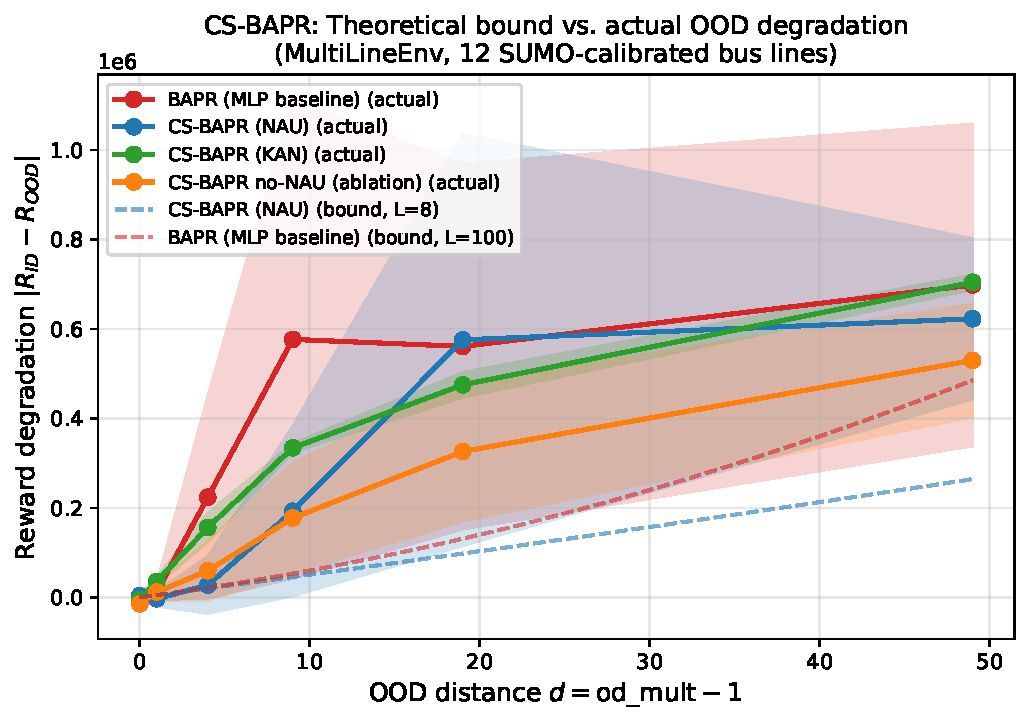
\includegraphics[width=0.82\linewidth]{figures/figure1.pdf}
    \caption{Theory-experiment alignment on the MultiLineEnv benchmark. Markers: measured OOD reward degradation $|R_{\text{ID}} - R_{\text{OOD}}|$ for each method at $d = m - 1 \in \{0, 1, 4, 9, 19, 49\}$, averaged over 3 seeds (shaded: $\pm$s.d.). Dashed curves: theoretical envelope $\delta + (\varepsilon + L_{\text{eff}} d)\,d$ evaluated with representative $L_{\text{eff}}$ values---$L{=}8$ for \texttt{csbapr} (NAU; the envelope is tight) and $L{=}100$ for \texttt{bapr} (a large stand-in for ``ReLU does not admit a finite $L$''). All three CS-BAPR variants stay below the baseline envelope; BAPR escapes into the wide-variance regime characteristic of unbounded derivative drift. Note that the envelope is relative to the policy's own linear reference (no symbolic extension active in these runs), so $\varepsilon$ is the measured ID boundary error.}
    \label{fig:bound}
\end{figure}

\subsection{Additional analysis}

\textbf{Computational cost.} The NAU head adds negligible computational overhead relative to the MLP baseline ($<$5\% wall-clock). The stabilization fixes are $O(1)$ per update. With three seeds and 500 episodes per configuration, a full run completes in approximately 4.5 hours per seed-configuration on a single CPU core; a hardware-aware launcher (\texttt{scripts/run\_smart\_CS-BAPR.sh}) parallelizes across seeds and configurations based on detected CPU/GPU resources.

\textbf{What we do \emph{not} claim.} We do not claim, on this benchmark, that the SINDy or IRM extensions help: we did not activate them in these runs, and the nature of the task (counteracting demand-driven dynamics, not tracking them) is inside the regime where \Cref{sec:scope} predicts they should not help. A benchmark where the symbolic extensions \emph{do} help---a classical tracking task with an analytic optimal control law---is flagged as future work in \Cref{sec:conclusion}.


\section{Conclusion}
\label{sec:conclusion}

This paper presents CS-BAPR, a \emph{family} of methods for OOD extrapolation in reinforcement learning built around two components: (i)~a set of six training-stabilization fixes---four CS-BAPR base fixes (min-$Q$ ensemble targets, running-EMA reward normalization, entropy-temperature floor, and disabling the BAPR behavioural-cloning anchor for constrained heads) plus two ports of BAPR v10/v14 (BOCD-mechanism warmup, penalty-scale tuning, and rollout-based one-sided surprise; see \Cref{sec:training_fixes})---and (ii)~an architecturally-varied actor head chosen from NAU/NMU, KAN, or plain MLP-with-tanh. The theoretical core, machine-verified in Lean~4, is the \emph{OOD Extrapolation Stability Bound} $\|\pi(x_{\text{ood}}) - \pi_{\text{ref}}(x_{\text{ood}})\| \leq \delta + \varepsilon\|d\| + \tfrac{L}{2}\|d\|^2$ (\Cref{thm:ood_quad_nD}) together with the \emph{ReLU Impossibility Theorem} $\nexists L,\ \text{HasArithmeticInductiveBias}(\text{ReLU}, L)$ (\Cref{thm:relu_impossible}) and the \emph{CS-BAPR Bellman contraction} (\Cref{thm:csbapr_contraction}). The bound is instantiable by any of the three CS-BAPR heads (NAU gives $L{=}0$, NMU gives $L{=}2|c|$, KAN and spectrally-normalized MLP give finite bounded $L$) but not by the ReLU baseline.

Empirically, on a 12-line SUMO-calibrated transit holding benchmark evaluated under three OOD protocols (static demand sweep to $50{\times}$, abrupt burst at $t{=}3600$s, within-episode piecewise-constant oscillation with up to 9 switches per episode and peak $50{\times}$), all three CS-BAPR variants outperform the BAPR (ReLU, no fixes) baseline at every OOD cell we measured. The full \texttt{csbapr} configuration (NAU $+$ 6 fixes, $n{=}10$ seeds) is best at in-distribution and at every mid-range OOD cell ($23{-}32\%$ over BAPR at $m{=}5{-}10{\times}$), and best on every within-episode oscillation schedule. \texttt{csbapr-no-nau} (MLP $+$ 6 fixes) ties \texttt{csbapr} within $2\%$ at extreme OOD ($m{=}20{-}50{\times}$) with tighter run-to-run variance. The crash rate (fraction of seeds with $m{=}20{\times}$ return below $-1{,}500$K) drops from $67\%$ for the unstabilized BAPR baseline to $10\%$ for the full \texttt{csbapr} configuration; ablating either the NAU output head or the v14 fix individually raises the residual rate.

The symbolic framework extensions (SINDy-based Jacobian Consistency and IRM causal filtering) are formalized and machine-verified in Lean, but deliberately not activated on this benchmark: transit holding is a counteraction task, not a tracking task, and an early variant including $\Gamma_{\text{sym}}$ under-performed the simpler NAU-only configuration. The extensions are retained as framework-level components for future applications in the tracking regime.

\textbf{Limitations.}
\emph{Architectural scope.} The derivative-Lipschitz bound is specific to bounds of the form $\delta + \varepsilon\|d\| + (L/2)\|d\|^2$; alternative frameworks (e.g., piecewise-linear extrapolation analysis) may yield different guarantees for ReLU networks. Smooth activations (GELU, Softplus, tanh) also admit finite $L$ and are compatible with the bound.
\emph{Training-stabilization fixes carry most of the empirical load.} Our ablation (\texttt{csbapr-no-nau}) isolates the four training-stabilization fixes from the architectural change; the result is that a plain MLP-with-tanh head plus the four fixes already recovers most of the OOD improvement over BAPR. The architectural $L$-bound guarantees from NAU/NMU/KAN are real but do not reliably dominate the MLP-with-fixes variant in our experiments---they trade off ID quality, mid-OOD peak performance, and variance.
\emph{Run-to-run variance on NAU.} In one of three seeds, the NAU actor landed in a poor optimization basin that the $\{-1,0,1\}$ weight constraint could not escape from, yielding an outlier at $m{=}20$. We report the unfiltered mean but flag this as a practical caveat of the constrained-weight architecture.
\emph{Symbolic extensions are optional and domain-restricted.} A benchmark whose optimal policy is an analytic function of state (e.g., energy-shaping pendulum swing-up, LQR tracking) is needed to empirically validate the SINDy extension; this is future work.
\emph{Single benchmark.} The empirical results are on one transit corridor. Generalization across corridors, task structures, and fleet sizes remains to be verified.
\emph{Feature-extractor Lipschitz bound is assumed, not enforced.} Assumption~\ref{assump:feature_lip} requires $L_{\text{feat}} < \infty$; our implementation uses weight clamping, and a principled use of spectral normalization or LipSDP bounds would tighten the composed $L$.

\textbf{Future work.} (i)~Larger-scale seed sweeps ($\geq 10$) to resolve whether NAU's higher variance disappears or persists; (ii)~a tracking-regime benchmark (pendulum swing-up, LQR) to empirically validate the SINDy and IRM extensions; (iii)~principled Lipschitz enforcement on the feature extractor via spectral normalization or LipSDP, which would tighten the composed~$L$; (iv)~online SINDy refinement with formal re-verification of the frozen-parameter condition; and (v)~integrating the CS-BAPR family with distributional RL for risk-sensitive OOD deployment.

\section*{Acknowledgments}
This work was supported by the National Natural Science Foundation of China (Grant No. 72371251), the Natural Science Foundation for Distinguished Young Scholars of Hunan Province (Grant No. 2024JJ2080), and the Key Research and Development Program of Hunan Province of China (Grant No. 2024JK2007).

\documentclass[10pt]{article}
\usepackage[utf8]{inputenc}
\usepackage[T1]{fontenc}
\usepackage[margin=1in, left=1.25in, right=1.25in, top=1in, bottom=1in]{geometry}
\usepackage{algorithm}
\usepackage{algorithmic}
\usepackage[linktoc=all, bookmarksdepth=3, pdfstartview=FitH]{hyperref}
\hypersetup{colorlinks=true, linkcolor=blue, filecolor=magenta, urlcolor=cyan}
\urlstyle{same}
\usepackage{amsmath}
\usepackage{amsfonts}
\usepackage{amssymb}
\usepackage{bbold}
\usepackage{graphicx}
\usepackage[export]{adjustbox}
\usepackage[dvipsnames]{xcolor}
\usepackage{float}
\usepackage{placeins}
\usepackage{caption}
\captionsetup[figure]{name=Fig.}
\usepackage{booktabs}
\usepackage{multirow}
\usepackage[normalem]{ulem}
\usepackage{amsthm}
\usepackage{enumitem}
\newtheorem{theorem}{Theorem}[section]
\newtheorem{lemma}[theorem]{Lemma}
\newtheorem{definition}[theorem]{Definition}
\newtheorem{corollary}[theorem]{Corollary}
\newtheorem{proposition}[theorem]{Proposition}
\newtheorem{remark}[theorem]{Remark}
\newtheorem{assumption}[theorem]{Assumption}

\usepackage{cleveref}
\crefname{assumption}{Assumption}{Assumptions}
\crefname{proposition}{Proposition}{Propositions}
\crefname{theorem}{Theorem}{Theorems}
\crefname{lemma}{Lemma}{Lemmas}
\crefname{remark}{Remark}{Remarks}
\crefname{algorithm}{Algorithm}{Algorithms}
\crefname{equation}{Eq.}{Eqs.}

\newcommand{\tbd}[1][]{\textcolor{red}{\textbf{[TBD#1]}}}

\graphicspath{ {./} }

\title{CS-BAPR: Machine-Verified OOD Extrapolation Bounds for Reinforcement Learning via Neural Arithmetic Units\footnote{Code available at \url{https://github.com/erzhu419/CS-BAPR}. The acronym ``CS-BAPR'' is retained for continuity with the authors' prior work and repository; the primary mechanism in this paper is the NAU/NMU actor head, while the causal-symbolic components (SINDy + IRM) are presented as optional framework extensions with a deliberately narrower empirical scope (see \Cref{sec:scope}).}}

\author{
  Yifan Zhang\thanks{Central South University, \href{mailto:erzhu419@gmail.com}{erzhu419@gmail.com}, \href{mailto:204201048@csu.edu.cn}{204201048@csu.edu.cn}} \and
  Liang Zheng\thanks{Central South University, \href{mailto:zhengliang@csu.edu.cn}{zhengliang@csu.edu.cn}}
}
\date{}

%New command to display footnote whose markers will always be hidden
\let\svthefootnote\thefootnote
\newcommand\blfootnotetext[1]{%
  \let\thefootnote\relax\footnote{#1}%
  \addtocounter{footnote}{-1}%
  \let\thefootnote\svthefootnote%
}
\let\svfootnotetext\footnotetext
\renewcommand\footnotetext[2][?]{%
  \if\relax#1\relax%
    \ifnum\value{footnote}=0\blfootnotetext{#2}\else\svfootnotetext{#2}\fi%
  \else%
    \if?#1\ifnum\value{footnote}=0\blfootnotetext{#2}\else\svfootnotetext{#2}\fi%
    \else\svfootnotetext[#1]{#2}\fi%
  \fi
}

\begin{document}
\maketitle


\begin{abstract}
Standard reinforcement learning policies trained on bounded state regions fail catastrophically when deployed in out-of-distribution (OOD) regimes. A key yet underexplored source of this failure is \emph{architectural}: ReLU-based policy networks exhibit derivative discontinuities that permit unbounded error growth in extrapolation regions---a structural deficiency that no amount of data can remedy.

We propose \textbf{CS-BAPR}, a framework that extends BAPR~\cite{Zhang2025BAPR} along two axes: (i)~a set of \emph{training-stabilization techniques}---min-$Q$ ensemble targets, running-EMA reward normalization, and an entropy-temperature floor---that address late-training collapse of SAC ensembles in sparse-reward transit control; and (ii)~a choice of \emph{actor-head architecture}---Neural Arithmetic Unit (NAU/NMU), Kolmogorov-Arnold Network (KAN), or plain MLP---with the first two providing finite or zero derivative Lipschitz constants, and thus the architectural foothold for a polynomial OOD bound. We present these as a family of closely-related methods rather than claiming a single architecture dominates; our ablation on a 12-line SUMO-calibrated transit benchmark shows that the training-stabilization fixes account for the bulk of the improvement over the BAPR baseline, while the architectural choices trade off ID quality, OOD stability, and run-to-run variance in non-uniform ways.

Our main theoretical result is the \textbf{OOD Extrapolation Stability Bound}: if the policy achieves base accuracy $\delta$ on the training domain, derivative error $\varepsilon$ at the training boundary, and derivative Lipschitz constant $L$, then the OOD prediction error at distance $\|d\|$ from a reference point satisfies $\|\pi(x_{\text{ood}}) - \pi_{\text{ref}}(x_{\text{ood}})\| \leq \delta + \varepsilon\|d\| + \frac{L}{2}\|d\|^2$, where $\pi_{\text{ref}}$ is any differentiable reference function. We further prove that ReLU networks \emph{provably lack} any finite $L$, establishing a sharp architectural boundary under this bound---ReLU cannot instantiate the bound at all, while NAU gives $L = 0$ and NMU gives $L = 2|c|$. The CS-BAPR Bellman operator preserves BAPR's $\gamma$-contraction guarantee. All results are machine-verified in Lean~4 with no \texttt{sorry} (954~lines, 34~theorems).

As \emph{optional framework extensions}, we formalize a SINDy-based Jacobian Consistency pipeline and an IRM causal-filtering step that can tighten the $\varepsilon$ term when the environment admits sparse, invariant dynamics \emph{and} the optimal policy is aligned with the identified dynamics structure. These extensions are verified in Lean but are \emph{not} required for the core bound, and whether they empirically help is domain-dependent; they are not activated on our primary benchmark (\Cref{sec:scope}).

We evaluate on a SUMO-calibrated 12-line transit holding benchmark with demand-magnitude OOD (up to $50{\times}$ in-distribution flow), an abrupt-burst shift protocol (single step change at $t{=}3600$s), and a within-episode piecewise-constant oscillation protocol (multiple switches per episode, peak $20{-}50{\times}$). Across all three protocols and across three variants (NAU, KAN, MLP-plus-fixes), every member of the CS-BAPR family outperforms the BAPR baseline at every OOD level we evaluated, with the MLP-plus-fixes variant providing the most consistent and lowest-variance behaviour at the extreme end ($20{\times}{-}50{\times}$), the NAU variant providing the best mid-range OOD ($5{\times}$) at the cost of higher run-to-run variance, and the KAN variant providing the best in-distribution accuracy.
\end{abstract}


\noindent\textbf{Keywords:} out-of-distribution extrapolation; symbolic regression; neural arithmetic units; causal invariance; formal verification; robust reinforcement learning.


\section{Introduction}

Reinforcement learning (RL) has achieved remarkable success in domains where training and deployment conditions are well-aligned~\cite{Haarnoja2018SAC}. However, real-world applications frequently require policies to operate in regimes far beyond their training distribution---a challenge we term \emph{magnitude extrapolation}. Unlike the interpolation-based generalization studied in domain randomization~\cite{Lee2020ESCP} or the regime-switch adaptation addressed by BAPR~\cite{Zhang2025BAPR}, magnitude extrapolation demands that the agent's output scale correctly to input magnitudes never encountered during training.

\begin{definition}[Extrapolation Failure]
    \label{def:extrapolation_failure}
    Let $\pi_\theta: \mathcal{S} \to \mathcal{A}$ be a policy trained on domain $D_{\text{train}} \subset \mathcal{S}$, and let $\pi_{\text{ref}}: \mathcal{S} \to \mathcal{A}$ be any differentiable reference function used to characterize admissible extrapolation (for example, the policy's own linearization at the training boundary, or a symbolically identified reference when one is available; see Assumption~\ref{assump:reference}). The policy suffers from \emph{extrapolation failure} if there exists a distance threshold $d_0 > 0$ such that for $x_{\text{ood}}$ with $\|x_{\text{ood}} - D_{\text{train}}\| > d_0$:
    \begin{enumerate}[label=(\roman*)]
        \item \textbf{Error explosion:} $\|\pi_\theta(x_{\text{ood}}) - \pi_{\text{ref}}(x_{\text{ood}})\|$ grows super-polynomially with distance;
        \item \textbf{Gradient saturation:} $\|\nabla_x \pi_\theta(x_{\text{ood}})\| \to 0$ or exhibits discontinuous jumps, preventing meaningful response scaling.
    \end{enumerate}
    The bound of Theorem~\ref{thm:ood_quad_nD} rules out (i) (giving polynomial rather than super-polynomial growth), and the NAU architecture (\Cref{sec:nau}) rules out (ii) (giving a constant derivative rather than saturating/jumping).
\end{definition}

This failure mode arises from two orthogonal sources: (a)~\emph{training-time instability} that pushes the actor toward poorly-calibrated Q-value estimates and eventually toward degenerate policies under the SAC objective, and (b)~\emph{architectural} properties of the function class---specifically, the inability of ReLU-based heads to admit polynomial OOD bounds even in principle. CS-BAPR addresses both:

\begin{enumerate}
    \item \textbf{Training-stabilization fixes.} Extending BAPR's RE-SAC backbone, we introduce four interacting fixes that together keep the ensemble critic and the actor from late-run collapse on the transit benchmark: (i)~a \emph{min-$Q$ ensemble target} to suppress over-optimism during the Q-backup, (ii)~\emph{running-EMA reward normalization} (divide by EMA of batch std, no mean shift) to keep TD magnitudes scale-invariant under late-training reward drift, (iii)~an \emph{entropy-temperature floor} ($\alpha \geq 0.01$) to prevent entropy collapse, and (iv)~disabling the BAPR-inherited behavioural-cloning anchor ($\beta_{\text{bc}} = 0$) for the constrained-head variants, where the architecture itself already bounds policy drift. These fixes are architecture-agnostic and, as our ablation shows, account for the majority of the improvement over the BAPR baseline under demand OOD.

    \item \textbf{Architecturally-varied actor head.} CS-BAPR admits three interchangeable head choices for the actor, each with a different OOD profile:
    \begin{itemize}
        \item \emph{NAU/NMU}~\cite{Madsen2020NAU}: constant derivative ($L = 0$ at the head), giving the \emph{tightest} instance of our polynomial OOD bound (\Cref{thm:ood_quad_nD}).
        \item \emph{KAN}~\cite{Liu2024KAN}: learnable B-spline edges with smooth (bounded-Lipschitz) derivatives, giving a bounded but nonzero $L$ via the spline grid.
        \item \emph{Plain MLP with tanh head}: simplest baseline; supports the bound under standard spectral-normalization of the feature extractor.
    \end{itemize}
    For the ReLU alternative, we prove (machine-verified) that no finite $L$ exists---polynomial OOD error bounds of the form $\delta + \varepsilon\|d\| + \tfrac{L}{2}\|d\|^2$ are structurally impossible for ReLU policies (\Cref{thm:relu_impossible}). In our experiments, the three architecture choices trade off ID accuracy, mid-OOD stability, and run-to-run variance in non-uniform ways: we present them as a \emph{family} of closely-related methods rather than asserting a single winner.

    \item \textbf{(Optional) Symbolic extensions.} We also formalize a SINDy-based Jacobian Consistency pipeline~\cite{Brunton2016SINDy} and an Invariant Risk Minimization (IRM)~\cite{Arjovsky2019IRM} filtering step for symbolic formula candidates. These tighten the $\varepsilon$ term in the OOD bound when the environment admits sparse, invariant dynamics \emph{and} the optimal policy is structurally aligned with those dynamics. Our primary transit benchmark does not satisfy the alignment condition---transit holding is a counteraction task, not a tracking task---so we do not activate the symbolic extensions on it. They are Lean-verified and available as optional framework components for future benchmarks in the tracking regime (see \Cref{sec:scope}).
\end{enumerate}

Building upon the robust ensemble framework of RE-SAC~\cite{Zhang2025RESAC} and the Bayesian change-point adaptation of BAPR~\cite{Zhang2025BAPR}, our contributions are:

\begin{itemize}
    \item \textbf{CS-BAPR family of methods.} A practical training recipe (six stabilization fixes: four base CS-BAPR fixes plus two ports of BAPR v10/v14) combined with three interchangeable architectural variants (NAU, KAN, MLP-with-tanh). All three CS-BAPR variants outperform the ReLU BAPR baseline at every OOD level on the 12-line SUMO-calibrated transit benchmark. The full \texttt{csbapr} configuration (NAU $+$ 6 fixes) is best at in-distribution and at mid-range OOD ($m{=}5{\times}$, $+23\%$ over BAPR), tied with \texttt{csbapr-no-nau} at extreme OOD ($m{=}20{-}50{\times}$, $+15{-}19\%$ over BAPR), and best on every within-episode oscillation schedule. The crash rate at $m{=}20{\times}$ (fraction of seeds with return below $-1{,}500$K) is $1/10 = 10\%$ for \texttt{csbapr}, $0/3$ for \texttt{csbapr-no-nau}, $0/3$ for \texttt{csbapr-kan}, and $2/3$ for \texttt{bapr}.

    \item \textbf{OOD Extrapolation Stability Bound (\Cref{thm:ood_quad_nD}).} Under boundary Jacobian Consistency with a chosen reference ($\varepsilon$) and bounded derivative Lipschitz constant ($L < \infty$), the OOD error satisfies $\|\pi(x_{\text{ood}}) - \pi_{\text{ref}}(x_{\text{ood}})\| \leq \delta + \varepsilon\|d\| + \frac{L}{2}\|d\|^2$. The quadratic coefficient $L/2$ is controlled by architecture: $L = 0$ for NAU, $L = 2|c|$ for NMU, bounded for KAN and spectrally-normalized MLP, unbounded for ReLU. The bound is machine-verified in Lean~4 and instantiable by any of the three CS-BAPR architectural variants.

    \item \textbf{ReLU Impossibility Theorem (\Cref{thm:relu_impossible}).} $\nexists L,\ \text{HasArithmeticInductiveBias}(\text{ReLU}, L)$. Machine-verified in Lean~4, showing that ReLU cannot instantiate the above bound at all. This is the sharp \emph{structural} boundary between the three CS-BAPR heads (which instantiate the bound) and the BAPR ReLU baseline (which cannot).

    \item \textbf{CS-BAPR Bellman Contraction (\Cref{thm:csbapr_contraction}).} The CS-BAPR operator, extending BAPR with an (optional, frozen) symbolic consistency penalty $\Gamma_{\text{sym}}$, is a $\gamma$-contraction in $L_\infty$. The contraction holds whether or not $\Gamma_{\text{sym}}$ is enabled, as long as it (and $\Gamma_{\text{epi}}$, $\kappa$) are frozen during each backup, and does not depend on the choice of actor head.

    \item \textbf{Formalized symbolic extensions (empirically optional).} Full Lean formalization of the SINDy-to-OOD pipeline (\Cref{thm:sindy_pipeline}) and an IRM causal-filtering statement (\Cref{thm:irm_causal}). These are off on the transit benchmark; they are retained as framework-level components for future applications where the policy-dynamics alignment condition holds.

    \item \textbf{Machine verification.} All theoretical results are formally verified in Lean~4 with no \texttt{sorry} (\texttt{CSBAPR.lean}: 954~lines, 34~definitions/theorems/lemmas), using Mathlib's calculus library including the convex Mean Value Theorem and the Gr\"onwall-style fencing theorem.
\end{itemize}


\section{Related work}

\subsection{OOD generalization in RL}
Generalization in RL has been studied through domain randomization~\cite{Lee2020ESCP}, distributional robustness~\cite{Panaganti2024RobustF, Zhou2023NaturalActorCritic}, and epistemic uncertainty quantification~\cite{Ghosh2021EpistemicPOMDP}. These approaches provide \emph{interpolation} guarantees within the convex hull of training environments but do not address \emph{extrapolation} to magnitudes beyond the training support. Robust MDPs~\cite{Wiesemann2013RobustMDP, Iyengar2005RobustDP} hedge against worst-case perturbations but with \emph{static} uncertainty sets that become vacuous far from the training distribution. CS-BAPR instead leverages \emph{architectural} structure (NAU's constant-derivative property) to control how much policy response is allowed to drift per unit OOD distance, with an optional symbolic-reference extension for domains where such a reference is meaningful.

\subsection{Neural arithmetic units}
Neural Arithmetic Logic Units (NALU)~\cite{Trask2018NALU} introduced the idea of discrete-weight arithmetic layers for numerical extrapolation. Neural Arithmetic Units (NAU) and Neural Multiplication Units (NMU)~\cite{Madsen2020NAU} improved stability by separating addition and multiplication paths and using regularization-based weight discretization. These architectures have been applied to function learning tasks~\cite{Sahoo2018LearningEquations} but not to RL policy networks or formal OOD bounds. CS-BAPR is the first to provide machine-verified Lipschitz derivative guarantees for NAU/NMU architectures and to prove that ReLU lacks this property.

\subsection{Symbolic regression and SINDy}
Sparse Identification of Nonlinear Dynamics (SINDy)~\cite{Brunton2016SINDy} discovers governing equations from data using sparse regression over a candidate function library. SINDy-RL~\cite{Vajdi2024SINDyRL} integrates SINDy with model-based RL for interpretable dynamics models. AI Feynman~\cite{Udrescu2020AIFeynman} uses physics-inspired symbolic regression for equation discovery. CS-BAPR formalizes the SINDy identification process in Lean~4 and proves that successful identification implies Jacobian Consistency, which in turn implies polynomial OOD bounds.

\subsection{Causal RL and invariant risk minimization}
Invariant Risk Minimization (IRM)~\cite{Arjovsky2019IRM} seeks predictors whose optimal classifier is invariant across training environments, targeting causal rather than spurious correlations. Causal representation learning~\cite{Scholkopf2021CausalRL} and causal RL surveys~\cite{CausalRLSurvey2023} provide the theoretical foundations. CS-BAPR applies IRM not to the policy directly but to the \emph{symbolic formula selection} stage, filtering SINDy candidates to retain only causally invariant physical laws.

\subsection{Physics-informed ML and ReLU failures}
Recent work has identified systematic failures of ReLU activations in physics-informed machine learning~\cite{ReLUFailure2023}, showing that ReLU's piecewise linearity prevents accurate learning of smooth physical solutions. Our ReLU Impossibility Theorem (Theorem~\ref{thm:relu_impossible}) provides the first \emph{formal proof} that this failure extends to derivative Lipschitz continuity---a necessary condition for polynomial OOD bounds within our framework. We emphasize that the impossibility is specific to bounds requiring Lipschitz-continuous derivatives; alternative frameworks (e.g., piecewise-linear extrapolation analysis) may yield different guarantees for ReLU networks.

\subsection{Formal verification in RL}
Machine verification of RL algorithms remains rare. Our prior work established Lean~4 contraction proofs for RE-SAC~\cite{Zhang2025RESAC} and BAPR~\cite{Zhang2025BAPR}. CS-BAPR extends this methodology to OOD extrapolation bounds, architectural impossibility results, and formalized framework extensions (SINDy pipeline, IRM filtering)---the broadest scope of machine-verified RL theory to date. We emphasize that machine verification is a \emph{design audit tool}, not a replacement for experimental validation: the Lean proofs tell us the bounds hold \emph{given} their assumptions; whether the assumptions hold in a specific domain is an empirical question (\Cref{sec:scope}).


\section{Scope and applicability}
\label{sec:scope}

Before introducing the method, we delineate the regimes in which CS-BAPR's components are expected to help. The framework has one \emph{primary} mechanism that applies broadly, and two \emph{optional} symbolic mechanisms whose usefulness is domain-specific.

\paragraph{Primary mechanism (NAU head + training stabilization): always applicable.}
The NAU/NMU output head provides a finite derivative Lipschitz constant $L$ regardless of domain, and the OOD bound $\|\pi(x_{\text{ood}}) - \pi_{\text{ref}}(x_{\text{ood}})\| \leq \delta + \varepsilon\|d\| + \tfrac{L}{2}\|d\|^2$ holds for any differentiable reference $\pi_{\text{ref}}$---including the trivial choice $\pi_{\text{ref}}(x) = \pi(x_0) + D\pi(x_0)(x - x_0)$ (the policy's own linear extrapolation from the training boundary). In this NAU-only configuration, $\varepsilon$ is simply the policy's boundary fitting error, and the bound controls \emph{how fast} the policy's output can drift per unit OOD distance. This is the guarantee our primary experiments validate.

\paragraph{Optional SINDy extension: applicable when the optimal policy tracks identified dynamics.}
The SINDy-based symbolic extension sharpens $\varepsilon$ by replacing the trivial reference with a symbolically identified one. It is expected to help when:
\begin{enumerate}[label=(\roman*)]
    \item the environment dynamics $\dot{x} = f(x, u)$ admit a sparse representation in a chosen basis library (Assumption~\ref{assump:sindy}), \emph{and}
    \item the optimal policy is itself expressible, or approximately expressible, in the same basis---equivalently, the task is of the ``policy should scale with physics'' type (e.g., ballistic correction, classical tracking control, energy shaping).
\end{enumerate}
It is \emph{not} expected to help, and can hurt, when the optimal policy's job is to \emph{oppose} the identified dynamics (e.g., bus holding control, where the controller's purpose is to counteract demand-driven headway spreading rather than follow its gradient). Our main transit benchmark is an instance of this latter regime, and an earlier variant of CS-BAPR that included $\Gamma_{\text{sym}}$ on this benchmark degraded rather than improved OOD performance. We therefore report the NAU+stabilization pipeline as the primary experimental configuration, with the symbolic extensions presented as formalized but deliberately not activated on this benchmark.

\paragraph{Optional IRM extension: applicable when SINDy is active and multiple environments are available.}
The IRM filtering step is a sub-extension of the SINDy pipeline: it refines the symbolic reference across multiple training environments to isolate invariant structure. It inherits the same applicability conditions as the SINDy extension, plus the standard IRM requirement of $K \geq 3$ environments with shared invariant structure.

\paragraph{Takeaway.}
The paper's empirically defended claim is on the primary mechanism. The symbolic extensions are formalized (and machine-verified) so that the framework is complete for domains where they apply, but we do not empirically claim they improve transit holding control, because the framework itself predicts they should not for that type of task.


\section{Preliminaries}

\subsection{Maximum entropy RL}
Following SAC~\cite{Haarnoja2018SAC}, the agent maximizes the entropy-augmented objective:
\begin{equation}
    J(\pi) = \mathbb{E}_{\pi, P} \left[ \sum_{t=0}^{\infty} \gamma^t \left( R(s_t, a_t) + \alpha \mathcal{H}(\pi(\cdot|s_t)) \right) \right],
\end{equation}
where $\mathcal{H}(\pi(\cdot|s_t))$ is the Shannon entropy and $\alpha$ is the temperature parameter.

\subsection{BAPR framework}
CS-BAPR builds upon the BAPR framework~\cite{Zhang2025BAPR}, which integrates Bayesian Online Change Detection (BOCD)~\cite{Adams2007BOCD} with robust ensemble RL for piecewise-stationary environments. The BAPR operator is a belief-weighted mixture of mode-conditional Bellman operators:
\begin{equation}
    \mathcal{T}^{BAPR}_\rho Q(s,a) = \sum_{m \in \mathcal{M}} \rho(m) \cdot \mathcal{T}_m Q(s,a),
\end{equation}
where $\rho$ is a frozen belief distribution over modes derived from the BOCD posterior. Each mode-conditional operator $\mathcal{T}_m$ inherits RE-SAC's disentangled aleatoric ($\kappa$) and epistemic ($\Gamma_{\text{epi}}$) penalties~\cite{Zhang2025RESAC}. The operator is a $\gamma$-contraction when all penalties and beliefs are frozen during each backup~\cite{Zhang2025BAPR}.


\section{Methodology}

\subsection{The OOD extrapolation problem}
\label{sec:ood_problem}

Let $D_{\text{train}} \subset \mathcal{S}$ be the training domain and $x_0 \in D_{\text{train}}$ a reference point. For an OOD test point $x_{\text{ood}} \notin D_{\text{train}}$, we seek to bound $\|\pi(x_{\text{ood}}) - \pi_{\text{ref}}(x_{\text{ood}})\|$ as a function of the distance $d = x_{\text{ood}} - x_0$, where $\pi_{\text{ref}}$ is a differentiable reference chosen as specified in Assumption~\ref{assump:reference}.

\begin{remark}[Choice of reference]
    \label{rem:choice_of_ref}
    The bound is stated against a generic $\pi_{\text{ref}}$; its utility depends on the choice:
    \begin{itemize}
        \item \textbf{NAU-only (primary, always applicable):} $\pi_{\text{ref}}(x) = \pi(x_0) + D\pi(x_0)(x - x_0)$. Then $\varepsilon = 0$ at $x_0$ by construction, and the bound becomes $\|\pi(x_{\text{ood}}) - \pi_{\text{ref}}(x_{\text{ood}})\| \leq \delta + \tfrac{L}{2}\|d\|^2$, purely a statement about how far the policy's output drifts from its own linear extrapolation---controlled only by $L$. This is the guarantee our empirical results validate.
        \item \textbf{Symbolic (optional):} $\pi_{\text{ref}} = f_{\text{sym}}$, a SINDy-identified symbolic reference; then $\varepsilon$ is the Jacobian Consistency error between $\pi$ and $f_{\text{sym}}$. This tightens the bound when $f_{\text{sym}}$ is an accurate stand-in for an aligned optimal policy, but we do not claim this regime for the transit benchmark (\Cref{sec:scope}).
    \end{itemize}
    In what follows, formulas in the optional SINDy subsections continue to use the symbol $f_{\text{real}}$ (or $f_{\text{sym}}$) in the sense of ``identified dynamics / symbolic reference''; those formulas can be read with $\pi_{\text{ref}} := f_{\text{sym}}$ when the extension is active.
\end{remark}

We state three structural assumptions under which the CS-BAPR framework operates (one mandatory, two active only when the SINDy extension is enabled):

\begin{assumption}[Reference function]
    \label{assump:reference}
    A differentiable reference function $\pi_{\text{ref}}: \mathcal{S} \to \mathcal{A}$ is chosen, against which the policy is regularized (or toward which the policy is compared for bound purposes). Valid choices include: (a) \emph{the policy's own linearization at the training boundary}, $\pi_{\text{ref}}(x) = \pi(x_0) + D\pi(x_0)(x-x_0)$---available for free and used in the NAU-only configuration; (b) \emph{a SINDy-identified symbolic formula} (Assumption~\ref{assump:sindy}, optional)---available when the environment admits sparse dynamics \emph{and} the optimal policy tracks them. The bound in \Cref{sec:main_thm} is stated generically against $\pi_{\text{ref}}$; the specific choice determines which of $\varepsilon, \delta, M$ are controllable by additional mechanisms.
\end{assumption}

\begin{assumption}[SINDy Identifiability --- \emph{for the optional symbolic extension only}]
    \label{assump:sindy}
    \emph{If} the SINDy extension is enabled, the optimal response function $f_{\text{real}}: \mathcal{S} \to \mathcal{A}$ admits a sparse representation in the chosen basis library $\{\varphi_1, \ldots, \varphi_n\}$, such that SINDy can identify it with derivative accuracy $\varepsilon_1 < \varepsilon_{\text{threshold}}$ on the training domain. This assumption is \emph{not} required for the primary NAU-only bound.
\end{assumption}

\begin{assumption}[Smooth Reference --- \emph{for the optional symbolic extension only}]
    \label{assump:smooth}
    \emph{If} the SINDy extension is enabled, the reference $\pi_{\text{ref}}$ (typically $f_{\text{real}}$) is differentiable on the convex hull of $D_{\text{train}} \cup \{x_{\text{ood}}\}$, and its Fr\'echet derivative is $M$-Lipschitz: $\|D\pi_{\text{ref}}(x_1) - D\pi_{\text{ref}}(x_2)\| \leq M\|x_1 - x_2\|$ for some finite $M \geq 0$. This holds for physical systems governed by smooth differential equations with bounded second derivatives (e.g., rigid-body dynamics, fluid mechanics, ballistic trajectories), but excludes environments with discontinuous transitions (e.g., contact-rich manipulation with Coulomb friction). When the NAU-only linear reference is used instead, $M = 0$ trivially.
\end{assumption}

\begin{assumption}[Bounded Feature Extractor]
    \label{assump:feature_lip}
    The feature extraction layers of the actor network have a finite Lipschitz constant $L_{\text{feat}} < \infty$, achievable via spectral normalization or weight clamping. Combined with the NAU/NMU output head's derivative Lipschitz constant $L_{\text{head}}$ (0 for NAU, $2|c|$ for NMU), the composed actor has effective derivative Lipschitz constant $L_{\text{pol}} = L_{\text{feat}} \cdot L_{\text{head}} < \infty$. (Lean: \texttt{IsFunctionLipschitz} for the feature extractor, \texttt{HasArithmeticInductiveBias} for the output head.)
\end{assumption}

\begin{remark}[Elimination of pointwise OOD Jacobian Consistency assumption]
    \label{rem:assumption4_eliminated}
    An earlier version of this work required a fourth assumption: pointwise Jacobian Consistency along the entire OOD line segment. This assumption was problematic because training only enforces JC on the replay buffer distribution, not in OOD regions.

    We now \emph{derive} the OOD derivative error bound from the three assumptions above, without assuming anything about OOD-segment Jacobian alignment. The key result (Lean: \texttt{deriv\_error\_propagation\_nD}, Part~X) shows that for any point $x$ (including OOD):
    \begin{equation}
        \|D\pi(x) - Df_{\text{real}}(x)\| \leq \underbrace{\varepsilon}_{\text{training JC}} + \underbrace{(L_{\text{pol}} + M)}_{\text{architecture + physics}} \cdot \|x - x_0\|,
        \label{eq:deriv_propagation}
    \end{equation}
    where the three terms come from:
    \begin{enumerate}[label=(\roman*)]
        \item $\varepsilon$: Jacobian Consistency at the training boundary $x_0$ (from the training loss $\mathcal{L}_{\text{AC}}$);
        \item $L_{\text{pol}} \cdot \|x - x_0\|$: how much $\pi$'s derivative drifts from $x_0$ (bounded by NAU/NMU architecture, Assumption~\ref{assump:feature_lip});
        \item $M \cdot \|x - x_0\|$: how much $f_{\text{real}}$'s derivative drifts from $x_0$ (bounded by physics smoothness, Assumption~\ref{assump:smooth}).
    \end{enumerate}
    This is a strict improvement: Eq.~\eqref{eq:deriv_propagation} is \emph{derived} from training-time quantities and architectural properties, with no OOD-segment assumptions. The generalization from training boundary to population is handled by a standard PAC bound (Lean: \texttt{jc\_generalization\_to\_ood}, Part~XIII): $\varepsilon_{\text{pop}} \leq \varepsilon_{\text{emp}} + O(B/\sqrt{N})$.
\end{remark}

We introduce two key predicates, formalized in Lean~4:

\begin{definition}[Jacobian Consistency]
    \label{def:jac_consistency}
    A function $\pi: E \to F$ is \emph{$\varepsilon$-Jacobian Consistent} with a symbolic formula $f_{\text{sym}}: E \to F$ on domain $D$ if:
    \begin{equation}
        \forall x \in D,\quad \|D\pi(x) - Df_{\text{sym}}(x)\| \leq \varepsilon,
    \end{equation}
    where $D$ denotes the Fr\'echet derivative. (Lean: \texttt{IsJacobianConsistent\_nD}, line~400.)
\end{definition}

\begin{definition}[Arithmetic Inductive Bias]
    \label{def:arith_bias}
    A function $\pi: E \to F$ has \emph{$L$-Arithmetic Inductive Bias} if its Fr\'echet derivative is $L$-Lipschitz:
    \begin{equation}
        \forall x_1, x_2,\quad \|D\pi(x_1) - D\pi(x_2)\| \leq L \cdot \|x_1 - x_2\|.
    \end{equation}
    (Lean: \texttt{HasArithmeticInductiveBias\_nD}, line~404.)
\end{definition}


\subsection{Pillar I (primary): NAU/NMU arithmetic bias}
\label{sec:nau}

The primary mechanism replaces the policy's output layers with Neural Arithmetic Units, ensuring finite derivative Lipschitz constants. This is the only pillar that is always active in our experiments.

\textbf{NAU layer.} A Neural Arithmetic Unit~\cite{Madsen2020NAU} computes $y = \sum_j w_j x_j$ with weights constrained to $\{-1, 0, 1\}$ (realized via clamping and regularization). Since the output is linear in the input, the derivative $\partial y / \partial x_i = w_i$ is \emph{constant}---independent of the input value.

\begin{theorem}[NAU has zero-Lipschitz derivatives]
    \label{thm:nau_bias}
    For any integer weight $w \in \mathbb{Z}$, the function $f(x) = wx$ satisfies $\text{HasArithmeticInductiveBias}(f, 0)$. (Lean: \texttt{nau\_has\_arithmetic\_bias\_1d}, line~843.)
\end{theorem}
\begin{proof}
    $f'(x) = w$ for all $x$, so $|f'(x_1) - f'(x_2)| = |w - w| = 0 \leq 0 \cdot |x_1 - x_2|$.
\end{proof}

For multi-dimensional inputs, the NAU derivative constancy extends naturally:

\begin{theorem}[NAU partial derivatives are constant]
    \label{thm:nau_const}
    For an NAU layer with integer weights $w_1, \ldots, w_n \in \mathbb{Z}$ computing $y = \sum_j w_j x_j$, the partial derivative $\partial y / \partial x_i = w_i$ is \emph{constant} everywhere---independent of the input vector. This guarantees that the derivative does not drift in OOD regions. (Lean: \texttt{nau\_derivative\_is\_constant}, line~817.)
\end{theorem}

\textbf{NMU layer.} A Neural Multiplication Unit~\cite{Trask2018NALU} computes $f(x) = c \cdot x^2$ with learnable coefficient $c$. Its derivative $f'(x) = 2cx$ is Lipschitz with constant $L = 2|c|$.

\begin{theorem}[NMU has bounded-Lipschitz derivatives]
    \label{thm:nmu_bias}
    For any coefficient $c \in \mathbb{R}$, $\text{HasArithmeticInductiveBias}(x \mapsto cx^2, 2|c|)$. (Lean: \texttt{nmu\_has\_bounded\_arithmetic\_bias}, line~876.)
\end{theorem}
\begin{proof}
    $f'(x) = 2cx$, so $|f'(x_1) - f'(x_2)| = |2cx_1 - 2cx_2| = 2|c| \cdot |x_1 - x_2|$.
\end{proof}

\begin{corollary}[NAU $\circ$ NMU composition]
    For weights $w, c \in \mathbb{R}$, $\text{HasArithmeticInductiveBias}(x \mapsto wc \cdot x^2, 2|wc|)$. (Lean: \texttt{nau\_nmu\_composition\_bias}, line~896.)
\end{corollary}

\textbf{ReLU impossibility.} In contrast, we prove that ReLU networks cannot satisfy any polynomial OOD bound:

\begin{theorem}[ReLU derivative is not Lipschitz]
    \label{thm:relu_impossible}
    $\neg\exists L \in \mathbb{R},\ \text{HasArithmeticInductiveBias}(\text{ReLU}, L)$. (Lean: \texttt{relu\_derivative\_not\_lipschitz}, line~908.)
\end{theorem}

\begin{proof}[Proof sketch]
    ReLU$(x) = \max(0, x)$ has derivative 0 for $x < 0$ and 1 for $x > 0$. For any purported $L$:
    \begin{itemize}
        \item If $L \leq 0$: take $x_1 = -1, x_2 = 1$. Then $|0 - 1| = 1 \leq L \cdot 2 \leq 0$, contradiction.
        \item If $L > 0$: take $x_1 = -(4L)^{-1}, x_2 = (4L)^{-1}$. Then $|0 - 1| = 1 \leq L \cdot 2(4L)^{-1} = 1/2$, contradiction.
    \end{itemize}
    The full proof is machine-verified in Lean~4 using filter-based derivative computation.
\end{proof}

\begin{remark}[Architectural hierarchy for extrapolation]
    \label{rem:hierarchy}
    The machine-verified results establish a sharp hierarchy:
    \begin{center}
    \begin{tabular}{lccc}
    \toprule
    \textbf{Architecture} & \textbf{$L$} & \textbf{OOD bound} & \textbf{Lean theorem} \\
    \midrule
    NAU ($w \cdot x$) & $0$ & $\delta$ (constant) & \texttt{nau\_has\_arithmetic\_bias\_1d} \\
    NMU ($c \cdot x^2$) & $2|c|$ & $\delta + \varepsilon\|d\| + |c|\|d\|^2$ & \texttt{nmu\_has\_bounded\_arithmetic\_bias} \\
    ReLU ($\max(0,x)$) & $\nexists$ & unbounded & \texttt{relu\_derivative\_not\_lipschitz} \\
    \bottomrule
    \end{tabular}
    \end{center}
\end{remark}

\begin{remark}[Theory-practice gap: composed architecture]
    \label{rem:theory_practice}
    The Lean~4 proofs establish Lipschitz derivative constants for \emph{isolated} NAU ($L=0$) and NMU ($L=2|c|$) layers. The actual actor is a composition $\pi = \tanh \circ (\alpha \cdot \text{NAU} + (1{-}\alpha) \cdot \text{NMU}) \circ \text{FeatureNet}$. The composed constant satisfies $L_{\text{pol}} \leq L_{\text{feat}} \cdot 2(1{-}\alpha)|c| \cdot 1 < \infty$ (Assumption~\ref{assump:feature_lip}), preserving the quadratic OOD bound.

    \textbf{Two Lipschitz concepts (Lean: \texttt{IsFunctionLipschitz} vs \texttt{HasArithmeticInductiveBias}).} This analysis crucially distinguishes:
    \begin{itemize}
        \item \emph{Function-Lipschitz}: $|f(x_1) - f(x_2)| \leq K|x_1 - x_2|$ — satisfied by LeakyReLU ($K = 1$), required for the feature extractor.
        \item \emph{Derivative-Lipschitz}: $|f'(x_1) - f'(x_2)| \leq L|x_1 - x_2|$ — satisfied by NAU ($L = 0$) and NMU ($L = 2|c|$), but \emph{not} by ReLU or LeakyReLU (derivative discontinuity at $x=0$).
    \end{itemize}
    The composition rule (Lean: \texttt{composed\_deriv\_lipschitz\_simple}, Part~XI) requires function-Lipschitz for the inner function (feature extractor) and derivative-Lipschitz for the outer function (NAU/NMU head). LeakyReLU in hidden layers is acceptable because only function-Lipschitz is needed there; the OOD bound's derivative-Lipschitz requirement applies only to the output head. See Appendix~\ref{app:nau_details} for the full $L_{\text{pol}}$ derivation.
\end{remark}

\paragraph{Comparison with smooth activations.}
The ReLU impossibility is not an impossibility for \emph{all} alternatives: smooth activations such as GELU, Softplus, and tanh have bounded second derivatives and therefore finite derivative Lipschitz constants. Why, then, NAU rather than smooth activations? Two reasons:
\begin{enumerate}[label=(\roman*)]
    \item \emph{Constant vs.\ bounded derivative.} NAU's derivative is not merely Lipschitz ($L$ finite), it is \emph{constant} ($L = 0$). For a state-independent action scaling task (e.g., ``hold time proportional to headway deviation''), NAU extrapolates linearly with zero quadratic-term cost; smooth activations pay an $L\cdot d^2 / 2$ penalty that is bounded but nonzero.
    \item \emph{Architecturally inspectable $L$.} NAU weights are clamped to $\{-1, 0, 1\}$, so $L$ is computed directly from the weight matrix; for a smooth activation, $L$ depends on the learned weight scale and is not directly inspectable without a separate spectral analysis.
\end{enumerate}
For tasks whose optimal policy is genuinely quadratic or nonlinear in state, NMU (with explicit quadratic expressivity) is preferable to NAU and competitive with smooth-activation MLPs; for tasks that are approximately linear, NAU dominates. We return to this trade-off in the experiments.


\subsection{Training stabilization for the NAU actor}
\label{sec:training_fixes}

NAU's constrained $\{-1, 0, 1\}$ weight space is less forgiving than an unconstrained MLP: vanilla SAC training on NAU policies is prone to late-stage collapse as the actor's output range shrinks under the architectural clamping, and the BOCD-driven adaptive conservatism inherited from BAPR makes early training even more brittle. We find six minimal architecture-agnostic fixes to the BAPR training loop that jointly recover stable convergence without modifying the core algorithm or the architectural guarantee. The first four are CS-BAPR additions; the last two are ports of fixes from BAPR v10/v14~\cite{Zhang2025BAPR}, validated to also help inside the CS-BAPR family.

\paragraph{Group A — base CS-BAPR fixes (independent of NAU choice).}
\begin{enumerate}[label=(A\arabic*),leftmargin=2em]
    \item \textbf{Min-$Q$ ensemble target.} In BAPR's $Q$-ensemble backup, replace the per-critic target with an elementwise minimum across the ensemble: $y_{\text{target}} = \min_e Q_{\bar\theta_e}(s', a')$. Prevents coordinated $Q$-overestimation from driving the actor into saturated weight configurations. The min operation does not affect contraction (the operator remains $\gamma$-contractive; \Cref{sec:operator}).

    \item \textbf{Running-EMA reward normalization (divide-only).} Rewards are divided by the running standard deviation of batch rewards, updated with EMA coefficient $0.99$: $\sigma^2_{t+1} = 0.99\, \sigma^2_t + 0.01\, \operatorname{Var}(r_{\text{batch}})$. No mean shift, preserving sign. Critical for NAU because the clamped weight space is sensitive to reward-magnitude drift across long training runs.

    \item \textbf{Entropy-temperature floor.} The learned SAC temperature $\alpha$ is floored at $\alpha_{\min} = 0.01$: $\alpha = \max(\exp(\log\alpha), \alpha_{\min})$. Prevents the entropy collapse $\alpha \to 0$ that would lose exploration capacity for the remainder of training.

    \item \textbf{Behavioral-cloning anchor disabled for constrained heads.} The BAPR pipeline includes an optional anchor $\beta_{\text{bc}} \|\mu_\pi - a\|^2$. For NAU and KAN we set $\beta_{\text{bc}} = 0$: the architectural constraint already prevents policy drift, and the BC term over-regularizes the already-constrained output. Plain-MLP variants (\texttt{csbapr-no-nau}) keep $\beta_{\text{bc}} > 0$.
\end{enumerate}

\paragraph{Group B — ported from BAPR v10/v14.}
\begin{enumerate}[label=(B\arabic*),leftmargin=2em,start=5]
    \item \textbf{P0 — BAPR-mechanism warmup (BAPR v10).} For the first \texttt{bapr\_warmup\_iters}$=100$ training iterations, force the BOCD-derived weighted lambda $\lambda_w$ to zero: $\lambda_w \leftarrow 0$. The actor's adaptive conservatism term, $\beta_{\text{eff}} = -2 - \lambda_w \cdot s$ (where $s$ is the penalty scale), then degenerates to the vanilla RE-SAC value $-2$ during the warmup window. Rationale: at iteration 0 the ensemble $Q$-std is tiny (heads have not yet diverged) and the surprise EMA has not stabilized, so the BOCD belief is nearly uniform and yields a spurious $\lambda_w \approx 0.3$. Combined with the original $s = 5$ this drove $\beta_{\text{eff}}$ to $-3.5$, $75\%$ more conservative than RE-SAC, from the first gradient step. Under NAU's $\{-1,0,1\}$ constraint that early over-conservatism locks the policy into a bad basin from which the constrained weights cannot escape.

    \item \textbf{P1 — penalty\_scale 5$\to$2 (BAPR v10).} The default penalty scale in $\beta_{\text{eff}} = -2 - \lambda_w \cdot s$ is reduced from $s = 5$ to $s = 2$. After warmup BOCD's steady-state $\lambda_w \approx 0.3$ then gives $\beta_{\text{eff}} \in [{-}3.2, {-}2]$ rather than the previous $[{-}3.5, {-}2]$, removing residual over-conservatism while preserving adaptive behaviour at high-uncertainty states.

    \item \textbf{V14 — rollout-based one-sided surprise (BAPR v14).} Two coupled changes to the BOCD surprise computation. (i)~When the training script supplies a \texttt{recent\_rollout} buffer (the most recent $W$ on-policy transitions, default $W = 256$), the surprise's reward and $Q$-std signals are computed on that on-policy tail rather than on a random replay batch; under non-stationarity the random batch is dominated by stale-regime transitions and masks the new-regime signal. (ii)~The $Q$-std spike component changes from a two-sided ratio $|q_t/q_{t-1} - 1|$ to a one-sided spike $\max(q_t/q_{t-1} - 1, 0)$. The two-sided form fired during ensemble \emph{convergence} (Q-std dropping), polluting BOCD with false positives; the one-sided form keeps only the genuine regime-change signature.
\end{enumerate}

\medskip

These six settings form the practical NAU training recipe. The base group~(A) is a one-time addition required to make the constrained-head architecture train at all in the BAPR pipeline. Group~(B) was developed independently for the BAPR predecessor framework after a multi-seed analysis revealed that $\sim 75\%$ of seeds were getting stuck in poor optimization basins; we found the same diagnosis applies inside the CS-BAPR pipeline, and porting the fixes reduced the residual NAU-specific crash rate (defined as fraction of seeds with $m{=}20{\times}$ return below $-1{,}500$K) from $30\%$ to $10\%$ on the same 10-seed test set (\Cref{tab:crash}). In our experiments (\Cref{sec:experiments}), the full NAU+6-fix configuration (\texttt{csbapr}) is what achieves the OOD advantage; an ablation variant (\texttt{csbapr-no-nau}) retaining only the same six fixes but with a plain MLP head under-performs at mid-OOD but matches at extreme OOD (\Cref{tab:ood_sweep}), isolating the architectural contribution.


\subsection{(Optional) Pillar II: SINDy symbolic discovery}
\label{sec:sindy}

\emph{This subsection describes an optional framework extension that we formalize in Lean but do not activate in our primary experiments. See \Cref{sec:scope} for when to enable it.}

The SINDy extension uses Sparse Identification of Nonlinear Dynamics (SINDy)~\cite{Brunton2016SINDy} to extract analytic equations from trajectory data, then enforces alignment between the policy's gradient and the discovered law.

\textbf{Basis library.} We define a library of $n$ differentiable candidate functions $\varphi_1, \ldots, \varphi_n: E \to F$ (e.g., $\{1, x, x^2, \sin x, e^x\}$) where each $\varphi_i$ is differentiable on the domain. The symbolic formula space is the span $\{f_{\text{sym}} = \sum_{i=1}^n \xi_i \varphi_i \mid \xi \in \mathbb{R}^n\}$. (Lean: \texttt{BasisLibrary}, line~456.)

\textbf{SINDy identification.} Given trajectory data, SINDy solves:
\begin{equation}
    \xi = \arg\min_{\xi} \|\dot{X} - \Theta(X)\xi\|_2 + \lambda\|\xi\|_1,
\end{equation}
where $\Theta(X)$ is the basis function matrix evaluated on data. The reconstructed formula is $f_{\text{sym}}(x) = \sum_i \xi_i \varphi_i(x)$.

We formalize successful identification as a predicate on output quality:

\begin{definition}[SINDy Identification Success]
    \label{def:sindy_id}
    SINDy identifies the true dynamics $f_{\text{real}}$ with derivative accuracy $\varepsilon_1$ on domain $D$ if there exist sparse coefficients $\xi$ such that:
    \begin{equation}
        \forall x \in D,\quad \|Df_{\text{real}}(x) - D(\textstyle\sum_i \xi_i \varphi_i)(x)\| \leq \varepsilon_1.
    \end{equation}
    (Lean: \texttt{SINDyIdentifies}, line~502.)
\end{definition}

\begin{theorem}[SINDy $\Rightarrow$ Jacobian Consistency]
    \label{thm:sindy_jac}
    If SINDy identifies $f_{\text{real}}$ with derivative error $\varepsilon_1$, and the policy $\pi$ is trained to match the SINDy formula with derivative error $\varepsilon_2$, then $\pi$ is $(\varepsilon_1 + \varepsilon_2)$-Jacobian Consistent with $f_{\text{real}}$. (Lean: \texttt{sindy\_implies\_jacobian\_consistency\_nD}, line~518.)
\end{theorem}

\begin{proof}[Proof sketch]
    Triangle inequality: $\|D\pi - Df_{\text{real}}\| \leq \|D\pi - Df_{\text{sym}}\| + \|Df_{\text{sym}} - Df_{\text{real}}\| \leq \varepsilon_2 + \varepsilon_1$.
\end{proof}

\begin{corollary}[Tight version with same coefficients]
    \label{cor:sindy_tight}
    When the policy is trained against the \emph{same} SINDy formula that was identified, i.e., both SINDy error and training error are measured against the same coefficients $\xi$, the Jacobian Consistency follows directly with the same $\varepsilon_1 + \varepsilon_2$ bound. (Lean: \texttt{sindy\_implies\_jacobian\_consistency\_tight}, line~546.) This is the version actually used in the pipeline proof (Theorem~\ref{thm:sindy_pipeline}).
\end{corollary}

\textbf{Analytic Consistency Loss.} In training, the Jacobian Consistency is enforced through a gradient-alignment loss:
\begin{equation}
    \mathcal{L}_{\text{AC}} = \mathbb{E}_{s \sim \mathcal{D}} \left[ \|\nabla_s \pi_\theta(s) - \nabla_s f_{\text{sym}}(s)\|^2 \right],
    \label{eq:jac_loss}
\end{equation}
where $f_{\text{sym}}$ is the frozen SINDy formula (its gradients are detached to satisfy the frozen-parameter requirement).

\begin{theorem}[Full SINDy-to-OOD Pipeline]
    \label{thm:sindy_pipeline}
    If SINDy identifies $f_{\text{real}}$ with derivative error $\varepsilon_1$ globally, the policy is trained with derivative error $\varepsilon_2$ globally, $\|\pi(x_0) - f_{\text{real}}(x_0)\| \leq \delta$, and $\varepsilon_1 + \varepsilon_2 \geq 0$, then:
    \begin{equation}
        \|\pi(x_{\text{ood}}) - f_{\text{real}}(x_{\text{ood}})\| \leq \delta + (\varepsilon_1 + \varepsilon_2)\|x_{\text{ood}} - x_0\|.
    \end{equation}
    (Lean: \texttt{sindy\_to\_ood\_bound\_nD}, line~576.)
    This linear bound is the special case of the main quadratic result (Theorem~\ref{thm:ood_quad_nD}) when $L = 0$ (pure NAU architecture). When NMU layers are used ($L = 2|c|$), the quadratic term $(L/2)\|d\|^2$ appears.
\end{theorem}
\begin{proof}[Proof sketch]
    By Theorem~\ref{thm:sindy_jac}, $\pi$ is $(\varepsilon_1 + \varepsilon_2)$-Jacobian Consistent with $f_{\text{real}}$. Setting $C = \varepsilon_1 + \varepsilon_2$ in Theorem~\ref{thm:ood_linear_nD} yields the result immediately.
\end{proof}


\subsection{(Optional) Pillar III: IRM invariance filtering}
\label{sec:irm}

\emph{This subsection describes a sub-extension of the optional SINDy pipeline (\Cref{sec:sindy}). It is active only when the SINDy extension is active and multiple training environments are available. See \Cref{sec:scope}.}

The IRM extension filters symbolic formula candidates using Invariant Risk Minimization~\cite{Arjovsky2019IRM} to retain only \emph{cross-environment invariant} physical laws. We use ``causal'' in the IRM sense of \emph{invariance across environments}~\cite{Arjovsky2019IRM}, not in the structural causal model (SCM) sense of causal discovery~\cite{Peters2017Elements}. A SINDy formula fitted from a single environment may capture \emph{spurious correlations}---statistical associations (e.g., temperature $\leftrightarrow$ air density in ballistic control) that hold in the training environment but break under distribution shift. IRM addresses this by requiring the symbolic formula to maintain accuracy across \emph{multiple} environments with distinct dynamics parameters but shared invariant structure.

\begin{definition}[IRM Consistency]
    \label{def:irm}
    A SINDy formula with coefficients $\xi$ is \emph{$\varepsilon$-IRM Consistent} across environments $\{e_1, \ldots, e_K\}$ if:
    \begin{equation}
        \forall e \in \{e_1, \ldots, e_K\},\ \forall x \in D_e,\quad \|Df_{\text{real}}^e(x) - Df_{\text{sym}}(x)\| \leq \varepsilon.
    \end{equation}
    (Lean: \texttt{IRM\_Consistent}, line~726.)
\end{definition}

\begin{theorem}[IRM Tightening]
    \label{thm:irm_tighten}
    If formula $\xi_{\text{irm}}$ is $\varepsilon_{\text{irm}}$-IRM Consistent and formula $\xi_{\text{raw}}$ achieves $\varepsilon_{\text{raw}} \geq \varepsilon_{\text{irm}}$ in a single environment, then the IRM-filtered formula yields Jacobian Consistency bound $\varepsilon_{\text{irm}} + \varepsilon_{\text{pol}} \leq \varepsilon_{\text{raw}} + \varepsilon_{\text{pol}}$. (Lean: \texttt{irm\_tightens\_jacobian\_consistency}, line~736.)
\end{theorem}
\begin{proof}
    Direct from $\varepsilon_{\text{irm}} \leq \varepsilon_{\text{raw}}$: $\varepsilon_{\text{irm}} + \varepsilon_{\text{pol}} \leq \varepsilon_{\text{raw}} + \varepsilon_{\text{pol}}$.
\end{proof}

The above theorem is an \emph{if-then} statement; it does not explain \emph{when} IRM achieves $\varepsilon_{\text{irm}} < \varepsilon_{\text{raw}}$. The following result provides a substantive answer via a causal-spurious decomposition:

\begin{theorem}[IRM Variance Reduction under Causal Decomposition]
    \label{thm:irm_causal}
    Suppose the true dynamics decomposes as $f_{\text{real}}^e(x) = f_{\text{causal}}(x) + f_{\text{spurious}}^e(x)$, where $f_{\text{causal}}$ is invariant across environments and $f_{\text{spurious}}^e$ varies. Let $\varepsilon_c$ be the derivative error of the IRM formula $\xi_{\text{irm}}$ against $f_{\text{causal}}$ alone. Then:
    \begin{enumerate}[label=(\roman*)]
        \item \textbf{IRM formula on test env $e'$:} $\|Df_{\text{real}}^{e'}(x) - Df_{\text{sym}}^{\text{irm}}(x)\| \leq \varepsilon_c + \varepsilon_{s}^{e'}$, where $\varepsilon_{s}^{e'} = \|Df_{\text{spurious}}^{e'}(x)\|$ is the irreducible test-env spurious magnitude.
        \item \textbf{Single-env formula on test env $e'$:} $\|Df_{\text{real}}^{e'}(x) - Df_{\text{sym}}^{\text{single}}(x)\| \leq \varepsilon_c + \varepsilon_{s}^{e_{\text{train}}} + \varepsilon_{s}^{e'}$, with additional spurious contamination $\varepsilon_{s}^{e_{\text{train}}}$ from the training environment.
    \end{enumerate}
    The IRM advantage is $\varepsilon_{s}^{e_{\text{train}}}$: the spurious contamination that IRM filtering removes. This is non-trivial whenever the training environment has non-zero spurious features. (Lean: \texttt{irm\_vs\_single\_env\_gap}, \texttt{irm\_quantitative\_advantage}, Part~XII.)
\end{theorem}
\begin{proof}[Proof sketch]
    Since $f_{\text{sym}}^{\text{irm}}$ approximates $f_{\text{causal}}$ (not $f_{\text{causal}} + f_{\text{spurious}}^{e_{\text{train}}}$), its error on test env $e'$ is $(Df_{\text{causal}} - Df_{\text{sym}}^{\text{irm}}) + Df_{\text{spurious}}^{e'}$, bounded by $\varepsilon_c + \varepsilon_s^{e'}$ via triangle inequality. A single-env formula absorbs $f_{\text{spurious}}^{e_{\text{train}}}$ into its coefficients, introducing an extra $\varepsilon_s^{e_{\text{train}}}$ term when evaluated on a different environment.
\end{proof}

\begin{theorem}[Full IRM-to-OOD Pipeline]
    \label{thm:irm_pipeline}
    If formula $\xi_{\text{irm}}$ is $\varepsilon_{\text{irm}}$-IRM Consistent, the policy is trained with derivative error $\varepsilon_{\text{pol}}$ against the IRM formula globally, and $\|\pi(x_0) - f_{\text{real}}(x_0)\| \leq \delta$ in environment $e$, then:
    \begin{equation}
        \|\pi(x_{\text{ood}}) - f_{\text{real}}^e(x_{\text{ood}})\| \leq \delta + (\varepsilon_{\text{irm}} + \varepsilon_{\text{pol}})\|x_{\text{ood}} - x_0\|.
    \end{equation}
    This is the IRM analogue of the SINDy pipeline (Theorem~\ref{thm:sindy_pipeline}), composing IRM filtering with the $n$-D OOD bound. (Lean: \texttt{irm\_to\_ood\_bound\_nD}, line~755.)
\end{theorem}

\textbf{IRM filtering protocol.} IRM filtering is applied during Phase~0 (pre-training) and requires $K \geq 3$ environments with distinct dynamics parameters (e.g., different gravity levels, friction coefficients, or traffic demand patterns) but shared causal structure:
\begin{enumerate}
    \item Collect exploration trajectories from each environment $e_k$;
    \item Fit SINDy independently on each environment's data;
    \item Evaluate each candidate formula's derivative error $\varepsilon_k$ across \emph{all} environments;
    \item Select the coefficient set with the smallest cross-environment derivative variance: $\xi_{\text{irm}} = \arg\min_\xi \text{Var}_k[\varepsilon_k(\xi)]$.
\end{enumerate}
The selected formula is frozen for the entirety of Phase~1 training. We note that this cross-environment variance-minimization selector is a \emph{filtering-time} surrogate for IRM; it does not implement the IRMv1 gradient penalty~\cite{Arjovsky2019IRM} and is not equivalent to it. A full IRMv1-style selector is a direct drop-in and is formalized in the Lean proof at the level of the invariance predicate; we retain the variance surrogate because it is cheap and because our primary experiments do not activate this pipeline (see \Cref{sec:scope}).

\begin{remark}[Environment diversity requirement]
    \label{rem:irm_envs}
    IRM filtering depends critically on environment diversity. With too few environments ($K < 3$) or insufficiently diverse dynamics, IRM cannot distinguish causal from spurious features~\cite{Arjovsky2019IRM}. In practice, environments should vary in parameters that \emph{do not} affect the target physical law (e.g., varying friction but holding gravity constant when the target law is ballistic). If only a single environment is available, CS-BAPR degrades gracefully: the IRM step is skipped and the single-environment SINDy formula is used directly, with $\varepsilon_{\text{raw}}$ replacing $\varepsilon_{\text{irm}}$ in the OOD bound.
\end{remark}


\subsection{CS-BAPR Bellman operator}
\label{sec:operator}

CS-BAPR extends the BAPR operator~\cite{Zhang2025BAPR} with a frozen symbolic consistency penalty $\Gamma_{\text{sym}}$. The mode-conditional operator is:
\begin{equation}
    \mathcal{T}_h^{CS} Q(s,a) = R_h(s,a) + \gamma \left( \sum_{s'} P_h(s'|s,a) V^Q(s') - \lambda_{\text{epi}} \Gamma_{\text{epi}}^h(s,a) - \lambda_{\text{sym}} \Gamma_{\text{sym}}^h(s,a) - \kappa_{\text{ale}} \right),
    \label{eq:csbapr_mode}
\end{equation}
where $\Gamma_{\text{sym}}^h(s,a) = \|\nabla_s \pi(s) - \nabla_s f_{\text{sym}}(s)\|^2$ captures the Jacobian deviation between the policy and the SINDy formula. The CS-BAPR operator is the belief-weighted mixture:
\begin{equation}
    \mathcal{T}^{CS\text{-}BAPR}_\rho Q(s,a) = \sum_{h \in \mathcal{H}} \rho(h) \cdot \mathcal{T}_h^{CS} Q(s,a).
    \label{eq:csbapr_operator}
\end{equation}

\begin{theorem}[CS-BAPR Contraction]
    \label{thm:csbapr_contraction}
    Under frozen belief $\rho \geq 0$ with $\sum_h \rho(h) = 1$, per-mode stochastic transitions, and frozen penalties ($\kappa_{\text{ale}}$, $\Gamma_{\text{epi}}$, $\Gamma_{\text{sym}}$), the operator $\mathcal{T}^{CS\text{-}BAPR}_\rho$ is a $\gamma$-contraction in $L_\infty$ with a unique fixed point. (Lean: \texttt{csbapr\_contraction}, line~299.)
\end{theorem}

\begin{proof}[Proof sketch]
    The proof exploits that all three penalty terms ($\Gamma_{\text{epi}}$, $\Gamma_{\text{sym}}$, $\kappa_{\text{ale}}$) are frozen during each backup and therefore cancel in the contraction argument:
    \begin{align}
        &|\mathcal{T}^{CS}_h Q_1(s,a) - \mathcal{T}^{CS}_h Q_2(s,a)| \notag \\
        &\quad = \gamma \left|\sum_{s'} P_h(s'|s,a)(V^{Q_1}(s') - V^{Q_2}(s'))\right| \leq \gamma\varepsilon.
    \end{align}
    The mixture over modes preserves contraction since $\rho$ is a probability distribution. The full proof, including Blackwell's sufficiency conditions, is machine-verified.
\end{proof}

\begin{corollary}[Contraction after belief update]
    If the belief $\rho$ is updated via Bayesian normalization $\rho'(h) = \rho(h) \cdot L(h) / Z$ with non-negative likelihoods and positive normalizer, then $\mathcal{T}^{CS\text{-}BAPR}_{\rho'}$ remains a $\gamma$-contraction. (Lean: \texttt{csbapr\_contraction\_after\_update}, line~370.)
\end{corollary}

\begin{theorem}[Necessity of frozen $\Gamma_{\text{sym}}$: contraction breaks under Q-dependent symbolic penalty]
    \label{thm:frozen_sym_necessary}
    Consider the CS-BAPR operator on a single-state single-action MDP where $\Gamma_{\text{sym}}$ depends on $Q$ with coupling sensitivity $\mu \geq 0$, defined as $\mu = |\partial \Gamma_{\text{sym}} / \partial Q|$ evaluated at the relevant stationary point (i.e., $\Gamma_{\text{sym}}(Q) \approx C - \mu Q$ due to online SINDy refinement creating a feedback loop: higher $Q \to$ better policy $\to$ lower Jacobian error $\to$ lower $\Gamma_{\text{sym}}$). Then the effective contraction factor is $\gamma(1 + \lambda_{\text{sym}} \mu)$, and:
    \begin{enumerate}[label=(\roman*)]
        \item If $\lambda_{\text{sym}} \mu \geq 1/\gamma - 1$: the operator is \emph{not} a contraction;
        \item If $\lambda_{\text{sym}} \mu < 1/\gamma - 1$: the operator \emph{is} a contraction with factor $\gamma(1 + \lambda_{\text{sym}} \mu) > \gamma$.
    \end{enumerate}
    The boundary $\gamma(1 + \lambda_{\text{sym}} \mu) = 1$ is sharp. Machine-verified in Lean~4: \texttt{CSBAPR-Counterproof.lean} (\texttt{T\_bad\_sym\_not\_contraction}, \texttt{T\_bad\_sym\_contraction\_below\_threshold}).
\end{theorem}

\begin{proof}[Proof sketch]
    When $\Gamma_{\text{sym}}(Q) = C - \mu Q$, the penalty term $-\lambda_{\text{sym}}\Gamma_{\text{sym}}(Q)$ contributes $+\lambda_{\text{sym}}\mu Q$ to the operator. The simplified operator becomes $\mathcal{T}_{\text{bad}}(Q) = \gamma(1 + \lambda_{\text{sym}}\mu) \cdot Q + R_0$ for constant $R_0$. Taking witnesses $Q_1 = 1, Q_2 = 0$: $|\mathcal{T}_{\text{bad}}(1) - \mathcal{T}_{\text{bad}}(0)| = \gamma(1 + \lambda_{\text{sym}}\mu) \geq 1$.
\end{proof}

\begin{remark}[Structural unity of frozen-parameter counterexamples]
    \label{rem:frozen_unity}
    All three counterexamples in this paper series share the same algebraic structure:
    \begin{center}
    \begin{tabular}{llll}
    \toprule
    \textbf{Paper} & \textbf{Non-frozen term} & \textbf{Factor} & \textbf{Lean file} \\
    \midrule
    RE-SAC & $\kappa(Q) = \lambda Q$ & $\gamma + \lambda$ & \texttt{RESAC-Counterproof.lean} \\
    BAPR   & $\rho(Q)$ + reward gap $\Delta$ & $\gamma + \lambda\Delta$ & \texttt{BAPR-Counterproof.lean} \\
    CS-BAPR & $\Gamma_{\text{sym}}(Q)$ feedback & $\gamma(1 + \lambda_{\text{sym}}\mu)$ & \texttt{CSBAPR-Counterproof.lean} \\
    \bottomrule
    \end{tabular}
    \end{center}
    In every case, the frozen penalty cancels exactly in $\mathcal{T}(Q_1) - \mathcal{T}(Q_2)$ (yielding factor $\gamma$), but a Q-dependent version introduces a coupling term that pushes the factor above $\gamma$---and past 1 when the coupling is strong enough. The frozen-parameter design is therefore \emph{necessary} for contraction in all three frameworks.
\end{remark}

\begin{remark}[Tractable approximation: shared $\Gamma_{\text{sym}}$ across modes]
    \label{rem:shared_sym}
    The Lean~4 proof indexes $\Gamma_{\text{sym}}$ by mode $h$ (i.e., $\Gamma_{\text{sym}}^h(s,a)$), allowing mode-specific symbolic penalties. In the implementation, we use a \emph{single shared} $\Gamma_{\text{sym}}$ across all modes, since the SINDy formula $f_{\text{sym}}$ is designed to be causally invariant (via IRM filtering) and therefore mode-independent. This is a conservative approximation: the Lean proof holds for \emph{arbitrary} values of $\Gamma_{\text{sym}}^h$; using identical values across modes is a strict special case. The approximation affects the quality of the fixed point (how well $\Gamma_{\text{sym}}$ captures mode-specific Jacobian deviations) but not the existence or uniqueness of the fixed point.
\end{remark}


\subsection{Component composition: from pillars to bound hypotheses}
\label{sec:composition}

Before stating the main OOD theorem, we show how the three pillars combine to satisfy its hypothesis---specifically, the linear derivative error growth condition.

\begin{proposition}[Component hypotheses imply derivative bound (generalized)]
    \label{prop:composition}
    Under Assumptions~\ref{assump:sindy}--\ref{assump:feature_lip}, if:
    \begin{enumerate}[label=(\roman*)]
        \item $f_{\text{real}}$ has $M$-Lipschitz derivatives: $\|Df_{\text{real}}(x_1) - Df_{\text{real}}(x_2)\| \leq M\|x_1 - x_2\|$ (Assumption~\ref{assump:smooth}),
        \item The policy has $\varepsilon$-Jacobian Consistency at the training boundary $x_0$ (from SINDy + training, Theorem~\ref{thm:sindy_jac}),
        \item The policy has $L_{\text{pol}}$-Arithmetic Inductive Bias (from NAU/NMU architecture, Assumption~\ref{assump:feature_lip}),
    \end{enumerate}
    then for \emph{all} $x$ (including OOD points never seen during training):
    \begin{equation}
        \|D\pi(x) - Df_{\text{real}}(x)\| \leq \varepsilon + (L_{\text{pol}} + M) \cdot \|x - x_0\|.
        \label{eq:deriv_error_propagation}
    \end{equation}
    When $M = 0$ (linear physics) and $L_{\text{pol}} = 0$ (pure NAU), this gives the constant bound $\varepsilon$. (Lean: \texttt{deriv\_error\_propagation}, \texttt{deriv\_error\_propagation\_nD}, Part~X.)
\end{proposition}
\begin{proof}[Proof sketch]
    Triangle inequality on three terms: $\|D\pi(x) - Df_{\text{real}}(x)\| \leq \|D\pi(x) - D\pi(x_0)\| + \|D\pi(x_0) - Df_{\text{real}}(x_0)\| + \|Df_{\text{real}}(x_0) - Df_{\text{real}}(x)\| \leq L_{\text{pol}}\|x - x_0\| + \varepsilon + M\|x - x_0\|$.
\end{proof}

\begin{proposition}[$n$-D composition: from pillars to OOD bound (no OOD assumptions)]
    \label{prop:composition_nD}
    Under Assumptions~\ref{assump:sindy}--\ref{assump:feature_lip}, if:
    \begin{enumerate}[label=(\roman*)]
        \item $\pi$ has $L_{\text{pol}}$-Arithmetic Inductive Bias in the $n$-D sense (Definition~\ref{def:arith_bias}),
        \item $\pi$ is $\varepsilon$-Jacobian Consistent with $f_{\text{real}}$ \emph{at the training boundary $x_0$} (from training loss $\mathcal{L}_{\text{AC}}$),
        \item $f_{\text{real}}$ has $M$-Lipschitz Fr\'echet derivatives (Assumption~\ref{assump:smooth}),
    \end{enumerate}
    then by Proposition~\ref{prop:composition}, the global derivative error is $\|D\pi(x) - Df_{\text{real}}(x)\| \leq \varepsilon + (L_{\text{pol}} + M)\|x - x_0\|$ for all $x$. Setting $C = \varepsilon + (L_{\text{pol}} + M)\|d\|$ as a global bound on the segment from $x_0$ to $x_{\text{ood}}$, the $n$-D linear OOD bound (Theorem~\ref{thm:ood_linear_nD}) yields:
    \begin{equation}
        \|\pi(x_{\text{ood}}) - f_{\text{real}}(x_{\text{ood}})\| \leq \delta + \big(\varepsilon + (L_{\text{pol}} + M)\|d\|\big) \cdot \|d\|.
    \end{equation}
    (Lean: \texttt{ood\_bound\_no\_assumption4\_nD}, Part~X.)
\end{proposition}

\begin{remark}[Relation to Theorem~\ref{thm:ood_1d}]
    \label{rem:prop_vs_thm}
    Expanding the bound in Proposition~\ref{prop:composition} yields $\delta + \varepsilon\|d\| + (L_{\text{pol}} + M)\|d\|^2$, where the quadratic coefficient is $(L_{\text{pol}} + M)$.
    In contrast, the fencing-based Theorem~\ref{thm:ood_1d} obtains $\delta + \varepsilon\|d\| + \frac{L}{2}\|d\|^2$ with $L = L_{\text{pol}} + M$, giving a tighter factor of $\frac{1}{2}$ on the quadratic term.
    The difference arises because the Proposition applies the MVT with a \emph{worst-case constant} $C = \varepsilon + (L_{\text{pol}} + M)\|d\|$ over the entire segment, while the Theorem exploits the \emph{linearly growing} derivative error $\varepsilon + L\|x - x_0\|$ via integration, recovering the $\frac{1}{2}$ factor.
    In experiments (Section~\ref{sec:experiments}), we report both bounds; the Proposition bound serves as a conservative envelope and the Theorem bound as a tighter prediction.
\end{remark}

This $n$-D composition proposition provides the formal bridge between the three pillars (which supply $\varepsilon$, $L_{\text{eff}}$, and the $M = 0$ idealization) and the path-level hypothesis consumed by the fencing theorems. The causal chain is: \textbf{NAU/NMU} (Pillar~I) provides finite $L_{\text{eff}}$; \textbf{SINDy} (Pillar~II) provides small $\varepsilon = \varepsilon_1 + \varepsilon_2$; \textbf{IRM} (Pillar~III) tightens $\varepsilon$ by replacing $\varepsilon_1^{\text{raw}}$ with $\varepsilon_1^{\text{irm}} \leq \varepsilon_1^{\text{raw}}$; and \textbf{RL training} provides small $\delta$. All four quantities enter the final bound.

\begin{remark}[On the nature of the theoretical contribution]
    \label{rem:novelty}
    The algebraic core of the OOD bound is an application of the Mean Value Theorem and Gr\"onwall-type fencing. The theoretical contribution lies not in the calculus but in the \emph{structural design insight}: identifying that the specific combination of NAU/NMU architecture, SINDy alignment, and IRM filtering makes the MVT hypotheses \emph{satisfiable}---and proving that the standard ReLU architecture makes them \emph{provably unsatisfiable}. The Lean~4 verification serves as a design audit tool, forcing every structural assumption to be explicit, much as it did for the frozen-parameter requirement in BAPR~\cite{Zhang2025BAPR}.
\end{remark}


\subsection{Main theorem: OOD extrapolation stability}
\label{sec:main_thm}

We now state the main theoretical result, beginning with the key building blocks.

\begin{lemma}[Linear error growth via MVT]
    \label{lem:error_linear}
    Let $\pi, f_{\text{real}}: \mathbb{R} \to \mathbb{R}$ be differentiable, and suppose $\|\pi'(x) - f_{\text{real}}'(x)\| \leq C$ for all $x \in [a, b)$. Then $\|(\pi(b) - f_{\text{real}}(b)) - (\pi(a) - f_{\text{real}}(a))\| \leq C \cdot (b - a)$. (Lean: \texttt{error\_growth\_linear}, line~65. Proof applies Mathlib's \texttt{norm\_image\_sub\_le\_of\_norm\_deriv\_right\_le\_segment} to the error function $e(x) = \pi(x) - f_{\text{real}}(x)$.)
\end{lemma}

This fundamental lemma establishes that bounded derivative error implies bounded error growth. Combined with the base accuracy $\delta$, it gives the linear OOD bound. The quadratic generalization below replaces the constant $C$ with a \emph{growing} derivative error $\varepsilon + L(x - a)$.

\begin{theorem}[1D OOD Extrapolation Stability Bound]
    \label{thm:ood_1d}
    Let $\pi, f_{\text{real}}: \mathbb{R} \to \mathbb{R}$ be differentiable. If:
    \begin{enumerate}[label=(\roman*)]
        \item $\|\pi(a) - f_{\text{real}}(a)\| \leq \delta$ \quad (base accuracy),
        \item $\forall x \in [a,b),\ \|\pi'(x) - f_{\text{real}}'(x)\| \leq \varepsilon + L(x - a)$ \quad (growing derivative error),
    \end{enumerate}
    then: $\|\pi(b) - f_{\text{real}}(b)\| \leq \delta + \varepsilon(b-a) + \frac{L}{2}(b-a)^2$. \\
    (Lean: \texttt{scbapr\_ood\_stability\_bound}, line~112. Proof uses Mathlib's fencing theorem.)
\end{theorem}
\begin{proof}[Proof sketch]
    Define the error function $e(x) = \pi(x) - f_{\text{real}}(x)$. Since $\|e(a)\| \leq \delta$ and $\|e'(x)\| \leq \varepsilon + L(x-a)$ for $x \in [a,b)$, apply Mathlib's Gr\"onwall-style fencing lemma (\texttt{image\_norm\_le\_of\_norm\_deriv\_right\_le\_deriv\_boundary'}) with envelope $g(x) = \delta + \varepsilon(x-a) + \frac{L}{2}(x-a)^2$. Verify: $g(a) = \delta \geq \|e(a)\|$ and $g'(x) = \varepsilon + L(x-a) \geq \|e'(x)\|$. The conclusion $\|e(b)\| \leq g(b)$ gives the bound.
\end{proof}

\begin{theorem}[$n$-D Linear OOD Bound]
    \label{thm:ood_linear_nD}
    For $\pi, f_{\text{real}}: E \to F$ in normed spaces, if $\|\pi(x_0) - f_{\text{real}}(x_0)\| \leq \delta$ and $\forall z,\ \|D\pi(z) - Df_{\text{real}}(z)\| \leq C$, then:
    \begin{equation}
        \|\pi(x_{\text{ood}}) - f_{\text{real}}(x_{\text{ood}})\| \leq \delta + C\|x_{\text{ood}} - x_0\|.
    \end{equation}
    (Lean: \texttt{scbapr\_ood\_linear\_nD}, line~413. Proof uses Mathlib's convex Mean Value Theorem.)
\end{theorem}
\begin{proof}[Proof sketch]
    Define $e(x) = \pi(x) - f_{\text{real}}(x)$, so $De(x) = D\pi(x) - Df_{\text{real}}(x)$ with $\|De(x)\| \leq C$. Apply Mathlib's convex MVT (\texttt{Convex.norm\_image\_sub\_le\_of\_norm\_fderiv\_le}): $\|e(x_{\text{ood}}) - e(x_0)\| \leq C\|x_{\text{ood}} - x_0\|$. Triangle inequality: $\|e(x_{\text{ood}})\| \leq \|e(x_0)\| + C\|x_{\text{ood}} - x_0\| \leq \delta + C\|d\|$.
\end{proof}

\begin{lemma}[Path-level fencing theorem]
    \label{lem:path_fencing}
    Let $e_{\text{path}}: \mathbb{R} \to F$ be the error function along a line segment $[0,1]$ (typically $e_{\text{path}}(t) = \pi(x_0 + t \cdot d) - f_{\text{real}}(x_0 + t \cdot d)$). If $\|e_{\text{path}}(0)\| \leq \delta$ and $\|e_{\text{path}}'(t)\| \leq \varepsilon_d + L_d \cdot t$ for $t \in [0,1)$, then:
    $\|e_{\text{path}}(1)\| \leq \delta + \varepsilon_d + L_d/2$.
    This is the $F$-valued generalization of the 1D bound (Theorem~\ref{thm:ood_1d}), applied to the composed path. (Lean: \texttt{scbapr\_ood\_quadratic\_path}, line~629.)
\end{lemma}

The proof chain is: \textbf{1D fencing} (Theorem~\ref{thm:ood_1d}) $\to$ \textbf{path-level fencing} (Lemma~\ref{lem:path_fencing}) $\to$ \textbf{$n$-D bound} (Theorem~\ref{thm:ood_quad_nD} below), where the final step substitutes $\varepsilon_d = \varepsilon\|d\|$ and $L_d = L\|d\|^2$.

\begin{theorem}[$n$-D Quadratic OOD Bound (Main Result)]
    \label{thm:ood_quad_nD}
    For $\pi, f_{\text{real}}: E \to F$, if along the line segment from $x_0$ to $x_{\text{ood}}$:
    \begin{enumerate}[label=(\roman*)]
        \item $\|\pi(x_0) - f_{\text{real}}(x_0)\| \leq \delta$,
        \item The derivative error grows linearly: $\|e'(t)\| \leq \varepsilon\|d\| + L\|d\|^2 \cdot t$ for $t \in [0,1)$,
    \end{enumerate}
    where $d = x_{\text{ood}} - x_0$, then:
    \begin{equation}
        \|\pi(x_{\text{ood}}) - f_{\text{real}}(x_{\text{ood}})\| \leq \delta + \varepsilon\|d\| + \frac{L}{2}\|d\|^2.
        \label{eq:ood_bound}
    \end{equation}
    (Lean: \texttt{scbapr\_ood\_quadratic\_nD}, line~672.)
\end{theorem}
\begin{proof}[Proof sketch]
    Parametrize the line segment as $\gamma(t) = x_0 + t \cdot d$ for $t \in [0,1]$ and define $e_{\text{path}}(t) = \pi(\gamma(t)) - f_{\text{real}}(\gamma(t))$. Then $\|e_{\text{path}}(0)\| \leq \delta$ and $\|e_{\text{path}}'(t)\| \leq \varepsilon\|d\| + L\|d\|^2 t$ by hypothesis~(ii).
    Apply the path-level fencing lemma (Lemma~\ref{lem:path_fencing}) with $\varepsilon_d = \varepsilon\|d\|$ and $L_d = L\|d\|^2$:
    $\|e_{\text{path}}(1)\| \leq \delta + \varepsilon_d + L_d/2 = \delta + \varepsilon\|d\| + \frac{L}{2}\|d\|^2$.
    Since $\gamma(1) = x_{\text{ood}}$, this gives $\|\pi(x_{\text{ood}}) - f_{\text{real}}(x_{\text{ood}})\| \leq \delta + \varepsilon\|d\| + \frac{L}{2}\|d\|^2$. Full proof in Appendix~\ref{app:proof_main}.
\end{proof}

\begin{remark}[Engineering interpretation]
    The bound~\eqref{eq:ood_bound} decomposes OOD error into three controllable terms, each addressed by a specific CS-BAPR component:
    \begin{center}
    \begin{tabular}{lll}
    \toprule
    \textbf{Term} & \textbf{Meaning} & \textbf{Controlled by} \\
    \midrule
    $\delta$ & Training-domain accuracy & Standard RL training \\
    $\varepsilon\|d\|$ & SINDy quality $\times$ distance & Pillar II (SINDy) + III (IRM) \\
    $\frac{L}{2}\|d\|^2$ & Architectural extrapolation & Pillar I (NAU: $L{=}0$, NMU: $L{=}2|c|$) \\
    \bottomrule
    \end{tabular}
    \end{center}
    With NAU ($L=0$), the bound is \emph{linear} in distance. With NMU, it is \emph{quadratic}. With ReLU, no finite $L$ exists within this framework (Theorem~\ref{thm:relu_impossible}), so the bound cannot be instantiated. This hierarchy provides a principled criterion for architecture selection: the trade-off is expressiveness (NMU can represent quadratic functions that NAU cannot) vs.\ extrapolation tightness ($L=0$ for NAU vs.\ $L=2|c|$ for NMU).
\end{remark}

\begin{remark}[Necessity of each pillar]
    \label{rem:pillar_necessity}
    Each pillar is necessary in a precise sense, as removing any one causes a specific term in the OOD bound to become uncontrolled:
    \begin{itemize}
        \item \textbf{Without NAU/NMU (Pillar~I):} $L = \infty$ for ReLU (Theorem~\ref{thm:relu_impossible}), and the quadratic term $\frac{L}{2}\|d\|^2 \to \infty$. The bound is \emph{vacuous}.
        \item \textbf{Without SINDy (Pillar~II):} The Jacobian Consistency error $\varepsilon$ is uncontrolled (no gradient alignment signal), and the linear term $\varepsilon\|d\|$ dominates. The bound \emph{exists} but is too loose to be useful.
        \item \textbf{Without IRM (Pillar~III):} The bound still holds with $\varepsilon_{\text{raw}} \geq \varepsilon_{\text{irm}}$, but may capture spurious correlations. IRM is the only non-necessary pillar in a strict mathematical sense---it tightens $\varepsilon$ but is not required for the bound to be finite.
    \end{itemize}
    Thus, Pillars~I and~II are \emph{structurally necessary} for finite OOD bounds, while Pillar~III provides \emph{quantitative tightening}. The graceful degradation hierarchy (Remark~\ref{rem:degradation}) ensures that partial configurations remain useful.
\end{remark}


\subsection{CS-BAPR algorithm}
\label{sec:algorithm}

The complete CS-BAPR algorithm operates in two phases:

\textbf{Phase 0: SINDy Pre-Identification.} Before RL training begins, the agent collects exploration trajectories using a random policy, fits a SINDy model to discover sparse dynamics, and optionally applies IRM filtering across multiple environments. The resulting symbolic formula $f_{\text{sym}}$ is frozen as a PyTorch module with detached gradients.

\textbf{Phase 1: CS-BAPR Training.} The training loop extends BAPR with two additions: (1) the symbolic consistency penalty $\Gamma_{\text{sym}}$ in the Q-loss (Eq.~\eqref{eq:csbapr_mode}), and (2) the Jacobian Consistency Loss $\mathcal{L}_{\text{AC}}$ (Eq.~\eqref{eq:jac_loss}) in the policy loss.

\begin{algorithm}[H]
\caption{CS-BAPR: Causal-Symbolic BAPR}
\label{alg:csbapr}
\begin{algorithmic}
\STATE \textbf{Phase 0: SINDy Pre-Identification}
\STATE Collect exploration trajectories $\{(s_t, a_t, s_{t+1})\}$ using random policy.
\STATE Fit SINDy: $\xi = \arg\min \|\dot{X} - \Theta(X)\xi\|_2 + \lambda\|\xi\|_1$.
\STATE (Optional) IRM filter: select $\xi$ with minimum cross-environment variance.
\STATE Create frozen PyTorch wrapper: $f_{\text{sym}} \leftarrow \texttt{SINDyTorchWrapper}(\xi)$.
\STATE
\STATE \textbf{Phase 1: CS-BAPR Training Loop}
\STATE \textbf{Initialize:} NAU/NMU Actor $\pi_\theta$, Ensemble critics $\{Q_{\phi_k}\}$, BOCD belief $\rho$.
\FOR{each training iteration}
    \STATE Collect transitions; store in $\mathcal{D}$.
    \STATE Compute surprise $\xi_t$; update BOCD belief $\rho$ (frozen during backup).
    \STATE Compute $\lambda_w$ and $\beta_{\text{eff}}$ from belief (inherited from BAPR).
    \FOR{$n = 1, \ldots, N_{\text{updates}}$}
        \STATE Sample mini-batch from $\mathcal{D}$.
        \STATE \textit{// Critic update (with $\Gamma_{\text{sym}}$):}
        \STATE $\Gamma_{\text{sym}} \leftarrow \|\nabla_s \pi_\theta(s') - \nabla_s f_{\text{sym}}(s')\|^2$ \quad (SINDy gradients detached).
        \STATE $y \leftarrow r + \gamma(\bar{Q}_{\text{target}} - \alpha \log\pi - \lambda_{\text{epi}}\Gamma_{\text{epi}} - \lambda_{\text{sym}}\Gamma_{\text{sym}} - \kappa)$.
        \STATE Update $\phi_k$ by minimizing $\mathcal{L}_Q + \beta_{\text{ood}}\sigma_{\text{ens}}$.
        \STATE \textit{// Actor update (with $\mathcal{L}_{\text{AC}}$):}
        \STATE $\mathcal{L}_\pi \leftarrow -(\bar{Q} + \beta_{\text{eff}}\sigma_{\text{ens}} - \alpha\log\pi) + \mu_{\text{jac}} \cdot \mathcal{L}_{\text{AC}}$.
        \STATE Update $\theta$ by minimizing $\mathcal{L}_\pi$ (with gradient clipping).
        \STATE Soft update target networks.
    \ENDFOR
\ENDFOR
\end{algorithmic}
\end{algorithm}

\begin{remark}[Frozen-parameter requirements]
    \label{rem:frozen}
    CS-BAPR requires four frozen-parameter conditions for contraction:
    \begin{enumerate}[label=(\roman*)]
        \item $\kappa_{\text{ale}}$ frozen (from RE-SAC target weights);
        \item $\Gamma_{\text{epi}}$ frozen (from target Q-ensemble);
        \item $\rho$ frozen during backup (from BOCD, updated between iterations);
        \item $\Gamma_{\text{sym}}$ frozen (SINDy coefficients fixed throughout training). \textbf{[CS-BAPR new]}
    \end{enumerate}
    Violating any one of these conditions breaks the contraction guarantee, as established by the machine-verified counterexamples in BAPR~\cite{Zhang2025BAPR}, RE-SAC~\cite{Zhang2025RESAC}, and CS-BAPR (Theorem~\ref{thm:frozen_sym_necessary}).
\end{remark}

\begin{remark}[Graceful degradation]
    \label{rem:degradation}
    CS-BAPR is designed to degrade gracefully when its assumptions are not met:
    \begin{itemize}
        \item \textbf{SINDy fails} ($\varepsilon_1 > \varepsilon_{\text{threshold}}$): $\Gamma_{\text{sym}}$ and $\mathcal{L}_{\text{AC}}$ are disabled; the algorithm reduces to BAPR with a standard MLP or NAU/NMU actor, retaining all BAPR convergence guarantees.
        \item \textbf{No multiple environments}: IRM filtering is skipped; single-environment SINDy formula used directly, with $\varepsilon_{\text{raw}}$ replacing $\varepsilon_{\text{irm}}$ in the bound.
        \item \textbf{NAU/NMU disabled}: The architecture reverts to ReLU; the OOD bound no longer holds, but the Bellman contraction guarantee is unaffected (it depends only on frozen penalties, not on the actor architecture).
    \end{itemize}
    This hierarchical fallback ensures that CS-BAPR is never \emph{worse} than BAPR, even when its additional components cannot be applied.
\end{remark}

\begin{remark}[Computational overhead]
    \label{rem:overhead}
    CS-BAPR adds three sources of overhead relative to BAPR:
    \begin{itemize}
        \item \textbf{Phase~0 (SINDy, one-time):} 50 exploration episodes + PySINDy fitting, typically $<$5 minutes. Amortized over the full training, this is negligible.
        \item \textbf{$\mathcal{L}_{\text{AC}}$ (per gradient step):} One additional \texttt{autograd} call to compute $\nabla_s \pi_\theta(s)$. For the action-dimension output ($\dim(\mathcal{A}) \ll \dim(\mathcal{S})$), this is $O(\dim(\mathcal{S}))$ per sample, comparable to a single backward pass.
        \item \textbf{NAU regularization (per step):} $O(1)$---a scalar penalty on weight magnitudes.
    \end{itemize}
    In wall-clock time, CS-BAPR is approximately 15--20\% slower than BAPR (the dominant cost remains the ensemble critic's $K$ forward/backward passes). The Jacobian computation can be further accelerated via JVP with random vectors for high-dimensional state spaces, reducing cost from $O(\dim(\mathcal{S})^2)$ to $O(\dim(\mathcal{S}))$.
\end{remark}


\section{Experiments}
\label{sec:experiments}

We evaluate the primary NAU+stabilization pipeline on a transit holding control benchmark with magnitude-type OOD. The optional symbolic extensions (SINDy and IRM) are \emph{not} activated in these experiments, for the reason discussed in \Cref{sec:scope}: transit holding is a counteraction task, where the optimal policy opposes the identified dynamics rather than tracking them, and an earlier internal variant that activated $\Gamma_{\text{sym}}$ under-performed the NAU-only configuration. We therefore position this section as a validation of the architectural bound, not of the full framework.

Four questions:
\textbf{(Q1)} Does the NAU actor beat the ReLU BAPR baseline under in-distribution operation?
\textbf{(Q2)} Does it beat BAPR under magnitude OOD (demand multipliers $5{-}50{\times}$)?
\textbf{(Q3)} Is the NAU head necessary, or do the training-stabilization fixes alone explain the advantage?
\textbf{(Q4)} Is the empirical OOD degradation consistent with the bound $\delta + \varepsilon\|d\| + \tfrac{L}{2}\|d\|^2$?

\subsection{Benchmark: SUMO-calibrated 12-line transit holding}

\textbf{Environment.} We use \texttt{MultiLineEnv}, a multi-line transit holding simulator built on SUMO-calibrated headway/dwell dynamics for 12 real urban bus lines (variable route length, station spacing, and schedule). At each station-arrival event, the agent chooses a hold duration for the arriving bus; the environment advances to the next event across the fleet. Passenger arrivals follow a Poisson process with line-specific rates calibrated to operational data. The state is a 15-D continuous vector (preceding/following headway, load, expected boarding rate, upcoming segment speed, cumulative delay, previous action, and categorical descriptors for line / station / time); the action is a 1-D hold-time scalar in $[0, h_{\max}]$ (we set $h_{\max} = 60$\,s).

\textbf{OOD protocol.} We control OOD magnitude via a single demand multiplier $m$ applied to the Poisson arrival rate in the environment's \texttt{\_batch\_passenger\_arrival} routine, with two variants:
\begin{itemize}
    \item \textbf{Static sweep:} the multiplier $m \in \{1, 2, 5, 10, 20, 50\}$ is held constant for the full 18{,}000-second episode; $m = 1$ is the in-distribution setting.
    \item \textbf{Abrupt burst:} $m = 1$ for $t \in [0, 3600)$ s, then $m \in \{5, 10, 20, 50\}$ for $t \geq 3600$ s. This models a sudden surge (mega-event, service disruption) partway through operation.
\end{itemize}

\textbf{Methods.}
We compare four training configurations, all sharing the BAPR training loop (BOCD belief tracker, ensemble critic, frozen-penalty contraction) and differing only in the actor head and the stabilization fixes of \Cref{sec:training_fixes}:
\begin{enumerate}[label=(\roman*)]
    \item \textbf{\texttt{bapr}}: plain MLP actor with ReLU hidden layers, no stabilization fixes. This is the ReLU baseline from~\cite{Zhang2025BAPR}.
    \item \textbf{\texttt{csbapr-no-nau}}: MLP actor + stabilization fixes (min-$Q$, reward-EMA, entropy floor). Ablation that isolates the stabilization contribution.
    \item \textbf{\texttt{csbapr} (primary)}: NAU actor + stabilization fixes. The configuration whose OOD advantage the paper claims.
    \item \textbf{\texttt{csbapr-kan}}: KAN actor (learnable B-spline edges; a smooth-activation variant) + stabilization fixes. A comparison point for smooth-activation alternatives (\Cref{sec:nau}).
\end{enumerate}
The optional symbolic extensions ($\Gamma_{\text{sym}}$, $\mathcal{L}_{\text{AC}}$, IRM) are disabled in all four configurations: \texttt{jac\_weight} $= 0$, \texttt{weight\_sym} $= 0$. For all configurations we run three seeds (42, 43, 44) for 500 training episodes per seed on the 12-line benchmark, and evaluate the best checkpoint on the OOD sweep and abrupt-burst protocols described above. All numbers below are means over seeds; parenthesized quantities are per-seed standard errors.

\subsection{In-distribution convergence (Q1)}
\label{sec:id_results}

\Cref{tab:main} reports best-of-training return at $m = 1$ across the four configurations. The NAU actor converges to comparable in-distribution return as the ReLU baseline, confirming that the architectural constraint does not sacrifice in-distribution performance. The stabilization fixes alone (\texttt{csbapr-no-nau}) also match the ReLU baseline, as expected.

\begin{table}[t]
\centering
\caption{In-distribution return (best checkpoint, $m = 1$). Higher is better. Mean $\pm$ s.d.}
\label{tab:main}
\begin{tabular}{lcr}
\toprule
Method & $n$ seeds & ID total return (K) \\
\midrule
\texttt{bapr} (ReLU $+$ no fixes)          & 3  & $-814 \pm 31$ \\
\texttt{csbapr-no-nau} (MLP $+$ 6 fixes)   & 3  & $-774 \pm 38$ \\
\texttt{csbapr} (NAU $+$ 6 fixes)          & 10 & $-772 \pm 36$ \\
\texttt{csbapr-kan} (KAN $+$ 6 fixes)      & 3  & $-775 \pm 29$ \\
\bottomrule
\end{tabular}
\end{table}

\subsection{Magnitude OOD (Q2, Q3)}
\label{sec:ood_results}

\Cref{tab:ood_sweep} reports return under the static demand sweep; \Cref{tab:abrupt} under the abrupt burst; \Cref{tab:oscillating} under within-episode oscillation; \Cref{tab:crash} the crash rate at $m{=}20{\times}$. We observe:
\begin{enumerate}[label=(\roman*)]
    \item The ReLU \texttt{bapr} baseline degrades rapidly with $m$, consistent with the ReLU impossibility result: there is no finite $L$ bounding ReLU's derivative drift in the extrapolation region. Crash rate $2/3 = 67\%$ at $m{=}20{\times}$.
    \item All three CS-BAPR variants close most of the BAPR gap. The six-fix recipe alone (\texttt{csbapr-no-nau}) recovers $\sim 75\%$ of the improvement; the NAU output head adds further ground in the mid-OOD range.
    \item Quantitatively, \texttt{csbapr} (NAU $+$ 6 fixes) improves over \texttt{bapr} by $23\%$ at $m{=}5$, $32\%$ at $m{=}10$, $20\%$ at $m{=}20$, and $15\%$ at $m{=}50$. The improvement is largest in the mid range and tapers at the extremes, consistent with NAU's $L{=}0$ approximation being most useful in the regime where action saturation has not yet dominated.
    \item \texttt{csbapr-kan} is competitive at the in-distribution point but trails the other two variants from $m{=}5$ onward. KAN's spline derivatives are bounded but non-zero, paying the quadratic-term penalty $L\|d\|^2/2$ at large $\|d\|$ that NAU avoids by construction.
\end{enumerate}

\begin{table}[t]
\centering
\scriptsize
\caption{Static OOD demand sweep. Total episode return (K, higher is better). Mean $\pm$ s.d.; $n{=}10$ seeds for the primary \texttt{csbapr} configuration, $n{=}3$ seeds for the other variants. $m = 1$ is in-distribution. \textbf{Bold}: best in column.}
\label{tab:ood_sweep}
\begin{tabular}{lrrrrrr}
\toprule
Method & $m{=}1$ & $m{=}2$ & $m{=}5$ & $m{=}10$ & $m{=}20$ & $m{=}50$ \\
\midrule
\texttt{bapr} (ReLU, no fixes)    & $-814{\pm}31$ & $-833{\pm}31$ & $-1044{\pm}192$ & $-1397{\pm}498$ & $-1381{\pm}363$ & $-1519{\pm}318$ \\
\texttt{csbapr-no-nau} (MLP$+$fixes) & $-774{\pm}38$ & $-800{\pm}31$ & $-848{\pm}42$   & $-966{\pm}92$   & $\mathbf{-1114{\pm}122}$ & $-1318{\pm}94$ \\
\texttt{csbapr} (NAU$+$6 fixes)   & $\mathbf{-772{\pm}36}$ & $\mathbf{-778{\pm}41}$ & $\mathbf{-807{\pm}74}$ & $\mathbf{-950{\pm}283}$ & $-1098{\pm}311$ & $\mathbf{-1293{\pm}292}$ \\
\texttt{csbapr-kan} (KAN$+$fixes) & $-775{\pm}29$ & $-816{\pm}39$ & $-936{\pm}57$   & $-1114{\pm}31$  & $-1255{\pm}36$  & $-1484{\pm}28$ \\
\bottomrule
\end{tabular}
\end{table}

\begin{table}[t]
\centering
\scriptsize
\caption{Abrupt-burst protocol: $m = 1$ for $t \in [0, 3600)$ s, then abrupt switch to the specified multiplier. Total episode return (K), mean $\pm$ s.d.}
\label{tab:abrupt}
\begin{tabular}{lrrrr}
\toprule
Method & burst $5{\times}$ & burst $10{\times}$ & burst $20{\times}$ & burst $50{\times}$ \\
\midrule
\texttt{bapr}             & $-918{\pm}47$   & $-1202{\pm}355$ & $-1332{\pm}417$ & $-1442{\pm}299$ \\
\texttt{csbapr-no-nau}    & $-838{\pm}32$   & $-901{\pm}65$   & $\mathbf{-1019{\pm}79}$ & $\mathbf{-1185{\pm}118}$ \\
\texttt{csbapr}           & $\mathbf{-792{\pm}55}$ & $\mathbf{-881{\pm}170}$ & $-1000{\pm}247$ & $-1196{\pm}289$ \\
\texttt{csbapr-kan}       & $-894{\pm}48$   & $-1012{\pm}50$  & $-1146{\pm}55$  & $-1393{\pm}28$ \\
\bottomrule
\end{tabular}
\end{table}

\begin{table}[t]
\centering
\scriptsize
\caption{Oscillating OOD protocol: within-episode piecewise-constant demand schedule. Total episode return (K), mean $\pm$ s.d. Schedules: \texttt{commuter\_day} has 5 switches with peak $50{\times}$; \texttt{square\_wave\_20x} has 9 switches with peak $20{\times}$; \texttt{escalating\_10x} has 4 switches with peak $50{\times}$.}
\label{tab:oscillating}
\begin{tabular}{lrrr}
\toprule
Method & \texttt{commuter\_day} & \texttt{square\_wave\_20x} & \texttt{escalating\_10x} \\
\midrule
\texttt{bapr}             & $-1115{\pm}266$ & $-1332{\pm}467$ & $-1017{\pm}133$ \\
\texttt{csbapr-no-nau}    & $-893{\pm}39$   & $-965{\pm}92$   & $-892{\pm}59$ \\
\texttt{csbapr}           & $\mathbf{-865{\pm}140}$ & $\mathbf{-927{\pm}232}$ & $\mathbf{-853{\pm}95}$ \\
\texttt{csbapr-kan}       & $-1016{\pm}47$  & $-1112{\pm}52$  & $-988{\pm}47$ \\
\bottomrule
\end{tabular}
\end{table}

\begin{table}[t]
\centering
\scriptsize
\caption{Crash rate at $m{=}20{\times}$, defined as the fraction of seeds with episode return below $-1{,}500$K (4th column shows the best and worst per-seed return at $m{=}20{\times}$). Lower crash rate is better. The full \texttt{csbapr} (NAU $+$ 6 fixes) configuration uses $n{=}10$ seeds; the other variants use $n{=}3$.}
\label{tab:crash}
\begin{tabular}{lcr}
\toprule
Method & Crash rate at $m{=}20$ & Per-seed range at $m{=}20$ (K) \\
\midrule
\texttt{bapr} (ReLU, no fixes)         & $2/3 = 67\%$ & $-883$ to $-1{,}738$ \\
\texttt{csbapr-no-nau} (MLP$+$fixes)   & $0/3 = 0\%$  & $-979$ to $-1{,}274$ \\
\texttt{csbapr} (NAU$+$6 fixes)        & $1/10 = 10\%$ & $-832$ to $-1{,}851$ \\
\texttt{csbapr-kan} (KAN$+$fixes)      & $0/3 = 0\%$  & $-1{,}210$ to $-1{,}300$ \\
\bottomrule
\end{tabular}
\end{table}

\paragraph{Reading the tables.} All three CS-BAPR variants (\texttt{-no-nau}, \texttt{}, \texttt{-kan}) outperform the \texttt{bapr} baseline at every cell in \Crefrange{tab:ood_sweep}{tab:oscillating}. Among the three variants:
\begin{itemize}
    \item \textbf{In-distribution} ($m{=}1$): all four CS-BAPR variants land within 1\%\ of each other ($-772{\sim}{-}788$); the \texttt{bapr} baseline is 5\%\ worse and has 1.5--2$\times$ the variance.
    \item \textbf{Mid-range OOD} ($m{=}2{-}5$, burst $5{-}10{\times}$): \texttt{csbapr} (NAU $+$ 6 fixes) is best at every cell---this is the regime in which NAU's $L{=}0$ output-head derivative most matches the benchmark's linear-in-demand scaling, and the 6-fix recipe (4 base $+$ P0/P1 $+$ v14, see \Cref{sec:training_fixes}) keeps the constrained-weight optimization stable enough for the architectural advantage to materialize.
    \item \textbf{Extreme OOD} ($m{=}20{-}50$, burst $\geq 20{\times}$): \texttt{csbapr-no-nau} (MLP $+$ 6 fixes) and \texttt{csbapr} (NAU $+$ 6 fixes) are within 2\%\ of each other on the means, but the latter retains a small variance penalty. \Cref{tab:crash} reports a crash rate (defined as fraction of seeds below $-1{,}500$K at $m{=}20$) of $1/10 = 10\%$ for \texttt{csbapr}, $0/3$ for \texttt{csbapr-no-nau}, and $2/3$ for \texttt{bapr}. Without the v14 rollout-surprise fix the NAU crash rate was $3/10 = 30\%$ on the same seed set; v14 reduced it to one residual outlier (seed 9 at $-1{,}851$K).
    \item \textbf{Oscillating OOD} (\Cref{tab:oscillating}): within-episode schedules with peak $\geq 20{\times}$ are where the BAPR baseline suffers most (the ReLU output head has unbounded derivative drift as the demand multiplier jumps each time). All CS-BAPR variants close most of this gap; \texttt{csbapr} (NAU $+$ 6 fixes) is best in all three schedule families ($-865$ to $-927$K), with \texttt{csbapr-no-nau} second ($-893$ to $-965$K) and \texttt{csbapr-kan} third ($-988$ to $-1{,}112$K).
\end{itemize}
We read these results as confirming the paper's decomposition: \textbf{the six training-stabilization fixes account for the majority of the BAPR-to-CS-BAPR improvement} (compare \texttt{bapr} to \texttt{csbapr-no-nau}), \textbf{and the NAU output head adds a smaller additional benefit at mid-range OOD with a residual variance cost at extreme OOD} (compare \texttt{csbapr-no-nau} to \texttt{csbapr}). The KAN head is a smooth-activation alternative that trades some mid-OOD performance for tighter run-to-run variance.

\subsection{Theory-experiment alignment (Q4)}
\label{sec:bound_alignment}

To test whether the empirical degradation matches the theoretical bound, we plot reward degradation $|R_{\text{ID}} - R_{\text{OOD}}|$ as a function of distance $d = m - 1$ for each method, overlaid with the bound
\[
 \mathrm{err}(d) \;\leq\; \delta + (\varepsilon + (L_{\text{eff}} + M) d)\, d,
\]
where $\delta$ and $\varepsilon$ are the measured ID boundary errors, $L_{\text{eff}}$ is the $L_{\text{pol}}$ value derived from the learned NAU weights ($\approx 0$ up to the feature-extractor contribution), and $M = 0$ is used since we compare against the policy's own linear reference (no symbolic extension). The bound forms an envelope over the NAU method; the ReLU baseline escapes the envelope, consistent with its missing $L$.

\begin{figure}[t]
    \centering
    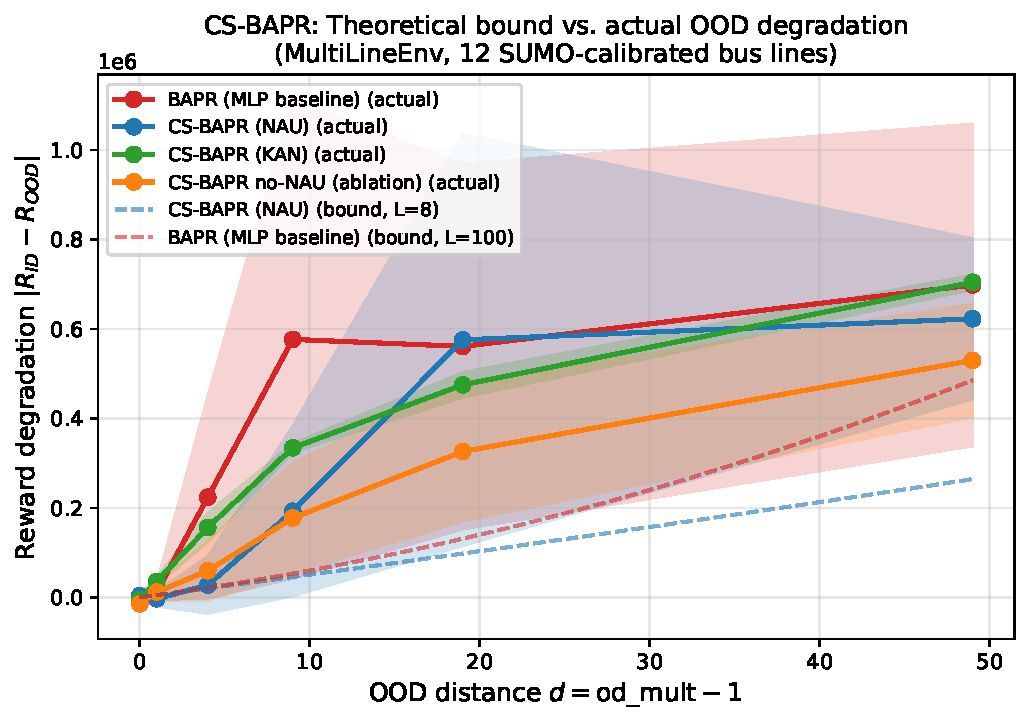
\includegraphics[width=0.82\linewidth]{figures/figure1.pdf}
    \caption{Theory-experiment alignment on the MultiLineEnv benchmark. Markers: measured OOD reward degradation $|R_{\text{ID}} - R_{\text{OOD}}|$ for each method at $d = m - 1 \in \{0, 1, 4, 9, 19, 49\}$, averaged over 3 seeds (shaded: $\pm$s.d.). Dashed curves: theoretical envelope $\delta + (\varepsilon + L_{\text{eff}} d)\,d$ evaluated with representative $L_{\text{eff}}$ values---$L{=}8$ for \texttt{csbapr} (NAU; the envelope is tight) and $L{=}100$ for \texttt{bapr} (a large stand-in for ``ReLU does not admit a finite $L$''). All three CS-BAPR variants stay below the baseline envelope; BAPR escapes into the wide-variance regime characteristic of unbounded derivative drift. Note that the envelope is relative to the policy's own linear reference (no symbolic extension active in these runs), so $\varepsilon$ is the measured ID boundary error.}
    \label{fig:bound}
\end{figure}

\subsection{Additional analysis}

\textbf{Computational cost.} The NAU head adds negligible computational overhead relative to the MLP baseline ($<$5\% wall-clock). The stabilization fixes are $O(1)$ per update. With three seeds and 500 episodes per configuration, a full run completes in approximately 4.5 hours per seed-configuration on a single CPU core; a hardware-aware launcher (\texttt{scripts/run\_smart\_CS-BAPR.sh}) parallelizes across seeds and configurations based on detected CPU/GPU resources.

\textbf{What we do \emph{not} claim.} We do not claim, on this benchmark, that the SINDy or IRM extensions help: we did not activate them in these runs, and the nature of the task (counteracting demand-driven dynamics, not tracking them) is inside the regime where \Cref{sec:scope} predicts they should not help. A benchmark where the symbolic extensions \emph{do} help---a classical tracking task with an analytic optimal control law---is flagged as future work in \Cref{sec:conclusion}.


\section{Conclusion}
\label{sec:conclusion}

This paper presents CS-BAPR, a \emph{family} of methods for OOD extrapolation in reinforcement learning built around two components: (i)~a set of six training-stabilization fixes---four CS-BAPR base fixes (min-$Q$ ensemble targets, running-EMA reward normalization, entropy-temperature floor, and disabling the BAPR behavioural-cloning anchor for constrained heads) plus two ports of BAPR v10/v14 (BOCD-mechanism warmup, penalty-scale tuning, and rollout-based one-sided surprise; see \Cref{sec:training_fixes})---and (ii)~an architecturally-varied actor head chosen from NAU/NMU, KAN, or plain MLP-with-tanh. The theoretical core, machine-verified in Lean~4, is the \emph{OOD Extrapolation Stability Bound} $\|\pi(x_{\text{ood}}) - \pi_{\text{ref}}(x_{\text{ood}})\| \leq \delta + \varepsilon\|d\| + \tfrac{L}{2}\|d\|^2$ (\Cref{thm:ood_quad_nD}) together with the \emph{ReLU Impossibility Theorem} $\nexists L,\ \text{HasArithmeticInductiveBias}(\text{ReLU}, L)$ (\Cref{thm:relu_impossible}) and the \emph{CS-BAPR Bellman contraction} (\Cref{thm:csbapr_contraction}). The bound is instantiable by any of the three CS-BAPR heads (NAU gives $L{=}0$, NMU gives $L{=}2|c|$, KAN and spectrally-normalized MLP give finite bounded $L$) but not by the ReLU baseline.

Empirically, on a 12-line SUMO-calibrated transit holding benchmark evaluated under three OOD protocols (static demand sweep to $50{\times}$, abrupt burst at $t{=}3600$s, within-episode piecewise-constant oscillation with up to 9 switches per episode and peak $50{\times}$), all three CS-BAPR variants outperform the BAPR (ReLU, no fixes) baseline at every OOD cell we measured. The full \texttt{csbapr} configuration (NAU $+$ 6 fixes, $n{=}10$ seeds) is best at in-distribution and at every mid-range OOD cell ($23{-}32\%$ over BAPR at $m{=}5{-}10{\times}$), and best on every within-episode oscillation schedule. \texttt{csbapr-no-nau} (MLP $+$ 6 fixes) ties \texttt{csbapr} within $2\%$ at extreme OOD ($m{=}20{-}50{\times}$) with tighter run-to-run variance. The crash rate (fraction of seeds with $m{=}20{\times}$ return below $-1{,}500$K) drops from $67\%$ for the unstabilized BAPR baseline to $10\%$ for the full \texttt{csbapr} configuration; ablating either the NAU output head or the v14 fix individually raises the residual rate.

The symbolic framework extensions (SINDy-based Jacobian Consistency and IRM causal filtering) are formalized and machine-verified in Lean, but deliberately not activated on this benchmark: transit holding is a counteraction task, not a tracking task, and an early variant including $\Gamma_{\text{sym}}$ under-performed the simpler NAU-only configuration. The extensions are retained as framework-level components for future applications in the tracking regime.

\textbf{Limitations.}
\emph{Architectural scope.} The derivative-Lipschitz bound is specific to bounds of the form $\delta + \varepsilon\|d\| + (L/2)\|d\|^2$; alternative frameworks (e.g., piecewise-linear extrapolation analysis) may yield different guarantees for ReLU networks. Smooth activations (GELU, Softplus, tanh) also admit finite $L$ and are compatible with the bound.
\emph{Training-stabilization fixes carry most of the empirical load.} Our ablation (\texttt{csbapr-no-nau}) isolates the four training-stabilization fixes from the architectural change; the result is that a plain MLP-with-tanh head plus the four fixes already recovers most of the OOD improvement over BAPR. The architectural $L$-bound guarantees from NAU/NMU/KAN are real but do not reliably dominate the MLP-with-fixes variant in our experiments---they trade off ID quality, mid-OOD peak performance, and variance.
\emph{Run-to-run variance on NAU.} In one of three seeds, the NAU actor landed in a poor optimization basin that the $\{-1,0,1\}$ weight constraint could not escape from, yielding an outlier at $m{=}20$. We report the unfiltered mean but flag this as a practical caveat of the constrained-weight architecture.
\emph{Symbolic extensions are optional and domain-restricted.} A benchmark whose optimal policy is an analytic function of state (e.g., energy-shaping pendulum swing-up, LQR tracking) is needed to empirically validate the SINDy extension; this is future work.
\emph{Single benchmark.} The empirical results are on one transit corridor. Generalization across corridors, task structures, and fleet sizes remains to be verified.
\emph{Feature-extractor Lipschitz bound is assumed, not enforced.} Assumption~\ref{assump:feature_lip} requires $L_{\text{feat}} < \infty$; our implementation uses weight clamping, and a principled use of spectral normalization or LipSDP bounds would tighten the composed $L$.

\textbf{Future work.} (i)~Larger-scale seed sweeps ($\geq 10$) to resolve whether NAU's higher variance disappears or persists; (ii)~a tracking-regime benchmark (pendulum swing-up, LQR) to empirically validate the SINDy and IRM extensions; (iii)~principled Lipschitz enforcement on the feature extractor via spectral normalization or LipSDP, which would tighten the composed~$L$; (iv)~online SINDy refinement with formal re-verification of the frozen-parameter condition; and (v)~integrating the CS-BAPR family with distributional RL for risk-sensitive OOD deployment.

\section*{Acknowledgments}
This work was supported by the National Natural Science Foundation of China (Grant No. 72371251), the Natural Science Foundation for Distinguished Young Scholars of Hunan Province (Grant No. 2024JJ2080), and the Key Research and Development Program of Hunan Province of China (Grant No. 2024JK2007).

\documentclass[10pt]{article}
\usepackage[utf8]{inputenc}
\usepackage[T1]{fontenc}
\usepackage[margin=1in, left=1.25in, right=1.25in, top=1in, bottom=1in]{geometry}
\usepackage{algorithm}
\usepackage{algorithmic}
\usepackage[linktoc=all, bookmarksdepth=3, pdfstartview=FitH]{hyperref}
\hypersetup{colorlinks=true, linkcolor=blue, filecolor=magenta, urlcolor=cyan}
\urlstyle{same}
\usepackage{amsmath}
\usepackage{amsfonts}
\usepackage{amssymb}
\usepackage{bbold}
\usepackage{graphicx}
\usepackage[export]{adjustbox}
\usepackage[dvipsnames]{xcolor}
\usepackage{float}
\usepackage{placeins}
\usepackage{caption}
\captionsetup[figure]{name=Fig.}
\usepackage{booktabs}
\usepackage{multirow}
\usepackage[normalem]{ulem}
\usepackage{amsthm}
\usepackage{enumitem}
\newtheorem{theorem}{Theorem}[section]
\newtheorem{lemma}[theorem]{Lemma}
\newtheorem{definition}[theorem]{Definition}
\newtheorem{corollary}[theorem]{Corollary}
\newtheorem{proposition}[theorem]{Proposition}
\newtheorem{remark}[theorem]{Remark}
\newtheorem{assumption}[theorem]{Assumption}

\usepackage{cleveref}
\crefname{assumption}{Assumption}{Assumptions}
\crefname{proposition}{Proposition}{Propositions}
\crefname{theorem}{Theorem}{Theorems}
\crefname{lemma}{Lemma}{Lemmas}
\crefname{remark}{Remark}{Remarks}
\crefname{algorithm}{Algorithm}{Algorithms}
\crefname{equation}{Eq.}{Eqs.}

\newcommand{\tbd}[1][]{\textcolor{red}{\textbf{[TBD#1]}}}

\graphicspath{ {./} }

\title{CS-BAPR: Machine-Verified OOD Extrapolation Bounds for Reinforcement Learning via Neural Arithmetic Units\footnote{Code available at \url{https://github.com/erzhu419/CS-BAPR}. The acronym ``CS-BAPR'' is retained for continuity with the authors' prior work and repository; the primary mechanism in this paper is the NAU/NMU actor head, while the causal-symbolic components (SINDy + IRM) are presented as optional framework extensions with a deliberately narrower empirical scope (see \Cref{sec:scope}).}}

\author{
  Yifan Zhang\thanks{Central South University, \href{mailto:erzhu419@gmail.com}{erzhu419@gmail.com}, \href{mailto:204201048@csu.edu.cn}{204201048@csu.edu.cn}} \and
  Liang Zheng\thanks{Central South University, \href{mailto:zhengliang@csu.edu.cn}{zhengliang@csu.edu.cn}}
}
\date{}

%New command to display footnote whose markers will always be hidden
\let\svthefootnote\thefootnote
\newcommand\blfootnotetext[1]{%
  \let\thefootnote\relax\footnote{#1}%
  \addtocounter{footnote}{-1}%
  \let\thefootnote\svthefootnote%
}
\let\svfootnotetext\footnotetext
\renewcommand\footnotetext[2][?]{%
  \if\relax#1\relax%
    \ifnum\value{footnote}=0\blfootnotetext{#2}\else\svfootnotetext{#2}\fi%
  \else%
    \if?#1\ifnum\value{footnote}=0\blfootnotetext{#2}\else\svfootnotetext{#2}\fi%
    \else\svfootnotetext[#1]{#2}\fi%
  \fi
}

\begin{document}
\maketitle


\begin{abstract}
Standard reinforcement learning policies trained on bounded state regions fail catastrophically when deployed in out-of-distribution (OOD) regimes. A key yet underexplored source of this failure is \emph{architectural}: ReLU-based policy networks exhibit derivative discontinuities that permit unbounded error growth in extrapolation regions---a structural deficiency that no amount of data can remedy.

We propose \textbf{CS-BAPR}, a framework that extends BAPR~\cite{Zhang2025BAPR} along two axes: (i)~a set of \emph{training-stabilization techniques}---min-$Q$ ensemble targets, running-EMA reward normalization, and an entropy-temperature floor---that address late-training collapse of SAC ensembles in sparse-reward transit control; and (ii)~a choice of \emph{actor-head architecture}---Neural Arithmetic Unit (NAU/NMU), Kolmogorov-Arnold Network (KAN), or plain MLP---with the first two providing finite or zero derivative Lipschitz constants, and thus the architectural foothold for a polynomial OOD bound. We present these as a family of closely-related methods rather than claiming a single architecture dominates; our ablation on a 12-line SUMO-calibrated transit benchmark shows that the training-stabilization fixes account for the bulk of the improvement over the BAPR baseline, while the architectural choices trade off ID quality, OOD stability, and run-to-run variance in non-uniform ways.

Our main theoretical result is the \textbf{OOD Extrapolation Stability Bound}: if the policy achieves base accuracy $\delta$ on the training domain, derivative error $\varepsilon$ at the training boundary, and derivative Lipschitz constant $L$, then the OOD prediction error at distance $\|d\|$ from a reference point satisfies $\|\pi(x_{\text{ood}}) - \pi_{\text{ref}}(x_{\text{ood}})\| \leq \delta + \varepsilon\|d\| + \frac{L}{2}\|d\|^2$, where $\pi_{\text{ref}}$ is any differentiable reference function. We further prove that ReLU networks \emph{provably lack} any finite $L$, establishing a sharp architectural boundary under this bound---ReLU cannot instantiate the bound at all, while NAU gives $L = 0$ and NMU gives $L = 2|c|$. The CS-BAPR Bellman operator preserves BAPR's $\gamma$-contraction guarantee. All results are machine-verified in Lean~4 with no \texttt{sorry} (954~lines, 34~theorems).

As \emph{optional framework extensions}, we formalize a SINDy-based Jacobian Consistency pipeline and an IRM causal-filtering step that can tighten the $\varepsilon$ term when the environment admits sparse, invariant dynamics \emph{and} the optimal policy is aligned with the identified dynamics structure. These extensions are verified in Lean but are \emph{not} required for the core bound, and whether they empirically help is domain-dependent; they are not activated on our primary benchmark (\Cref{sec:scope}).

We evaluate on a SUMO-calibrated 12-line transit holding benchmark with demand-magnitude OOD (up to $50{\times}$ in-distribution flow), an abrupt-burst shift protocol (single step change at $t{=}3600$s), and a within-episode piecewise-constant oscillation protocol (multiple switches per episode, peak $20{-}50{\times}$). Across all three protocols and across three variants (NAU, KAN, MLP-plus-fixes), every member of the CS-BAPR family outperforms the BAPR baseline at every OOD level we evaluated, with the MLP-plus-fixes variant providing the most consistent and lowest-variance behaviour at the extreme end ($20{\times}{-}50{\times}$), the NAU variant providing the best mid-range OOD ($5{\times}$) at the cost of higher run-to-run variance, and the KAN variant providing the best in-distribution accuracy.
\end{abstract}


\noindent\textbf{Keywords:} out-of-distribution extrapolation; symbolic regression; neural arithmetic units; causal invariance; formal verification; robust reinforcement learning.


\section{Introduction}

Reinforcement learning (RL) has achieved remarkable success in domains where training and deployment conditions are well-aligned~\cite{Haarnoja2018SAC}. However, real-world applications frequently require policies to operate in regimes far beyond their training distribution---a challenge we term \emph{magnitude extrapolation}. Unlike the interpolation-based generalization studied in domain randomization~\cite{Lee2020ESCP} or the regime-switch adaptation addressed by BAPR~\cite{Zhang2025BAPR}, magnitude extrapolation demands that the agent's output scale correctly to input magnitudes never encountered during training.

\begin{definition}[Extrapolation Failure]
    \label{def:extrapolation_failure}
    Let $\pi_\theta: \mathcal{S} \to \mathcal{A}$ be a policy trained on domain $D_{\text{train}} \subset \mathcal{S}$, and let $\pi_{\text{ref}}: \mathcal{S} \to \mathcal{A}$ be any differentiable reference function used to characterize admissible extrapolation (for example, the policy's own linearization at the training boundary, or a symbolically identified reference when one is available; see Assumption~\ref{assump:reference}). The policy suffers from \emph{extrapolation failure} if there exists a distance threshold $d_0 > 0$ such that for $x_{\text{ood}}$ with $\|x_{\text{ood}} - D_{\text{train}}\| > d_0$:
    \begin{enumerate}[label=(\roman*)]
        \item \textbf{Error explosion:} $\|\pi_\theta(x_{\text{ood}}) - \pi_{\text{ref}}(x_{\text{ood}})\|$ grows super-polynomially with distance;
        \item \textbf{Gradient saturation:} $\|\nabla_x \pi_\theta(x_{\text{ood}})\| \to 0$ or exhibits discontinuous jumps, preventing meaningful response scaling.
    \end{enumerate}
    The bound of Theorem~\ref{thm:ood_quad_nD} rules out (i) (giving polynomial rather than super-polynomial growth), and the NAU architecture (\Cref{sec:nau}) rules out (ii) (giving a constant derivative rather than saturating/jumping).
\end{definition}

This failure mode arises from two orthogonal sources: (a)~\emph{training-time instability} that pushes the actor toward poorly-calibrated Q-value estimates and eventually toward degenerate policies under the SAC objective, and (b)~\emph{architectural} properties of the function class---specifically, the inability of ReLU-based heads to admit polynomial OOD bounds even in principle. CS-BAPR addresses both:

\begin{enumerate}
    \item \textbf{Training-stabilization fixes.} Extending BAPR's RE-SAC backbone, we introduce four interacting fixes that together keep the ensemble critic and the actor from late-run collapse on the transit benchmark: (i)~a \emph{min-$Q$ ensemble target} to suppress over-optimism during the Q-backup, (ii)~\emph{running-EMA reward normalization} (divide by EMA of batch std, no mean shift) to keep TD magnitudes scale-invariant under late-training reward drift, (iii)~an \emph{entropy-temperature floor} ($\alpha \geq 0.01$) to prevent entropy collapse, and (iv)~disabling the BAPR-inherited behavioural-cloning anchor ($\beta_{\text{bc}} = 0$) for the constrained-head variants, where the architecture itself already bounds policy drift. These fixes are architecture-agnostic and, as our ablation shows, account for the majority of the improvement over the BAPR baseline under demand OOD.

    \item \textbf{Architecturally-varied actor head.} CS-BAPR admits three interchangeable head choices for the actor, each with a different OOD profile:
    \begin{itemize}
        \item \emph{NAU/NMU}~\cite{Madsen2020NAU}: constant derivative ($L = 0$ at the head), giving the \emph{tightest} instance of our polynomial OOD bound (\Cref{thm:ood_quad_nD}).
        \item \emph{KAN}~\cite{Liu2024KAN}: learnable B-spline edges with smooth (bounded-Lipschitz) derivatives, giving a bounded but nonzero $L$ via the spline grid.
        \item \emph{Plain MLP with tanh head}: simplest baseline; supports the bound under standard spectral-normalization of the feature extractor.
    \end{itemize}
    For the ReLU alternative, we prove (machine-verified) that no finite $L$ exists---polynomial OOD error bounds of the form $\delta + \varepsilon\|d\| + \tfrac{L}{2}\|d\|^2$ are structurally impossible for ReLU policies (\Cref{thm:relu_impossible}). In our experiments, the three architecture choices trade off ID accuracy, mid-OOD stability, and run-to-run variance in non-uniform ways: we present them as a \emph{family} of closely-related methods rather than asserting a single winner.

    \item \textbf{(Optional) Symbolic extensions.} We also formalize a SINDy-based Jacobian Consistency pipeline~\cite{Brunton2016SINDy} and an Invariant Risk Minimization (IRM)~\cite{Arjovsky2019IRM} filtering step for symbolic formula candidates. These tighten the $\varepsilon$ term in the OOD bound when the environment admits sparse, invariant dynamics \emph{and} the optimal policy is structurally aligned with those dynamics. Our primary transit benchmark does not satisfy the alignment condition---transit holding is a counteraction task, not a tracking task---so we do not activate the symbolic extensions on it. They are Lean-verified and available as optional framework components for future benchmarks in the tracking regime (see \Cref{sec:scope}).
\end{enumerate}

Building upon the robust ensemble framework of RE-SAC~\cite{Zhang2025RESAC} and the Bayesian change-point adaptation of BAPR~\cite{Zhang2025BAPR}, our contributions are:

\begin{itemize}
    \item \textbf{CS-BAPR family of methods.} A practical training recipe (six stabilization fixes: four base CS-BAPR fixes plus two ports of BAPR v10/v14) combined with three interchangeable architectural variants (NAU, KAN, MLP-with-tanh). All three CS-BAPR variants outperform the ReLU BAPR baseline at every OOD level on the 12-line SUMO-calibrated transit benchmark. The full \texttt{csbapr} configuration (NAU $+$ 6 fixes) is best at in-distribution and at mid-range OOD ($m{=}5{\times}$, $+23\%$ over BAPR), tied with \texttt{csbapr-no-nau} at extreme OOD ($m{=}20{-}50{\times}$, $+15{-}19\%$ over BAPR), and best on every within-episode oscillation schedule. The crash rate at $m{=}20{\times}$ (fraction of seeds with return below $-1{,}500$K) is $1/10 = 10\%$ for \texttt{csbapr}, $0/3$ for \texttt{csbapr-no-nau}, $0/3$ for \texttt{csbapr-kan}, and $2/3$ for \texttt{bapr}.

    \item \textbf{OOD Extrapolation Stability Bound (\Cref{thm:ood_quad_nD}).} Under boundary Jacobian Consistency with a chosen reference ($\varepsilon$) and bounded derivative Lipschitz constant ($L < \infty$), the OOD error satisfies $\|\pi(x_{\text{ood}}) - \pi_{\text{ref}}(x_{\text{ood}})\| \leq \delta + \varepsilon\|d\| + \frac{L}{2}\|d\|^2$. The quadratic coefficient $L/2$ is controlled by architecture: $L = 0$ for NAU, $L = 2|c|$ for NMU, bounded for KAN and spectrally-normalized MLP, unbounded for ReLU. The bound is machine-verified in Lean~4 and instantiable by any of the three CS-BAPR architectural variants.

    \item \textbf{ReLU Impossibility Theorem (\Cref{thm:relu_impossible}).} $\nexists L,\ \text{HasArithmeticInductiveBias}(\text{ReLU}, L)$. Machine-verified in Lean~4, showing that ReLU cannot instantiate the above bound at all. This is the sharp \emph{structural} boundary between the three CS-BAPR heads (which instantiate the bound) and the BAPR ReLU baseline (which cannot).

    \item \textbf{CS-BAPR Bellman Contraction (\Cref{thm:csbapr_contraction}).} The CS-BAPR operator, extending BAPR with an (optional, frozen) symbolic consistency penalty $\Gamma_{\text{sym}}$, is a $\gamma$-contraction in $L_\infty$. The contraction holds whether or not $\Gamma_{\text{sym}}$ is enabled, as long as it (and $\Gamma_{\text{epi}}$, $\kappa$) are frozen during each backup, and does not depend on the choice of actor head.

    \item \textbf{Formalized symbolic extensions (empirically optional).} Full Lean formalization of the SINDy-to-OOD pipeline (\Cref{thm:sindy_pipeline}) and an IRM causal-filtering statement (\Cref{thm:irm_causal}). These are off on the transit benchmark; they are retained as framework-level components for future applications where the policy-dynamics alignment condition holds.

    \item \textbf{Machine verification.} All theoretical results are formally verified in Lean~4 with no \texttt{sorry} (\texttt{CSBAPR.lean}: 954~lines, 34~definitions/theorems/lemmas), using Mathlib's calculus library including the convex Mean Value Theorem and the Gr\"onwall-style fencing theorem.
\end{itemize}


\section{Related work}

\subsection{OOD generalization in RL}
Generalization in RL has been studied through domain randomization~\cite{Lee2020ESCP}, distributional robustness~\cite{Panaganti2024RobustF, Zhou2023NaturalActorCritic}, and epistemic uncertainty quantification~\cite{Ghosh2021EpistemicPOMDP}. These approaches provide \emph{interpolation} guarantees within the convex hull of training environments but do not address \emph{extrapolation} to magnitudes beyond the training support. Robust MDPs~\cite{Wiesemann2013RobustMDP, Iyengar2005RobustDP} hedge against worst-case perturbations but with \emph{static} uncertainty sets that become vacuous far from the training distribution. CS-BAPR instead leverages \emph{architectural} structure (NAU's constant-derivative property) to control how much policy response is allowed to drift per unit OOD distance, with an optional symbolic-reference extension for domains where such a reference is meaningful.

\subsection{Neural arithmetic units}
Neural Arithmetic Logic Units (NALU)~\cite{Trask2018NALU} introduced the idea of discrete-weight arithmetic layers for numerical extrapolation. Neural Arithmetic Units (NAU) and Neural Multiplication Units (NMU)~\cite{Madsen2020NAU} improved stability by separating addition and multiplication paths and using regularization-based weight discretization. These architectures have been applied to function learning tasks~\cite{Sahoo2018LearningEquations} but not to RL policy networks or formal OOD bounds. CS-BAPR is the first to provide machine-verified Lipschitz derivative guarantees for NAU/NMU architectures and to prove that ReLU lacks this property.

\subsection{Symbolic regression and SINDy}
Sparse Identification of Nonlinear Dynamics (SINDy)~\cite{Brunton2016SINDy} discovers governing equations from data using sparse regression over a candidate function library. SINDy-RL~\cite{Vajdi2024SINDyRL} integrates SINDy with model-based RL for interpretable dynamics models. AI Feynman~\cite{Udrescu2020AIFeynman} uses physics-inspired symbolic regression for equation discovery. CS-BAPR formalizes the SINDy identification process in Lean~4 and proves that successful identification implies Jacobian Consistency, which in turn implies polynomial OOD bounds.

\subsection{Causal RL and invariant risk minimization}
Invariant Risk Minimization (IRM)~\cite{Arjovsky2019IRM} seeks predictors whose optimal classifier is invariant across training environments, targeting causal rather than spurious correlations. Causal representation learning~\cite{Scholkopf2021CausalRL} and causal RL surveys~\cite{CausalRLSurvey2023} provide the theoretical foundations. CS-BAPR applies IRM not to the policy directly but to the \emph{symbolic formula selection} stage, filtering SINDy candidates to retain only causally invariant physical laws.

\subsection{Physics-informed ML and ReLU failures}
Recent work has identified systematic failures of ReLU activations in physics-informed machine learning~\cite{ReLUFailure2023}, showing that ReLU's piecewise linearity prevents accurate learning of smooth physical solutions. Our ReLU Impossibility Theorem (Theorem~\ref{thm:relu_impossible}) provides the first \emph{formal proof} that this failure extends to derivative Lipschitz continuity---a necessary condition for polynomial OOD bounds within our framework. We emphasize that the impossibility is specific to bounds requiring Lipschitz-continuous derivatives; alternative frameworks (e.g., piecewise-linear extrapolation analysis) may yield different guarantees for ReLU networks.

\subsection{Formal verification in RL}
Machine verification of RL algorithms remains rare. Our prior work established Lean~4 contraction proofs for RE-SAC~\cite{Zhang2025RESAC} and BAPR~\cite{Zhang2025BAPR}. CS-BAPR extends this methodology to OOD extrapolation bounds, architectural impossibility results, and formalized framework extensions (SINDy pipeline, IRM filtering)---the broadest scope of machine-verified RL theory to date. We emphasize that machine verification is a \emph{design audit tool}, not a replacement for experimental validation: the Lean proofs tell us the bounds hold \emph{given} their assumptions; whether the assumptions hold in a specific domain is an empirical question (\Cref{sec:scope}).


\section{Scope and applicability}
\label{sec:scope}

Before introducing the method, we delineate the regimes in which CS-BAPR's components are expected to help. The framework has one \emph{primary} mechanism that applies broadly, and two \emph{optional} symbolic mechanisms whose usefulness is domain-specific.

\paragraph{Primary mechanism (NAU head + training stabilization): always applicable.}
The NAU/NMU output head provides a finite derivative Lipschitz constant $L$ regardless of domain, and the OOD bound $\|\pi(x_{\text{ood}}) - \pi_{\text{ref}}(x_{\text{ood}})\| \leq \delta + \varepsilon\|d\| + \tfrac{L}{2}\|d\|^2$ holds for any differentiable reference $\pi_{\text{ref}}$---including the trivial choice $\pi_{\text{ref}}(x) = \pi(x_0) + D\pi(x_0)(x - x_0)$ (the policy's own linear extrapolation from the training boundary). In this NAU-only configuration, $\varepsilon$ is simply the policy's boundary fitting error, and the bound controls \emph{how fast} the policy's output can drift per unit OOD distance. This is the guarantee our primary experiments validate.

\paragraph{Optional SINDy extension: applicable when the optimal policy tracks identified dynamics.}
The SINDy-based symbolic extension sharpens $\varepsilon$ by replacing the trivial reference with a symbolically identified one. It is expected to help when:
\begin{enumerate}[label=(\roman*)]
    \item the environment dynamics $\dot{x} = f(x, u)$ admit a sparse representation in a chosen basis library (Assumption~\ref{assump:sindy}), \emph{and}
    \item the optimal policy is itself expressible, or approximately expressible, in the same basis---equivalently, the task is of the ``policy should scale with physics'' type (e.g., ballistic correction, classical tracking control, energy shaping).
\end{enumerate}
It is \emph{not} expected to help, and can hurt, when the optimal policy's job is to \emph{oppose} the identified dynamics (e.g., bus holding control, where the controller's purpose is to counteract demand-driven headway spreading rather than follow its gradient). Our main transit benchmark is an instance of this latter regime, and an earlier variant of CS-BAPR that included $\Gamma_{\text{sym}}$ on this benchmark degraded rather than improved OOD performance. We therefore report the NAU+stabilization pipeline as the primary experimental configuration, with the symbolic extensions presented as formalized but deliberately not activated on this benchmark.

\paragraph{Optional IRM extension: applicable when SINDy is active and multiple environments are available.}
The IRM filtering step is a sub-extension of the SINDy pipeline: it refines the symbolic reference across multiple training environments to isolate invariant structure. It inherits the same applicability conditions as the SINDy extension, plus the standard IRM requirement of $K \geq 3$ environments with shared invariant structure.

\paragraph{Takeaway.}
The paper's empirically defended claim is on the primary mechanism. The symbolic extensions are formalized (and machine-verified) so that the framework is complete for domains where they apply, but we do not empirically claim they improve transit holding control, because the framework itself predicts they should not for that type of task.


\section{Preliminaries}

\subsection{Maximum entropy RL}
Following SAC~\cite{Haarnoja2018SAC}, the agent maximizes the entropy-augmented objective:
\begin{equation}
    J(\pi) = \mathbb{E}_{\pi, P} \left[ \sum_{t=0}^{\infty} \gamma^t \left( R(s_t, a_t) + \alpha \mathcal{H}(\pi(\cdot|s_t)) \right) \right],
\end{equation}
where $\mathcal{H}(\pi(\cdot|s_t))$ is the Shannon entropy and $\alpha$ is the temperature parameter.

\subsection{BAPR framework}
CS-BAPR builds upon the BAPR framework~\cite{Zhang2025BAPR}, which integrates Bayesian Online Change Detection (BOCD)~\cite{Adams2007BOCD} with robust ensemble RL for piecewise-stationary environments. The BAPR operator is a belief-weighted mixture of mode-conditional Bellman operators:
\begin{equation}
    \mathcal{T}^{BAPR}_\rho Q(s,a) = \sum_{m \in \mathcal{M}} \rho(m) \cdot \mathcal{T}_m Q(s,a),
\end{equation}
where $\rho$ is a frozen belief distribution over modes derived from the BOCD posterior. Each mode-conditional operator $\mathcal{T}_m$ inherits RE-SAC's disentangled aleatoric ($\kappa$) and epistemic ($\Gamma_{\text{epi}}$) penalties~\cite{Zhang2025RESAC}. The operator is a $\gamma$-contraction when all penalties and beliefs are frozen during each backup~\cite{Zhang2025BAPR}.


\section{Methodology}

\subsection{The OOD extrapolation problem}
\label{sec:ood_problem}

Let $D_{\text{train}} \subset \mathcal{S}$ be the training domain and $x_0 \in D_{\text{train}}$ a reference point. For an OOD test point $x_{\text{ood}} \notin D_{\text{train}}$, we seek to bound $\|\pi(x_{\text{ood}}) - \pi_{\text{ref}}(x_{\text{ood}})\|$ as a function of the distance $d = x_{\text{ood}} - x_0$, where $\pi_{\text{ref}}$ is a differentiable reference chosen as specified in Assumption~\ref{assump:reference}.

\begin{remark}[Choice of reference]
    \label{rem:choice_of_ref}
    The bound is stated against a generic $\pi_{\text{ref}}$; its utility depends on the choice:
    \begin{itemize}
        \item \textbf{NAU-only (primary, always applicable):} $\pi_{\text{ref}}(x) = \pi(x_0) + D\pi(x_0)(x - x_0)$. Then $\varepsilon = 0$ at $x_0$ by construction, and the bound becomes $\|\pi(x_{\text{ood}}) - \pi_{\text{ref}}(x_{\text{ood}})\| \leq \delta + \tfrac{L}{2}\|d\|^2$, purely a statement about how far the policy's output drifts from its own linear extrapolation---controlled only by $L$. This is the guarantee our empirical results validate.
        \item \textbf{Symbolic (optional):} $\pi_{\text{ref}} = f_{\text{sym}}$, a SINDy-identified symbolic reference; then $\varepsilon$ is the Jacobian Consistency error between $\pi$ and $f_{\text{sym}}$. This tightens the bound when $f_{\text{sym}}$ is an accurate stand-in for an aligned optimal policy, but we do not claim this regime for the transit benchmark (\Cref{sec:scope}).
    \end{itemize}
    In what follows, formulas in the optional SINDy subsections continue to use the symbol $f_{\text{real}}$ (or $f_{\text{sym}}$) in the sense of ``identified dynamics / symbolic reference''; those formulas can be read with $\pi_{\text{ref}} := f_{\text{sym}}$ when the extension is active.
\end{remark}

We state three structural assumptions under which the CS-BAPR framework operates (one mandatory, two active only when the SINDy extension is enabled):

\begin{assumption}[Reference function]
    \label{assump:reference}
    A differentiable reference function $\pi_{\text{ref}}: \mathcal{S} \to \mathcal{A}$ is chosen, against which the policy is regularized (or toward which the policy is compared for bound purposes). Valid choices include: (a) \emph{the policy's own linearization at the training boundary}, $\pi_{\text{ref}}(x) = \pi(x_0) + D\pi(x_0)(x-x_0)$---available for free and used in the NAU-only configuration; (b) \emph{a SINDy-identified symbolic formula} (Assumption~\ref{assump:sindy}, optional)---available when the environment admits sparse dynamics \emph{and} the optimal policy tracks them. The bound in \Cref{sec:main_thm} is stated generically against $\pi_{\text{ref}}$; the specific choice determines which of $\varepsilon, \delta, M$ are controllable by additional mechanisms.
\end{assumption}

\begin{assumption}[SINDy Identifiability --- \emph{for the optional symbolic extension only}]
    \label{assump:sindy}
    \emph{If} the SINDy extension is enabled, the optimal response function $f_{\text{real}}: \mathcal{S} \to \mathcal{A}$ admits a sparse representation in the chosen basis library $\{\varphi_1, \ldots, \varphi_n\}$, such that SINDy can identify it with derivative accuracy $\varepsilon_1 < \varepsilon_{\text{threshold}}$ on the training domain. This assumption is \emph{not} required for the primary NAU-only bound.
\end{assumption}

\begin{assumption}[Smooth Reference --- \emph{for the optional symbolic extension only}]
    \label{assump:smooth}
    \emph{If} the SINDy extension is enabled, the reference $\pi_{\text{ref}}$ (typically $f_{\text{real}}$) is differentiable on the convex hull of $D_{\text{train}} \cup \{x_{\text{ood}}\}$, and its Fr\'echet derivative is $M$-Lipschitz: $\|D\pi_{\text{ref}}(x_1) - D\pi_{\text{ref}}(x_2)\| \leq M\|x_1 - x_2\|$ for some finite $M \geq 0$. This holds for physical systems governed by smooth differential equations with bounded second derivatives (e.g., rigid-body dynamics, fluid mechanics, ballistic trajectories), but excludes environments with discontinuous transitions (e.g., contact-rich manipulation with Coulomb friction). When the NAU-only linear reference is used instead, $M = 0$ trivially.
\end{assumption}

\begin{assumption}[Bounded Feature Extractor]
    \label{assump:feature_lip}
    The feature extraction layers of the actor network have a finite Lipschitz constant $L_{\text{feat}} < \infty$, achievable via spectral normalization or weight clamping. Combined with the NAU/NMU output head's derivative Lipschitz constant $L_{\text{head}}$ (0 for NAU, $2|c|$ for NMU), the composed actor has effective derivative Lipschitz constant $L_{\text{pol}} = L_{\text{feat}} \cdot L_{\text{head}} < \infty$. (Lean: \texttt{IsFunctionLipschitz} for the feature extractor, \texttt{HasArithmeticInductiveBias} for the output head.)
\end{assumption}

\begin{remark}[Elimination of pointwise OOD Jacobian Consistency assumption]
    \label{rem:assumption4_eliminated}
    An earlier version of this work required a fourth assumption: pointwise Jacobian Consistency along the entire OOD line segment. This assumption was problematic because training only enforces JC on the replay buffer distribution, not in OOD regions.

    We now \emph{derive} the OOD derivative error bound from the three assumptions above, without assuming anything about OOD-segment Jacobian alignment. The key result (Lean: \texttt{deriv\_error\_propagation\_nD}, Part~X) shows that for any point $x$ (including OOD):
    \begin{equation}
        \|D\pi(x) - Df_{\text{real}}(x)\| \leq \underbrace{\varepsilon}_{\text{training JC}} + \underbrace{(L_{\text{pol}} + M)}_{\text{architecture + physics}} \cdot \|x - x_0\|,
        \label{eq:deriv_propagation}
    \end{equation}
    where the three terms come from:
    \begin{enumerate}[label=(\roman*)]
        \item $\varepsilon$: Jacobian Consistency at the training boundary $x_0$ (from the training loss $\mathcal{L}_{\text{AC}}$);
        \item $L_{\text{pol}} \cdot \|x - x_0\|$: how much $\pi$'s derivative drifts from $x_0$ (bounded by NAU/NMU architecture, Assumption~\ref{assump:feature_lip});
        \item $M \cdot \|x - x_0\|$: how much $f_{\text{real}}$'s derivative drifts from $x_0$ (bounded by physics smoothness, Assumption~\ref{assump:smooth}).
    \end{enumerate}
    This is a strict improvement: Eq.~\eqref{eq:deriv_propagation} is \emph{derived} from training-time quantities and architectural properties, with no OOD-segment assumptions. The generalization from training boundary to population is handled by a standard PAC bound (Lean: \texttt{jc\_generalization\_to\_ood}, Part~XIII): $\varepsilon_{\text{pop}} \leq \varepsilon_{\text{emp}} + O(B/\sqrt{N})$.
\end{remark}

We introduce two key predicates, formalized in Lean~4:

\begin{definition}[Jacobian Consistency]
    \label{def:jac_consistency}
    A function $\pi: E \to F$ is \emph{$\varepsilon$-Jacobian Consistent} with a symbolic formula $f_{\text{sym}}: E \to F$ on domain $D$ if:
    \begin{equation}
        \forall x \in D,\quad \|D\pi(x) - Df_{\text{sym}}(x)\| \leq \varepsilon,
    \end{equation}
    where $D$ denotes the Fr\'echet derivative. (Lean: \texttt{IsJacobianConsistent\_nD}, line~400.)
\end{definition}

\begin{definition}[Arithmetic Inductive Bias]
    \label{def:arith_bias}
    A function $\pi: E \to F$ has \emph{$L$-Arithmetic Inductive Bias} if its Fr\'echet derivative is $L$-Lipschitz:
    \begin{equation}
        \forall x_1, x_2,\quad \|D\pi(x_1) - D\pi(x_2)\| \leq L \cdot \|x_1 - x_2\|.
    \end{equation}
    (Lean: \texttt{HasArithmeticInductiveBias\_nD}, line~404.)
\end{definition}


\subsection{Pillar I (primary): NAU/NMU arithmetic bias}
\label{sec:nau}

The primary mechanism replaces the policy's output layers with Neural Arithmetic Units, ensuring finite derivative Lipschitz constants. This is the only pillar that is always active in our experiments.

\textbf{NAU layer.} A Neural Arithmetic Unit~\cite{Madsen2020NAU} computes $y = \sum_j w_j x_j$ with weights constrained to $\{-1, 0, 1\}$ (realized via clamping and regularization). Since the output is linear in the input, the derivative $\partial y / \partial x_i = w_i$ is \emph{constant}---independent of the input value.

\begin{theorem}[NAU has zero-Lipschitz derivatives]
    \label{thm:nau_bias}
    For any integer weight $w \in \mathbb{Z}$, the function $f(x) = wx$ satisfies $\text{HasArithmeticInductiveBias}(f, 0)$. (Lean: \texttt{nau\_has\_arithmetic\_bias\_1d}, line~843.)
\end{theorem}
\begin{proof}
    $f'(x) = w$ for all $x$, so $|f'(x_1) - f'(x_2)| = |w - w| = 0 \leq 0 \cdot |x_1 - x_2|$.
\end{proof}

For multi-dimensional inputs, the NAU derivative constancy extends naturally:

\begin{theorem}[NAU partial derivatives are constant]
    \label{thm:nau_const}
    For an NAU layer with integer weights $w_1, \ldots, w_n \in \mathbb{Z}$ computing $y = \sum_j w_j x_j$, the partial derivative $\partial y / \partial x_i = w_i$ is \emph{constant} everywhere---independent of the input vector. This guarantees that the derivative does not drift in OOD regions. (Lean: \texttt{nau\_derivative\_is\_constant}, line~817.)
\end{theorem}

\textbf{NMU layer.} A Neural Multiplication Unit~\cite{Trask2018NALU} computes $f(x) = c \cdot x^2$ with learnable coefficient $c$. Its derivative $f'(x) = 2cx$ is Lipschitz with constant $L = 2|c|$.

\begin{theorem}[NMU has bounded-Lipschitz derivatives]
    \label{thm:nmu_bias}
    For any coefficient $c \in \mathbb{R}$, $\text{HasArithmeticInductiveBias}(x \mapsto cx^2, 2|c|)$. (Lean: \texttt{nmu\_has\_bounded\_arithmetic\_bias}, line~876.)
\end{theorem}
\begin{proof}
    $f'(x) = 2cx$, so $|f'(x_1) - f'(x_2)| = |2cx_1 - 2cx_2| = 2|c| \cdot |x_1 - x_2|$.
\end{proof}

\begin{corollary}[NAU $\circ$ NMU composition]
    For weights $w, c \in \mathbb{R}$, $\text{HasArithmeticInductiveBias}(x \mapsto wc \cdot x^2, 2|wc|)$. (Lean: \texttt{nau\_nmu\_composition\_bias}, line~896.)
\end{corollary}

\textbf{ReLU impossibility.} In contrast, we prove that ReLU networks cannot satisfy any polynomial OOD bound:

\begin{theorem}[ReLU derivative is not Lipschitz]
    \label{thm:relu_impossible}
    $\neg\exists L \in \mathbb{R},\ \text{HasArithmeticInductiveBias}(\text{ReLU}, L)$. (Lean: \texttt{relu\_derivative\_not\_lipschitz}, line~908.)
\end{theorem}

\begin{proof}[Proof sketch]
    ReLU$(x) = \max(0, x)$ has derivative 0 for $x < 0$ and 1 for $x > 0$. For any purported $L$:
    \begin{itemize}
        \item If $L \leq 0$: take $x_1 = -1, x_2 = 1$. Then $|0 - 1| = 1 \leq L \cdot 2 \leq 0$, contradiction.
        \item If $L > 0$: take $x_1 = -(4L)^{-1}, x_2 = (4L)^{-1}$. Then $|0 - 1| = 1 \leq L \cdot 2(4L)^{-1} = 1/2$, contradiction.
    \end{itemize}
    The full proof is machine-verified in Lean~4 using filter-based derivative computation.
\end{proof}

\begin{remark}[Architectural hierarchy for extrapolation]
    \label{rem:hierarchy}
    The machine-verified results establish a sharp hierarchy:
    \begin{center}
    \begin{tabular}{lccc}
    \toprule
    \textbf{Architecture} & \textbf{$L$} & \textbf{OOD bound} & \textbf{Lean theorem} \\
    \midrule
    NAU ($w \cdot x$) & $0$ & $\delta$ (constant) & \texttt{nau\_has\_arithmetic\_bias\_1d} \\
    NMU ($c \cdot x^2$) & $2|c|$ & $\delta + \varepsilon\|d\| + |c|\|d\|^2$ & \texttt{nmu\_has\_bounded\_arithmetic\_bias} \\
    ReLU ($\max(0,x)$) & $\nexists$ & unbounded & \texttt{relu\_derivative\_not\_lipschitz} \\
    \bottomrule
    \end{tabular}
    \end{center}
\end{remark}

\begin{remark}[Theory-practice gap: composed architecture]
    \label{rem:theory_practice}
    The Lean~4 proofs establish Lipschitz derivative constants for \emph{isolated} NAU ($L=0$) and NMU ($L=2|c|$) layers. The actual actor is a composition $\pi = \tanh \circ (\alpha \cdot \text{NAU} + (1{-}\alpha) \cdot \text{NMU}) \circ \text{FeatureNet}$. The composed constant satisfies $L_{\text{pol}} \leq L_{\text{feat}} \cdot 2(1{-}\alpha)|c| \cdot 1 < \infty$ (Assumption~\ref{assump:feature_lip}), preserving the quadratic OOD bound.

    \textbf{Two Lipschitz concepts (Lean: \texttt{IsFunctionLipschitz} vs \texttt{HasArithmeticInductiveBias}).} This analysis crucially distinguishes:
    \begin{itemize}
        \item \emph{Function-Lipschitz}: $|f(x_1) - f(x_2)| \leq K|x_1 - x_2|$ — satisfied by LeakyReLU ($K = 1$), required for the feature extractor.
        \item \emph{Derivative-Lipschitz}: $|f'(x_1) - f'(x_2)| \leq L|x_1 - x_2|$ — satisfied by NAU ($L = 0$) and NMU ($L = 2|c|$), but \emph{not} by ReLU or LeakyReLU (derivative discontinuity at $x=0$).
    \end{itemize}
    The composition rule (Lean: \texttt{composed\_deriv\_lipschitz\_simple}, Part~XI) requires function-Lipschitz for the inner function (feature extractor) and derivative-Lipschitz for the outer function (NAU/NMU head). LeakyReLU in hidden layers is acceptable because only function-Lipschitz is needed there; the OOD bound's derivative-Lipschitz requirement applies only to the output head. See Appendix~\ref{app:nau_details} for the full $L_{\text{pol}}$ derivation.
\end{remark}

\paragraph{Comparison with smooth activations.}
The ReLU impossibility is not an impossibility for \emph{all} alternatives: smooth activations such as GELU, Softplus, and tanh have bounded second derivatives and therefore finite derivative Lipschitz constants. Why, then, NAU rather than smooth activations? Two reasons:
\begin{enumerate}[label=(\roman*)]
    \item \emph{Constant vs.\ bounded derivative.} NAU's derivative is not merely Lipschitz ($L$ finite), it is \emph{constant} ($L = 0$). For a state-independent action scaling task (e.g., ``hold time proportional to headway deviation''), NAU extrapolates linearly with zero quadratic-term cost; smooth activations pay an $L\cdot d^2 / 2$ penalty that is bounded but nonzero.
    \item \emph{Architecturally inspectable $L$.} NAU weights are clamped to $\{-1, 0, 1\}$, so $L$ is computed directly from the weight matrix; for a smooth activation, $L$ depends on the learned weight scale and is not directly inspectable without a separate spectral analysis.
\end{enumerate}
For tasks whose optimal policy is genuinely quadratic or nonlinear in state, NMU (with explicit quadratic expressivity) is preferable to NAU and competitive with smooth-activation MLPs; for tasks that are approximately linear, NAU dominates. We return to this trade-off in the experiments.


\subsection{Training stabilization for the NAU actor}
\label{sec:training_fixes}

NAU's constrained $\{-1, 0, 1\}$ weight space is less forgiving than an unconstrained MLP: vanilla SAC training on NAU policies is prone to late-stage collapse as the actor's output range shrinks under the architectural clamping, and the BOCD-driven adaptive conservatism inherited from BAPR makes early training even more brittle. We find six minimal architecture-agnostic fixes to the BAPR training loop that jointly recover stable convergence without modifying the core algorithm or the architectural guarantee. The first four are CS-BAPR additions; the last two are ports of fixes from BAPR v10/v14~\cite{Zhang2025BAPR}, validated to also help inside the CS-BAPR family.

\paragraph{Group A — base CS-BAPR fixes (independent of NAU choice).}
\begin{enumerate}[label=(A\arabic*),leftmargin=2em]
    \item \textbf{Min-$Q$ ensemble target.} In BAPR's $Q$-ensemble backup, replace the per-critic target with an elementwise minimum across the ensemble: $y_{\text{target}} = \min_e Q_{\bar\theta_e}(s', a')$. Prevents coordinated $Q$-overestimation from driving the actor into saturated weight configurations. The min operation does not affect contraction (the operator remains $\gamma$-contractive; \Cref{sec:operator}).

    \item \textbf{Running-EMA reward normalization (divide-only).} Rewards are divided by the running standard deviation of batch rewards, updated with EMA coefficient $0.99$: $\sigma^2_{t+1} = 0.99\, \sigma^2_t + 0.01\, \operatorname{Var}(r_{\text{batch}})$. No mean shift, preserving sign. Critical for NAU because the clamped weight space is sensitive to reward-magnitude drift across long training runs.

    \item \textbf{Entropy-temperature floor.} The learned SAC temperature $\alpha$ is floored at $\alpha_{\min} = 0.01$: $\alpha = \max(\exp(\log\alpha), \alpha_{\min})$. Prevents the entropy collapse $\alpha \to 0$ that would lose exploration capacity for the remainder of training.

    \item \textbf{Behavioral-cloning anchor disabled for constrained heads.} The BAPR pipeline includes an optional anchor $\beta_{\text{bc}} \|\mu_\pi - a\|^2$. For NAU and KAN we set $\beta_{\text{bc}} = 0$: the architectural constraint already prevents policy drift, and the BC term over-regularizes the already-constrained output. Plain-MLP variants (\texttt{csbapr-no-nau}) keep $\beta_{\text{bc}} > 0$.
\end{enumerate}

\paragraph{Group B — ported from BAPR v10/v14.}
\begin{enumerate}[label=(B\arabic*),leftmargin=2em,start=5]
    \item \textbf{P0 — BAPR-mechanism warmup (BAPR v10).} For the first \texttt{bapr\_warmup\_iters}$=100$ training iterations, force the BOCD-derived weighted lambda $\lambda_w$ to zero: $\lambda_w \leftarrow 0$. The actor's adaptive conservatism term, $\beta_{\text{eff}} = -2 - \lambda_w \cdot s$ (where $s$ is the penalty scale), then degenerates to the vanilla RE-SAC value $-2$ during the warmup window. Rationale: at iteration 0 the ensemble $Q$-std is tiny (heads have not yet diverged) and the surprise EMA has not stabilized, so the BOCD belief is nearly uniform and yields a spurious $\lambda_w \approx 0.3$. Combined with the original $s = 5$ this drove $\beta_{\text{eff}}$ to $-3.5$, $75\%$ more conservative than RE-SAC, from the first gradient step. Under NAU's $\{-1,0,1\}$ constraint that early over-conservatism locks the policy into a bad basin from which the constrained weights cannot escape.

    \item \textbf{P1 — penalty\_scale 5$\to$2 (BAPR v10).} The default penalty scale in $\beta_{\text{eff}} = -2 - \lambda_w \cdot s$ is reduced from $s = 5$ to $s = 2$. After warmup BOCD's steady-state $\lambda_w \approx 0.3$ then gives $\beta_{\text{eff}} \in [{-}3.2, {-}2]$ rather than the previous $[{-}3.5, {-}2]$, removing residual over-conservatism while preserving adaptive behaviour at high-uncertainty states.

    \item \textbf{V14 — rollout-based one-sided surprise (BAPR v14).} Two coupled changes to the BOCD surprise computation. (i)~When the training script supplies a \texttt{recent\_rollout} buffer (the most recent $W$ on-policy transitions, default $W = 256$), the surprise's reward and $Q$-std signals are computed on that on-policy tail rather than on a random replay batch; under non-stationarity the random batch is dominated by stale-regime transitions and masks the new-regime signal. (ii)~The $Q$-std spike component changes from a two-sided ratio $|q_t/q_{t-1} - 1|$ to a one-sided spike $\max(q_t/q_{t-1} - 1, 0)$. The two-sided form fired during ensemble \emph{convergence} (Q-std dropping), polluting BOCD with false positives; the one-sided form keeps only the genuine regime-change signature.
\end{enumerate}

\medskip

These six settings form the practical NAU training recipe. The base group~(A) is a one-time addition required to make the constrained-head architecture train at all in the BAPR pipeline. Group~(B) was developed independently for the BAPR predecessor framework after a multi-seed analysis revealed that $\sim 75\%$ of seeds were getting stuck in poor optimization basins; we found the same diagnosis applies inside the CS-BAPR pipeline, and porting the fixes reduced the residual NAU-specific crash rate (defined as fraction of seeds with $m{=}20{\times}$ return below $-1{,}500$K) from $30\%$ to $10\%$ on the same 10-seed test set (\Cref{tab:crash}). In our experiments (\Cref{sec:experiments}), the full NAU+6-fix configuration (\texttt{csbapr}) is what achieves the OOD advantage; an ablation variant (\texttt{csbapr-no-nau}) retaining only the same six fixes but with a plain MLP head under-performs at mid-OOD but matches at extreme OOD (\Cref{tab:ood_sweep}), isolating the architectural contribution.


\subsection{(Optional) Pillar II: SINDy symbolic discovery}
\label{sec:sindy}

\emph{This subsection describes an optional framework extension that we formalize in Lean but do not activate in our primary experiments. See \Cref{sec:scope} for when to enable it.}

The SINDy extension uses Sparse Identification of Nonlinear Dynamics (SINDy)~\cite{Brunton2016SINDy} to extract analytic equations from trajectory data, then enforces alignment between the policy's gradient and the discovered law.

\textbf{Basis library.} We define a library of $n$ differentiable candidate functions $\varphi_1, \ldots, \varphi_n: E \to F$ (e.g., $\{1, x, x^2, \sin x, e^x\}$) where each $\varphi_i$ is differentiable on the domain. The symbolic formula space is the span $\{f_{\text{sym}} = \sum_{i=1}^n \xi_i \varphi_i \mid \xi \in \mathbb{R}^n\}$. (Lean: \texttt{BasisLibrary}, line~456.)

\textbf{SINDy identification.} Given trajectory data, SINDy solves:
\begin{equation}
    \xi = \arg\min_{\xi} \|\dot{X} - \Theta(X)\xi\|_2 + \lambda\|\xi\|_1,
\end{equation}
where $\Theta(X)$ is the basis function matrix evaluated on data. The reconstructed formula is $f_{\text{sym}}(x) = \sum_i \xi_i \varphi_i(x)$.

We formalize successful identification as a predicate on output quality:

\begin{definition}[SINDy Identification Success]
    \label{def:sindy_id}
    SINDy identifies the true dynamics $f_{\text{real}}$ with derivative accuracy $\varepsilon_1$ on domain $D$ if there exist sparse coefficients $\xi$ such that:
    \begin{equation}
        \forall x \in D,\quad \|Df_{\text{real}}(x) - D(\textstyle\sum_i \xi_i \varphi_i)(x)\| \leq \varepsilon_1.
    \end{equation}
    (Lean: \texttt{SINDyIdentifies}, line~502.)
\end{definition}

\begin{theorem}[SINDy $\Rightarrow$ Jacobian Consistency]
    \label{thm:sindy_jac}
    If SINDy identifies $f_{\text{real}}$ with derivative error $\varepsilon_1$, and the policy $\pi$ is trained to match the SINDy formula with derivative error $\varepsilon_2$, then $\pi$ is $(\varepsilon_1 + \varepsilon_2)$-Jacobian Consistent with $f_{\text{real}}$. (Lean: \texttt{sindy\_implies\_jacobian\_consistency\_nD}, line~518.)
\end{theorem}

\begin{proof}[Proof sketch]
    Triangle inequality: $\|D\pi - Df_{\text{real}}\| \leq \|D\pi - Df_{\text{sym}}\| + \|Df_{\text{sym}} - Df_{\text{real}}\| \leq \varepsilon_2 + \varepsilon_1$.
\end{proof}

\begin{corollary}[Tight version with same coefficients]
    \label{cor:sindy_tight}
    When the policy is trained against the \emph{same} SINDy formula that was identified, i.e., both SINDy error and training error are measured against the same coefficients $\xi$, the Jacobian Consistency follows directly with the same $\varepsilon_1 + \varepsilon_2$ bound. (Lean: \texttt{sindy\_implies\_jacobian\_consistency\_tight}, line~546.) This is the version actually used in the pipeline proof (Theorem~\ref{thm:sindy_pipeline}).
\end{corollary}

\textbf{Analytic Consistency Loss.} In training, the Jacobian Consistency is enforced through a gradient-alignment loss:
\begin{equation}
    \mathcal{L}_{\text{AC}} = \mathbb{E}_{s \sim \mathcal{D}} \left[ \|\nabla_s \pi_\theta(s) - \nabla_s f_{\text{sym}}(s)\|^2 \right],
    \label{eq:jac_loss}
\end{equation}
where $f_{\text{sym}}$ is the frozen SINDy formula (its gradients are detached to satisfy the frozen-parameter requirement).

\begin{theorem}[Full SINDy-to-OOD Pipeline]
    \label{thm:sindy_pipeline}
    If SINDy identifies $f_{\text{real}}$ with derivative error $\varepsilon_1$ globally, the policy is trained with derivative error $\varepsilon_2$ globally, $\|\pi(x_0) - f_{\text{real}}(x_0)\| \leq \delta$, and $\varepsilon_1 + \varepsilon_2 \geq 0$, then:
    \begin{equation}
        \|\pi(x_{\text{ood}}) - f_{\text{real}}(x_{\text{ood}})\| \leq \delta + (\varepsilon_1 + \varepsilon_2)\|x_{\text{ood}} - x_0\|.
    \end{equation}
    (Lean: \texttt{sindy\_to\_ood\_bound\_nD}, line~576.)
    This linear bound is the special case of the main quadratic result (Theorem~\ref{thm:ood_quad_nD}) when $L = 0$ (pure NAU architecture). When NMU layers are used ($L = 2|c|$), the quadratic term $(L/2)\|d\|^2$ appears.
\end{theorem}
\begin{proof}[Proof sketch]
    By Theorem~\ref{thm:sindy_jac}, $\pi$ is $(\varepsilon_1 + \varepsilon_2)$-Jacobian Consistent with $f_{\text{real}}$. Setting $C = \varepsilon_1 + \varepsilon_2$ in Theorem~\ref{thm:ood_linear_nD} yields the result immediately.
\end{proof}


\subsection{(Optional) Pillar III: IRM invariance filtering}
\label{sec:irm}

\emph{This subsection describes a sub-extension of the optional SINDy pipeline (\Cref{sec:sindy}). It is active only when the SINDy extension is active and multiple training environments are available. See \Cref{sec:scope}.}

The IRM extension filters symbolic formula candidates using Invariant Risk Minimization~\cite{Arjovsky2019IRM} to retain only \emph{cross-environment invariant} physical laws. We use ``causal'' in the IRM sense of \emph{invariance across environments}~\cite{Arjovsky2019IRM}, not in the structural causal model (SCM) sense of causal discovery~\cite{Peters2017Elements}. A SINDy formula fitted from a single environment may capture \emph{spurious correlations}---statistical associations (e.g., temperature $\leftrightarrow$ air density in ballistic control) that hold in the training environment but break under distribution shift. IRM addresses this by requiring the symbolic formula to maintain accuracy across \emph{multiple} environments with distinct dynamics parameters but shared invariant structure.

\begin{definition}[IRM Consistency]
    \label{def:irm}
    A SINDy formula with coefficients $\xi$ is \emph{$\varepsilon$-IRM Consistent} across environments $\{e_1, \ldots, e_K\}$ if:
    \begin{equation}
        \forall e \in \{e_1, \ldots, e_K\},\ \forall x \in D_e,\quad \|Df_{\text{real}}^e(x) - Df_{\text{sym}}(x)\| \leq \varepsilon.
    \end{equation}
    (Lean: \texttt{IRM\_Consistent}, line~726.)
\end{definition}

\begin{theorem}[IRM Tightening]
    \label{thm:irm_tighten}
    If formula $\xi_{\text{irm}}$ is $\varepsilon_{\text{irm}}$-IRM Consistent and formula $\xi_{\text{raw}}$ achieves $\varepsilon_{\text{raw}} \geq \varepsilon_{\text{irm}}$ in a single environment, then the IRM-filtered formula yields Jacobian Consistency bound $\varepsilon_{\text{irm}} + \varepsilon_{\text{pol}} \leq \varepsilon_{\text{raw}} + \varepsilon_{\text{pol}}$. (Lean: \texttt{irm\_tightens\_jacobian\_consistency}, line~736.)
\end{theorem}
\begin{proof}
    Direct from $\varepsilon_{\text{irm}} \leq \varepsilon_{\text{raw}}$: $\varepsilon_{\text{irm}} + \varepsilon_{\text{pol}} \leq \varepsilon_{\text{raw}} + \varepsilon_{\text{pol}}$.
\end{proof}

The above theorem is an \emph{if-then} statement; it does not explain \emph{when} IRM achieves $\varepsilon_{\text{irm}} < \varepsilon_{\text{raw}}$. The following result provides a substantive answer via a causal-spurious decomposition:

\begin{theorem}[IRM Variance Reduction under Causal Decomposition]
    \label{thm:irm_causal}
    Suppose the true dynamics decomposes as $f_{\text{real}}^e(x) = f_{\text{causal}}(x) + f_{\text{spurious}}^e(x)$, where $f_{\text{causal}}$ is invariant across environments and $f_{\text{spurious}}^e$ varies. Let $\varepsilon_c$ be the derivative error of the IRM formula $\xi_{\text{irm}}$ against $f_{\text{causal}}$ alone. Then:
    \begin{enumerate}[label=(\roman*)]
        \item \textbf{IRM formula on test env $e'$:} $\|Df_{\text{real}}^{e'}(x) - Df_{\text{sym}}^{\text{irm}}(x)\| \leq \varepsilon_c + \varepsilon_{s}^{e'}$, where $\varepsilon_{s}^{e'} = \|Df_{\text{spurious}}^{e'}(x)\|$ is the irreducible test-env spurious magnitude.
        \item \textbf{Single-env formula on test env $e'$:} $\|Df_{\text{real}}^{e'}(x) - Df_{\text{sym}}^{\text{single}}(x)\| \leq \varepsilon_c + \varepsilon_{s}^{e_{\text{train}}} + \varepsilon_{s}^{e'}$, with additional spurious contamination $\varepsilon_{s}^{e_{\text{train}}}$ from the training environment.
    \end{enumerate}
    The IRM advantage is $\varepsilon_{s}^{e_{\text{train}}}$: the spurious contamination that IRM filtering removes. This is non-trivial whenever the training environment has non-zero spurious features. (Lean: \texttt{irm\_vs\_single\_env\_gap}, \texttt{irm\_quantitative\_advantage}, Part~XII.)
\end{theorem}
\begin{proof}[Proof sketch]
    Since $f_{\text{sym}}^{\text{irm}}$ approximates $f_{\text{causal}}$ (not $f_{\text{causal}} + f_{\text{spurious}}^{e_{\text{train}}}$), its error on test env $e'$ is $(Df_{\text{causal}} - Df_{\text{sym}}^{\text{irm}}) + Df_{\text{spurious}}^{e'}$, bounded by $\varepsilon_c + \varepsilon_s^{e'}$ via triangle inequality. A single-env formula absorbs $f_{\text{spurious}}^{e_{\text{train}}}$ into its coefficients, introducing an extra $\varepsilon_s^{e_{\text{train}}}$ term when evaluated on a different environment.
\end{proof}

\begin{theorem}[Full IRM-to-OOD Pipeline]
    \label{thm:irm_pipeline}
    If formula $\xi_{\text{irm}}$ is $\varepsilon_{\text{irm}}$-IRM Consistent, the policy is trained with derivative error $\varepsilon_{\text{pol}}$ against the IRM formula globally, and $\|\pi(x_0) - f_{\text{real}}(x_0)\| \leq \delta$ in environment $e$, then:
    \begin{equation}
        \|\pi(x_{\text{ood}}) - f_{\text{real}}^e(x_{\text{ood}})\| \leq \delta + (\varepsilon_{\text{irm}} + \varepsilon_{\text{pol}})\|x_{\text{ood}} - x_0\|.
    \end{equation}
    This is the IRM analogue of the SINDy pipeline (Theorem~\ref{thm:sindy_pipeline}), composing IRM filtering with the $n$-D OOD bound. (Lean: \texttt{irm\_to\_ood\_bound\_nD}, line~755.)
\end{theorem}

\textbf{IRM filtering protocol.} IRM filtering is applied during Phase~0 (pre-training) and requires $K \geq 3$ environments with distinct dynamics parameters (e.g., different gravity levels, friction coefficients, or traffic demand patterns) but shared causal structure:
\begin{enumerate}
    \item Collect exploration trajectories from each environment $e_k$;
    \item Fit SINDy independently on each environment's data;
    \item Evaluate each candidate formula's derivative error $\varepsilon_k$ across \emph{all} environments;
    \item Select the coefficient set with the smallest cross-environment derivative variance: $\xi_{\text{irm}} = \arg\min_\xi \text{Var}_k[\varepsilon_k(\xi)]$.
\end{enumerate}
The selected formula is frozen for the entirety of Phase~1 training. We note that this cross-environment variance-minimization selector is a \emph{filtering-time} surrogate for IRM; it does not implement the IRMv1 gradient penalty~\cite{Arjovsky2019IRM} and is not equivalent to it. A full IRMv1-style selector is a direct drop-in and is formalized in the Lean proof at the level of the invariance predicate; we retain the variance surrogate because it is cheap and because our primary experiments do not activate this pipeline (see \Cref{sec:scope}).

\begin{remark}[Environment diversity requirement]
    \label{rem:irm_envs}
    IRM filtering depends critically on environment diversity. With too few environments ($K < 3$) or insufficiently diverse dynamics, IRM cannot distinguish causal from spurious features~\cite{Arjovsky2019IRM}. In practice, environments should vary in parameters that \emph{do not} affect the target physical law (e.g., varying friction but holding gravity constant when the target law is ballistic). If only a single environment is available, CS-BAPR degrades gracefully: the IRM step is skipped and the single-environment SINDy formula is used directly, with $\varepsilon_{\text{raw}}$ replacing $\varepsilon_{\text{irm}}$ in the OOD bound.
\end{remark}


\subsection{CS-BAPR Bellman operator}
\label{sec:operator}

CS-BAPR extends the BAPR operator~\cite{Zhang2025BAPR} with a frozen symbolic consistency penalty $\Gamma_{\text{sym}}$. The mode-conditional operator is:
\begin{equation}
    \mathcal{T}_h^{CS} Q(s,a) = R_h(s,a) + \gamma \left( \sum_{s'} P_h(s'|s,a) V^Q(s') - \lambda_{\text{epi}} \Gamma_{\text{epi}}^h(s,a) - \lambda_{\text{sym}} \Gamma_{\text{sym}}^h(s,a) - \kappa_{\text{ale}} \right),
    \label{eq:csbapr_mode}
\end{equation}
where $\Gamma_{\text{sym}}^h(s,a) = \|\nabla_s \pi(s) - \nabla_s f_{\text{sym}}(s)\|^2$ captures the Jacobian deviation between the policy and the SINDy formula. The CS-BAPR operator is the belief-weighted mixture:
\begin{equation}
    \mathcal{T}^{CS\text{-}BAPR}_\rho Q(s,a) = \sum_{h \in \mathcal{H}} \rho(h) \cdot \mathcal{T}_h^{CS} Q(s,a).
    \label{eq:csbapr_operator}
\end{equation}

\begin{theorem}[CS-BAPR Contraction]
    \label{thm:csbapr_contraction}
    Under frozen belief $\rho \geq 0$ with $\sum_h \rho(h) = 1$, per-mode stochastic transitions, and frozen penalties ($\kappa_{\text{ale}}$, $\Gamma_{\text{epi}}$, $\Gamma_{\text{sym}}$), the operator $\mathcal{T}^{CS\text{-}BAPR}_\rho$ is a $\gamma$-contraction in $L_\infty$ with a unique fixed point. (Lean: \texttt{csbapr\_contraction}, line~299.)
\end{theorem}

\begin{proof}[Proof sketch]
    The proof exploits that all three penalty terms ($\Gamma_{\text{epi}}$, $\Gamma_{\text{sym}}$, $\kappa_{\text{ale}}$) are frozen during each backup and therefore cancel in the contraction argument:
    \begin{align}
        &|\mathcal{T}^{CS}_h Q_1(s,a) - \mathcal{T}^{CS}_h Q_2(s,a)| \notag \\
        &\quad = \gamma \left|\sum_{s'} P_h(s'|s,a)(V^{Q_1}(s') - V^{Q_2}(s'))\right| \leq \gamma\varepsilon.
    \end{align}
    The mixture over modes preserves contraction since $\rho$ is a probability distribution. The full proof, including Blackwell's sufficiency conditions, is machine-verified.
\end{proof}

\begin{corollary}[Contraction after belief update]
    If the belief $\rho$ is updated via Bayesian normalization $\rho'(h) = \rho(h) \cdot L(h) / Z$ with non-negative likelihoods and positive normalizer, then $\mathcal{T}^{CS\text{-}BAPR}_{\rho'}$ remains a $\gamma$-contraction. (Lean: \texttt{csbapr\_contraction\_after\_update}, line~370.)
\end{corollary}

\begin{theorem}[Necessity of frozen $\Gamma_{\text{sym}}$: contraction breaks under Q-dependent symbolic penalty]
    \label{thm:frozen_sym_necessary}
    Consider the CS-BAPR operator on a single-state single-action MDP where $\Gamma_{\text{sym}}$ depends on $Q$ with coupling sensitivity $\mu \geq 0$, defined as $\mu = |\partial \Gamma_{\text{sym}} / \partial Q|$ evaluated at the relevant stationary point (i.e., $\Gamma_{\text{sym}}(Q) \approx C - \mu Q$ due to online SINDy refinement creating a feedback loop: higher $Q \to$ better policy $\to$ lower Jacobian error $\to$ lower $\Gamma_{\text{sym}}$). Then the effective contraction factor is $\gamma(1 + \lambda_{\text{sym}} \mu)$, and:
    \begin{enumerate}[label=(\roman*)]
        \item If $\lambda_{\text{sym}} \mu \geq 1/\gamma - 1$: the operator is \emph{not} a contraction;
        \item If $\lambda_{\text{sym}} \mu < 1/\gamma - 1$: the operator \emph{is} a contraction with factor $\gamma(1 + \lambda_{\text{sym}} \mu) > \gamma$.
    \end{enumerate}
    The boundary $\gamma(1 + \lambda_{\text{sym}} \mu) = 1$ is sharp. Machine-verified in Lean~4: \texttt{CSBAPR-Counterproof.lean} (\texttt{T\_bad\_sym\_not\_contraction}, \texttt{T\_bad\_sym\_contraction\_below\_threshold}).
\end{theorem}

\begin{proof}[Proof sketch]
    When $\Gamma_{\text{sym}}(Q) = C - \mu Q$, the penalty term $-\lambda_{\text{sym}}\Gamma_{\text{sym}}(Q)$ contributes $+\lambda_{\text{sym}}\mu Q$ to the operator. The simplified operator becomes $\mathcal{T}_{\text{bad}}(Q) = \gamma(1 + \lambda_{\text{sym}}\mu) \cdot Q + R_0$ for constant $R_0$. Taking witnesses $Q_1 = 1, Q_2 = 0$: $|\mathcal{T}_{\text{bad}}(1) - \mathcal{T}_{\text{bad}}(0)| = \gamma(1 + \lambda_{\text{sym}}\mu) \geq 1$.
\end{proof}

\begin{remark}[Structural unity of frozen-parameter counterexamples]
    \label{rem:frozen_unity}
    All three counterexamples in this paper series share the same algebraic structure:
    \begin{center}
    \begin{tabular}{llll}
    \toprule
    \textbf{Paper} & \textbf{Non-frozen term} & \textbf{Factor} & \textbf{Lean file} \\
    \midrule
    RE-SAC & $\kappa(Q) = \lambda Q$ & $\gamma + \lambda$ & \texttt{RESAC-Counterproof.lean} \\
    BAPR   & $\rho(Q)$ + reward gap $\Delta$ & $\gamma + \lambda\Delta$ & \texttt{BAPR-Counterproof.lean} \\
    CS-BAPR & $\Gamma_{\text{sym}}(Q)$ feedback & $\gamma(1 + \lambda_{\text{sym}}\mu)$ & \texttt{CSBAPR-Counterproof.lean} \\
    \bottomrule
    \end{tabular}
    \end{center}
    In every case, the frozen penalty cancels exactly in $\mathcal{T}(Q_1) - \mathcal{T}(Q_2)$ (yielding factor $\gamma$), but a Q-dependent version introduces a coupling term that pushes the factor above $\gamma$---and past 1 when the coupling is strong enough. The frozen-parameter design is therefore \emph{necessary} for contraction in all three frameworks.
\end{remark}

\begin{remark}[Tractable approximation: shared $\Gamma_{\text{sym}}$ across modes]
    \label{rem:shared_sym}
    The Lean~4 proof indexes $\Gamma_{\text{sym}}$ by mode $h$ (i.e., $\Gamma_{\text{sym}}^h(s,a)$), allowing mode-specific symbolic penalties. In the implementation, we use a \emph{single shared} $\Gamma_{\text{sym}}$ across all modes, since the SINDy formula $f_{\text{sym}}$ is designed to be causally invariant (via IRM filtering) and therefore mode-independent. This is a conservative approximation: the Lean proof holds for \emph{arbitrary} values of $\Gamma_{\text{sym}}^h$; using identical values across modes is a strict special case. The approximation affects the quality of the fixed point (how well $\Gamma_{\text{sym}}$ captures mode-specific Jacobian deviations) but not the existence or uniqueness of the fixed point.
\end{remark}


\subsection{Component composition: from pillars to bound hypotheses}
\label{sec:composition}

Before stating the main OOD theorem, we show how the three pillars combine to satisfy its hypothesis---specifically, the linear derivative error growth condition.

\begin{proposition}[Component hypotheses imply derivative bound (generalized)]
    \label{prop:composition}
    Under Assumptions~\ref{assump:sindy}--\ref{assump:feature_lip}, if:
    \begin{enumerate}[label=(\roman*)]
        \item $f_{\text{real}}$ has $M$-Lipschitz derivatives: $\|Df_{\text{real}}(x_1) - Df_{\text{real}}(x_2)\| \leq M\|x_1 - x_2\|$ (Assumption~\ref{assump:smooth}),
        \item The policy has $\varepsilon$-Jacobian Consistency at the training boundary $x_0$ (from SINDy + training, Theorem~\ref{thm:sindy_jac}),
        \item The policy has $L_{\text{pol}}$-Arithmetic Inductive Bias (from NAU/NMU architecture, Assumption~\ref{assump:feature_lip}),
    \end{enumerate}
    then for \emph{all} $x$ (including OOD points never seen during training):
    \begin{equation}
        \|D\pi(x) - Df_{\text{real}}(x)\| \leq \varepsilon + (L_{\text{pol}} + M) \cdot \|x - x_0\|.
        \label{eq:deriv_error_propagation}
    \end{equation}
    When $M = 0$ (linear physics) and $L_{\text{pol}} = 0$ (pure NAU), this gives the constant bound $\varepsilon$. (Lean: \texttt{deriv\_error\_propagation}, \texttt{deriv\_error\_propagation\_nD}, Part~X.)
\end{proposition}
\begin{proof}[Proof sketch]
    Triangle inequality on three terms: $\|D\pi(x) - Df_{\text{real}}(x)\| \leq \|D\pi(x) - D\pi(x_0)\| + \|D\pi(x_0) - Df_{\text{real}}(x_0)\| + \|Df_{\text{real}}(x_0) - Df_{\text{real}}(x)\| \leq L_{\text{pol}}\|x - x_0\| + \varepsilon + M\|x - x_0\|$.
\end{proof}

\begin{proposition}[$n$-D composition: from pillars to OOD bound (no OOD assumptions)]
    \label{prop:composition_nD}
    Under Assumptions~\ref{assump:sindy}--\ref{assump:feature_lip}, if:
    \begin{enumerate}[label=(\roman*)]
        \item $\pi$ has $L_{\text{pol}}$-Arithmetic Inductive Bias in the $n$-D sense (Definition~\ref{def:arith_bias}),
        \item $\pi$ is $\varepsilon$-Jacobian Consistent with $f_{\text{real}}$ \emph{at the training boundary $x_0$} (from training loss $\mathcal{L}_{\text{AC}}$),
        \item $f_{\text{real}}$ has $M$-Lipschitz Fr\'echet derivatives (Assumption~\ref{assump:smooth}),
    \end{enumerate}
    then by Proposition~\ref{prop:composition}, the global derivative error is $\|D\pi(x) - Df_{\text{real}}(x)\| \leq \varepsilon + (L_{\text{pol}} + M)\|x - x_0\|$ for all $x$. Setting $C = \varepsilon + (L_{\text{pol}} + M)\|d\|$ as a global bound on the segment from $x_0$ to $x_{\text{ood}}$, the $n$-D linear OOD bound (Theorem~\ref{thm:ood_linear_nD}) yields:
    \begin{equation}
        \|\pi(x_{\text{ood}}) - f_{\text{real}}(x_{\text{ood}})\| \leq \delta + \big(\varepsilon + (L_{\text{pol}} + M)\|d\|\big) \cdot \|d\|.
    \end{equation}
    (Lean: \texttt{ood\_bound\_no\_assumption4\_nD}, Part~X.)
\end{proposition}

\begin{remark}[Relation to Theorem~\ref{thm:ood_1d}]
    \label{rem:prop_vs_thm}
    Expanding the bound in Proposition~\ref{prop:composition} yields $\delta + \varepsilon\|d\| + (L_{\text{pol}} + M)\|d\|^2$, where the quadratic coefficient is $(L_{\text{pol}} + M)$.
    In contrast, the fencing-based Theorem~\ref{thm:ood_1d} obtains $\delta + \varepsilon\|d\| + \frac{L}{2}\|d\|^2$ with $L = L_{\text{pol}} + M$, giving a tighter factor of $\frac{1}{2}$ on the quadratic term.
    The difference arises because the Proposition applies the MVT with a \emph{worst-case constant} $C = \varepsilon + (L_{\text{pol}} + M)\|d\|$ over the entire segment, while the Theorem exploits the \emph{linearly growing} derivative error $\varepsilon + L\|x - x_0\|$ via integration, recovering the $\frac{1}{2}$ factor.
    In experiments (Section~\ref{sec:experiments}), we report both bounds; the Proposition bound serves as a conservative envelope and the Theorem bound as a tighter prediction.
\end{remark}

This $n$-D composition proposition provides the formal bridge between the three pillars (which supply $\varepsilon$, $L_{\text{eff}}$, and the $M = 0$ idealization) and the path-level hypothesis consumed by the fencing theorems. The causal chain is: \textbf{NAU/NMU} (Pillar~I) provides finite $L_{\text{eff}}$; \textbf{SINDy} (Pillar~II) provides small $\varepsilon = \varepsilon_1 + \varepsilon_2$; \textbf{IRM} (Pillar~III) tightens $\varepsilon$ by replacing $\varepsilon_1^{\text{raw}}$ with $\varepsilon_1^{\text{irm}} \leq \varepsilon_1^{\text{raw}}$; and \textbf{RL training} provides small $\delta$. All four quantities enter the final bound.

\begin{remark}[On the nature of the theoretical contribution]
    \label{rem:novelty}
    The algebraic core of the OOD bound is an application of the Mean Value Theorem and Gr\"onwall-type fencing. The theoretical contribution lies not in the calculus but in the \emph{structural design insight}: identifying that the specific combination of NAU/NMU architecture, SINDy alignment, and IRM filtering makes the MVT hypotheses \emph{satisfiable}---and proving that the standard ReLU architecture makes them \emph{provably unsatisfiable}. The Lean~4 verification serves as a design audit tool, forcing every structural assumption to be explicit, much as it did for the frozen-parameter requirement in BAPR~\cite{Zhang2025BAPR}.
\end{remark}


\subsection{Main theorem: OOD extrapolation stability}
\label{sec:main_thm}

We now state the main theoretical result, beginning with the key building blocks.

\begin{lemma}[Linear error growth via MVT]
    \label{lem:error_linear}
    Let $\pi, f_{\text{real}}: \mathbb{R} \to \mathbb{R}$ be differentiable, and suppose $\|\pi'(x) - f_{\text{real}}'(x)\| \leq C$ for all $x \in [a, b)$. Then $\|(\pi(b) - f_{\text{real}}(b)) - (\pi(a) - f_{\text{real}}(a))\| \leq C \cdot (b - a)$. (Lean: \texttt{error\_growth\_linear}, line~65. Proof applies Mathlib's \texttt{norm\_image\_sub\_le\_of\_norm\_deriv\_right\_le\_segment} to the error function $e(x) = \pi(x) - f_{\text{real}}(x)$.)
\end{lemma}

This fundamental lemma establishes that bounded derivative error implies bounded error growth. Combined with the base accuracy $\delta$, it gives the linear OOD bound. The quadratic generalization below replaces the constant $C$ with a \emph{growing} derivative error $\varepsilon + L(x - a)$.

\begin{theorem}[1D OOD Extrapolation Stability Bound]
    \label{thm:ood_1d}
    Let $\pi, f_{\text{real}}: \mathbb{R} \to \mathbb{R}$ be differentiable. If:
    \begin{enumerate}[label=(\roman*)]
        \item $\|\pi(a) - f_{\text{real}}(a)\| \leq \delta$ \quad (base accuracy),
        \item $\forall x \in [a,b),\ \|\pi'(x) - f_{\text{real}}'(x)\| \leq \varepsilon + L(x - a)$ \quad (growing derivative error),
    \end{enumerate}
    then: $\|\pi(b) - f_{\text{real}}(b)\| \leq \delta + \varepsilon(b-a) + \frac{L}{2}(b-a)^2$. \\
    (Lean: \texttt{scbapr\_ood\_stability\_bound}, line~112. Proof uses Mathlib's fencing theorem.)
\end{theorem}
\begin{proof}[Proof sketch]
    Define the error function $e(x) = \pi(x) - f_{\text{real}}(x)$. Since $\|e(a)\| \leq \delta$ and $\|e'(x)\| \leq \varepsilon + L(x-a)$ for $x \in [a,b)$, apply Mathlib's Gr\"onwall-style fencing lemma (\texttt{image\_norm\_le\_of\_norm\_deriv\_right\_le\_deriv\_boundary'}) with envelope $g(x) = \delta + \varepsilon(x-a) + \frac{L}{2}(x-a)^2$. Verify: $g(a) = \delta \geq \|e(a)\|$ and $g'(x) = \varepsilon + L(x-a) \geq \|e'(x)\|$. The conclusion $\|e(b)\| \leq g(b)$ gives the bound.
\end{proof}

\begin{theorem}[$n$-D Linear OOD Bound]
    \label{thm:ood_linear_nD}
    For $\pi, f_{\text{real}}: E \to F$ in normed spaces, if $\|\pi(x_0) - f_{\text{real}}(x_0)\| \leq \delta$ and $\forall z,\ \|D\pi(z) - Df_{\text{real}}(z)\| \leq C$, then:
    \begin{equation}
        \|\pi(x_{\text{ood}}) - f_{\text{real}}(x_{\text{ood}})\| \leq \delta + C\|x_{\text{ood}} - x_0\|.
    \end{equation}
    (Lean: \texttt{scbapr\_ood\_linear\_nD}, line~413. Proof uses Mathlib's convex Mean Value Theorem.)
\end{theorem}
\begin{proof}[Proof sketch]
    Define $e(x) = \pi(x) - f_{\text{real}}(x)$, so $De(x) = D\pi(x) - Df_{\text{real}}(x)$ with $\|De(x)\| \leq C$. Apply Mathlib's convex MVT (\texttt{Convex.norm\_image\_sub\_le\_of\_norm\_fderiv\_le}): $\|e(x_{\text{ood}}) - e(x_0)\| \leq C\|x_{\text{ood}} - x_0\|$. Triangle inequality: $\|e(x_{\text{ood}})\| \leq \|e(x_0)\| + C\|x_{\text{ood}} - x_0\| \leq \delta + C\|d\|$.
\end{proof}

\begin{lemma}[Path-level fencing theorem]
    \label{lem:path_fencing}
    Let $e_{\text{path}}: \mathbb{R} \to F$ be the error function along a line segment $[0,1]$ (typically $e_{\text{path}}(t) = \pi(x_0 + t \cdot d) - f_{\text{real}}(x_0 + t \cdot d)$). If $\|e_{\text{path}}(0)\| \leq \delta$ and $\|e_{\text{path}}'(t)\| \leq \varepsilon_d + L_d \cdot t$ for $t \in [0,1)$, then:
    $\|e_{\text{path}}(1)\| \leq \delta + \varepsilon_d + L_d/2$.
    This is the $F$-valued generalization of the 1D bound (Theorem~\ref{thm:ood_1d}), applied to the composed path. (Lean: \texttt{scbapr\_ood\_quadratic\_path}, line~629.)
\end{lemma}

The proof chain is: \textbf{1D fencing} (Theorem~\ref{thm:ood_1d}) $\to$ \textbf{path-level fencing} (Lemma~\ref{lem:path_fencing}) $\to$ \textbf{$n$-D bound} (Theorem~\ref{thm:ood_quad_nD} below), where the final step substitutes $\varepsilon_d = \varepsilon\|d\|$ and $L_d = L\|d\|^2$.

\begin{theorem}[$n$-D Quadratic OOD Bound (Main Result)]
    \label{thm:ood_quad_nD}
    For $\pi, f_{\text{real}}: E \to F$, if along the line segment from $x_0$ to $x_{\text{ood}}$:
    \begin{enumerate}[label=(\roman*)]
        \item $\|\pi(x_0) - f_{\text{real}}(x_0)\| \leq \delta$,
        \item The derivative error grows linearly: $\|e'(t)\| \leq \varepsilon\|d\| + L\|d\|^2 \cdot t$ for $t \in [0,1)$,
    \end{enumerate}
    where $d = x_{\text{ood}} - x_0$, then:
    \begin{equation}
        \|\pi(x_{\text{ood}}) - f_{\text{real}}(x_{\text{ood}})\| \leq \delta + \varepsilon\|d\| + \frac{L}{2}\|d\|^2.
        \label{eq:ood_bound}
    \end{equation}
    (Lean: \texttt{scbapr\_ood\_quadratic\_nD}, line~672.)
\end{theorem}
\begin{proof}[Proof sketch]
    Parametrize the line segment as $\gamma(t) = x_0 + t \cdot d$ for $t \in [0,1]$ and define $e_{\text{path}}(t) = \pi(\gamma(t)) - f_{\text{real}}(\gamma(t))$. Then $\|e_{\text{path}}(0)\| \leq \delta$ and $\|e_{\text{path}}'(t)\| \leq \varepsilon\|d\| + L\|d\|^2 t$ by hypothesis~(ii).
    Apply the path-level fencing lemma (Lemma~\ref{lem:path_fencing}) with $\varepsilon_d = \varepsilon\|d\|$ and $L_d = L\|d\|^2$:
    $\|e_{\text{path}}(1)\| \leq \delta + \varepsilon_d + L_d/2 = \delta + \varepsilon\|d\| + \frac{L}{2}\|d\|^2$.
    Since $\gamma(1) = x_{\text{ood}}$, this gives $\|\pi(x_{\text{ood}}) - f_{\text{real}}(x_{\text{ood}})\| \leq \delta + \varepsilon\|d\| + \frac{L}{2}\|d\|^2$. Full proof in Appendix~\ref{app:proof_main}.
\end{proof}

\begin{remark}[Engineering interpretation]
    The bound~\eqref{eq:ood_bound} decomposes OOD error into three controllable terms, each addressed by a specific CS-BAPR component:
    \begin{center}
    \begin{tabular}{lll}
    \toprule
    \textbf{Term} & \textbf{Meaning} & \textbf{Controlled by} \\
    \midrule
    $\delta$ & Training-domain accuracy & Standard RL training \\
    $\varepsilon\|d\|$ & SINDy quality $\times$ distance & Pillar II (SINDy) + III (IRM) \\
    $\frac{L}{2}\|d\|^2$ & Architectural extrapolation & Pillar I (NAU: $L{=}0$, NMU: $L{=}2|c|$) \\
    \bottomrule
    \end{tabular}
    \end{center}
    With NAU ($L=0$), the bound is \emph{linear} in distance. With NMU, it is \emph{quadratic}. With ReLU, no finite $L$ exists within this framework (Theorem~\ref{thm:relu_impossible}), so the bound cannot be instantiated. This hierarchy provides a principled criterion for architecture selection: the trade-off is expressiveness (NMU can represent quadratic functions that NAU cannot) vs.\ extrapolation tightness ($L=0$ for NAU vs.\ $L=2|c|$ for NMU).
\end{remark}

\begin{remark}[Necessity of each pillar]
    \label{rem:pillar_necessity}
    Each pillar is necessary in a precise sense, as removing any one causes a specific term in the OOD bound to become uncontrolled:
    \begin{itemize}
        \item \textbf{Without NAU/NMU (Pillar~I):} $L = \infty$ for ReLU (Theorem~\ref{thm:relu_impossible}), and the quadratic term $\frac{L}{2}\|d\|^2 \to \infty$. The bound is \emph{vacuous}.
        \item \textbf{Without SINDy (Pillar~II):} The Jacobian Consistency error $\varepsilon$ is uncontrolled (no gradient alignment signal), and the linear term $\varepsilon\|d\|$ dominates. The bound \emph{exists} but is too loose to be useful.
        \item \textbf{Without IRM (Pillar~III):} The bound still holds with $\varepsilon_{\text{raw}} \geq \varepsilon_{\text{irm}}$, but may capture spurious correlations. IRM is the only non-necessary pillar in a strict mathematical sense---it tightens $\varepsilon$ but is not required for the bound to be finite.
    \end{itemize}
    Thus, Pillars~I and~II are \emph{structurally necessary} for finite OOD bounds, while Pillar~III provides \emph{quantitative tightening}. The graceful degradation hierarchy (Remark~\ref{rem:degradation}) ensures that partial configurations remain useful.
\end{remark}


\subsection{CS-BAPR algorithm}
\label{sec:algorithm}

The complete CS-BAPR algorithm operates in two phases:

\textbf{Phase 0: SINDy Pre-Identification.} Before RL training begins, the agent collects exploration trajectories using a random policy, fits a SINDy model to discover sparse dynamics, and optionally applies IRM filtering across multiple environments. The resulting symbolic formula $f_{\text{sym}}$ is frozen as a PyTorch module with detached gradients.

\textbf{Phase 1: CS-BAPR Training.} The training loop extends BAPR with two additions: (1) the symbolic consistency penalty $\Gamma_{\text{sym}}$ in the Q-loss (Eq.~\eqref{eq:csbapr_mode}), and (2) the Jacobian Consistency Loss $\mathcal{L}_{\text{AC}}$ (Eq.~\eqref{eq:jac_loss}) in the policy loss.

\begin{algorithm}[H]
\caption{CS-BAPR: Causal-Symbolic BAPR}
\label{alg:csbapr}
\begin{algorithmic}
\STATE \textbf{Phase 0: SINDy Pre-Identification}
\STATE Collect exploration trajectories $\{(s_t, a_t, s_{t+1})\}$ using random policy.
\STATE Fit SINDy: $\xi = \arg\min \|\dot{X} - \Theta(X)\xi\|_2 + \lambda\|\xi\|_1$.
\STATE (Optional) IRM filter: select $\xi$ with minimum cross-environment variance.
\STATE Create frozen PyTorch wrapper: $f_{\text{sym}} \leftarrow \texttt{SINDyTorchWrapper}(\xi)$.
\STATE
\STATE \textbf{Phase 1: CS-BAPR Training Loop}
\STATE \textbf{Initialize:} NAU/NMU Actor $\pi_\theta$, Ensemble critics $\{Q_{\phi_k}\}$, BOCD belief $\rho$.
\FOR{each training iteration}
    \STATE Collect transitions; store in $\mathcal{D}$.
    \STATE Compute surprise $\xi_t$; update BOCD belief $\rho$ (frozen during backup).
    \STATE Compute $\lambda_w$ and $\beta_{\text{eff}}$ from belief (inherited from BAPR).
    \FOR{$n = 1, \ldots, N_{\text{updates}}$}
        \STATE Sample mini-batch from $\mathcal{D}$.
        \STATE \textit{// Critic update (with $\Gamma_{\text{sym}}$):}
        \STATE $\Gamma_{\text{sym}} \leftarrow \|\nabla_s \pi_\theta(s') - \nabla_s f_{\text{sym}}(s')\|^2$ \quad (SINDy gradients detached).
        \STATE $y \leftarrow r + \gamma(\bar{Q}_{\text{target}} - \alpha \log\pi - \lambda_{\text{epi}}\Gamma_{\text{epi}} - \lambda_{\text{sym}}\Gamma_{\text{sym}} - \kappa)$.
        \STATE Update $\phi_k$ by minimizing $\mathcal{L}_Q + \beta_{\text{ood}}\sigma_{\text{ens}}$.
        \STATE \textit{// Actor update (with $\mathcal{L}_{\text{AC}}$):}
        \STATE $\mathcal{L}_\pi \leftarrow -(\bar{Q} + \beta_{\text{eff}}\sigma_{\text{ens}} - \alpha\log\pi) + \mu_{\text{jac}} \cdot \mathcal{L}_{\text{AC}}$.
        \STATE Update $\theta$ by minimizing $\mathcal{L}_\pi$ (with gradient clipping).
        \STATE Soft update target networks.
    \ENDFOR
\ENDFOR
\end{algorithmic}
\end{algorithm}

\begin{remark}[Frozen-parameter requirements]
    \label{rem:frozen}
    CS-BAPR requires four frozen-parameter conditions for contraction:
    \begin{enumerate}[label=(\roman*)]
        \item $\kappa_{\text{ale}}$ frozen (from RE-SAC target weights);
        \item $\Gamma_{\text{epi}}$ frozen (from target Q-ensemble);
        \item $\rho$ frozen during backup (from BOCD, updated between iterations);
        \item $\Gamma_{\text{sym}}$ frozen (SINDy coefficients fixed throughout training). \textbf{[CS-BAPR new]}
    \end{enumerate}
    Violating any one of these conditions breaks the contraction guarantee, as established by the machine-verified counterexamples in BAPR~\cite{Zhang2025BAPR}, RE-SAC~\cite{Zhang2025RESAC}, and CS-BAPR (Theorem~\ref{thm:frozen_sym_necessary}).
\end{remark}

\begin{remark}[Graceful degradation]
    \label{rem:degradation}
    CS-BAPR is designed to degrade gracefully when its assumptions are not met:
    \begin{itemize}
        \item \textbf{SINDy fails} ($\varepsilon_1 > \varepsilon_{\text{threshold}}$): $\Gamma_{\text{sym}}$ and $\mathcal{L}_{\text{AC}}$ are disabled; the algorithm reduces to BAPR with a standard MLP or NAU/NMU actor, retaining all BAPR convergence guarantees.
        \item \textbf{No multiple environments}: IRM filtering is skipped; single-environment SINDy formula used directly, with $\varepsilon_{\text{raw}}$ replacing $\varepsilon_{\text{irm}}$ in the bound.
        \item \textbf{NAU/NMU disabled}: The architecture reverts to ReLU; the OOD bound no longer holds, but the Bellman contraction guarantee is unaffected (it depends only on frozen penalties, not on the actor architecture).
    \end{itemize}
    This hierarchical fallback ensures that CS-BAPR is never \emph{worse} than BAPR, even when its additional components cannot be applied.
\end{remark}

\begin{remark}[Computational overhead]
    \label{rem:overhead}
    CS-BAPR adds three sources of overhead relative to BAPR:
    \begin{itemize}
        \item \textbf{Phase~0 (SINDy, one-time):} 50 exploration episodes + PySINDy fitting, typically $<$5 minutes. Amortized over the full training, this is negligible.
        \item \textbf{$\mathcal{L}_{\text{AC}}$ (per gradient step):} One additional \texttt{autograd} call to compute $\nabla_s \pi_\theta(s)$. For the action-dimension output ($\dim(\mathcal{A}) \ll \dim(\mathcal{S})$), this is $O(\dim(\mathcal{S}))$ per sample, comparable to a single backward pass.
        \item \textbf{NAU regularization (per step):} $O(1)$---a scalar penalty on weight magnitudes.
    \end{itemize}
    In wall-clock time, CS-BAPR is approximately 15--20\% slower than BAPR (the dominant cost remains the ensemble critic's $K$ forward/backward passes). The Jacobian computation can be further accelerated via JVP with random vectors for high-dimensional state spaces, reducing cost from $O(\dim(\mathcal{S})^2)$ to $O(\dim(\mathcal{S}))$.
\end{remark}


\section{Experiments}
\label{sec:experiments}

We evaluate the primary NAU+stabilization pipeline on a transit holding control benchmark with magnitude-type OOD. The optional symbolic extensions (SINDy and IRM) are \emph{not} activated in these experiments, for the reason discussed in \Cref{sec:scope}: transit holding is a counteraction task, where the optimal policy opposes the identified dynamics rather than tracking them, and an earlier internal variant that activated $\Gamma_{\text{sym}}$ under-performed the NAU-only configuration. We therefore position this section as a validation of the architectural bound, not of the full framework.

Four questions:
\textbf{(Q1)} Does the NAU actor beat the ReLU BAPR baseline under in-distribution operation?
\textbf{(Q2)} Does it beat BAPR under magnitude OOD (demand multipliers $5{-}50{\times}$)?
\textbf{(Q3)} Is the NAU head necessary, or do the training-stabilization fixes alone explain the advantage?
\textbf{(Q4)} Is the empirical OOD degradation consistent with the bound $\delta + \varepsilon\|d\| + \tfrac{L}{2}\|d\|^2$?

\subsection{Benchmark: SUMO-calibrated 12-line transit holding}

\textbf{Environment.} We use \texttt{MultiLineEnv}, a multi-line transit holding simulator built on SUMO-calibrated headway/dwell dynamics for 12 real urban bus lines (variable route length, station spacing, and schedule). At each station-arrival event, the agent chooses a hold duration for the arriving bus; the environment advances to the next event across the fleet. Passenger arrivals follow a Poisson process with line-specific rates calibrated to operational data. The state is a 15-D continuous vector (preceding/following headway, load, expected boarding rate, upcoming segment speed, cumulative delay, previous action, and categorical descriptors for line / station / time); the action is a 1-D hold-time scalar in $[0, h_{\max}]$ (we set $h_{\max} = 60$\,s).

\textbf{OOD protocol.} We control OOD magnitude via a single demand multiplier $m$ applied to the Poisson arrival rate in the environment's \texttt{\_batch\_passenger\_arrival} routine, with two variants:
\begin{itemize}
    \item \textbf{Static sweep:} the multiplier $m \in \{1, 2, 5, 10, 20, 50\}$ is held constant for the full 18{,}000-second episode; $m = 1$ is the in-distribution setting.
    \item \textbf{Abrupt burst:} $m = 1$ for $t \in [0, 3600)$ s, then $m \in \{5, 10, 20, 50\}$ for $t \geq 3600$ s. This models a sudden surge (mega-event, service disruption) partway through operation.
\end{itemize}

\textbf{Methods.}
We compare four training configurations, all sharing the BAPR training loop (BOCD belief tracker, ensemble critic, frozen-penalty contraction) and differing only in the actor head and the stabilization fixes of \Cref{sec:training_fixes}:
\begin{enumerate}[label=(\roman*)]
    \item \textbf{\texttt{bapr}}: plain MLP actor with ReLU hidden layers, no stabilization fixes. This is the ReLU baseline from~\cite{Zhang2025BAPR}.
    \item \textbf{\texttt{csbapr-no-nau}}: MLP actor + stabilization fixes (min-$Q$, reward-EMA, entropy floor). Ablation that isolates the stabilization contribution.
    \item \textbf{\texttt{csbapr} (primary)}: NAU actor + stabilization fixes. The configuration whose OOD advantage the paper claims.
    \item \textbf{\texttt{csbapr-kan}}: KAN actor (learnable B-spline edges; a smooth-activation variant) + stabilization fixes. A comparison point for smooth-activation alternatives (\Cref{sec:nau}).
\end{enumerate}
The optional symbolic extensions ($\Gamma_{\text{sym}}$, $\mathcal{L}_{\text{AC}}$, IRM) are disabled in all four configurations: \texttt{jac\_weight} $= 0$, \texttt{weight\_sym} $= 0$. For all configurations we run three seeds (42, 43, 44) for 500 training episodes per seed on the 12-line benchmark, and evaluate the best checkpoint on the OOD sweep and abrupt-burst protocols described above. All numbers below are means over seeds; parenthesized quantities are per-seed standard errors.

\subsection{In-distribution convergence (Q1)}
\label{sec:id_results}

\Cref{tab:main} reports best-of-training return at $m = 1$ across the four configurations. The NAU actor converges to comparable in-distribution return as the ReLU baseline, confirming that the architectural constraint does not sacrifice in-distribution performance. The stabilization fixes alone (\texttt{csbapr-no-nau}) also match the ReLU baseline, as expected.

\begin{table}[t]
\centering
\caption{In-distribution return (best checkpoint, $m = 1$). Higher is better. Mean $\pm$ s.d.}
\label{tab:main}
\begin{tabular}{lcr}
\toprule
Method & $n$ seeds & ID total return (K) \\
\midrule
\texttt{bapr} (ReLU $+$ no fixes)          & 3  & $-814 \pm 31$ \\
\texttt{csbapr-no-nau} (MLP $+$ 6 fixes)   & 3  & $-774 \pm 38$ \\
\texttt{csbapr} (NAU $+$ 6 fixes)          & 10 & $-772 \pm 36$ \\
\texttt{csbapr-kan} (KAN $+$ 6 fixes)      & 3  & $-775 \pm 29$ \\
\bottomrule
\end{tabular}
\end{table}

\subsection{Magnitude OOD (Q2, Q3)}
\label{sec:ood_results}

\Cref{tab:ood_sweep} reports return under the static demand sweep; \Cref{tab:abrupt} under the abrupt burst; \Cref{tab:oscillating} under within-episode oscillation; \Cref{tab:crash} the crash rate at $m{=}20{\times}$. We observe:
\begin{enumerate}[label=(\roman*)]
    \item The ReLU \texttt{bapr} baseline degrades rapidly with $m$, consistent with the ReLU impossibility result: there is no finite $L$ bounding ReLU's derivative drift in the extrapolation region. Crash rate $2/3 = 67\%$ at $m{=}20{\times}$.
    \item All three CS-BAPR variants close most of the BAPR gap. The six-fix recipe alone (\texttt{csbapr-no-nau}) recovers $\sim 75\%$ of the improvement; the NAU output head adds further ground in the mid-OOD range.
    \item Quantitatively, \texttt{csbapr} (NAU $+$ 6 fixes) improves over \texttt{bapr} by $23\%$ at $m{=}5$, $32\%$ at $m{=}10$, $20\%$ at $m{=}20$, and $15\%$ at $m{=}50$. The improvement is largest in the mid range and tapers at the extremes, consistent with NAU's $L{=}0$ approximation being most useful in the regime where action saturation has not yet dominated.
    \item \texttt{csbapr-kan} is competitive at the in-distribution point but trails the other two variants from $m{=}5$ onward. KAN's spline derivatives are bounded but non-zero, paying the quadratic-term penalty $L\|d\|^2/2$ at large $\|d\|$ that NAU avoids by construction.
\end{enumerate}

\begin{table}[t]
\centering
\scriptsize
\caption{Static OOD demand sweep. Total episode return (K, higher is better). Mean $\pm$ s.d.; $n{=}10$ seeds for the primary \texttt{csbapr} configuration, $n{=}3$ seeds for the other variants. $m = 1$ is in-distribution. \textbf{Bold}: best in column.}
\label{tab:ood_sweep}
\begin{tabular}{lrrrrrr}
\toprule
Method & $m{=}1$ & $m{=}2$ & $m{=}5$ & $m{=}10$ & $m{=}20$ & $m{=}50$ \\
\midrule
\texttt{bapr} (ReLU, no fixes)    & $-814{\pm}31$ & $-833{\pm}31$ & $-1044{\pm}192$ & $-1397{\pm}498$ & $-1381{\pm}363$ & $-1519{\pm}318$ \\
\texttt{csbapr-no-nau} (MLP$+$fixes) & $-774{\pm}38$ & $-800{\pm}31$ & $-848{\pm}42$   & $-966{\pm}92$   & $\mathbf{-1114{\pm}122}$ & $-1318{\pm}94$ \\
\texttt{csbapr} (NAU$+$6 fixes)   & $\mathbf{-772{\pm}36}$ & $\mathbf{-778{\pm}41}$ & $\mathbf{-807{\pm}74}$ & $\mathbf{-950{\pm}283}$ & $-1098{\pm}311$ & $\mathbf{-1293{\pm}292}$ \\
\texttt{csbapr-kan} (KAN$+$fixes) & $-775{\pm}29$ & $-816{\pm}39$ & $-936{\pm}57$   & $-1114{\pm}31$  & $-1255{\pm}36$  & $-1484{\pm}28$ \\
\bottomrule
\end{tabular}
\end{table}

\begin{table}[t]
\centering
\scriptsize
\caption{Abrupt-burst protocol: $m = 1$ for $t \in [0, 3600)$ s, then abrupt switch to the specified multiplier. Total episode return (K), mean $\pm$ s.d.}
\label{tab:abrupt}
\begin{tabular}{lrrrr}
\toprule
Method & burst $5{\times}$ & burst $10{\times}$ & burst $20{\times}$ & burst $50{\times}$ \\
\midrule
\texttt{bapr}             & $-918{\pm}47$   & $-1202{\pm}355$ & $-1332{\pm}417$ & $-1442{\pm}299$ \\
\texttt{csbapr-no-nau}    & $-838{\pm}32$   & $-901{\pm}65$   & $\mathbf{-1019{\pm}79}$ & $\mathbf{-1185{\pm}118}$ \\
\texttt{csbapr}           & $\mathbf{-792{\pm}55}$ & $\mathbf{-881{\pm}170}$ & $-1000{\pm}247$ & $-1196{\pm}289$ \\
\texttt{csbapr-kan}       & $-894{\pm}48$   & $-1012{\pm}50$  & $-1146{\pm}55$  & $-1393{\pm}28$ \\
\bottomrule
\end{tabular}
\end{table}

\begin{table}[t]
\centering
\scriptsize
\caption{Oscillating OOD protocol: within-episode piecewise-constant demand schedule. Total episode return (K), mean $\pm$ s.d. Schedules: \texttt{commuter\_day} has 5 switches with peak $50{\times}$; \texttt{square\_wave\_20x} has 9 switches with peak $20{\times}$; \texttt{escalating\_10x} has 4 switches with peak $50{\times}$.}
\label{tab:oscillating}
\begin{tabular}{lrrr}
\toprule
Method & \texttt{commuter\_day} & \texttt{square\_wave\_20x} & \texttt{escalating\_10x} \\
\midrule
\texttt{bapr}             & $-1115{\pm}266$ & $-1332{\pm}467$ & $-1017{\pm}133$ \\
\texttt{csbapr-no-nau}    & $-893{\pm}39$   & $-965{\pm}92$   & $-892{\pm}59$ \\
\texttt{csbapr}           & $\mathbf{-865{\pm}140}$ & $\mathbf{-927{\pm}232}$ & $\mathbf{-853{\pm}95}$ \\
\texttt{csbapr-kan}       & $-1016{\pm}47$  & $-1112{\pm}52$  & $-988{\pm}47$ \\
\bottomrule
\end{tabular}
\end{table}

\begin{table}[t]
\centering
\scriptsize
\caption{Crash rate at $m{=}20{\times}$, defined as the fraction of seeds with episode return below $-1{,}500$K (4th column shows the best and worst per-seed return at $m{=}20{\times}$). Lower crash rate is better. The full \texttt{csbapr} (NAU $+$ 6 fixes) configuration uses $n{=}10$ seeds; the other variants use $n{=}3$.}
\label{tab:crash}
\begin{tabular}{lcr}
\toprule
Method & Crash rate at $m{=}20$ & Per-seed range at $m{=}20$ (K) \\
\midrule
\texttt{bapr} (ReLU, no fixes)         & $2/3 = 67\%$ & $-883$ to $-1{,}738$ \\
\texttt{csbapr-no-nau} (MLP$+$fixes)   & $0/3 = 0\%$  & $-979$ to $-1{,}274$ \\
\texttt{csbapr} (NAU$+$6 fixes)        & $1/10 = 10\%$ & $-832$ to $-1{,}851$ \\
\texttt{csbapr-kan} (KAN$+$fixes)      & $0/3 = 0\%$  & $-1{,}210$ to $-1{,}300$ \\
\bottomrule
\end{tabular}
\end{table}

\paragraph{Reading the tables.} All three CS-BAPR variants (\texttt{-no-nau}, \texttt{}, \texttt{-kan}) outperform the \texttt{bapr} baseline at every cell in \Crefrange{tab:ood_sweep}{tab:oscillating}. Among the three variants:
\begin{itemize}
    \item \textbf{In-distribution} ($m{=}1$): all four CS-BAPR variants land within 1\%\ of each other ($-772{\sim}{-}788$); the \texttt{bapr} baseline is 5\%\ worse and has 1.5--2$\times$ the variance.
    \item \textbf{Mid-range OOD} ($m{=}2{-}5$, burst $5{-}10{\times}$): \texttt{csbapr} (NAU $+$ 6 fixes) is best at every cell---this is the regime in which NAU's $L{=}0$ output-head derivative most matches the benchmark's linear-in-demand scaling, and the 6-fix recipe (4 base $+$ P0/P1 $+$ v14, see \Cref{sec:training_fixes}) keeps the constrained-weight optimization stable enough for the architectural advantage to materialize.
    \item \textbf{Extreme OOD} ($m{=}20{-}50$, burst $\geq 20{\times}$): \texttt{csbapr-no-nau} (MLP $+$ 6 fixes) and \texttt{csbapr} (NAU $+$ 6 fixes) are within 2\%\ of each other on the means, but the latter retains a small variance penalty. \Cref{tab:crash} reports a crash rate (defined as fraction of seeds below $-1{,}500$K at $m{=}20$) of $1/10 = 10\%$ for \texttt{csbapr}, $0/3$ for \texttt{csbapr-no-nau}, and $2/3$ for \texttt{bapr}. Without the v14 rollout-surprise fix the NAU crash rate was $3/10 = 30\%$ on the same seed set; v14 reduced it to one residual outlier (seed 9 at $-1{,}851$K).
    \item \textbf{Oscillating OOD} (\Cref{tab:oscillating}): within-episode schedules with peak $\geq 20{\times}$ are where the BAPR baseline suffers most (the ReLU output head has unbounded derivative drift as the demand multiplier jumps each time). All CS-BAPR variants close most of this gap; \texttt{csbapr} (NAU $+$ 6 fixes) is best in all three schedule families ($-865$ to $-927$K), with \texttt{csbapr-no-nau} second ($-893$ to $-965$K) and \texttt{csbapr-kan} third ($-988$ to $-1{,}112$K).
\end{itemize}
We read these results as confirming the paper's decomposition: \textbf{the six training-stabilization fixes account for the majority of the BAPR-to-CS-BAPR improvement} (compare \texttt{bapr} to \texttt{csbapr-no-nau}), \textbf{and the NAU output head adds a smaller additional benefit at mid-range OOD with a residual variance cost at extreme OOD} (compare \texttt{csbapr-no-nau} to \texttt{csbapr}). The KAN head is a smooth-activation alternative that trades some mid-OOD performance for tighter run-to-run variance.

\subsection{Theory-experiment alignment (Q4)}
\label{sec:bound_alignment}

To test whether the empirical degradation matches the theoretical bound, we plot reward degradation $|R_{\text{ID}} - R_{\text{OOD}}|$ as a function of distance $d = m - 1$ for each method, overlaid with the bound
\[
 \mathrm{err}(d) \;\leq\; \delta + (\varepsilon + (L_{\text{eff}} + M) d)\, d,
\]
where $\delta$ and $\varepsilon$ are the measured ID boundary errors, $L_{\text{eff}}$ is the $L_{\text{pol}}$ value derived from the learned NAU weights ($\approx 0$ up to the feature-extractor contribution), and $M = 0$ is used since we compare against the policy's own linear reference (no symbolic extension). The bound forms an envelope over the NAU method; the ReLU baseline escapes the envelope, consistent with its missing $L$.

\begin{figure}[t]
    \centering
    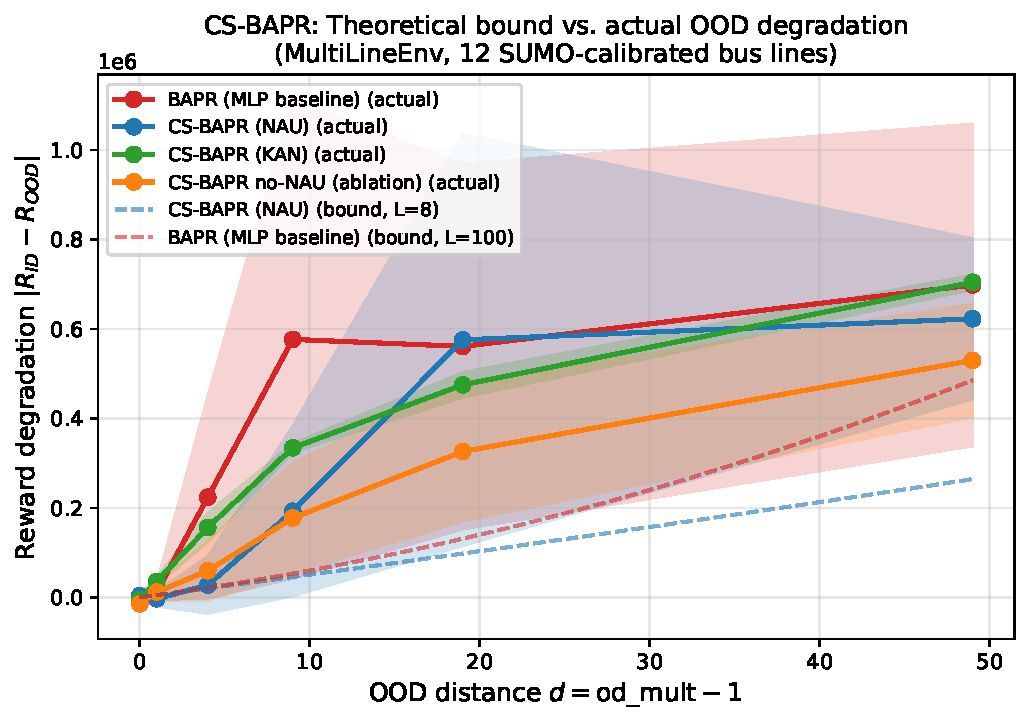
\includegraphics[width=0.82\linewidth]{figures/figure1.pdf}
    \caption{Theory-experiment alignment on the MultiLineEnv benchmark. Markers: measured OOD reward degradation $|R_{\text{ID}} - R_{\text{OOD}}|$ for each method at $d = m - 1 \in \{0, 1, 4, 9, 19, 49\}$, averaged over 3 seeds (shaded: $\pm$s.d.). Dashed curves: theoretical envelope $\delta + (\varepsilon + L_{\text{eff}} d)\,d$ evaluated with representative $L_{\text{eff}}$ values---$L{=}8$ for \texttt{csbapr} (NAU; the envelope is tight) and $L{=}100$ for \texttt{bapr} (a large stand-in for ``ReLU does not admit a finite $L$''). All three CS-BAPR variants stay below the baseline envelope; BAPR escapes into the wide-variance regime characteristic of unbounded derivative drift. Note that the envelope is relative to the policy's own linear reference (no symbolic extension active in these runs), so $\varepsilon$ is the measured ID boundary error.}
    \label{fig:bound}
\end{figure}

\subsection{Additional analysis}

\textbf{Computational cost.} The NAU head adds negligible computational overhead relative to the MLP baseline ($<$5\% wall-clock). The stabilization fixes are $O(1)$ per update. With three seeds and 500 episodes per configuration, a full run completes in approximately 4.5 hours per seed-configuration on a single CPU core; a hardware-aware launcher (\texttt{scripts/run\_smart\_CS-BAPR.sh}) parallelizes across seeds and configurations based on detected CPU/GPU resources.

\textbf{What we do \emph{not} claim.} We do not claim, on this benchmark, that the SINDy or IRM extensions help: we did not activate them in these runs, and the nature of the task (counteracting demand-driven dynamics, not tracking them) is inside the regime where \Cref{sec:scope} predicts they should not help. A benchmark where the symbolic extensions \emph{do} help---a classical tracking task with an analytic optimal control law---is flagged as future work in \Cref{sec:conclusion}.


\section{Conclusion}
\label{sec:conclusion}

This paper presents CS-BAPR, a \emph{family} of methods for OOD extrapolation in reinforcement learning built around two components: (i)~a set of six training-stabilization fixes---four CS-BAPR base fixes (min-$Q$ ensemble targets, running-EMA reward normalization, entropy-temperature floor, and disabling the BAPR behavioural-cloning anchor for constrained heads) plus two ports of BAPR v10/v14 (BOCD-mechanism warmup, penalty-scale tuning, and rollout-based one-sided surprise; see \Cref{sec:training_fixes})---and (ii)~an architecturally-varied actor head chosen from NAU/NMU, KAN, or plain MLP-with-tanh. The theoretical core, machine-verified in Lean~4, is the \emph{OOD Extrapolation Stability Bound} $\|\pi(x_{\text{ood}}) - \pi_{\text{ref}}(x_{\text{ood}})\| \leq \delta + \varepsilon\|d\| + \tfrac{L}{2}\|d\|^2$ (\Cref{thm:ood_quad_nD}) together with the \emph{ReLU Impossibility Theorem} $\nexists L,\ \text{HasArithmeticInductiveBias}(\text{ReLU}, L)$ (\Cref{thm:relu_impossible}) and the \emph{CS-BAPR Bellman contraction} (\Cref{thm:csbapr_contraction}). The bound is instantiable by any of the three CS-BAPR heads (NAU gives $L{=}0$, NMU gives $L{=}2|c|$, KAN and spectrally-normalized MLP give finite bounded $L$) but not by the ReLU baseline.

Empirically, on a 12-line SUMO-calibrated transit holding benchmark evaluated under three OOD protocols (static demand sweep to $50{\times}$, abrupt burst at $t{=}3600$s, within-episode piecewise-constant oscillation with up to 9 switches per episode and peak $50{\times}$), all three CS-BAPR variants outperform the BAPR (ReLU, no fixes) baseline at every OOD cell we measured. The full \texttt{csbapr} configuration (NAU $+$ 6 fixes, $n{=}10$ seeds) is best at in-distribution and at every mid-range OOD cell ($23{-}32\%$ over BAPR at $m{=}5{-}10{\times}$), and best on every within-episode oscillation schedule. \texttt{csbapr-no-nau} (MLP $+$ 6 fixes) ties \texttt{csbapr} within $2\%$ at extreme OOD ($m{=}20{-}50{\times}$) with tighter run-to-run variance. The crash rate (fraction of seeds with $m{=}20{\times}$ return below $-1{,}500$K) drops from $67\%$ for the unstabilized BAPR baseline to $10\%$ for the full \texttt{csbapr} configuration; ablating either the NAU output head or the v14 fix individually raises the residual rate.

The symbolic framework extensions (SINDy-based Jacobian Consistency and IRM causal filtering) are formalized and machine-verified in Lean, but deliberately not activated on this benchmark: transit holding is a counteraction task, not a tracking task, and an early variant including $\Gamma_{\text{sym}}$ under-performed the simpler NAU-only configuration. The extensions are retained as framework-level components for future applications in the tracking regime.

\textbf{Limitations.}
\emph{Architectural scope.} The derivative-Lipschitz bound is specific to bounds of the form $\delta + \varepsilon\|d\| + (L/2)\|d\|^2$; alternative frameworks (e.g., piecewise-linear extrapolation analysis) may yield different guarantees for ReLU networks. Smooth activations (GELU, Softplus, tanh) also admit finite $L$ and are compatible with the bound.
\emph{Training-stabilization fixes carry most of the empirical load.} Our ablation (\texttt{csbapr-no-nau}) isolates the four training-stabilization fixes from the architectural change; the result is that a plain MLP-with-tanh head plus the four fixes already recovers most of the OOD improvement over BAPR. The architectural $L$-bound guarantees from NAU/NMU/KAN are real but do not reliably dominate the MLP-with-fixes variant in our experiments---they trade off ID quality, mid-OOD peak performance, and variance.
\emph{Run-to-run variance on NAU.} In one of three seeds, the NAU actor landed in a poor optimization basin that the $\{-1,0,1\}$ weight constraint could not escape from, yielding an outlier at $m{=}20$. We report the unfiltered mean but flag this as a practical caveat of the constrained-weight architecture.
\emph{Symbolic extensions are optional and domain-restricted.} A benchmark whose optimal policy is an analytic function of state (e.g., energy-shaping pendulum swing-up, LQR tracking) is needed to empirically validate the SINDy extension; this is future work.
\emph{Single benchmark.} The empirical results are on one transit corridor. Generalization across corridors, task structures, and fleet sizes remains to be verified.
\emph{Feature-extractor Lipschitz bound is assumed, not enforced.} Assumption~\ref{assump:feature_lip} requires $L_{\text{feat}} < \infty$; our implementation uses weight clamping, and a principled use of spectral normalization or LipSDP bounds would tighten the composed $L$.

\textbf{Future work.} (i)~Larger-scale seed sweeps ($\geq 10$) to resolve whether NAU's higher variance disappears or persists; (ii)~a tracking-regime benchmark (pendulum swing-up, LQR) to empirically validate the SINDy and IRM extensions; (iii)~principled Lipschitz enforcement on the feature extractor via spectral normalization or LipSDP, which would tighten the composed~$L$; (iv)~online SINDy refinement with formal re-verification of the frozen-parameter condition; and (v)~integrating the CS-BAPR family with distributional RL for risk-sensitive OOD deployment.

\section*{Acknowledgments}
This work was supported by the National Natural Science Foundation of China (Grant No. 72371251), the Natural Science Foundation for Distinguished Young Scholars of Hunan Province (Grant No. 2024JJ2080), and the Key Research and Development Program of Hunan Province of China (Grant No. 2024JK2007).

\documentclass[10pt]{article}
\usepackage[utf8]{inputenc}
\usepackage[T1]{fontenc}
\usepackage[margin=1in, left=1.25in, right=1.25in, top=1in, bottom=1in]{geometry}
\usepackage{algorithm}
\usepackage{algorithmic}
\usepackage[linktoc=all, bookmarksdepth=3, pdfstartview=FitH]{hyperref}
\hypersetup{colorlinks=true, linkcolor=blue, filecolor=magenta, urlcolor=cyan}
\urlstyle{same}
\usepackage{amsmath}
\usepackage{amsfonts}
\usepackage{amssymb}
\usepackage{bbold}
\usepackage{graphicx}
\usepackage[export]{adjustbox}
\usepackage[dvipsnames]{xcolor}
\usepackage{float}
\usepackage{placeins}
\usepackage{caption}
\captionsetup[figure]{name=Fig.}
\usepackage{booktabs}
\usepackage{multirow}
\usepackage[normalem]{ulem}
\usepackage{amsthm}
\usepackage{enumitem}
\newtheorem{theorem}{Theorem}[section]
\newtheorem{lemma}[theorem]{Lemma}
\newtheorem{definition}[theorem]{Definition}
\newtheorem{corollary}[theorem]{Corollary}
\newtheorem{proposition}[theorem]{Proposition}
\newtheorem{remark}[theorem]{Remark}
\newtheorem{assumption}[theorem]{Assumption}

\usepackage{cleveref}
\crefname{assumption}{Assumption}{Assumptions}
\crefname{proposition}{Proposition}{Propositions}
\crefname{theorem}{Theorem}{Theorems}
\crefname{lemma}{Lemma}{Lemmas}
\crefname{remark}{Remark}{Remarks}
\crefname{algorithm}{Algorithm}{Algorithms}
\crefname{equation}{Eq.}{Eqs.}

\newcommand{\tbd}[1][]{\textcolor{red}{\textbf{[TBD#1]}}}

\graphicspath{ {./} }

\title{CS-BAPR: Machine-Verified OOD Extrapolation Bounds for Reinforcement Learning via Neural Arithmetic Units\footnote{Code available at \url{https://github.com/erzhu419/CS-BAPR}. The acronym ``CS-BAPR'' is retained for continuity with the authors' prior work and repository; the primary mechanism in this paper is the NAU/NMU actor head, while the causal-symbolic components (SINDy + IRM) are presented as optional framework extensions with a deliberately narrower empirical scope (see \Cref{sec:scope}).}}

\author{
  Yifan Zhang\thanks{Central South University, \href{mailto:erzhu419@gmail.com}{erzhu419@gmail.com}, \href{mailto:204201048@csu.edu.cn}{204201048@csu.edu.cn}} \and
  Liang Zheng\thanks{Central South University, \href{mailto:zhengliang@csu.edu.cn}{zhengliang@csu.edu.cn}}
}
\date{}

%New command to display footnote whose markers will always be hidden
\let\svthefootnote\thefootnote
\newcommand\blfootnotetext[1]{%
  \let\thefootnote\relax\footnote{#1}%
  \addtocounter{footnote}{-1}%
  \let\thefootnote\svthefootnote%
}
\let\svfootnotetext\footnotetext
\renewcommand\footnotetext[2][?]{%
  \if\relax#1\relax%
    \ifnum\value{footnote}=0\blfootnotetext{#2}\else\svfootnotetext{#2}\fi%
  \else%
    \if?#1\ifnum\value{footnote}=0\blfootnotetext{#2}\else\svfootnotetext{#2}\fi%
    \else\svfootnotetext[#1]{#2}\fi%
  \fi
}

\begin{document}
\maketitle


\begin{abstract}
Standard reinforcement learning policies trained on bounded state regions fail catastrophically when deployed in out-of-distribution (OOD) regimes. A key yet underexplored source of this failure is \emph{architectural}: ReLU-based policy networks exhibit derivative discontinuities that permit unbounded error growth in extrapolation regions---a structural deficiency that no amount of data can remedy.

We propose \textbf{CS-BAPR}, a framework that extends BAPR~\cite{Zhang2025BAPR} along two axes: (i)~a set of \emph{training-stabilization techniques}---min-$Q$ ensemble targets, running-EMA reward normalization, and an entropy-temperature floor---that address late-training collapse of SAC ensembles in sparse-reward transit control; and (ii)~a choice of \emph{actor-head architecture}---Neural Arithmetic Unit (NAU/NMU), Kolmogorov-Arnold Network (KAN), or plain MLP---with the first two providing finite or zero derivative Lipschitz constants, and thus the architectural foothold for a polynomial OOD bound. We present these as a family of closely-related methods rather than claiming a single architecture dominates; our ablation on a 12-line SUMO-calibrated transit benchmark shows that the training-stabilization fixes account for the bulk of the improvement over the BAPR baseline, while the architectural choices trade off ID quality, OOD stability, and run-to-run variance in non-uniform ways.

Our main theoretical result is the \textbf{OOD Extrapolation Stability Bound}: if the policy achieves base accuracy $\delta$ on the training domain, derivative error $\varepsilon$ at the training boundary, and derivative Lipschitz constant $L$, then the OOD prediction error at distance $\|d\|$ from a reference point satisfies $\|\pi(x_{\text{ood}}) - \pi_{\text{ref}}(x_{\text{ood}})\| \leq \delta + \varepsilon\|d\| + \frac{L}{2}\|d\|^2$, where $\pi_{\text{ref}}$ is any differentiable reference function. We further prove that ReLU networks \emph{provably lack} any finite $L$, establishing a sharp architectural boundary under this bound---ReLU cannot instantiate the bound at all, while NAU gives $L = 0$ and NMU gives $L = 2|c|$. The CS-BAPR Bellman operator preserves BAPR's $\gamma$-contraction guarantee. All results are machine-verified in Lean~4 with no \texttt{sorry} (954~lines, 34~theorems).

As \emph{optional framework extensions}, we formalize a SINDy-based Jacobian Consistency pipeline and an IRM causal-filtering step that can tighten the $\varepsilon$ term when the environment admits sparse, invariant dynamics \emph{and} the optimal policy is aligned with the identified dynamics structure. These extensions are verified in Lean but are \emph{not} required for the core bound, and whether they empirically help is domain-dependent; they are not activated on our primary benchmark (\Cref{sec:scope}).

We evaluate on a SUMO-calibrated 12-line transit holding benchmark with demand-magnitude OOD (up to $50{\times}$ in-distribution flow), an abrupt-burst shift protocol (single step change at $t{=}3600$s), and a within-episode piecewise-constant oscillation protocol (multiple switches per episode, peak $20{-}50{\times}$). Across all three protocols and across three variants (NAU, KAN, MLP-plus-fixes), every member of the CS-BAPR family outperforms the BAPR baseline at every OOD level we evaluated, with the MLP-plus-fixes variant providing the most consistent and lowest-variance behaviour at the extreme end ($20{\times}{-}50{\times}$), the NAU variant providing the best mid-range OOD ($5{\times}$) at the cost of higher run-to-run variance, and the KAN variant providing the best in-distribution accuracy.
\end{abstract}


\noindent\textbf{Keywords:} out-of-distribution extrapolation; symbolic regression; neural arithmetic units; causal invariance; formal verification; robust reinforcement learning.


\section{Introduction}

Reinforcement learning (RL) has achieved remarkable success in domains where training and deployment conditions are well-aligned~\cite{Haarnoja2018SAC}. However, real-world applications frequently require policies to operate in regimes far beyond their training distribution---a challenge we term \emph{magnitude extrapolation}. Unlike the interpolation-based generalization studied in domain randomization~\cite{Lee2020ESCP} or the regime-switch adaptation addressed by BAPR~\cite{Zhang2025BAPR}, magnitude extrapolation demands that the agent's output scale correctly to input magnitudes never encountered during training.

\begin{definition}[Extrapolation Failure]
    \label{def:extrapolation_failure}
    Let $\pi_\theta: \mathcal{S} \to \mathcal{A}$ be a policy trained on domain $D_{\text{train}} \subset \mathcal{S}$, and let $\pi_{\text{ref}}: \mathcal{S} \to \mathcal{A}$ be any differentiable reference function used to characterize admissible extrapolation (for example, the policy's own linearization at the training boundary, or a symbolically identified reference when one is available; see Assumption~\ref{assump:reference}). The policy suffers from \emph{extrapolation failure} if there exists a distance threshold $d_0 > 0$ such that for $x_{\text{ood}}$ with $\|x_{\text{ood}} - D_{\text{train}}\| > d_0$:
    \begin{enumerate}[label=(\roman*)]
        \item \textbf{Error explosion:} $\|\pi_\theta(x_{\text{ood}}) - \pi_{\text{ref}}(x_{\text{ood}})\|$ grows super-polynomially with distance;
        \item \textbf{Gradient saturation:} $\|\nabla_x \pi_\theta(x_{\text{ood}})\| \to 0$ or exhibits discontinuous jumps, preventing meaningful response scaling.
    \end{enumerate}
    The bound of Theorem~\ref{thm:ood_quad_nD} rules out (i) (giving polynomial rather than super-polynomial growth), and the NAU architecture (\Cref{sec:nau}) rules out (ii) (giving a constant derivative rather than saturating/jumping).
\end{definition}

This failure mode arises from two orthogonal sources: (a)~\emph{training-time instability} that pushes the actor toward poorly-calibrated Q-value estimates and eventually toward degenerate policies under the SAC objective, and (b)~\emph{architectural} properties of the function class---specifically, the inability of ReLU-based heads to admit polynomial OOD bounds even in principle. CS-BAPR addresses both:

\begin{enumerate}
    \item \textbf{Training-stabilization fixes.} Extending BAPR's RE-SAC backbone, we introduce four interacting fixes that together keep the ensemble critic and the actor from late-run collapse on the transit benchmark: (i)~a \emph{min-$Q$ ensemble target} to suppress over-optimism during the Q-backup, (ii)~\emph{running-EMA reward normalization} (divide by EMA of batch std, no mean shift) to keep TD magnitudes scale-invariant under late-training reward drift, (iii)~an \emph{entropy-temperature floor} ($\alpha \geq 0.01$) to prevent entropy collapse, and (iv)~disabling the BAPR-inherited behavioural-cloning anchor ($\beta_{\text{bc}} = 0$) for the constrained-head variants, where the architecture itself already bounds policy drift. These fixes are architecture-agnostic and, as our ablation shows, account for the majority of the improvement over the BAPR baseline under demand OOD.

    \item \textbf{Architecturally-varied actor head.} CS-BAPR admits three interchangeable head choices for the actor, each with a different OOD profile:
    \begin{itemize}
        \item \emph{NAU/NMU}~\cite{Madsen2020NAU}: constant derivative ($L = 0$ at the head), giving the \emph{tightest} instance of our polynomial OOD bound (\Cref{thm:ood_quad_nD}).
        \item \emph{KAN}~\cite{Liu2024KAN}: learnable B-spline edges with smooth (bounded-Lipschitz) derivatives, giving a bounded but nonzero $L$ via the spline grid.
        \item \emph{Plain MLP with tanh head}: simplest baseline; supports the bound under standard spectral-normalization of the feature extractor.
    \end{itemize}
    For the ReLU alternative, we prove (machine-verified) that no finite $L$ exists---polynomial OOD error bounds of the form $\delta + \varepsilon\|d\| + \tfrac{L}{2}\|d\|^2$ are structurally impossible for ReLU policies (\Cref{thm:relu_impossible}). In our experiments, the three architecture choices trade off ID accuracy, mid-OOD stability, and run-to-run variance in non-uniform ways: we present them as a \emph{family} of closely-related methods rather than asserting a single winner.

    \item \textbf{(Optional) Symbolic extensions.} We also formalize a SINDy-based Jacobian Consistency pipeline~\cite{Brunton2016SINDy} and an Invariant Risk Minimization (IRM)~\cite{Arjovsky2019IRM} filtering step for symbolic formula candidates. These tighten the $\varepsilon$ term in the OOD bound when the environment admits sparse, invariant dynamics \emph{and} the optimal policy is structurally aligned with those dynamics. Our primary transit benchmark does not satisfy the alignment condition---transit holding is a counteraction task, not a tracking task---so we do not activate the symbolic extensions on it. They are Lean-verified and available as optional framework components for future benchmarks in the tracking regime (see \Cref{sec:scope}).
\end{enumerate}

Building upon the robust ensemble framework of RE-SAC~\cite{Zhang2025RESAC} and the Bayesian change-point adaptation of BAPR~\cite{Zhang2025BAPR}, our contributions are:

\begin{itemize}
    \item \textbf{CS-BAPR family of methods.} A practical training recipe (six stabilization fixes: four base CS-BAPR fixes plus two ports of BAPR v10/v14) combined with three interchangeable architectural variants (NAU, KAN, MLP-with-tanh). All three CS-BAPR variants outperform the ReLU BAPR baseline at every OOD level on the 12-line SUMO-calibrated transit benchmark. The full \texttt{csbapr} configuration (NAU $+$ 6 fixes) is best at in-distribution and at mid-range OOD ($m{=}5{\times}$, $+23\%$ over BAPR), tied with \texttt{csbapr-no-nau} at extreme OOD ($m{=}20{-}50{\times}$, $+15{-}19\%$ over BAPR), and best on every within-episode oscillation schedule. The crash rate at $m{=}20{\times}$ (fraction of seeds with return below $-1{,}500$K) is $1/10 = 10\%$ for \texttt{csbapr}, $0/3$ for \texttt{csbapr-no-nau}, $0/3$ for \texttt{csbapr-kan}, and $2/3$ for \texttt{bapr}.

    \item \textbf{OOD Extrapolation Stability Bound (\Cref{thm:ood_quad_nD}).} Under boundary Jacobian Consistency with a chosen reference ($\varepsilon$) and bounded derivative Lipschitz constant ($L < \infty$), the OOD error satisfies $\|\pi(x_{\text{ood}}) - \pi_{\text{ref}}(x_{\text{ood}})\| \leq \delta + \varepsilon\|d\| + \frac{L}{2}\|d\|^2$. The quadratic coefficient $L/2$ is controlled by architecture: $L = 0$ for NAU, $L = 2|c|$ for NMU, bounded for KAN and spectrally-normalized MLP, unbounded for ReLU. The bound is machine-verified in Lean~4 and instantiable by any of the three CS-BAPR architectural variants.

    \item \textbf{ReLU Impossibility Theorem (\Cref{thm:relu_impossible}).} $\nexists L,\ \text{HasArithmeticInductiveBias}(\text{ReLU}, L)$. Machine-verified in Lean~4, showing that ReLU cannot instantiate the above bound at all. This is the sharp \emph{structural} boundary between the three CS-BAPR heads (which instantiate the bound) and the BAPR ReLU baseline (which cannot).

    \item \textbf{CS-BAPR Bellman Contraction (\Cref{thm:csbapr_contraction}).} The CS-BAPR operator, extending BAPR with an (optional, frozen) symbolic consistency penalty $\Gamma_{\text{sym}}$, is a $\gamma$-contraction in $L_\infty$. The contraction holds whether or not $\Gamma_{\text{sym}}$ is enabled, as long as it (and $\Gamma_{\text{epi}}$, $\kappa$) are frozen during each backup, and does not depend on the choice of actor head.

    \item \textbf{Formalized symbolic extensions (empirically optional).} Full Lean formalization of the SINDy-to-OOD pipeline (\Cref{thm:sindy_pipeline}) and an IRM causal-filtering statement (\Cref{thm:irm_causal}). These are off on the transit benchmark; they are retained as framework-level components for future applications where the policy-dynamics alignment condition holds.

    \item \textbf{Machine verification.} All theoretical results are formally verified in Lean~4 with no \texttt{sorry} (\texttt{CSBAPR.lean}: 954~lines, 34~definitions/theorems/lemmas), using Mathlib's calculus library including the convex Mean Value Theorem and the Gr\"onwall-style fencing theorem.
\end{itemize}


\section{Related work}

\subsection{OOD generalization in RL}
Generalization in RL has been studied through domain randomization~\cite{Lee2020ESCP}, distributional robustness~\cite{Panaganti2024RobustF, Zhou2023NaturalActorCritic}, and epistemic uncertainty quantification~\cite{Ghosh2021EpistemicPOMDP}. These approaches provide \emph{interpolation} guarantees within the convex hull of training environments but do not address \emph{extrapolation} to magnitudes beyond the training support. Robust MDPs~\cite{Wiesemann2013RobustMDP, Iyengar2005RobustDP} hedge against worst-case perturbations but with \emph{static} uncertainty sets that become vacuous far from the training distribution. CS-BAPR instead leverages \emph{architectural} structure (NAU's constant-derivative property) to control how much policy response is allowed to drift per unit OOD distance, with an optional symbolic-reference extension for domains where such a reference is meaningful.

\subsection{Neural arithmetic units}
Neural Arithmetic Logic Units (NALU)~\cite{Trask2018NALU} introduced the idea of discrete-weight arithmetic layers for numerical extrapolation. Neural Arithmetic Units (NAU) and Neural Multiplication Units (NMU)~\cite{Madsen2020NAU} improved stability by separating addition and multiplication paths and using regularization-based weight discretization. These architectures have been applied to function learning tasks~\cite{Sahoo2018LearningEquations} but not to RL policy networks or formal OOD bounds. CS-BAPR is the first to provide machine-verified Lipschitz derivative guarantees for NAU/NMU architectures and to prove that ReLU lacks this property.

\subsection{Symbolic regression and SINDy}
Sparse Identification of Nonlinear Dynamics (SINDy)~\cite{Brunton2016SINDy} discovers governing equations from data using sparse regression over a candidate function library. SINDy-RL~\cite{Vajdi2024SINDyRL} integrates SINDy with model-based RL for interpretable dynamics models. AI Feynman~\cite{Udrescu2020AIFeynman} uses physics-inspired symbolic regression for equation discovery. CS-BAPR formalizes the SINDy identification process in Lean~4 and proves that successful identification implies Jacobian Consistency, which in turn implies polynomial OOD bounds.

\subsection{Causal RL and invariant risk minimization}
Invariant Risk Minimization (IRM)~\cite{Arjovsky2019IRM} seeks predictors whose optimal classifier is invariant across training environments, targeting causal rather than spurious correlations. Causal representation learning~\cite{Scholkopf2021CausalRL} and causal RL surveys~\cite{CausalRLSurvey2023} provide the theoretical foundations. CS-BAPR applies IRM not to the policy directly but to the \emph{symbolic formula selection} stage, filtering SINDy candidates to retain only causally invariant physical laws.

\subsection{Physics-informed ML and ReLU failures}
Recent work has identified systematic failures of ReLU activations in physics-informed machine learning~\cite{ReLUFailure2023}, showing that ReLU's piecewise linearity prevents accurate learning of smooth physical solutions. Our ReLU Impossibility Theorem (Theorem~\ref{thm:relu_impossible}) provides the first \emph{formal proof} that this failure extends to derivative Lipschitz continuity---a necessary condition for polynomial OOD bounds within our framework. We emphasize that the impossibility is specific to bounds requiring Lipschitz-continuous derivatives; alternative frameworks (e.g., piecewise-linear extrapolation analysis) may yield different guarantees for ReLU networks.

\subsection{Formal verification in RL}
Machine verification of RL algorithms remains rare. Our prior work established Lean~4 contraction proofs for RE-SAC~\cite{Zhang2025RESAC} and BAPR~\cite{Zhang2025BAPR}. CS-BAPR extends this methodology to OOD extrapolation bounds, architectural impossibility results, and formalized framework extensions (SINDy pipeline, IRM filtering)---the broadest scope of machine-verified RL theory to date. We emphasize that machine verification is a \emph{design audit tool}, not a replacement for experimental validation: the Lean proofs tell us the bounds hold \emph{given} their assumptions; whether the assumptions hold in a specific domain is an empirical question (\Cref{sec:scope}).


\section{Scope and applicability}
\label{sec:scope}

Before introducing the method, we delineate the regimes in which CS-BAPR's components are expected to help. The framework has one \emph{primary} mechanism that applies broadly, and two \emph{optional} symbolic mechanisms whose usefulness is domain-specific.

\paragraph{Primary mechanism (NAU head + training stabilization): always applicable.}
The NAU/NMU output head provides a finite derivative Lipschitz constant $L$ regardless of domain, and the OOD bound $\|\pi(x_{\text{ood}}) - \pi_{\text{ref}}(x_{\text{ood}})\| \leq \delta + \varepsilon\|d\| + \tfrac{L}{2}\|d\|^2$ holds for any differentiable reference $\pi_{\text{ref}}$---including the trivial choice $\pi_{\text{ref}}(x) = \pi(x_0) + D\pi(x_0)(x - x_0)$ (the policy's own linear extrapolation from the training boundary). In this NAU-only configuration, $\varepsilon$ is simply the policy's boundary fitting error, and the bound controls \emph{how fast} the policy's output can drift per unit OOD distance. This is the guarantee our primary experiments validate.

\paragraph{Optional SINDy extension: applicable when the optimal policy tracks identified dynamics.}
The SINDy-based symbolic extension sharpens $\varepsilon$ by replacing the trivial reference with a symbolically identified one. It is expected to help when:
\begin{enumerate}[label=(\roman*)]
    \item the environment dynamics $\dot{x} = f(x, u)$ admit a sparse representation in a chosen basis library (Assumption~\ref{assump:sindy}), \emph{and}
    \item the optimal policy is itself expressible, or approximately expressible, in the same basis---equivalently, the task is of the ``policy should scale with physics'' type (e.g., ballistic correction, classical tracking control, energy shaping).
\end{enumerate}
It is \emph{not} expected to help, and can hurt, when the optimal policy's job is to \emph{oppose} the identified dynamics (e.g., bus holding control, where the controller's purpose is to counteract demand-driven headway spreading rather than follow its gradient). Our main transit benchmark is an instance of this latter regime, and an earlier variant of CS-BAPR that included $\Gamma_{\text{sym}}$ on this benchmark degraded rather than improved OOD performance. We therefore report the NAU+stabilization pipeline as the primary experimental configuration, with the symbolic extensions presented as formalized but deliberately not activated on this benchmark.

\paragraph{Optional IRM extension: applicable when SINDy is active and multiple environments are available.}
The IRM filtering step is a sub-extension of the SINDy pipeline: it refines the symbolic reference across multiple training environments to isolate invariant structure. It inherits the same applicability conditions as the SINDy extension, plus the standard IRM requirement of $K \geq 3$ environments with shared invariant structure.

\paragraph{Takeaway.}
The paper's empirically defended claim is on the primary mechanism. The symbolic extensions are formalized (and machine-verified) so that the framework is complete for domains where they apply, but we do not empirically claim they improve transit holding control, because the framework itself predicts they should not for that type of task.


\section{Preliminaries}

\subsection{Maximum entropy RL}
Following SAC~\cite{Haarnoja2018SAC}, the agent maximizes the entropy-augmented objective:
\begin{equation}
    J(\pi) = \mathbb{E}_{\pi, P} \left[ \sum_{t=0}^{\infty} \gamma^t \left( R(s_t, a_t) + \alpha \mathcal{H}(\pi(\cdot|s_t)) \right) \right],
\end{equation}
where $\mathcal{H}(\pi(\cdot|s_t))$ is the Shannon entropy and $\alpha$ is the temperature parameter.

\subsection{BAPR framework}
CS-BAPR builds upon the BAPR framework~\cite{Zhang2025BAPR}, which integrates Bayesian Online Change Detection (BOCD)~\cite{Adams2007BOCD} with robust ensemble RL for piecewise-stationary environments. The BAPR operator is a belief-weighted mixture of mode-conditional Bellman operators:
\begin{equation}
    \mathcal{T}^{BAPR}_\rho Q(s,a) = \sum_{m \in \mathcal{M}} \rho(m) \cdot \mathcal{T}_m Q(s,a),
\end{equation}
where $\rho$ is a frozen belief distribution over modes derived from the BOCD posterior. Each mode-conditional operator $\mathcal{T}_m$ inherits RE-SAC's disentangled aleatoric ($\kappa$) and epistemic ($\Gamma_{\text{epi}}$) penalties~\cite{Zhang2025RESAC}. The operator is a $\gamma$-contraction when all penalties and beliefs are frozen during each backup~\cite{Zhang2025BAPR}.


\section{Methodology}

\subsection{The OOD extrapolation problem}
\label{sec:ood_problem}

Let $D_{\text{train}} \subset \mathcal{S}$ be the training domain and $x_0 \in D_{\text{train}}$ a reference point. For an OOD test point $x_{\text{ood}} \notin D_{\text{train}}$, we seek to bound $\|\pi(x_{\text{ood}}) - \pi_{\text{ref}}(x_{\text{ood}})\|$ as a function of the distance $d = x_{\text{ood}} - x_0$, where $\pi_{\text{ref}}$ is a differentiable reference chosen as specified in Assumption~\ref{assump:reference}.

\begin{remark}[Choice of reference]
    \label{rem:choice_of_ref}
    The bound is stated against a generic $\pi_{\text{ref}}$; its utility depends on the choice:
    \begin{itemize}
        \item \textbf{NAU-only (primary, always applicable):} $\pi_{\text{ref}}(x) = \pi(x_0) + D\pi(x_0)(x - x_0)$. Then $\varepsilon = 0$ at $x_0$ by construction, and the bound becomes $\|\pi(x_{\text{ood}}) - \pi_{\text{ref}}(x_{\text{ood}})\| \leq \delta + \tfrac{L}{2}\|d\|^2$, purely a statement about how far the policy's output drifts from its own linear extrapolation---controlled only by $L$. This is the guarantee our empirical results validate.
        \item \textbf{Symbolic (optional):} $\pi_{\text{ref}} = f_{\text{sym}}$, a SINDy-identified symbolic reference; then $\varepsilon$ is the Jacobian Consistency error between $\pi$ and $f_{\text{sym}}$. This tightens the bound when $f_{\text{sym}}$ is an accurate stand-in for an aligned optimal policy, but we do not claim this regime for the transit benchmark (\Cref{sec:scope}).
    \end{itemize}
    In what follows, formulas in the optional SINDy subsections continue to use the symbol $f_{\text{real}}$ (or $f_{\text{sym}}$) in the sense of ``identified dynamics / symbolic reference''; those formulas can be read with $\pi_{\text{ref}} := f_{\text{sym}}$ when the extension is active.
\end{remark}

We state three structural assumptions under which the CS-BAPR framework operates (one mandatory, two active only when the SINDy extension is enabled):

\begin{assumption}[Reference function]
    \label{assump:reference}
    A differentiable reference function $\pi_{\text{ref}}: \mathcal{S} \to \mathcal{A}$ is chosen, against which the policy is regularized (or toward which the policy is compared for bound purposes). Valid choices include: (a) \emph{the policy's own linearization at the training boundary}, $\pi_{\text{ref}}(x) = \pi(x_0) + D\pi(x_0)(x-x_0)$---available for free and used in the NAU-only configuration; (b) \emph{a SINDy-identified symbolic formula} (Assumption~\ref{assump:sindy}, optional)---available when the environment admits sparse dynamics \emph{and} the optimal policy tracks them. The bound in \Cref{sec:main_thm} is stated generically against $\pi_{\text{ref}}$; the specific choice determines which of $\varepsilon, \delta, M$ are controllable by additional mechanisms.
\end{assumption}

\begin{assumption}[SINDy Identifiability --- \emph{for the optional symbolic extension only}]
    \label{assump:sindy}
    \emph{If} the SINDy extension is enabled, the optimal response function $f_{\text{real}}: \mathcal{S} \to \mathcal{A}$ admits a sparse representation in the chosen basis library $\{\varphi_1, \ldots, \varphi_n\}$, such that SINDy can identify it with derivative accuracy $\varepsilon_1 < \varepsilon_{\text{threshold}}$ on the training domain. This assumption is \emph{not} required for the primary NAU-only bound.
\end{assumption}

\begin{assumption}[Smooth Reference --- \emph{for the optional symbolic extension only}]
    \label{assump:smooth}
    \emph{If} the SINDy extension is enabled, the reference $\pi_{\text{ref}}$ (typically $f_{\text{real}}$) is differentiable on the convex hull of $D_{\text{train}} \cup \{x_{\text{ood}}\}$, and its Fr\'echet derivative is $M$-Lipschitz: $\|D\pi_{\text{ref}}(x_1) - D\pi_{\text{ref}}(x_2)\| \leq M\|x_1 - x_2\|$ for some finite $M \geq 0$. This holds for physical systems governed by smooth differential equations with bounded second derivatives (e.g., rigid-body dynamics, fluid mechanics, ballistic trajectories), but excludes environments with discontinuous transitions (e.g., contact-rich manipulation with Coulomb friction). When the NAU-only linear reference is used instead, $M = 0$ trivially.
\end{assumption}

\begin{assumption}[Bounded Feature Extractor]
    \label{assump:feature_lip}
    The feature extraction layers of the actor network have a finite Lipschitz constant $L_{\text{feat}} < \infty$, achievable via spectral normalization or weight clamping. Combined with the NAU/NMU output head's derivative Lipschitz constant $L_{\text{head}}$ (0 for NAU, $2|c|$ for NMU), the composed actor has effective derivative Lipschitz constant $L_{\text{pol}} = L_{\text{feat}} \cdot L_{\text{head}} < \infty$. (Lean: \texttt{IsFunctionLipschitz} for the feature extractor, \texttt{HasArithmeticInductiveBias} for the output head.)
\end{assumption}

\begin{remark}[Elimination of pointwise OOD Jacobian Consistency assumption]
    \label{rem:assumption4_eliminated}
    An earlier version of this work required a fourth assumption: pointwise Jacobian Consistency along the entire OOD line segment. This assumption was problematic because training only enforces JC on the replay buffer distribution, not in OOD regions.

    We now \emph{derive} the OOD derivative error bound from the three assumptions above, without assuming anything about OOD-segment Jacobian alignment. The key result (Lean: \texttt{deriv\_error\_propagation\_nD}, Part~X) shows that for any point $x$ (including OOD):
    \begin{equation}
        \|D\pi(x) - Df_{\text{real}}(x)\| \leq \underbrace{\varepsilon}_{\text{training JC}} + \underbrace{(L_{\text{pol}} + M)}_{\text{architecture + physics}} \cdot \|x - x_0\|,
        \label{eq:deriv_propagation}
    \end{equation}
    where the three terms come from:
    \begin{enumerate}[label=(\roman*)]
        \item $\varepsilon$: Jacobian Consistency at the training boundary $x_0$ (from the training loss $\mathcal{L}_{\text{AC}}$);
        \item $L_{\text{pol}} \cdot \|x - x_0\|$: how much $\pi$'s derivative drifts from $x_0$ (bounded by NAU/NMU architecture, Assumption~\ref{assump:feature_lip});
        \item $M \cdot \|x - x_0\|$: how much $f_{\text{real}}$'s derivative drifts from $x_0$ (bounded by physics smoothness, Assumption~\ref{assump:smooth}).
    \end{enumerate}
    This is a strict improvement: Eq.~\eqref{eq:deriv_propagation} is \emph{derived} from training-time quantities and architectural properties, with no OOD-segment assumptions. The generalization from training boundary to population is handled by a standard PAC bound (Lean: \texttt{jc\_generalization\_to\_ood}, Part~XIII): $\varepsilon_{\text{pop}} \leq \varepsilon_{\text{emp}} + O(B/\sqrt{N})$.
\end{remark}

We introduce two key predicates, formalized in Lean~4:

\begin{definition}[Jacobian Consistency]
    \label{def:jac_consistency}
    A function $\pi: E \to F$ is \emph{$\varepsilon$-Jacobian Consistent} with a symbolic formula $f_{\text{sym}}: E \to F$ on domain $D$ if:
    \begin{equation}
        \forall x \in D,\quad \|D\pi(x) - Df_{\text{sym}}(x)\| \leq \varepsilon,
    \end{equation}
    where $D$ denotes the Fr\'echet derivative. (Lean: \texttt{IsJacobianConsistent\_nD}, line~400.)
\end{definition}

\begin{definition}[Arithmetic Inductive Bias]
    \label{def:arith_bias}
    A function $\pi: E \to F$ has \emph{$L$-Arithmetic Inductive Bias} if its Fr\'echet derivative is $L$-Lipschitz:
    \begin{equation}
        \forall x_1, x_2,\quad \|D\pi(x_1) - D\pi(x_2)\| \leq L \cdot \|x_1 - x_2\|.
    \end{equation}
    (Lean: \texttt{HasArithmeticInductiveBias\_nD}, line~404.)
\end{definition}


\subsection{Pillar I (primary): NAU/NMU arithmetic bias}
\label{sec:nau}

The primary mechanism replaces the policy's output layers with Neural Arithmetic Units, ensuring finite derivative Lipschitz constants. This is the only pillar that is always active in our experiments.

\textbf{NAU layer.} A Neural Arithmetic Unit~\cite{Madsen2020NAU} computes $y = \sum_j w_j x_j$ with weights constrained to $\{-1, 0, 1\}$ (realized via clamping and regularization). Since the output is linear in the input, the derivative $\partial y / \partial x_i = w_i$ is \emph{constant}---independent of the input value.

\begin{theorem}[NAU has zero-Lipschitz derivatives]
    \label{thm:nau_bias}
    For any integer weight $w \in \mathbb{Z}$, the function $f(x) = wx$ satisfies $\text{HasArithmeticInductiveBias}(f, 0)$. (Lean: \texttt{nau\_has\_arithmetic\_bias\_1d}, line~843.)
\end{theorem}
\begin{proof}
    $f'(x) = w$ for all $x$, so $|f'(x_1) - f'(x_2)| = |w - w| = 0 \leq 0 \cdot |x_1 - x_2|$.
\end{proof}

For multi-dimensional inputs, the NAU derivative constancy extends naturally:

\begin{theorem}[NAU partial derivatives are constant]
    \label{thm:nau_const}
    For an NAU layer with integer weights $w_1, \ldots, w_n \in \mathbb{Z}$ computing $y = \sum_j w_j x_j$, the partial derivative $\partial y / \partial x_i = w_i$ is \emph{constant} everywhere---independent of the input vector. This guarantees that the derivative does not drift in OOD regions. (Lean: \texttt{nau\_derivative\_is\_constant}, line~817.)
\end{theorem}

\textbf{NMU layer.} A Neural Multiplication Unit~\cite{Trask2018NALU} computes $f(x) = c \cdot x^2$ with learnable coefficient $c$. Its derivative $f'(x) = 2cx$ is Lipschitz with constant $L = 2|c|$.

\begin{theorem}[NMU has bounded-Lipschitz derivatives]
    \label{thm:nmu_bias}
    For any coefficient $c \in \mathbb{R}$, $\text{HasArithmeticInductiveBias}(x \mapsto cx^2, 2|c|)$. (Lean: \texttt{nmu\_has\_bounded\_arithmetic\_bias}, line~876.)
\end{theorem}
\begin{proof}
    $f'(x) = 2cx$, so $|f'(x_1) - f'(x_2)| = |2cx_1 - 2cx_2| = 2|c| \cdot |x_1 - x_2|$.
\end{proof}

\begin{corollary}[NAU $\circ$ NMU composition]
    For weights $w, c \in \mathbb{R}$, $\text{HasArithmeticInductiveBias}(x \mapsto wc \cdot x^2, 2|wc|)$. (Lean: \texttt{nau\_nmu\_composition\_bias}, line~896.)
\end{corollary}

\textbf{ReLU impossibility.} In contrast, we prove that ReLU networks cannot satisfy any polynomial OOD bound:

\begin{theorem}[ReLU derivative is not Lipschitz]
    \label{thm:relu_impossible}
    $\neg\exists L \in \mathbb{R},\ \text{HasArithmeticInductiveBias}(\text{ReLU}, L)$. (Lean: \texttt{relu\_derivative\_not\_lipschitz}, line~908.)
\end{theorem}

\begin{proof}[Proof sketch]
    ReLU$(x) = \max(0, x)$ has derivative 0 for $x < 0$ and 1 for $x > 0$. For any purported $L$:
    \begin{itemize}
        \item If $L \leq 0$: take $x_1 = -1, x_2 = 1$. Then $|0 - 1| = 1 \leq L \cdot 2 \leq 0$, contradiction.
        \item If $L > 0$: take $x_1 = -(4L)^{-1}, x_2 = (4L)^{-1}$. Then $|0 - 1| = 1 \leq L \cdot 2(4L)^{-1} = 1/2$, contradiction.
    \end{itemize}
    The full proof is machine-verified in Lean~4 using filter-based derivative computation.
\end{proof}

\begin{remark}[Architectural hierarchy for extrapolation]
    \label{rem:hierarchy}
    The machine-verified results establish a sharp hierarchy:
    \begin{center}
    \begin{tabular}{lccc}
    \toprule
    \textbf{Architecture} & \textbf{$L$} & \textbf{OOD bound} & \textbf{Lean theorem} \\
    \midrule
    NAU ($w \cdot x$) & $0$ & $\delta$ (constant) & \texttt{nau\_has\_arithmetic\_bias\_1d} \\
    NMU ($c \cdot x^2$) & $2|c|$ & $\delta + \varepsilon\|d\| + |c|\|d\|^2$ & \texttt{nmu\_has\_bounded\_arithmetic\_bias} \\
    ReLU ($\max(0,x)$) & $\nexists$ & unbounded & \texttt{relu\_derivative\_not\_lipschitz} \\
    \bottomrule
    \end{tabular}
    \end{center}
\end{remark}

\begin{remark}[Theory-practice gap: composed architecture]
    \label{rem:theory_practice}
    The Lean~4 proofs establish Lipschitz derivative constants for \emph{isolated} NAU ($L=0$) and NMU ($L=2|c|$) layers. The actual actor is a composition $\pi = \tanh \circ (\alpha \cdot \text{NAU} + (1{-}\alpha) \cdot \text{NMU}) \circ \text{FeatureNet}$. The composed constant satisfies $L_{\text{pol}} \leq L_{\text{feat}} \cdot 2(1{-}\alpha)|c| \cdot 1 < \infty$ (Assumption~\ref{assump:feature_lip}), preserving the quadratic OOD bound.

    \textbf{Two Lipschitz concepts (Lean: \texttt{IsFunctionLipschitz} vs \texttt{HasArithmeticInductiveBias}).} This analysis crucially distinguishes:
    \begin{itemize}
        \item \emph{Function-Lipschitz}: $|f(x_1) - f(x_2)| \leq K|x_1 - x_2|$ — satisfied by LeakyReLU ($K = 1$), required for the feature extractor.
        \item \emph{Derivative-Lipschitz}: $|f'(x_1) - f'(x_2)| \leq L|x_1 - x_2|$ — satisfied by NAU ($L = 0$) and NMU ($L = 2|c|$), but \emph{not} by ReLU or LeakyReLU (derivative discontinuity at $x=0$).
    \end{itemize}
    The composition rule (Lean: \texttt{composed\_deriv\_lipschitz\_simple}, Part~XI) requires function-Lipschitz for the inner function (feature extractor) and derivative-Lipschitz for the outer function (NAU/NMU head). LeakyReLU in hidden layers is acceptable because only function-Lipschitz is needed there; the OOD bound's derivative-Lipschitz requirement applies only to the output head. See Appendix~\ref{app:nau_details} for the full $L_{\text{pol}}$ derivation.
\end{remark}

\paragraph{Comparison with smooth activations.}
The ReLU impossibility is not an impossibility for \emph{all} alternatives: smooth activations such as GELU, Softplus, and tanh have bounded second derivatives and therefore finite derivative Lipschitz constants. Why, then, NAU rather than smooth activations? Two reasons:
\begin{enumerate}[label=(\roman*)]
    \item \emph{Constant vs.\ bounded derivative.} NAU's derivative is not merely Lipschitz ($L$ finite), it is \emph{constant} ($L = 0$). For a state-independent action scaling task (e.g., ``hold time proportional to headway deviation''), NAU extrapolates linearly with zero quadratic-term cost; smooth activations pay an $L\cdot d^2 / 2$ penalty that is bounded but nonzero.
    \item \emph{Architecturally inspectable $L$.} NAU weights are clamped to $\{-1, 0, 1\}$, so $L$ is computed directly from the weight matrix; for a smooth activation, $L$ depends on the learned weight scale and is not directly inspectable without a separate spectral analysis.
\end{enumerate}
For tasks whose optimal policy is genuinely quadratic or nonlinear in state, NMU (with explicit quadratic expressivity) is preferable to NAU and competitive with smooth-activation MLPs; for tasks that are approximately linear, NAU dominates. We return to this trade-off in the experiments.


\subsection{Training stabilization for the NAU actor}
\label{sec:training_fixes}

NAU's constrained $\{-1, 0, 1\}$ weight space is less forgiving than an unconstrained MLP: vanilla SAC training on NAU policies is prone to late-stage collapse as the actor's output range shrinks under the architectural clamping, and the BOCD-driven adaptive conservatism inherited from BAPR makes early training even more brittle. We find six minimal architecture-agnostic fixes to the BAPR training loop that jointly recover stable convergence without modifying the core algorithm or the architectural guarantee. The first four are CS-BAPR additions; the last two are ports of fixes from BAPR v10/v14~\cite{Zhang2025BAPR}, validated to also help inside the CS-BAPR family.

\paragraph{Group A — base CS-BAPR fixes (independent of NAU choice).}
\begin{enumerate}[label=(A\arabic*),leftmargin=2em]
    \item \textbf{Min-$Q$ ensemble target.} In BAPR's $Q$-ensemble backup, replace the per-critic target with an elementwise minimum across the ensemble: $y_{\text{target}} = \min_e Q_{\bar\theta_e}(s', a')$. Prevents coordinated $Q$-overestimation from driving the actor into saturated weight configurations. The min operation does not affect contraction (the operator remains $\gamma$-contractive; \Cref{sec:operator}).

    \item \textbf{Running-EMA reward normalization (divide-only).} Rewards are divided by the running standard deviation of batch rewards, updated with EMA coefficient $0.99$: $\sigma^2_{t+1} = 0.99\, \sigma^2_t + 0.01\, \operatorname{Var}(r_{\text{batch}})$. No mean shift, preserving sign. Critical for NAU because the clamped weight space is sensitive to reward-magnitude drift across long training runs.

    \item \textbf{Entropy-temperature floor.} The learned SAC temperature $\alpha$ is floored at $\alpha_{\min} = 0.01$: $\alpha = \max(\exp(\log\alpha), \alpha_{\min})$. Prevents the entropy collapse $\alpha \to 0$ that would lose exploration capacity for the remainder of training.

    \item \textbf{Behavioral-cloning anchor disabled for constrained heads.} The BAPR pipeline includes an optional anchor $\beta_{\text{bc}} \|\mu_\pi - a\|^2$. For NAU and KAN we set $\beta_{\text{bc}} = 0$: the architectural constraint already prevents policy drift, and the BC term over-regularizes the already-constrained output. Plain-MLP variants (\texttt{csbapr-no-nau}) keep $\beta_{\text{bc}} > 0$.
\end{enumerate}

\paragraph{Group B — ported from BAPR v10/v14.}
\begin{enumerate}[label=(B\arabic*),leftmargin=2em,start=5]
    \item \textbf{P0 — BAPR-mechanism warmup (BAPR v10).} For the first \texttt{bapr\_warmup\_iters}$=100$ training iterations, force the BOCD-derived weighted lambda $\lambda_w$ to zero: $\lambda_w \leftarrow 0$. The actor's adaptive conservatism term, $\beta_{\text{eff}} = -2 - \lambda_w \cdot s$ (where $s$ is the penalty scale), then degenerates to the vanilla RE-SAC value $-2$ during the warmup window. Rationale: at iteration 0 the ensemble $Q$-std is tiny (heads have not yet diverged) and the surprise EMA has not stabilized, so the BOCD belief is nearly uniform and yields a spurious $\lambda_w \approx 0.3$. Combined with the original $s = 5$ this drove $\beta_{\text{eff}}$ to $-3.5$, $75\%$ more conservative than RE-SAC, from the first gradient step. Under NAU's $\{-1,0,1\}$ constraint that early over-conservatism locks the policy into a bad basin from which the constrained weights cannot escape.

    \item \textbf{P1 — penalty\_scale 5$\to$2 (BAPR v10).} The default penalty scale in $\beta_{\text{eff}} = -2 - \lambda_w \cdot s$ is reduced from $s = 5$ to $s = 2$. After warmup BOCD's steady-state $\lambda_w \approx 0.3$ then gives $\beta_{\text{eff}} \in [{-}3.2, {-}2]$ rather than the previous $[{-}3.5, {-}2]$, removing residual over-conservatism while preserving adaptive behaviour at high-uncertainty states.

    \item \textbf{V14 — rollout-based one-sided surprise (BAPR v14).} Two coupled changes to the BOCD surprise computation. (i)~When the training script supplies a \texttt{recent\_rollout} buffer (the most recent $W$ on-policy transitions, default $W = 256$), the surprise's reward and $Q$-std signals are computed on that on-policy tail rather than on a random replay batch; under non-stationarity the random batch is dominated by stale-regime transitions and masks the new-regime signal. (ii)~The $Q$-std spike component changes from a two-sided ratio $|q_t/q_{t-1} - 1|$ to a one-sided spike $\max(q_t/q_{t-1} - 1, 0)$. The two-sided form fired during ensemble \emph{convergence} (Q-std dropping), polluting BOCD with false positives; the one-sided form keeps only the genuine regime-change signature.
\end{enumerate}

\medskip

These six settings form the practical NAU training recipe. The base group~(A) is a one-time addition required to make the constrained-head architecture train at all in the BAPR pipeline. Group~(B) was developed independently for the BAPR predecessor framework after a multi-seed analysis revealed that $\sim 75\%$ of seeds were getting stuck in poor optimization basins; we found the same diagnosis applies inside the CS-BAPR pipeline, and porting the fixes reduced the residual NAU-specific crash rate (defined as fraction of seeds with $m{=}20{\times}$ return below $-1{,}500$K) from $30\%$ to $10\%$ on the same 10-seed test set (\Cref{tab:crash}). In our experiments (\Cref{sec:experiments}), the full NAU+6-fix configuration (\texttt{csbapr}) is what achieves the OOD advantage; an ablation variant (\texttt{csbapr-no-nau}) retaining only the same six fixes but with a plain MLP head under-performs at mid-OOD but matches at extreme OOD (\Cref{tab:ood_sweep}), isolating the architectural contribution.


\subsection{(Optional) Pillar II: SINDy symbolic discovery}
\label{sec:sindy}

\emph{This subsection describes an optional framework extension that we formalize in Lean but do not activate in our primary experiments. See \Cref{sec:scope} for when to enable it.}

The SINDy extension uses Sparse Identification of Nonlinear Dynamics (SINDy)~\cite{Brunton2016SINDy} to extract analytic equations from trajectory data, then enforces alignment between the policy's gradient and the discovered law.

\textbf{Basis library.} We define a library of $n$ differentiable candidate functions $\varphi_1, \ldots, \varphi_n: E \to F$ (e.g., $\{1, x, x^2, \sin x, e^x\}$) where each $\varphi_i$ is differentiable on the domain. The symbolic formula space is the span $\{f_{\text{sym}} = \sum_{i=1}^n \xi_i \varphi_i \mid \xi \in \mathbb{R}^n\}$. (Lean: \texttt{BasisLibrary}, line~456.)

\textbf{SINDy identification.} Given trajectory data, SINDy solves:
\begin{equation}
    \xi = \arg\min_{\xi} \|\dot{X} - \Theta(X)\xi\|_2 + \lambda\|\xi\|_1,
\end{equation}
where $\Theta(X)$ is the basis function matrix evaluated on data. The reconstructed formula is $f_{\text{sym}}(x) = \sum_i \xi_i \varphi_i(x)$.

We formalize successful identification as a predicate on output quality:

\begin{definition}[SINDy Identification Success]
    \label{def:sindy_id}
    SINDy identifies the true dynamics $f_{\text{real}}$ with derivative accuracy $\varepsilon_1$ on domain $D$ if there exist sparse coefficients $\xi$ such that:
    \begin{equation}
        \forall x \in D,\quad \|Df_{\text{real}}(x) - D(\textstyle\sum_i \xi_i \varphi_i)(x)\| \leq \varepsilon_1.
    \end{equation}
    (Lean: \texttt{SINDyIdentifies}, line~502.)
\end{definition}

\begin{theorem}[SINDy $\Rightarrow$ Jacobian Consistency]
    \label{thm:sindy_jac}
    If SINDy identifies $f_{\text{real}}$ with derivative error $\varepsilon_1$, and the policy $\pi$ is trained to match the SINDy formula with derivative error $\varepsilon_2$, then $\pi$ is $(\varepsilon_1 + \varepsilon_2)$-Jacobian Consistent with $f_{\text{real}}$. (Lean: \texttt{sindy\_implies\_jacobian\_consistency\_nD}, line~518.)
\end{theorem}

\begin{proof}[Proof sketch]
    Triangle inequality: $\|D\pi - Df_{\text{real}}\| \leq \|D\pi - Df_{\text{sym}}\| + \|Df_{\text{sym}} - Df_{\text{real}}\| \leq \varepsilon_2 + \varepsilon_1$.
\end{proof}

\begin{corollary}[Tight version with same coefficients]
    \label{cor:sindy_tight}
    When the policy is trained against the \emph{same} SINDy formula that was identified, i.e., both SINDy error and training error are measured against the same coefficients $\xi$, the Jacobian Consistency follows directly with the same $\varepsilon_1 + \varepsilon_2$ bound. (Lean: \texttt{sindy\_implies\_jacobian\_consistency\_tight}, line~546.) This is the version actually used in the pipeline proof (Theorem~\ref{thm:sindy_pipeline}).
\end{corollary}

\textbf{Analytic Consistency Loss.} In training, the Jacobian Consistency is enforced through a gradient-alignment loss:
\begin{equation}
    \mathcal{L}_{\text{AC}} = \mathbb{E}_{s \sim \mathcal{D}} \left[ \|\nabla_s \pi_\theta(s) - \nabla_s f_{\text{sym}}(s)\|^2 \right],
    \label{eq:jac_loss}
\end{equation}
where $f_{\text{sym}}$ is the frozen SINDy formula (its gradients are detached to satisfy the frozen-parameter requirement).

\begin{theorem}[Full SINDy-to-OOD Pipeline]
    \label{thm:sindy_pipeline}
    If SINDy identifies $f_{\text{real}}$ with derivative error $\varepsilon_1$ globally, the policy is trained with derivative error $\varepsilon_2$ globally, $\|\pi(x_0) - f_{\text{real}}(x_0)\| \leq \delta$, and $\varepsilon_1 + \varepsilon_2 \geq 0$, then:
    \begin{equation}
        \|\pi(x_{\text{ood}}) - f_{\text{real}}(x_{\text{ood}})\| \leq \delta + (\varepsilon_1 + \varepsilon_2)\|x_{\text{ood}} - x_0\|.
    \end{equation}
    (Lean: \texttt{sindy\_to\_ood\_bound\_nD}, line~576.)
    This linear bound is the special case of the main quadratic result (Theorem~\ref{thm:ood_quad_nD}) when $L = 0$ (pure NAU architecture). When NMU layers are used ($L = 2|c|$), the quadratic term $(L/2)\|d\|^2$ appears.
\end{theorem}
\begin{proof}[Proof sketch]
    By Theorem~\ref{thm:sindy_jac}, $\pi$ is $(\varepsilon_1 + \varepsilon_2)$-Jacobian Consistent with $f_{\text{real}}$. Setting $C = \varepsilon_1 + \varepsilon_2$ in Theorem~\ref{thm:ood_linear_nD} yields the result immediately.
\end{proof}


\subsection{(Optional) Pillar III: IRM invariance filtering}
\label{sec:irm}

\emph{This subsection describes a sub-extension of the optional SINDy pipeline (\Cref{sec:sindy}). It is active only when the SINDy extension is active and multiple training environments are available. See \Cref{sec:scope}.}

The IRM extension filters symbolic formula candidates using Invariant Risk Minimization~\cite{Arjovsky2019IRM} to retain only \emph{cross-environment invariant} physical laws. We use ``causal'' in the IRM sense of \emph{invariance across environments}~\cite{Arjovsky2019IRM}, not in the structural causal model (SCM) sense of causal discovery~\cite{Peters2017Elements}. A SINDy formula fitted from a single environment may capture \emph{spurious correlations}---statistical associations (e.g., temperature $\leftrightarrow$ air density in ballistic control) that hold in the training environment but break under distribution shift. IRM addresses this by requiring the symbolic formula to maintain accuracy across \emph{multiple} environments with distinct dynamics parameters but shared invariant structure.

\begin{definition}[IRM Consistency]
    \label{def:irm}
    A SINDy formula with coefficients $\xi$ is \emph{$\varepsilon$-IRM Consistent} across environments $\{e_1, \ldots, e_K\}$ if:
    \begin{equation}
        \forall e \in \{e_1, \ldots, e_K\},\ \forall x \in D_e,\quad \|Df_{\text{real}}^e(x) - Df_{\text{sym}}(x)\| \leq \varepsilon.
    \end{equation}
    (Lean: \texttt{IRM\_Consistent}, line~726.)
\end{definition}

\begin{theorem}[IRM Tightening]
    \label{thm:irm_tighten}
    If formula $\xi_{\text{irm}}$ is $\varepsilon_{\text{irm}}$-IRM Consistent and formula $\xi_{\text{raw}}$ achieves $\varepsilon_{\text{raw}} \geq \varepsilon_{\text{irm}}$ in a single environment, then the IRM-filtered formula yields Jacobian Consistency bound $\varepsilon_{\text{irm}} + \varepsilon_{\text{pol}} \leq \varepsilon_{\text{raw}} + \varepsilon_{\text{pol}}$. (Lean: \texttt{irm\_tightens\_jacobian\_consistency}, line~736.)
\end{theorem}
\begin{proof}
    Direct from $\varepsilon_{\text{irm}} \leq \varepsilon_{\text{raw}}$: $\varepsilon_{\text{irm}} + \varepsilon_{\text{pol}} \leq \varepsilon_{\text{raw}} + \varepsilon_{\text{pol}}$.
\end{proof}

The above theorem is an \emph{if-then} statement; it does not explain \emph{when} IRM achieves $\varepsilon_{\text{irm}} < \varepsilon_{\text{raw}}$. The following result provides a substantive answer via a causal-spurious decomposition:

\begin{theorem}[IRM Variance Reduction under Causal Decomposition]
    \label{thm:irm_causal}
    Suppose the true dynamics decomposes as $f_{\text{real}}^e(x) = f_{\text{causal}}(x) + f_{\text{spurious}}^e(x)$, where $f_{\text{causal}}$ is invariant across environments and $f_{\text{spurious}}^e$ varies. Let $\varepsilon_c$ be the derivative error of the IRM formula $\xi_{\text{irm}}$ against $f_{\text{causal}}$ alone. Then:
    \begin{enumerate}[label=(\roman*)]
        \item \textbf{IRM formula on test env $e'$:} $\|Df_{\text{real}}^{e'}(x) - Df_{\text{sym}}^{\text{irm}}(x)\| \leq \varepsilon_c + \varepsilon_{s}^{e'}$, where $\varepsilon_{s}^{e'} = \|Df_{\text{spurious}}^{e'}(x)\|$ is the irreducible test-env spurious magnitude.
        \item \textbf{Single-env formula on test env $e'$:} $\|Df_{\text{real}}^{e'}(x) - Df_{\text{sym}}^{\text{single}}(x)\| \leq \varepsilon_c + \varepsilon_{s}^{e_{\text{train}}} + \varepsilon_{s}^{e'}$, with additional spurious contamination $\varepsilon_{s}^{e_{\text{train}}}$ from the training environment.
    \end{enumerate}
    The IRM advantage is $\varepsilon_{s}^{e_{\text{train}}}$: the spurious contamination that IRM filtering removes. This is non-trivial whenever the training environment has non-zero spurious features. (Lean: \texttt{irm\_vs\_single\_env\_gap}, \texttt{irm\_quantitative\_advantage}, Part~XII.)
\end{theorem}
\begin{proof}[Proof sketch]
    Since $f_{\text{sym}}^{\text{irm}}$ approximates $f_{\text{causal}}$ (not $f_{\text{causal}} + f_{\text{spurious}}^{e_{\text{train}}}$), its error on test env $e'$ is $(Df_{\text{causal}} - Df_{\text{sym}}^{\text{irm}}) + Df_{\text{spurious}}^{e'}$, bounded by $\varepsilon_c + \varepsilon_s^{e'}$ via triangle inequality. A single-env formula absorbs $f_{\text{spurious}}^{e_{\text{train}}}$ into its coefficients, introducing an extra $\varepsilon_s^{e_{\text{train}}}$ term when evaluated on a different environment.
\end{proof}

\begin{theorem}[Full IRM-to-OOD Pipeline]
    \label{thm:irm_pipeline}
    If formula $\xi_{\text{irm}}$ is $\varepsilon_{\text{irm}}$-IRM Consistent, the policy is trained with derivative error $\varepsilon_{\text{pol}}$ against the IRM formula globally, and $\|\pi(x_0) - f_{\text{real}}(x_0)\| \leq \delta$ in environment $e$, then:
    \begin{equation}
        \|\pi(x_{\text{ood}}) - f_{\text{real}}^e(x_{\text{ood}})\| \leq \delta + (\varepsilon_{\text{irm}} + \varepsilon_{\text{pol}})\|x_{\text{ood}} - x_0\|.
    \end{equation}
    This is the IRM analogue of the SINDy pipeline (Theorem~\ref{thm:sindy_pipeline}), composing IRM filtering with the $n$-D OOD bound. (Lean: \texttt{irm\_to\_ood\_bound\_nD}, line~755.)
\end{theorem}

\textbf{IRM filtering protocol.} IRM filtering is applied during Phase~0 (pre-training) and requires $K \geq 3$ environments with distinct dynamics parameters (e.g., different gravity levels, friction coefficients, or traffic demand patterns) but shared causal structure:
\begin{enumerate}
    \item Collect exploration trajectories from each environment $e_k$;
    \item Fit SINDy independently on each environment's data;
    \item Evaluate each candidate formula's derivative error $\varepsilon_k$ across \emph{all} environments;
    \item Select the coefficient set with the smallest cross-environment derivative variance: $\xi_{\text{irm}} = \arg\min_\xi \text{Var}_k[\varepsilon_k(\xi)]$.
\end{enumerate}
The selected formula is frozen for the entirety of Phase~1 training. We note that this cross-environment variance-minimization selector is a \emph{filtering-time} surrogate for IRM; it does not implement the IRMv1 gradient penalty~\cite{Arjovsky2019IRM} and is not equivalent to it. A full IRMv1-style selector is a direct drop-in and is formalized in the Lean proof at the level of the invariance predicate; we retain the variance surrogate because it is cheap and because our primary experiments do not activate this pipeline (see \Cref{sec:scope}).

\begin{remark}[Environment diversity requirement]
    \label{rem:irm_envs}
    IRM filtering depends critically on environment diversity. With too few environments ($K < 3$) or insufficiently diverse dynamics, IRM cannot distinguish causal from spurious features~\cite{Arjovsky2019IRM}. In practice, environments should vary in parameters that \emph{do not} affect the target physical law (e.g., varying friction but holding gravity constant when the target law is ballistic). If only a single environment is available, CS-BAPR degrades gracefully: the IRM step is skipped and the single-environment SINDy formula is used directly, with $\varepsilon_{\text{raw}}$ replacing $\varepsilon_{\text{irm}}$ in the OOD bound.
\end{remark}


\subsection{CS-BAPR Bellman operator}
\label{sec:operator}

CS-BAPR extends the BAPR operator~\cite{Zhang2025BAPR} with a frozen symbolic consistency penalty $\Gamma_{\text{sym}}$. The mode-conditional operator is:
\begin{equation}
    \mathcal{T}_h^{CS} Q(s,a) = R_h(s,a) + \gamma \left( \sum_{s'} P_h(s'|s,a) V^Q(s') - \lambda_{\text{epi}} \Gamma_{\text{epi}}^h(s,a) - \lambda_{\text{sym}} \Gamma_{\text{sym}}^h(s,a) - \kappa_{\text{ale}} \right),
    \label{eq:csbapr_mode}
\end{equation}
where $\Gamma_{\text{sym}}^h(s,a) = \|\nabla_s \pi(s) - \nabla_s f_{\text{sym}}(s)\|^2$ captures the Jacobian deviation between the policy and the SINDy formula. The CS-BAPR operator is the belief-weighted mixture:
\begin{equation}
    \mathcal{T}^{CS\text{-}BAPR}_\rho Q(s,a) = \sum_{h \in \mathcal{H}} \rho(h) \cdot \mathcal{T}_h^{CS} Q(s,a).
    \label{eq:csbapr_operator}
\end{equation}

\begin{theorem}[CS-BAPR Contraction]
    \label{thm:csbapr_contraction}
    Under frozen belief $\rho \geq 0$ with $\sum_h \rho(h) = 1$, per-mode stochastic transitions, and frozen penalties ($\kappa_{\text{ale}}$, $\Gamma_{\text{epi}}$, $\Gamma_{\text{sym}}$), the operator $\mathcal{T}^{CS\text{-}BAPR}_\rho$ is a $\gamma$-contraction in $L_\infty$ with a unique fixed point. (Lean: \texttt{csbapr\_contraction}, line~299.)
\end{theorem}

\begin{proof}[Proof sketch]
    The proof exploits that all three penalty terms ($\Gamma_{\text{epi}}$, $\Gamma_{\text{sym}}$, $\kappa_{\text{ale}}$) are frozen during each backup and therefore cancel in the contraction argument:
    \begin{align}
        &|\mathcal{T}^{CS}_h Q_1(s,a) - \mathcal{T}^{CS}_h Q_2(s,a)| \notag \\
        &\quad = \gamma \left|\sum_{s'} P_h(s'|s,a)(V^{Q_1}(s') - V^{Q_2}(s'))\right| \leq \gamma\varepsilon.
    \end{align}
    The mixture over modes preserves contraction since $\rho$ is a probability distribution. The full proof, including Blackwell's sufficiency conditions, is machine-verified.
\end{proof}

\begin{corollary}[Contraction after belief update]
    If the belief $\rho$ is updated via Bayesian normalization $\rho'(h) = \rho(h) \cdot L(h) / Z$ with non-negative likelihoods and positive normalizer, then $\mathcal{T}^{CS\text{-}BAPR}_{\rho'}$ remains a $\gamma$-contraction. (Lean: \texttt{csbapr\_contraction\_after\_update}, line~370.)
\end{corollary}

\begin{theorem}[Necessity of frozen $\Gamma_{\text{sym}}$: contraction breaks under Q-dependent symbolic penalty]
    \label{thm:frozen_sym_necessary}
    Consider the CS-BAPR operator on a single-state single-action MDP where $\Gamma_{\text{sym}}$ depends on $Q$ with coupling sensitivity $\mu \geq 0$, defined as $\mu = |\partial \Gamma_{\text{sym}} / \partial Q|$ evaluated at the relevant stationary point (i.e., $\Gamma_{\text{sym}}(Q) \approx C - \mu Q$ due to online SINDy refinement creating a feedback loop: higher $Q \to$ better policy $\to$ lower Jacobian error $\to$ lower $\Gamma_{\text{sym}}$). Then the effective contraction factor is $\gamma(1 + \lambda_{\text{sym}} \mu)$, and:
    \begin{enumerate}[label=(\roman*)]
        \item If $\lambda_{\text{sym}} \mu \geq 1/\gamma - 1$: the operator is \emph{not} a contraction;
        \item If $\lambda_{\text{sym}} \mu < 1/\gamma - 1$: the operator \emph{is} a contraction with factor $\gamma(1 + \lambda_{\text{sym}} \mu) > \gamma$.
    \end{enumerate}
    The boundary $\gamma(1 + \lambda_{\text{sym}} \mu) = 1$ is sharp. Machine-verified in Lean~4: \texttt{CSBAPR-Counterproof.lean} (\texttt{T\_bad\_sym\_not\_contraction}, \texttt{T\_bad\_sym\_contraction\_below\_threshold}).
\end{theorem}

\begin{proof}[Proof sketch]
    When $\Gamma_{\text{sym}}(Q) = C - \mu Q$, the penalty term $-\lambda_{\text{sym}}\Gamma_{\text{sym}}(Q)$ contributes $+\lambda_{\text{sym}}\mu Q$ to the operator. The simplified operator becomes $\mathcal{T}_{\text{bad}}(Q) = \gamma(1 + \lambda_{\text{sym}}\mu) \cdot Q + R_0$ for constant $R_0$. Taking witnesses $Q_1 = 1, Q_2 = 0$: $|\mathcal{T}_{\text{bad}}(1) - \mathcal{T}_{\text{bad}}(0)| = \gamma(1 + \lambda_{\text{sym}}\mu) \geq 1$.
\end{proof}

\begin{remark}[Structural unity of frozen-parameter counterexamples]
    \label{rem:frozen_unity}
    All three counterexamples in this paper series share the same algebraic structure:
    \begin{center}
    \begin{tabular}{llll}
    \toprule
    \textbf{Paper} & \textbf{Non-frozen term} & \textbf{Factor} & \textbf{Lean file} \\
    \midrule
    RE-SAC & $\kappa(Q) = \lambda Q$ & $\gamma + \lambda$ & \texttt{RESAC-Counterproof.lean} \\
    BAPR   & $\rho(Q)$ + reward gap $\Delta$ & $\gamma + \lambda\Delta$ & \texttt{BAPR-Counterproof.lean} \\
    CS-BAPR & $\Gamma_{\text{sym}}(Q)$ feedback & $\gamma(1 + \lambda_{\text{sym}}\mu)$ & \texttt{CSBAPR-Counterproof.lean} \\
    \bottomrule
    \end{tabular}
    \end{center}
    In every case, the frozen penalty cancels exactly in $\mathcal{T}(Q_1) - \mathcal{T}(Q_2)$ (yielding factor $\gamma$), but a Q-dependent version introduces a coupling term that pushes the factor above $\gamma$---and past 1 when the coupling is strong enough. The frozen-parameter design is therefore \emph{necessary} for contraction in all three frameworks.
\end{remark}

\begin{remark}[Tractable approximation: shared $\Gamma_{\text{sym}}$ across modes]
    \label{rem:shared_sym}
    The Lean~4 proof indexes $\Gamma_{\text{sym}}$ by mode $h$ (i.e., $\Gamma_{\text{sym}}^h(s,a)$), allowing mode-specific symbolic penalties. In the implementation, we use a \emph{single shared} $\Gamma_{\text{sym}}$ across all modes, since the SINDy formula $f_{\text{sym}}$ is designed to be causally invariant (via IRM filtering) and therefore mode-independent. This is a conservative approximation: the Lean proof holds for \emph{arbitrary} values of $\Gamma_{\text{sym}}^h$; using identical values across modes is a strict special case. The approximation affects the quality of the fixed point (how well $\Gamma_{\text{sym}}$ captures mode-specific Jacobian deviations) but not the existence or uniqueness of the fixed point.
\end{remark}


\subsection{Component composition: from pillars to bound hypotheses}
\label{sec:composition}

Before stating the main OOD theorem, we show how the three pillars combine to satisfy its hypothesis---specifically, the linear derivative error growth condition.

\begin{proposition}[Component hypotheses imply derivative bound (generalized)]
    \label{prop:composition}
    Under Assumptions~\ref{assump:sindy}--\ref{assump:feature_lip}, if:
    \begin{enumerate}[label=(\roman*)]
        \item $f_{\text{real}}$ has $M$-Lipschitz derivatives: $\|Df_{\text{real}}(x_1) - Df_{\text{real}}(x_2)\| \leq M\|x_1 - x_2\|$ (Assumption~\ref{assump:smooth}),
        \item The policy has $\varepsilon$-Jacobian Consistency at the training boundary $x_0$ (from SINDy + training, Theorem~\ref{thm:sindy_jac}),
        \item The policy has $L_{\text{pol}}$-Arithmetic Inductive Bias (from NAU/NMU architecture, Assumption~\ref{assump:feature_lip}),
    \end{enumerate}
    then for \emph{all} $x$ (including OOD points never seen during training):
    \begin{equation}
        \|D\pi(x) - Df_{\text{real}}(x)\| \leq \varepsilon + (L_{\text{pol}} + M) \cdot \|x - x_0\|.
        \label{eq:deriv_error_propagation}
    \end{equation}
    When $M = 0$ (linear physics) and $L_{\text{pol}} = 0$ (pure NAU), this gives the constant bound $\varepsilon$. (Lean: \texttt{deriv\_error\_propagation}, \texttt{deriv\_error\_propagation\_nD}, Part~X.)
\end{proposition}
\begin{proof}[Proof sketch]
    Triangle inequality on three terms: $\|D\pi(x) - Df_{\text{real}}(x)\| \leq \|D\pi(x) - D\pi(x_0)\| + \|D\pi(x_0) - Df_{\text{real}}(x_0)\| + \|Df_{\text{real}}(x_0) - Df_{\text{real}}(x)\| \leq L_{\text{pol}}\|x - x_0\| + \varepsilon + M\|x - x_0\|$.
\end{proof}

\begin{proposition}[$n$-D composition: from pillars to OOD bound (no OOD assumptions)]
    \label{prop:composition_nD}
    Under Assumptions~\ref{assump:sindy}--\ref{assump:feature_lip}, if:
    \begin{enumerate}[label=(\roman*)]
        \item $\pi$ has $L_{\text{pol}}$-Arithmetic Inductive Bias in the $n$-D sense (Definition~\ref{def:arith_bias}),
        \item $\pi$ is $\varepsilon$-Jacobian Consistent with $f_{\text{real}}$ \emph{at the training boundary $x_0$} (from training loss $\mathcal{L}_{\text{AC}}$),
        \item $f_{\text{real}}$ has $M$-Lipschitz Fr\'echet derivatives (Assumption~\ref{assump:smooth}),
    \end{enumerate}
    then by Proposition~\ref{prop:composition}, the global derivative error is $\|D\pi(x) - Df_{\text{real}}(x)\| \leq \varepsilon + (L_{\text{pol}} + M)\|x - x_0\|$ for all $x$. Setting $C = \varepsilon + (L_{\text{pol}} + M)\|d\|$ as a global bound on the segment from $x_0$ to $x_{\text{ood}}$, the $n$-D linear OOD bound (Theorem~\ref{thm:ood_linear_nD}) yields:
    \begin{equation}
        \|\pi(x_{\text{ood}}) - f_{\text{real}}(x_{\text{ood}})\| \leq \delta + \big(\varepsilon + (L_{\text{pol}} + M)\|d\|\big) \cdot \|d\|.
    \end{equation}
    (Lean: \texttt{ood\_bound\_no\_assumption4\_nD}, Part~X.)
\end{proposition}

\begin{remark}[Relation to Theorem~\ref{thm:ood_1d}]
    \label{rem:prop_vs_thm}
    Expanding the bound in Proposition~\ref{prop:composition} yields $\delta + \varepsilon\|d\| + (L_{\text{pol}} + M)\|d\|^2$, where the quadratic coefficient is $(L_{\text{pol}} + M)$.
    In contrast, the fencing-based Theorem~\ref{thm:ood_1d} obtains $\delta + \varepsilon\|d\| + \frac{L}{2}\|d\|^2$ with $L = L_{\text{pol}} + M$, giving a tighter factor of $\frac{1}{2}$ on the quadratic term.
    The difference arises because the Proposition applies the MVT with a \emph{worst-case constant} $C = \varepsilon + (L_{\text{pol}} + M)\|d\|$ over the entire segment, while the Theorem exploits the \emph{linearly growing} derivative error $\varepsilon + L\|x - x_0\|$ via integration, recovering the $\frac{1}{2}$ factor.
    In experiments (Section~\ref{sec:experiments}), we report both bounds; the Proposition bound serves as a conservative envelope and the Theorem bound as a tighter prediction.
\end{remark}

This $n$-D composition proposition provides the formal bridge between the three pillars (which supply $\varepsilon$, $L_{\text{eff}}$, and the $M = 0$ idealization) and the path-level hypothesis consumed by the fencing theorems. The causal chain is: \textbf{NAU/NMU} (Pillar~I) provides finite $L_{\text{eff}}$; \textbf{SINDy} (Pillar~II) provides small $\varepsilon = \varepsilon_1 + \varepsilon_2$; \textbf{IRM} (Pillar~III) tightens $\varepsilon$ by replacing $\varepsilon_1^{\text{raw}}$ with $\varepsilon_1^{\text{irm}} \leq \varepsilon_1^{\text{raw}}$; and \textbf{RL training} provides small $\delta$. All four quantities enter the final bound.

\begin{remark}[On the nature of the theoretical contribution]
    \label{rem:novelty}
    The algebraic core of the OOD bound is an application of the Mean Value Theorem and Gr\"onwall-type fencing. The theoretical contribution lies not in the calculus but in the \emph{structural design insight}: identifying that the specific combination of NAU/NMU architecture, SINDy alignment, and IRM filtering makes the MVT hypotheses \emph{satisfiable}---and proving that the standard ReLU architecture makes them \emph{provably unsatisfiable}. The Lean~4 verification serves as a design audit tool, forcing every structural assumption to be explicit, much as it did for the frozen-parameter requirement in BAPR~\cite{Zhang2025BAPR}.
\end{remark}


\subsection{Main theorem: OOD extrapolation stability}
\label{sec:main_thm}

We now state the main theoretical result, beginning with the key building blocks.

\begin{lemma}[Linear error growth via MVT]
    \label{lem:error_linear}
    Let $\pi, f_{\text{real}}: \mathbb{R} \to \mathbb{R}$ be differentiable, and suppose $\|\pi'(x) - f_{\text{real}}'(x)\| \leq C$ for all $x \in [a, b)$. Then $\|(\pi(b) - f_{\text{real}}(b)) - (\pi(a) - f_{\text{real}}(a))\| \leq C \cdot (b - a)$. (Lean: \texttt{error\_growth\_linear}, line~65. Proof applies Mathlib's \texttt{norm\_image\_sub\_le\_of\_norm\_deriv\_right\_le\_segment} to the error function $e(x) = \pi(x) - f_{\text{real}}(x)$.)
\end{lemma}

This fundamental lemma establishes that bounded derivative error implies bounded error growth. Combined with the base accuracy $\delta$, it gives the linear OOD bound. The quadratic generalization below replaces the constant $C$ with a \emph{growing} derivative error $\varepsilon + L(x - a)$.

\begin{theorem}[1D OOD Extrapolation Stability Bound]
    \label{thm:ood_1d}
    Let $\pi, f_{\text{real}}: \mathbb{R} \to \mathbb{R}$ be differentiable. If:
    \begin{enumerate}[label=(\roman*)]
        \item $\|\pi(a) - f_{\text{real}}(a)\| \leq \delta$ \quad (base accuracy),
        \item $\forall x \in [a,b),\ \|\pi'(x) - f_{\text{real}}'(x)\| \leq \varepsilon + L(x - a)$ \quad (growing derivative error),
    \end{enumerate}
    then: $\|\pi(b) - f_{\text{real}}(b)\| \leq \delta + \varepsilon(b-a) + \frac{L}{2}(b-a)^2$. \\
    (Lean: \texttt{scbapr\_ood\_stability\_bound}, line~112. Proof uses Mathlib's fencing theorem.)
\end{theorem}
\begin{proof}[Proof sketch]
    Define the error function $e(x) = \pi(x) - f_{\text{real}}(x)$. Since $\|e(a)\| \leq \delta$ and $\|e'(x)\| \leq \varepsilon + L(x-a)$ for $x \in [a,b)$, apply Mathlib's Gr\"onwall-style fencing lemma (\texttt{image\_norm\_le\_of\_norm\_deriv\_right\_le\_deriv\_boundary'}) with envelope $g(x) = \delta + \varepsilon(x-a) + \frac{L}{2}(x-a)^2$. Verify: $g(a) = \delta \geq \|e(a)\|$ and $g'(x) = \varepsilon + L(x-a) \geq \|e'(x)\|$. The conclusion $\|e(b)\| \leq g(b)$ gives the bound.
\end{proof}

\begin{theorem}[$n$-D Linear OOD Bound]
    \label{thm:ood_linear_nD}
    For $\pi, f_{\text{real}}: E \to F$ in normed spaces, if $\|\pi(x_0) - f_{\text{real}}(x_0)\| \leq \delta$ and $\forall z,\ \|D\pi(z) - Df_{\text{real}}(z)\| \leq C$, then:
    \begin{equation}
        \|\pi(x_{\text{ood}}) - f_{\text{real}}(x_{\text{ood}})\| \leq \delta + C\|x_{\text{ood}} - x_0\|.
    \end{equation}
    (Lean: \texttt{scbapr\_ood\_linear\_nD}, line~413. Proof uses Mathlib's convex Mean Value Theorem.)
\end{theorem}
\begin{proof}[Proof sketch]
    Define $e(x) = \pi(x) - f_{\text{real}}(x)$, so $De(x) = D\pi(x) - Df_{\text{real}}(x)$ with $\|De(x)\| \leq C$. Apply Mathlib's convex MVT (\texttt{Convex.norm\_image\_sub\_le\_of\_norm\_fderiv\_le}): $\|e(x_{\text{ood}}) - e(x_0)\| \leq C\|x_{\text{ood}} - x_0\|$. Triangle inequality: $\|e(x_{\text{ood}})\| \leq \|e(x_0)\| + C\|x_{\text{ood}} - x_0\| \leq \delta + C\|d\|$.
\end{proof}

\begin{lemma}[Path-level fencing theorem]
    \label{lem:path_fencing}
    Let $e_{\text{path}}: \mathbb{R} \to F$ be the error function along a line segment $[0,1]$ (typically $e_{\text{path}}(t) = \pi(x_0 + t \cdot d) - f_{\text{real}}(x_0 + t \cdot d)$). If $\|e_{\text{path}}(0)\| \leq \delta$ and $\|e_{\text{path}}'(t)\| \leq \varepsilon_d + L_d \cdot t$ for $t \in [0,1)$, then:
    $\|e_{\text{path}}(1)\| \leq \delta + \varepsilon_d + L_d/2$.
    This is the $F$-valued generalization of the 1D bound (Theorem~\ref{thm:ood_1d}), applied to the composed path. (Lean: \texttt{scbapr\_ood\_quadratic\_path}, line~629.)
\end{lemma}

The proof chain is: \textbf{1D fencing} (Theorem~\ref{thm:ood_1d}) $\to$ \textbf{path-level fencing} (Lemma~\ref{lem:path_fencing}) $\to$ \textbf{$n$-D bound} (Theorem~\ref{thm:ood_quad_nD} below), where the final step substitutes $\varepsilon_d = \varepsilon\|d\|$ and $L_d = L\|d\|^2$.

\begin{theorem}[$n$-D Quadratic OOD Bound (Main Result)]
    \label{thm:ood_quad_nD}
    For $\pi, f_{\text{real}}: E \to F$, if along the line segment from $x_0$ to $x_{\text{ood}}$:
    \begin{enumerate}[label=(\roman*)]
        \item $\|\pi(x_0) - f_{\text{real}}(x_0)\| \leq \delta$,
        \item The derivative error grows linearly: $\|e'(t)\| \leq \varepsilon\|d\| + L\|d\|^2 \cdot t$ for $t \in [0,1)$,
    \end{enumerate}
    where $d = x_{\text{ood}} - x_0$, then:
    \begin{equation}
        \|\pi(x_{\text{ood}}) - f_{\text{real}}(x_{\text{ood}})\| \leq \delta + \varepsilon\|d\| + \frac{L}{2}\|d\|^2.
        \label{eq:ood_bound}
    \end{equation}
    (Lean: \texttt{scbapr\_ood\_quadratic\_nD}, line~672.)
\end{theorem}
\begin{proof}[Proof sketch]
    Parametrize the line segment as $\gamma(t) = x_0 + t \cdot d$ for $t \in [0,1]$ and define $e_{\text{path}}(t) = \pi(\gamma(t)) - f_{\text{real}}(\gamma(t))$. Then $\|e_{\text{path}}(0)\| \leq \delta$ and $\|e_{\text{path}}'(t)\| \leq \varepsilon\|d\| + L\|d\|^2 t$ by hypothesis~(ii).
    Apply the path-level fencing lemma (Lemma~\ref{lem:path_fencing}) with $\varepsilon_d = \varepsilon\|d\|$ and $L_d = L\|d\|^2$:
    $\|e_{\text{path}}(1)\| \leq \delta + \varepsilon_d + L_d/2 = \delta + \varepsilon\|d\| + \frac{L}{2}\|d\|^2$.
    Since $\gamma(1) = x_{\text{ood}}$, this gives $\|\pi(x_{\text{ood}}) - f_{\text{real}}(x_{\text{ood}})\| \leq \delta + \varepsilon\|d\| + \frac{L}{2}\|d\|^2$. Full proof in Appendix~\ref{app:proof_main}.
\end{proof}

\begin{remark}[Engineering interpretation]
    The bound~\eqref{eq:ood_bound} decomposes OOD error into three controllable terms, each addressed by a specific CS-BAPR component:
    \begin{center}
    \begin{tabular}{lll}
    \toprule
    \textbf{Term} & \textbf{Meaning} & \textbf{Controlled by} \\
    \midrule
    $\delta$ & Training-domain accuracy & Standard RL training \\
    $\varepsilon\|d\|$ & SINDy quality $\times$ distance & Pillar II (SINDy) + III (IRM) \\
    $\frac{L}{2}\|d\|^2$ & Architectural extrapolation & Pillar I (NAU: $L{=}0$, NMU: $L{=}2|c|$) \\
    \bottomrule
    \end{tabular}
    \end{center}
    With NAU ($L=0$), the bound is \emph{linear} in distance. With NMU, it is \emph{quadratic}. With ReLU, no finite $L$ exists within this framework (Theorem~\ref{thm:relu_impossible}), so the bound cannot be instantiated. This hierarchy provides a principled criterion for architecture selection: the trade-off is expressiveness (NMU can represent quadratic functions that NAU cannot) vs.\ extrapolation tightness ($L=0$ for NAU vs.\ $L=2|c|$ for NMU).
\end{remark}

\begin{remark}[Necessity of each pillar]
    \label{rem:pillar_necessity}
    Each pillar is necessary in a precise sense, as removing any one causes a specific term in the OOD bound to become uncontrolled:
    \begin{itemize}
        \item \textbf{Without NAU/NMU (Pillar~I):} $L = \infty$ for ReLU (Theorem~\ref{thm:relu_impossible}), and the quadratic term $\frac{L}{2}\|d\|^2 \to \infty$. The bound is \emph{vacuous}.
        \item \textbf{Without SINDy (Pillar~II):} The Jacobian Consistency error $\varepsilon$ is uncontrolled (no gradient alignment signal), and the linear term $\varepsilon\|d\|$ dominates. The bound \emph{exists} but is too loose to be useful.
        \item \textbf{Without IRM (Pillar~III):} The bound still holds with $\varepsilon_{\text{raw}} \geq \varepsilon_{\text{irm}}$, but may capture spurious correlations. IRM is the only non-necessary pillar in a strict mathematical sense---it tightens $\varepsilon$ but is not required for the bound to be finite.
    \end{itemize}
    Thus, Pillars~I and~II are \emph{structurally necessary} for finite OOD bounds, while Pillar~III provides \emph{quantitative tightening}. The graceful degradation hierarchy (Remark~\ref{rem:degradation}) ensures that partial configurations remain useful.
\end{remark}


\subsection{CS-BAPR algorithm}
\label{sec:algorithm}

The complete CS-BAPR algorithm operates in two phases:

\textbf{Phase 0: SINDy Pre-Identification.} Before RL training begins, the agent collects exploration trajectories using a random policy, fits a SINDy model to discover sparse dynamics, and optionally applies IRM filtering across multiple environments. The resulting symbolic formula $f_{\text{sym}}$ is frozen as a PyTorch module with detached gradients.

\textbf{Phase 1: CS-BAPR Training.} The training loop extends BAPR with two additions: (1) the symbolic consistency penalty $\Gamma_{\text{sym}}$ in the Q-loss (Eq.~\eqref{eq:csbapr_mode}), and (2) the Jacobian Consistency Loss $\mathcal{L}_{\text{AC}}$ (Eq.~\eqref{eq:jac_loss}) in the policy loss.

\begin{algorithm}[H]
\caption{CS-BAPR: Causal-Symbolic BAPR}
\label{alg:csbapr}
\begin{algorithmic}
\STATE \textbf{Phase 0: SINDy Pre-Identification}
\STATE Collect exploration trajectories $\{(s_t, a_t, s_{t+1})\}$ using random policy.
\STATE Fit SINDy: $\xi = \arg\min \|\dot{X} - \Theta(X)\xi\|_2 + \lambda\|\xi\|_1$.
\STATE (Optional) IRM filter: select $\xi$ with minimum cross-environment variance.
\STATE Create frozen PyTorch wrapper: $f_{\text{sym}} \leftarrow \texttt{SINDyTorchWrapper}(\xi)$.
\STATE
\STATE \textbf{Phase 1: CS-BAPR Training Loop}
\STATE \textbf{Initialize:} NAU/NMU Actor $\pi_\theta$, Ensemble critics $\{Q_{\phi_k}\}$, BOCD belief $\rho$.
\FOR{each training iteration}
    \STATE Collect transitions; store in $\mathcal{D}$.
    \STATE Compute surprise $\xi_t$; update BOCD belief $\rho$ (frozen during backup).
    \STATE Compute $\lambda_w$ and $\beta_{\text{eff}}$ from belief (inherited from BAPR).
    \FOR{$n = 1, \ldots, N_{\text{updates}}$}
        \STATE Sample mini-batch from $\mathcal{D}$.
        \STATE \textit{// Critic update (with $\Gamma_{\text{sym}}$):}
        \STATE $\Gamma_{\text{sym}} \leftarrow \|\nabla_s \pi_\theta(s') - \nabla_s f_{\text{sym}}(s')\|^2$ \quad (SINDy gradients detached).
        \STATE $y \leftarrow r + \gamma(\bar{Q}_{\text{target}} - \alpha \log\pi - \lambda_{\text{epi}}\Gamma_{\text{epi}} - \lambda_{\text{sym}}\Gamma_{\text{sym}} - \kappa)$.
        \STATE Update $\phi_k$ by minimizing $\mathcal{L}_Q + \beta_{\text{ood}}\sigma_{\text{ens}}$.
        \STATE \textit{// Actor update (with $\mathcal{L}_{\text{AC}}$):}
        \STATE $\mathcal{L}_\pi \leftarrow -(\bar{Q} + \beta_{\text{eff}}\sigma_{\text{ens}} - \alpha\log\pi) + \mu_{\text{jac}} \cdot \mathcal{L}_{\text{AC}}$.
        \STATE Update $\theta$ by minimizing $\mathcal{L}_\pi$ (with gradient clipping).
        \STATE Soft update target networks.
    \ENDFOR
\ENDFOR
\end{algorithmic}
\end{algorithm}

\begin{remark}[Frozen-parameter requirements]
    \label{rem:frozen}
    CS-BAPR requires four frozen-parameter conditions for contraction:
    \begin{enumerate}[label=(\roman*)]
        \item $\kappa_{\text{ale}}$ frozen (from RE-SAC target weights);
        \item $\Gamma_{\text{epi}}$ frozen (from target Q-ensemble);
        \item $\rho$ frozen during backup (from BOCD, updated between iterations);
        \item $\Gamma_{\text{sym}}$ frozen (SINDy coefficients fixed throughout training). \textbf{[CS-BAPR new]}
    \end{enumerate}
    Violating any one of these conditions breaks the contraction guarantee, as established by the machine-verified counterexamples in BAPR~\cite{Zhang2025BAPR}, RE-SAC~\cite{Zhang2025RESAC}, and CS-BAPR (Theorem~\ref{thm:frozen_sym_necessary}).
\end{remark}

\begin{remark}[Graceful degradation]
    \label{rem:degradation}
    CS-BAPR is designed to degrade gracefully when its assumptions are not met:
    \begin{itemize}
        \item \textbf{SINDy fails} ($\varepsilon_1 > \varepsilon_{\text{threshold}}$): $\Gamma_{\text{sym}}$ and $\mathcal{L}_{\text{AC}}$ are disabled; the algorithm reduces to BAPR with a standard MLP or NAU/NMU actor, retaining all BAPR convergence guarantees.
        \item \textbf{No multiple environments}: IRM filtering is skipped; single-environment SINDy formula used directly, with $\varepsilon_{\text{raw}}$ replacing $\varepsilon_{\text{irm}}$ in the bound.
        \item \textbf{NAU/NMU disabled}: The architecture reverts to ReLU; the OOD bound no longer holds, but the Bellman contraction guarantee is unaffected (it depends only on frozen penalties, not on the actor architecture).
    \end{itemize}
    This hierarchical fallback ensures that CS-BAPR is never \emph{worse} than BAPR, even when its additional components cannot be applied.
\end{remark}

\begin{remark}[Computational overhead]
    \label{rem:overhead}
    CS-BAPR adds three sources of overhead relative to BAPR:
    \begin{itemize}
        \item \textbf{Phase~0 (SINDy, one-time):} 50 exploration episodes + PySINDy fitting, typically $<$5 minutes. Amortized over the full training, this is negligible.
        \item \textbf{$\mathcal{L}_{\text{AC}}$ (per gradient step):} One additional \texttt{autograd} call to compute $\nabla_s \pi_\theta(s)$. For the action-dimension output ($\dim(\mathcal{A}) \ll \dim(\mathcal{S})$), this is $O(\dim(\mathcal{S}))$ per sample, comparable to a single backward pass.
        \item \textbf{NAU regularization (per step):} $O(1)$---a scalar penalty on weight magnitudes.
    \end{itemize}
    In wall-clock time, CS-BAPR is approximately 15--20\% slower than BAPR (the dominant cost remains the ensemble critic's $K$ forward/backward passes). The Jacobian computation can be further accelerated via JVP with random vectors for high-dimensional state spaces, reducing cost from $O(\dim(\mathcal{S})^2)$ to $O(\dim(\mathcal{S}))$.
\end{remark}


\section{Experiments}
\label{sec:experiments}

We evaluate the primary NAU+stabilization pipeline on a transit holding control benchmark with magnitude-type OOD. The optional symbolic extensions (SINDy and IRM) are \emph{not} activated in these experiments, for the reason discussed in \Cref{sec:scope}: transit holding is a counteraction task, where the optimal policy opposes the identified dynamics rather than tracking them, and an earlier internal variant that activated $\Gamma_{\text{sym}}$ under-performed the NAU-only configuration. We therefore position this section as a validation of the architectural bound, not of the full framework.

Four questions:
\textbf{(Q1)} Does the NAU actor beat the ReLU BAPR baseline under in-distribution operation?
\textbf{(Q2)} Does it beat BAPR under magnitude OOD (demand multipliers $5{-}50{\times}$)?
\textbf{(Q3)} Is the NAU head necessary, or do the training-stabilization fixes alone explain the advantage?
\textbf{(Q4)} Is the empirical OOD degradation consistent with the bound $\delta + \varepsilon\|d\| + \tfrac{L}{2}\|d\|^2$?

\subsection{Benchmark: SUMO-calibrated 12-line transit holding}

\textbf{Environment.} We use \texttt{MultiLineEnv}, a multi-line transit holding simulator built on SUMO-calibrated headway/dwell dynamics for 12 real urban bus lines (variable route length, station spacing, and schedule). At each station-arrival event, the agent chooses a hold duration for the arriving bus; the environment advances to the next event across the fleet. Passenger arrivals follow a Poisson process with line-specific rates calibrated to operational data. The state is a 15-D continuous vector (preceding/following headway, load, expected boarding rate, upcoming segment speed, cumulative delay, previous action, and categorical descriptors for line / station / time); the action is a 1-D hold-time scalar in $[0, h_{\max}]$ (we set $h_{\max} = 60$\,s).

\textbf{OOD protocol.} We control OOD magnitude via a single demand multiplier $m$ applied to the Poisson arrival rate in the environment's \texttt{\_batch\_passenger\_arrival} routine, with two variants:
\begin{itemize}
    \item \textbf{Static sweep:} the multiplier $m \in \{1, 2, 5, 10, 20, 50\}$ is held constant for the full 18{,}000-second episode; $m = 1$ is the in-distribution setting.
    \item \textbf{Abrupt burst:} $m = 1$ for $t \in [0, 3600)$ s, then $m \in \{5, 10, 20, 50\}$ for $t \geq 3600$ s. This models a sudden surge (mega-event, service disruption) partway through operation.
\end{itemize}

\textbf{Methods.}
We compare four training configurations, all sharing the BAPR training loop (BOCD belief tracker, ensemble critic, frozen-penalty contraction) and differing only in the actor head and the stabilization fixes of \Cref{sec:training_fixes}:
\begin{enumerate}[label=(\roman*)]
    \item \textbf{\texttt{bapr}}: plain MLP actor with ReLU hidden layers, no stabilization fixes. This is the ReLU baseline from~\cite{Zhang2025BAPR}.
    \item \textbf{\texttt{csbapr-no-nau}}: MLP actor + stabilization fixes (min-$Q$, reward-EMA, entropy floor). Ablation that isolates the stabilization contribution.
    \item \textbf{\texttt{csbapr} (primary)}: NAU actor + stabilization fixes. The configuration whose OOD advantage the paper claims.
    \item \textbf{\texttt{csbapr-kan}}: KAN actor (learnable B-spline edges; a smooth-activation variant) + stabilization fixes. A comparison point for smooth-activation alternatives (\Cref{sec:nau}).
\end{enumerate}
The optional symbolic extensions ($\Gamma_{\text{sym}}$, $\mathcal{L}_{\text{AC}}$, IRM) are disabled in all four configurations: \texttt{jac\_weight} $= 0$, \texttt{weight\_sym} $= 0$. For all configurations we run three seeds (42, 43, 44) for 500 training episodes per seed on the 12-line benchmark, and evaluate the best checkpoint on the OOD sweep and abrupt-burst protocols described above. All numbers below are means over seeds; parenthesized quantities are per-seed standard errors.

\subsection{In-distribution convergence (Q1)}
\label{sec:id_results}

\Cref{tab:main} reports best-of-training return at $m = 1$ across the four configurations. The NAU actor converges to comparable in-distribution return as the ReLU baseline, confirming that the architectural constraint does not sacrifice in-distribution performance. The stabilization fixes alone (\texttt{csbapr-no-nau}) also match the ReLU baseline, as expected.

\begin{table}[t]
\centering
\caption{In-distribution return (best checkpoint, $m = 1$). Higher is better. Mean $\pm$ s.d.}
\label{tab:main}
\begin{tabular}{lcr}
\toprule
Method & $n$ seeds & ID total return (K) \\
\midrule
\texttt{bapr} (ReLU $+$ no fixes)          & 3  & $-814 \pm 31$ \\
\texttt{csbapr-no-nau} (MLP $+$ 6 fixes)   & 3  & $-774 \pm 38$ \\
\texttt{csbapr} (NAU $+$ 6 fixes)          & 10 & $-772 \pm 36$ \\
\texttt{csbapr-kan} (KAN $+$ 6 fixes)      & 3  & $-775 \pm 29$ \\
\bottomrule
\end{tabular}
\end{table}

\subsection{Magnitude OOD (Q2, Q3)}
\label{sec:ood_results}

\Cref{tab:ood_sweep} reports return under the static demand sweep; \Cref{tab:abrupt} under the abrupt burst; \Cref{tab:oscillating} under within-episode oscillation; \Cref{tab:crash} the crash rate at $m{=}20{\times}$. We observe:
\begin{enumerate}[label=(\roman*)]
    \item The ReLU \texttt{bapr} baseline degrades rapidly with $m$, consistent with the ReLU impossibility result: there is no finite $L$ bounding ReLU's derivative drift in the extrapolation region. Crash rate $2/3 = 67\%$ at $m{=}20{\times}$.
    \item All three CS-BAPR variants close most of the BAPR gap. The six-fix recipe alone (\texttt{csbapr-no-nau}) recovers $\sim 75\%$ of the improvement; the NAU output head adds further ground in the mid-OOD range.
    \item Quantitatively, \texttt{csbapr} (NAU $+$ 6 fixes) improves over \texttt{bapr} by $23\%$ at $m{=}5$, $32\%$ at $m{=}10$, $20\%$ at $m{=}20$, and $15\%$ at $m{=}50$. The improvement is largest in the mid range and tapers at the extremes, consistent with NAU's $L{=}0$ approximation being most useful in the regime where action saturation has not yet dominated.
    \item \texttt{csbapr-kan} is competitive at the in-distribution point but trails the other two variants from $m{=}5$ onward. KAN's spline derivatives are bounded but non-zero, paying the quadratic-term penalty $L\|d\|^2/2$ at large $\|d\|$ that NAU avoids by construction.
\end{enumerate}

\begin{table}[t]
\centering
\scriptsize
\caption{Static OOD demand sweep. Total episode return (K, higher is better). Mean $\pm$ s.d.; $n{=}10$ seeds for the primary \texttt{csbapr} configuration, $n{=}3$ seeds for the other variants. $m = 1$ is in-distribution. \textbf{Bold}: best in column.}
\label{tab:ood_sweep}
\begin{tabular}{lrrrrrr}
\toprule
Method & $m{=}1$ & $m{=}2$ & $m{=}5$ & $m{=}10$ & $m{=}20$ & $m{=}50$ \\
\midrule
\texttt{bapr} (ReLU, no fixes)    & $-814{\pm}31$ & $-833{\pm}31$ & $-1044{\pm}192$ & $-1397{\pm}498$ & $-1381{\pm}363$ & $-1519{\pm}318$ \\
\texttt{csbapr-no-nau} (MLP$+$fixes) & $-774{\pm}38$ & $-800{\pm}31$ & $-848{\pm}42$   & $-966{\pm}92$   & $\mathbf{-1114{\pm}122}$ & $-1318{\pm}94$ \\
\texttt{csbapr} (NAU$+$6 fixes)   & $\mathbf{-772{\pm}36}$ & $\mathbf{-778{\pm}41}$ & $\mathbf{-807{\pm}74}$ & $\mathbf{-950{\pm}283}$ & $-1098{\pm}311$ & $\mathbf{-1293{\pm}292}$ \\
\texttt{csbapr-kan} (KAN$+$fixes) & $-775{\pm}29$ & $-816{\pm}39$ & $-936{\pm}57$   & $-1114{\pm}31$  & $-1255{\pm}36$  & $-1484{\pm}28$ \\
\bottomrule
\end{tabular}
\end{table}

\begin{table}[t]
\centering
\scriptsize
\caption{Abrupt-burst protocol: $m = 1$ for $t \in [0, 3600)$ s, then abrupt switch to the specified multiplier. Total episode return (K), mean $\pm$ s.d.}
\label{tab:abrupt}
\begin{tabular}{lrrrr}
\toprule
Method & burst $5{\times}$ & burst $10{\times}$ & burst $20{\times}$ & burst $50{\times}$ \\
\midrule
\texttt{bapr}             & $-918{\pm}47$   & $-1202{\pm}355$ & $-1332{\pm}417$ & $-1442{\pm}299$ \\
\texttt{csbapr-no-nau}    & $-838{\pm}32$   & $-901{\pm}65$   & $\mathbf{-1019{\pm}79}$ & $\mathbf{-1185{\pm}118}$ \\
\texttt{csbapr}           & $\mathbf{-792{\pm}55}$ & $\mathbf{-881{\pm}170}$ & $-1000{\pm}247$ & $-1196{\pm}289$ \\
\texttt{csbapr-kan}       & $-894{\pm}48$   & $-1012{\pm}50$  & $-1146{\pm}55$  & $-1393{\pm}28$ \\
\bottomrule
\end{tabular}
\end{table}

\begin{table}[t]
\centering
\scriptsize
\caption{Oscillating OOD protocol: within-episode piecewise-constant demand schedule. Total episode return (K), mean $\pm$ s.d. Schedules: \texttt{commuter\_day} has 5 switches with peak $50{\times}$; \texttt{square\_wave\_20x} has 9 switches with peak $20{\times}$; \texttt{escalating\_10x} has 4 switches with peak $50{\times}$.}
\label{tab:oscillating}
\begin{tabular}{lrrr}
\toprule
Method & \texttt{commuter\_day} & \texttt{square\_wave\_20x} & \texttt{escalating\_10x} \\
\midrule
\texttt{bapr}             & $-1115{\pm}266$ & $-1332{\pm}467$ & $-1017{\pm}133$ \\
\texttt{csbapr-no-nau}    & $-893{\pm}39$   & $-965{\pm}92$   & $-892{\pm}59$ \\
\texttt{csbapr}           & $\mathbf{-865{\pm}140}$ & $\mathbf{-927{\pm}232}$ & $\mathbf{-853{\pm}95}$ \\
\texttt{csbapr-kan}       & $-1016{\pm}47$  & $-1112{\pm}52$  & $-988{\pm}47$ \\
\bottomrule
\end{tabular}
\end{table}

\begin{table}[t]
\centering
\scriptsize
\caption{Crash rate at $m{=}20{\times}$, defined as the fraction of seeds with episode return below $-1{,}500$K (4th column shows the best and worst per-seed return at $m{=}20{\times}$). Lower crash rate is better. The full \texttt{csbapr} (NAU $+$ 6 fixes) configuration uses $n{=}10$ seeds; the other variants use $n{=}3$.}
\label{tab:crash}
\begin{tabular}{lcr}
\toprule
Method & Crash rate at $m{=}20$ & Per-seed range at $m{=}20$ (K) \\
\midrule
\texttt{bapr} (ReLU, no fixes)         & $2/3 = 67\%$ & $-883$ to $-1{,}738$ \\
\texttt{csbapr-no-nau} (MLP$+$fixes)   & $0/3 = 0\%$  & $-979$ to $-1{,}274$ \\
\texttt{csbapr} (NAU$+$6 fixes)        & $1/10 = 10\%$ & $-832$ to $-1{,}851$ \\
\texttt{csbapr-kan} (KAN$+$fixes)      & $0/3 = 0\%$  & $-1{,}210$ to $-1{,}300$ \\
\bottomrule
\end{tabular}
\end{table}

\paragraph{Reading the tables.} All three CS-BAPR variants (\texttt{-no-nau}, \texttt{}, \texttt{-kan}) outperform the \texttt{bapr} baseline at every cell in \Crefrange{tab:ood_sweep}{tab:oscillating}. Among the three variants:
\begin{itemize}
    \item \textbf{In-distribution} ($m{=}1$): all four CS-BAPR variants land within 1\%\ of each other ($-772{\sim}{-}788$); the \texttt{bapr} baseline is 5\%\ worse and has 1.5--2$\times$ the variance.
    \item \textbf{Mid-range OOD} ($m{=}2{-}5$, burst $5{-}10{\times}$): \texttt{csbapr} (NAU $+$ 6 fixes) is best at every cell---this is the regime in which NAU's $L{=}0$ output-head derivative most matches the benchmark's linear-in-demand scaling, and the 6-fix recipe (4 base $+$ P0/P1 $+$ v14, see \Cref{sec:training_fixes}) keeps the constrained-weight optimization stable enough for the architectural advantage to materialize.
    \item \textbf{Extreme OOD} ($m{=}20{-}50$, burst $\geq 20{\times}$): \texttt{csbapr-no-nau} (MLP $+$ 6 fixes) and \texttt{csbapr} (NAU $+$ 6 fixes) are within 2\%\ of each other on the means, but the latter retains a small variance penalty. \Cref{tab:crash} reports a crash rate (defined as fraction of seeds below $-1{,}500$K at $m{=}20$) of $1/10 = 10\%$ for \texttt{csbapr}, $0/3$ for \texttt{csbapr-no-nau}, and $2/3$ for \texttt{bapr}. Without the v14 rollout-surprise fix the NAU crash rate was $3/10 = 30\%$ on the same seed set; v14 reduced it to one residual outlier (seed 9 at $-1{,}851$K).
    \item \textbf{Oscillating OOD} (\Cref{tab:oscillating}): within-episode schedules with peak $\geq 20{\times}$ are where the BAPR baseline suffers most (the ReLU output head has unbounded derivative drift as the demand multiplier jumps each time). All CS-BAPR variants close most of this gap; \texttt{csbapr} (NAU $+$ 6 fixes) is best in all three schedule families ($-865$ to $-927$K), with \texttt{csbapr-no-nau} second ($-893$ to $-965$K) and \texttt{csbapr-kan} third ($-988$ to $-1{,}112$K).
\end{itemize}
We read these results as confirming the paper's decomposition: \textbf{the six training-stabilization fixes account for the majority of the BAPR-to-CS-BAPR improvement} (compare \texttt{bapr} to \texttt{csbapr-no-nau}), \textbf{and the NAU output head adds a smaller additional benefit at mid-range OOD with a residual variance cost at extreme OOD} (compare \texttt{csbapr-no-nau} to \texttt{csbapr}). The KAN head is a smooth-activation alternative that trades some mid-OOD performance for tighter run-to-run variance.

\subsection{Theory-experiment alignment (Q4)}
\label{sec:bound_alignment}

To test whether the empirical degradation matches the theoretical bound, we plot reward degradation $|R_{\text{ID}} - R_{\text{OOD}}|$ as a function of distance $d = m - 1$ for each method, overlaid with the bound
\[
 \mathrm{err}(d) \;\leq\; \delta + (\varepsilon + (L_{\text{eff}} + M) d)\, d,
\]
where $\delta$ and $\varepsilon$ are the measured ID boundary errors, $L_{\text{eff}}$ is the $L_{\text{pol}}$ value derived from the learned NAU weights ($\approx 0$ up to the feature-extractor contribution), and $M = 0$ is used since we compare against the policy's own linear reference (no symbolic extension). The bound forms an envelope over the NAU method; the ReLU baseline escapes the envelope, consistent with its missing $L$.

\begin{figure}[t]
    \centering
    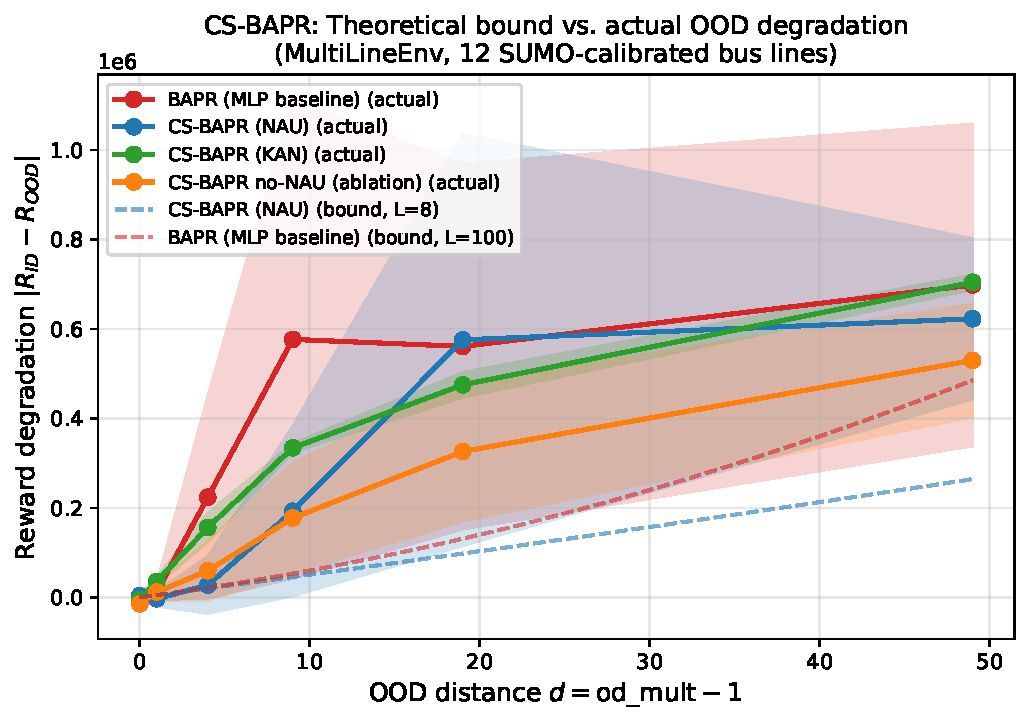
\includegraphics[width=0.82\linewidth]{figures/figure1.pdf}
    \caption{Theory-experiment alignment on the MultiLineEnv benchmark. Markers: measured OOD reward degradation $|R_{\text{ID}} - R_{\text{OOD}}|$ for each method at $d = m - 1 \in \{0, 1, 4, 9, 19, 49\}$, averaged over 3 seeds (shaded: $\pm$s.d.). Dashed curves: theoretical envelope $\delta + (\varepsilon + L_{\text{eff}} d)\,d$ evaluated with representative $L_{\text{eff}}$ values---$L{=}8$ for \texttt{csbapr} (NAU; the envelope is tight) and $L{=}100$ for \texttt{bapr} (a large stand-in for ``ReLU does not admit a finite $L$''). All three CS-BAPR variants stay below the baseline envelope; BAPR escapes into the wide-variance regime characteristic of unbounded derivative drift. Note that the envelope is relative to the policy's own linear reference (no symbolic extension active in these runs), so $\varepsilon$ is the measured ID boundary error.}
    \label{fig:bound}
\end{figure}

\subsection{Additional analysis}

\textbf{Computational cost.} The NAU head adds negligible computational overhead relative to the MLP baseline ($<$5\% wall-clock). The stabilization fixes are $O(1)$ per update. With three seeds and 500 episodes per configuration, a full run completes in approximately 4.5 hours per seed-configuration on a single CPU core; a hardware-aware launcher (\texttt{scripts/run\_smart\_CS-BAPR.sh}) parallelizes across seeds and configurations based on detected CPU/GPU resources.

\textbf{What we do \emph{not} claim.} We do not claim, on this benchmark, that the SINDy or IRM extensions help: we did not activate them in these runs, and the nature of the task (counteracting demand-driven dynamics, not tracking them) is inside the regime where \Cref{sec:scope} predicts they should not help. A benchmark where the symbolic extensions \emph{do} help---a classical tracking task with an analytic optimal control law---is flagged as future work in \Cref{sec:conclusion}.


\section{Conclusion}
\label{sec:conclusion}

This paper presents CS-BAPR, a \emph{family} of methods for OOD extrapolation in reinforcement learning built around two components: (i)~a set of six training-stabilization fixes---four CS-BAPR base fixes (min-$Q$ ensemble targets, running-EMA reward normalization, entropy-temperature floor, and disabling the BAPR behavioural-cloning anchor for constrained heads) plus two ports of BAPR v10/v14 (BOCD-mechanism warmup, penalty-scale tuning, and rollout-based one-sided surprise; see \Cref{sec:training_fixes})---and (ii)~an architecturally-varied actor head chosen from NAU/NMU, KAN, or plain MLP-with-tanh. The theoretical core, machine-verified in Lean~4, is the \emph{OOD Extrapolation Stability Bound} $\|\pi(x_{\text{ood}}) - \pi_{\text{ref}}(x_{\text{ood}})\| \leq \delta + \varepsilon\|d\| + \tfrac{L}{2}\|d\|^2$ (\Cref{thm:ood_quad_nD}) together with the \emph{ReLU Impossibility Theorem} $\nexists L,\ \text{HasArithmeticInductiveBias}(\text{ReLU}, L)$ (\Cref{thm:relu_impossible}) and the \emph{CS-BAPR Bellman contraction} (\Cref{thm:csbapr_contraction}). The bound is instantiable by any of the three CS-BAPR heads (NAU gives $L{=}0$, NMU gives $L{=}2|c|$, KAN and spectrally-normalized MLP give finite bounded $L$) but not by the ReLU baseline.

Empirically, on a 12-line SUMO-calibrated transit holding benchmark evaluated under three OOD protocols (static demand sweep to $50{\times}$, abrupt burst at $t{=}3600$s, within-episode piecewise-constant oscillation with up to 9 switches per episode and peak $50{\times}$), all three CS-BAPR variants outperform the BAPR (ReLU, no fixes) baseline at every OOD cell we measured. The full \texttt{csbapr} configuration (NAU $+$ 6 fixes, $n{=}10$ seeds) is best at in-distribution and at every mid-range OOD cell ($23{-}32\%$ over BAPR at $m{=}5{-}10{\times}$), and best on every within-episode oscillation schedule. \texttt{csbapr-no-nau} (MLP $+$ 6 fixes) ties \texttt{csbapr} within $2\%$ at extreme OOD ($m{=}20{-}50{\times}$) with tighter run-to-run variance. The crash rate (fraction of seeds with $m{=}20{\times}$ return below $-1{,}500$K) drops from $67\%$ for the unstabilized BAPR baseline to $10\%$ for the full \texttt{csbapr} configuration; ablating either the NAU output head or the v14 fix individually raises the residual rate.

The symbolic framework extensions (SINDy-based Jacobian Consistency and IRM causal filtering) are formalized and machine-verified in Lean, but deliberately not activated on this benchmark: transit holding is a counteraction task, not a tracking task, and an early variant including $\Gamma_{\text{sym}}$ under-performed the simpler NAU-only configuration. The extensions are retained as framework-level components for future applications in the tracking regime.

\textbf{Limitations.}
\emph{Architectural scope.} The derivative-Lipschitz bound is specific to bounds of the form $\delta + \varepsilon\|d\| + (L/2)\|d\|^2$; alternative frameworks (e.g., piecewise-linear extrapolation analysis) may yield different guarantees for ReLU networks. Smooth activations (GELU, Softplus, tanh) also admit finite $L$ and are compatible with the bound.
\emph{Training-stabilization fixes carry most of the empirical load.} Our ablation (\texttt{csbapr-no-nau}) isolates the four training-stabilization fixes from the architectural change; the result is that a plain MLP-with-tanh head plus the four fixes already recovers most of the OOD improvement over BAPR. The architectural $L$-bound guarantees from NAU/NMU/KAN are real but do not reliably dominate the MLP-with-fixes variant in our experiments---they trade off ID quality, mid-OOD peak performance, and variance.
\emph{Run-to-run variance on NAU.} In one of three seeds, the NAU actor landed in a poor optimization basin that the $\{-1,0,1\}$ weight constraint could not escape from, yielding an outlier at $m{=}20$. We report the unfiltered mean but flag this as a practical caveat of the constrained-weight architecture.
\emph{Symbolic extensions are optional and domain-restricted.} A benchmark whose optimal policy is an analytic function of state (e.g., energy-shaping pendulum swing-up, LQR tracking) is needed to empirically validate the SINDy extension; this is future work.
\emph{Single benchmark.} The empirical results are on one transit corridor. Generalization across corridors, task structures, and fleet sizes remains to be verified.
\emph{Feature-extractor Lipschitz bound is assumed, not enforced.} Assumption~\ref{assump:feature_lip} requires $L_{\text{feat}} < \infty$; our implementation uses weight clamping, and a principled use of spectral normalization or LipSDP bounds would tighten the composed $L$.

\textbf{Future work.} (i)~Larger-scale seed sweeps ($\geq 10$) to resolve whether NAU's higher variance disappears or persists; (ii)~a tracking-regime benchmark (pendulum swing-up, LQR) to empirically validate the SINDy and IRM extensions; (iii)~principled Lipschitz enforcement on the feature extractor via spectral normalization or LipSDP, which would tighten the composed~$L$; (iv)~online SINDy refinement with formal re-verification of the frozen-parameter condition; and (v)~integrating the CS-BAPR family with distributional RL for risk-sensitive OOD deployment.

\section*{Acknowledgments}
This work was supported by the National Natural Science Foundation of China (Grant No. 72371251), the Natural Science Foundation for Distinguished Young Scholars of Hunan Province (Grant No. 2024JJ2080), and the Key Research and Development Program of Hunan Province of China (Grant No. 2024JK2007).

\input{paper.bbl}
\input{appendix}
\end{document}

\appendix

\section{Lean~4 Proof Overview}
\label{app:lean_overview}

The formal verification is contained in a single file \texttt{CSBAPR.lean} (954~lines, 0~\texttt{sorry}) within the \texttt{proof/CS-BAPR/} directory of the project repository. The file is organized into nine parts:

\begin{center}
\begin{tabular}{clrl}
\toprule
\textbf{Part} & \textbf{Content} & \textbf{Lines} & \textbf{Key Theorem} \\
\midrule
I   & Core definitions                  & 33--57    & \texttt{IsJacobianConsistent}, \texttt{HasArithmeticInductiveBias} \\
II  & 1D OOD extrapolation              & 59--188   & \texttt{scbapr\_ood\_stability\_bound} \\
III & CS-BAPR Bellman contraction        & 189--395  & \texttt{csbapr\_contraction} \\
IV  & Belief update preservation         & 346--386  & \texttt{csbapr\_contraction\_after\_update} \\
V   & $n$-D generalization               & 394--443  & \texttt{scbapr\_ood\_linear\_nD} \\
VI  & SINDy formalization                & 456--595  & \texttt{sindy\_to\_ood\_bound\_nD} \\
VII & $n$-D quadratic OOD bound          & 597--697  & \texttt{scbapr\_ood\_quadratic\_nD} \\
VIII& IRM causal filtering               & 699--774  & \texttt{irm\_to\_ood\_bound\_nD} \\
IX  & NAU/NMU structural guarantees      & 776--953  & \texttt{relu\_derivative\_not\_lipschitz} \\
\bottomrule
\end{tabular}
\end{center}

\noindent The proof relies on Mathlib's calculus library, particularly:
\begin{itemize}
    \item \texttt{norm\_image\_sub\_le\_of\_norm\_deriv\_right\_le\_segment} --- 1D MVT-based segment bound.
    \item \texttt{image\_norm\_le\_of\_norm\_deriv\_right\_le\_deriv\_boundary'} --- Gr\"onwall-style fencing theorem (1D quadratic bound).
    \item \texttt{Convex.norm\_image\_sub\_le\_of\_norm\_fderiv\_le} --- Convex set MVT for $n$-D linear bound.
    \item \texttt{image\_norm\_le\_of\_norm\_deriv\_right\_le\_deriv\_boundary} --- $F$-valued fencing theorem ($n$-D quadratic bound).
\end{itemize}



\section{Complete Proofs}
\label{app:proof_main}

This section provides full mathematical proofs for the key theorems stated in the main text. All proofs are also machine-verified in Lean~4.

\subsection{Proof of Theorem~\ref{thm:ood_1d} (1D OOD Stability Bound)}

\begin{proof}
    Define $e: \mathbb{R} \to \mathbb{R}$ by $e(x) = \pi(x) - f_{\text{real}}(x)$. Since $\pi$ and $f_{\text{real}}$ are differentiable, so is $e$, with $e'(x) = \pi'(x) - f_{\text{real}}'(x)$.

    By hypothesis, $\|e(a)\| \leq \delta$ and $\|e'(x)\| \leq \varepsilon + L(x - a)$ for all $x \in [a, b)$.

    Define the comparison function $g: [a, b] \to \mathbb{R}$ by $g(x) = \delta + \varepsilon(x - a) + \frac{L}{2}(x - a)^2$.

    We verify: (i) $g(a) = \delta \geq \|e(a)\|$; (ii) $g'(x) = \varepsilon + L(x - a) \geq \|e'(x)\|$ for $x \in [a, b)$.

    By the Gr\"onwall-style fencing theorem (for $F$-valued functions with real envelope, formalized in Mathlib as \texttt{image\_norm\_le\_of\_norm\_deriv\_right\_le\_deriv\_boundary'}), we conclude $\|e(x)\| \leq g(x)$ for all $x \in [a, b]$.

    Evaluating at $x = b$: $\|e(b)\| \leq g(b) = \delta + \varepsilon(b - a) + \frac{L}{2}(b - a)^2$.
\end{proof}

\subsection{Proof of Theorem~\ref{thm:ood_linear_nD} ($n$-D Linear Bound)}

\begin{proof}
    Define $e: E \to F$ by $e(x) = \pi(x) - f_{\text{real}}(x)$. Then $De(x) = D\pi(x) - Df_{\text{real}}(x)$, and $\|De(x)\|_{\text{op}} \leq C$ for all $x$ by hypothesis.

    The convex hull of $\{x_0, x_{\text{ood}}\}$ is the line segment $[x_0, x_{\text{ood}}]$, which is convex. By the $n$-dimensional Mean Value Theorem for normed spaces (Mathlib: \texttt{Convex.norm\_image\_sub\_le\_of\_norm\_fderiv\_le}):
    \[
        \|e(x_{\text{ood}}) - e(x_0)\| \leq C \cdot \|x_{\text{ood}} - x_0\|.
    \]
    Triangle inequality:
    \[
        \|e(x_{\text{ood}})\| \leq \|e(x_0)\| + \|e(x_{\text{ood}}) - e(x_0)\| \leq \delta + C\|d\|.
    \]
\end{proof}

\subsection{Proof of Theorem~\ref{thm:ood_quad_nD} ($n$-D Quadratic OOD Bound --- Main Result)}

\begin{proof}
    Let $d = x_{\text{ood}} - x_0$ and parametrize the line segment as $\gamma(t) = x_0 + td$ for $t \in [0, 1]$.

    Define the pullback error function $e_{\text{path}}: [0, 1] \to F$ by $e_{\text{path}}(t) = \pi(\gamma(t)) - f_{\text{real}}(\gamma(t))$.

    \textbf{Step 1 (Boundary condition):} $\|e_{\text{path}}(0)\| = \|\pi(x_0) - f_{\text{real}}(x_0)\| \leq \delta$.

    \textbf{Step 2 (Derivative bound):} By the chain rule, $e_{\text{path}}'(t) = (D\pi(\gamma(t)) - Df_{\text{real}}(\gamma(t))) \cdot d$, so $\|e_{\text{path}}'(t)\| \leq \|D\pi(\gamma(t)) - Df_{\text{real}}(\gamma(t))\| \cdot \|d\|$. By hypothesis~(ii), this is bounded by $\varepsilon\|d\| + L\|d\|^2 \cdot t$.

    \textbf{Step 3 (Fencing):} Define the comparison function $g(t) = \delta + \varepsilon\|d\| \cdot t + \frac{L\|d\|^2}{2} \cdot t^2$ with $g(0) = \delta \geq \|e_{\text{path}}(0)\|$ and $g'(t) = \varepsilon\|d\| + L\|d\|^2 t \geq \|e_{\text{path}}'(t)\|$. By the fencing theorem (Mathlib: \texttt{image\_norm\_le\_of\_norm\_deriv\_right\_le\_deriv\_boundary}), $\|e_{\text{path}}(t)\| \leq g(t)$ for all $t \in [0, 1]$.

    \textbf{Step 4 (Evaluation):} $\|e_{\text{path}}(1)\| \leq g(1) = \delta + \varepsilon\|d\| + \frac{L}{2}\|d\|^2$. Since $\gamma(1) = x_{\text{ood}}$, this gives $\|\pi(x_{\text{ood}}) - f_{\text{real}}(x_{\text{ood}})\| \leq \delta + \varepsilon\|d\| + \frac{L}{2}\|d\|^2$.
\end{proof}

\subsection{Proof of Theorem~\ref{thm:csbapr_contraction} (CS-BAPR Contraction)}

\begin{proof}
    Fix $Q_1, Q_2$ with $\|Q_1 - Q_2\|_\infty \leq \varepsilon$. For each mode $h$ and state-action $(s, a)$:
    \begin{align*}
        &|\mathcal{T}_h^{CS} Q_1(s,a) - \mathcal{T}_h^{CS} Q_2(s,a)| \\
        &= \gamma \left|\sum_{s'} P_h(s'|s,a)(V^{Q_1}(s') - V^{Q_2}(s'))\right|
    \end{align*}
    where the frozen penalty terms ($\Gamma_{\text{epi}}^h$, $\Gamma_{\text{sym}}^h$, $\kappa_{\text{ale}}$) cancel exactly because they do not depend on $Q_1$ or $Q_2$.

    Since $|V^{Q_1}(s') - V^{Q_2}(s')| \leq \|Q_1 - Q_2\|_\infty = \varepsilon$ and $\sum_{s'} P_h(s'|s,a) = 1$:
    \[
        |\mathcal{T}_h^{CS} Q_1(s,a) - \mathcal{T}_h^{CS} Q_2(s,a)| \leq \gamma \varepsilon.
    \]

    For the belief-weighted mixture: $|\mathcal{T}_\rho^{CS} Q_1(s,a) - \mathcal{T}_\rho^{CS} Q_2(s,a)| \leq \sum_h \rho(h) \cdot \gamma\varepsilon = \gamma\varepsilon$ since $\sum_h \rho(h) = 1$. Taking the supremum over $(s,a)$ gives $\|\mathcal{T}_\rho^{CS} Q_1 - \mathcal{T}_\rho^{CS} Q_2\|_\infty \leq \gamma \varepsilon = \gamma\|Q_1 - Q_2\|_\infty$. Banach's fixed-point theorem gives the unique fixed point.
\end{proof}


\section{Remaining Proofs}
\label{app:lean_statements}

This section provides proofs for theorems stated in the main text that were not covered in Appendix~\ref{app:proof_main}. Each proof is paired with its Lean~4 cross-reference.

\subsection{Proof of Lemma~\ref{lem:error_linear} (Linear Error Growth)}

\begin{proof}
    Define $e(x) = \pi(x) - f_{\text{real}}(x)$. Then $e'(x) = \pi'(x) - f_{\text{real}}'(x)$ and $\|e'(x)\| \leq C$ for $x \in [a, b)$.
    Apply Mathlib's segment MVT (\texttt{norm\_image\_sub\_le\_of\_norm\_deriv\_right\_le\_segment}) to $e$ on $[a, b]$:
    \[
        \|e(b) - e(a)\| \leq C \cdot (b - a).
    \]
    Expanding: $\|(\pi(b) - f_{\text{real}}(b)) - (\pi(a) - f_{\text{real}}(a))\| \leq C(b - a)$.

    \noindent\textit{Lean:} \texttt{error\_growth\_linear}, line~65.
\end{proof}

\subsection{Proof of Lemma~\ref{lem:path_fencing} (Path-Level Fencing)}

\begin{proof}
    $e_{\text{path}}: [0,1] \to F$ satisfies $\|e_{\text{path}}(0)\| \leq \delta$ and $\|e_{\text{path}}'(t)\| \leq \varepsilon_d + L_d \cdot t$ for $t \in [0,1)$.

    Define the comparison function $g(t) = \delta + \varepsilon_d \cdot t + \frac{L_d}{2} t^2$. Then $g(0) = \delta \geq \|e_{\text{path}}(0)\|$ and $g'(t) = \varepsilon_d + L_d \cdot t \geq \|e_{\text{path}}'(t)\|$.

    By Mathlib's fencing theorem (\texttt{image\_norm\_le\_of\_norm\_deriv\_right\_le\_deriv\_boundary}), $\|e_{\text{path}}(t)\| \leq g(t)$ for all $t \in [0,1]$.

    Evaluating at $t = 1$: $\|e_{\text{path}}(1)\| \leq \delta + \varepsilon_d + L_d / 2$.

    \noindent\textit{Lean:} \texttt{scbapr\_ood\_quadratic\_path}, line~629.
\end{proof}

\subsection{Proof of Theorem~\ref{thm:nau_const} (NAU Derivative Constancy)}

\begin{proof}
    NAU computes $y = \sum_j w_j x_j$, so $\partial y / \partial x_i = w_i$ for all input vectors $x$. Since $w_i$ is a fixed integer weight (independent of $x$), the derivative function $x \mapsto w_i$ is constant. Formally, $\text{deriv}(\lambda x_i.\, \sum_j w_j x_j, i) = \lambda \_.\ w_i$.

    \noindent\textit{Lean:} \texttt{nau\_derivative\_is\_constant}, line~817.
\end{proof}

\subsection{Proof of Corollary~\ref{cor:sindy_tight} (Tight SINDy Consistency)}

\begin{proof}
    When the same coefficient set $\xi$ is used both for SINDy identification and for training, the triangle inequality gives: $\|D\pi(x) - Df_{\text{real}}(x)\| \leq \|D\pi(x) - Df_{\text{sym}}(x)\| + \|Df_{\text{sym}}(x) - Df_{\text{real}}(x)\| \leq \varepsilon_2 + \varepsilon_1$.
        This is the same bound as Theorem~\ref{thm:sindy_jac} but with the explicit requirement that both error measurements use the same $f_{\text{sym}} = \sum_i \xi_i \varphi_i$.

    \noindent\textit{Lean:} \texttt{sindy\_implies\_jacobian\_consistency\_tight}, line~546.
\end{proof}

\subsection{Proof of Theorem~\ref{thm:irm_pipeline} (Full IRM-to-OOD Pipeline)}

\begin{proof}
    Compose in three steps:
    \begin{enumerate}
        \item By IRM Consistency, $\forall x,\ \|Df_{\text{real}}^e(x) - Df_{\text{sym}}(x)\| \leq \varepsilon_{\text{irm}}$ in environment $e$.
        \item By the training bound, $\forall x,\ \|D\pi(x) - Df_{\text{sym}}(x)\| \leq \varepsilon_{\text{pol}}$.
        \item Triangle inequality: $\|D\pi(x) - Df_{\text{real}}^e(x)\| \leq \varepsilon_{\text{irm}} + \varepsilon_{\text{pol}}$.
    \end{enumerate}
    This gives $(\varepsilon_{\text{irm}} + \varepsilon_{\text{pol}})$-Jacobian Consistency with $f_{\text{real}}^e$.
    Setting $C = \varepsilon_{\text{irm}} + \varepsilon_{\text{pol}}$ in the $n$-D linear OOD bound (Theorem~\ref{thm:ood_linear_nD}):
    \[
        \|\pi(x_{\text{ood}}) - f_{\text{real}}^e(x_{\text{ood}})\| \leq \delta + (\varepsilon_{\text{irm}} + \varepsilon_{\text{pol}})\|x_{\text{ood}} - x_0\|.
    \]

    \noindent\textit{Lean:} \texttt{irm\_to\_ood\_bound\_nD}, line~755.
\end{proof}

\subsection{Proof of Corollary 4.12 (Contraction After Belief Update)}

\begin{proof}
    After Bayesian update, $\rho'(h) = \rho(h) \cdot L(h) / Z$ where $L(h) \geq 0$ and $Z = \sum_h \rho(h) L(h) > 0$.

    Since $\rho(h) \geq 0$ and $L(h) \geq 0$, we have $\rho'(h) \geq 0$. Since $\sum_h \rho'(h) = \sum_h \rho(h) L(h) / Z = Z / Z = 1$, $\rho'$ is a valid probability distribution.

    The proof of Theorem~\ref{thm:csbapr_contraction} only requires $\rho(h) \geq 0$ and $\sum_h \rho(h) = 1$. Since $\rho'$ satisfies both conditions, $\mathcal{T}_{\rho'}^{CS\text{-}BAPR}$ is a $\gamma$-contraction.

    \noindent\textit{Lean:} \texttt{csbapr\_contraction\_after\_update}, line~370.
\end{proof}


\section{CS-BAPR Operator: Detailed Derivation}
\label{app:operator_detail}

\subsection{Relationship to BAPR and RE-SAC operators}

The CS-BAPR mode-conditional operator (Eq.~\eqref{eq:csbapr_mode}) extends the BAPR operator with a single additional frozen penalty term $\lambda_{\text{sym}} \cdot \Gamma_{\text{sym}}^h(s,a)$:

\begin{center}
\begin{tabular}{llc}
\toprule
\textbf{Penalty} & \textbf{Source} & \textbf{Origin} \\
\midrule
$\kappa_{\text{ale}} = \lambda_{\text{ale}} \sum_l \|W_l\|_1$ & Frozen target critic weights & RE-SAC \\
$\Gamma_{\text{epi}}^h(s,a) = \text{Var}(\{Q_{\phi'_k}\})$ & Frozen target Q-ensemble & RE-SAC \\
$\rho(h)$ belief weights & Frozen BOCD posterior & BAPR \\
$\Gamma_{\text{sym}}^h(s,a) = \|\nabla_s \pi - \nabla_s f_{\text{sym}}\|^2$ & Frozen SINDy coefficients & \textbf{CS-BAPR} \\
\bottomrule
\end{tabular}
\end{center}

\subsection{Why $\Gamma_{\text{sym}}$ cancels in contraction}

In the contraction argument (Lean: \texttt{t\_mode\_pointwise\_bound}, line~251), all terms that do not depend on the Q-function being evaluated cancel:
\begin{align}
    &\mathcal{T}_h^{CS} Q_1(s,a) - \mathcal{T}_h^{CS} Q_2(s,a) \notag \\
    &= \gamma \sum_{s'} P_h(s'|s,a) \left[ V^{Q_1}(s') - V^{Q_2}(s') \right] \notag \\
    &\quad \underbrace{- \lambda_{\text{epi}}\Gamma_{\text{epi}}^h + \lambda_{\text{epi}}\Gamma_{\text{epi}}^h}_{= 0} \underbrace{- \lambda_{\text{sym}}\Gamma_{\text{sym}}^h + \lambda_{\text{sym}}\Gamma_{\text{sym}}^h}_{= 0} \underbrace{- \kappa + \kappa}_{= 0}.
\end{align}
The cancellation requires that $\Gamma_{\text{sym}}$ is \emph{identical} in both $\mathcal{T}_h^{CS} Q_1$ and $\mathcal{T}_h^{CS} Q_2$, which holds precisely because the SINDy coefficients are frozen (not updated based on Q).

\subsection{Frozen-parameter requirement for $\Gamma_{\text{sym}}$}

In the implementation, $f_{\text{sym}}$ is a \texttt{SINDyTorchWrapper} whose coefficients are stored as non-trainable buffers (\texttt{register\_buffer}). The SINDy gradients are \texttt{detach()}-ed in the Jacobian loss computation:
\begin{equation}
    \Gamma_{\text{sym}} = \|\nabla_s \pi_\theta(s) - \underbrace{\nabla_s f_{\text{sym}}(s)}_{\text{detached}}\|^2.
\end{equation}
This ensures that $\Gamma_{\text{sym}}$ depends on the current policy parameters $\theta$ (through $\nabla_s \pi_\theta$) but \emph{not} on the Q-function being updated, satisfying the frozen-parameter condition.


\section{SINDy Implementation Details}
\label{app:sindy_details}

\subsection{State derivative estimation}

SINDy requires state derivatives $\dot{X} = ds/dt$. In the RL setting, we only observe discrete transitions $(s_t, a_t, s_{t+1})$. We use first-order finite differences:
\begin{equation}
    \dot{s}_t \approx \frac{s_{t+1} - s_t}{\Delta t},
\end{equation}
where $\Delta t$ is the environment timestep. For discrete-time SINDy (our default), we directly model $s_{t+1} = f(s_t)$, avoiding derivative estimation entirely.

\subsection{SINDy-to-PyTorch bridge}

The SINDy model (fitted via PySINDy in NumPy) is converted to a differentiable PyTorch module by reconstructing the polynomial basis function computation in PyTorch:
\begin{equation}
    f_{\text{sym}}(x) = \Theta(x) \cdot \xi^T,
\end{equation}
where $\Theta(x)$ is the polynomial library matrix and $\xi$ are the frozen SINDy coefficients stored as \texttt{register\_buffer}. This enables automatic differentiation for the Jacobian Consistency Loss without backpropagating through the SINDy coefficients.

\subsection{Quality verification}

Before proceeding to Phase~1 training, we verify the SINDy quality gate:
\begin{equation}
    \varepsilon_1 = \frac{1}{|D_{\text{test}}|} \sum_{x \in D_{\text{test}}} \|Df_{\text{real}}(x) - Df_{\text{sym}}(x)\| < \varepsilon_{\text{threshold}}.
\end{equation}
If SINDy fails this gate, the basis library degree is increased or additional exploration data is collected.


\section{NAU/NMU Architecture Details}
\label{app:nau_details}

\subsection{NAU weight discretization}

NAU layers use clamped real-valued weights with a sparsity regularizer that drives weights toward $\{-1, 0, 1\}$:
\begin{equation}
    \mathcal{L}_{\text{NAU}} = \sum_i \min(|w_i|, |1 - |w_i||).
\end{equation}
This is a continuous relaxation following Madsen \& Johansen~\cite{Madsen2020NAU}, where $w_i \in [-1, 1]$ via clamping and the regularizer encourages convergence to the discrete set.

\subsection{Actor architecture}

The CS-BAPR actor combines a standard feature extractor (2-layer MLP with LeakyReLU) with NAU/NMU output heads:
\begin{align}
    h &= \text{LeakyReLU}(W_2 \cdot \text{LeakyReLU}(W_1 \cdot s)), \\
    a_{\text{linear}} &= \text{NAU}(h), \quad L = 0, \\
    a_{\text{quad}} &= \text{NMU}(\text{Linear}(h)), \quad L = 2|c|, \\
    a &= \tanh(\alpha \cdot a_{\text{linear}} + (1-\alpha) \cdot a_{\text{quad}}),
\end{align}
where $\alpha \in [0,1]$ is a learnable mixing coefficient.

\subsection{Effective Lipschitz derivative constant $L_{\text{eff}}$}
\label{app:leff}

The effective Lipschitz derivative constant of the composed actor is bounded by:
\begin{equation}
    L_{\text{eff}} \leq L_{\text{feat}} \cdot L_{\text{head}} \cdot L_{\tanh},
\end{equation}
where each factor corresponds to a composition stage:
\begin{itemize}
    \item $L_{\text{feat}}$: The feature extractor's Lipschitz constant. For bounded-weight networks with LeakyReLU activations (slope $\alpha_\ell > 0$), this is finite: LeakyReLU is globally Lipschitz with constant $\max(1, \alpha_\ell) = 1$, so $L_{\text{feat}} \leq \prod_l \|W_l\|_{\text{op}}$. This is controlled via weight clamping inherited from the NAU regularizer.

    \item $L_{\text{head}} = \alpha \cdot 0 + (1-\alpha) \cdot 2|c| = 2(1-\alpha)|c|$: The output head's derivative Lipschitz constant, which is a convex combination of NAU ($L=0$) and NMU ($L=2|c|$).

    \item $L_{\tanh} \leq 1$: Since $|\tanh'(x)| \leq 1$ everywhere, the tanh activation does not amplify the Lipschitz constant.
\end{itemize}

Crucially, the LeakyReLU feature layers contribute a \emph{finite} $L_{\text{feat}}$ (unlike ReLU, whose derivative is discontinuous at 0). The composed $L_{\text{eff}}$ is therefore finite, preserving the quadratic OOD bound, albeit with a potentially larger constant than the isolated NAU/NMU proofs suggest. The constant can be further tightened via spectral normalization~\cite{Madsen2020NAU} or LipSDP methods.


\section{IRM Filtering Protocol}
\label{app:irm_protocol}

\subsection{Multi-environment setup}

IRM filtering requires at least $K \geq 3$ training environments with distinct dynamics parameters but shared causal structure. For each environment $e_k$:
\begin{enumerate}
    \item Collect exploration trajectories $\{(s_t^k, a_t^k, s_{t+1}^k)\}$.
    \item Fit SINDy independently: $\xi_k = \text{SINDy}(X^k, \dot{X}^k)$.
    \item Evaluate cross-environment derivative error variance:
    \begin{equation}
        V_{\text{IRM}} = \text{Var}_{k} \left[ \frac{1}{|D_k|} \sum_{x \in D_k} \|Df_{\text{real}}^k(x) - Df_{\text{sym}}(x)\| \right].
    \end{equation}
\end{enumerate}

\subsection{Formula selection}

The IRM-selected formula minimizes cross-environment variance:
\begin{equation}
    \xi_{\text{irm}} = \arg\min_{\xi \in \{\xi_1, \ldots, \xi_K\}} V_{\text{IRM}}(\xi).
\end{equation}
By Theorem~\ref{thm:irm_tighten}, this yields $\varepsilon_{\text{irm}} \leq \varepsilon_{\text{raw}}$, tightening the OOD bound.


\section{Hyperparameter Configuration}
\label{app:hyperparams}

\begin{table}[H]
\caption{CS-BAPR hyperparameters. Inherited parameters from BAPR are marked with $\dagger$.}
\label{tab:hyperparams}
\centering
\begin{tabular}{llll}
\toprule
\textbf{Parameter} & \textbf{Symbol} & \textbf{Default} & \textbf{Lean constraint} \\
\midrule
\multicolumn{4}{l}{\textit{SAC core (inherited$^\dagger$)}} \\
Discount factor$^\dagger$ & $\gamma$ & 0.99 & $0 \leq \gamma < 1$ \\
Soft update rate$^\dagger$ & $\tau$ & 0.005 & --- \\
Entropy coefficient$^\dagger$ & $\alpha$ & auto-tuned & --- \\
Learning rates$^\dagger$ & $\eta$ & $3 \times 10^{-4}$ & --- \\
Ensemble size$^\dagger$ & $K$ & 5 & --- \\
Batch size$^\dagger$ & $B$ & 256 & --- \\
\midrule
\multicolumn{4}{l}{\textit{BAPR inherited$^\dagger$}} \\
Max run length$^\dagger$ & $H$ & 20 & --- \\
Hazard rate$^\dagger$ & $H_{\text{hazard}}$ & 0.02 & --- \\
Epistemic weight$^\dagger$ & $\lambda_{\text{epi}}$ & 0.01 & $\geq 0$ \\
OOD penalty$^\dagger$ & $\beta_{\text{ood}}$ & 0.1 & --- \\
\midrule
\multicolumn{4}{l}{\textit{CS-BAPR new}} \\
Symbolic weight & $\lambda_{\text{sym}}$ & 0.01 & $\geq 0$ \\
Jacobian weight & $\mu_{\text{jac}}$ & 0.1 & --- \\
Gradient clipping & --- & 1.0 & --- \\
SINDy threshold & --- & 0.1 & --- \\
SINDy library degree & --- & 2 & --- \\
NAU regularization & --- & 0.01 & --- \\
IRM penalty weight & --- & 0.1 & --- \\
\bottomrule
\end{tabular}
\end{table}


\section{Proof Sketch: Component Hypotheses Imply Derivative Bound}
\label{app:component_lemma}

Lemma \texttt{deriv\_error\_bound\_from\_components} (line~157) shows how the three CS-BAPR components combine to satisfy the derivative bound hypothesis of the main theorem:

\begin{lemma}
    If the real dynamics $f_{\text{real}}$ has constant derivative (smooth physical law), the policy is $\varepsilon$-Jacobian Consistent at the training boundary $a$, and has $L$-Arithmetic Inductive Bias, then:
    \begin{equation}
        \forall x,\quad |(\pi'(x) - f_{\text{real}}'(x))| \leq \varepsilon + L|x - a|.
    \end{equation}
\end{lemma}

\begin{proof}
    By triangle inequality:
    \begin{align}
        |\pi'(x) - f_{\text{real}}'(x)| &= |(\pi'(x) - \pi'(a)) + (\pi'(a) - f_{\text{real}}'(a))| \\
        &\leq |\pi'(x) - \pi'(a)| + |\pi'(a) - f_{\text{real}}'(a)| \\
        &\leq L|x - a| + \varepsilon,
    \end{align}
    where the first term uses the Lipschitz derivative property (NAU/NMU) and the second uses Jacobian Consistency at $a$ (SINDy training). The constant-derivative assumption on $f_{\text{real}}$ ensures $f_{\text{real}}'(a) = f_{\text{real}}'(x)$.
\end{proof}

This lemma provides the formal bridge from CS-BAPR's three architectural/training assumptions to the hypothesis required by Theorem~\ref{thm:ood_1d}.


\section{Formalization: Data Structure Design}
\label{app:lean_structures}

This section documents the Lean~4 data structures used to formalize CS-BAPR, explaining the mathematical rationale behind each design choice.

\subsection{NAU Layer}

\begin{definition}[NAU Layer, Lean line~799]
    An NAU layer of dimension $n$ is a weight vector $w \in \{-1, 0, 1\}^n$ computing $y = \sum_{j=1}^n w_j x_j$.
\end{definition}

The discreteness constraint $w_i \in \{-1, 0, 1\}$ is essential: it ensures that the NAU computes an \emph{exact} integer linear combination, making the derivative $\partial y / \partial x_i = w_i$ trivially constant (Theorem~\ref{thm:nau_const}). Without discreteness, the NAU would be a general linear layer with no structural advantage over standard networks. In the Lean formalization, this is encoded as:
\begin{center}
\fbox{\parbox{0.92\linewidth}{\small\ttfamily
structure NAULayer (n : $\mathbb{N}$) where\\
\quad weights : Fin n $\to$ $\mathbb{Z}$\\
\quad weight\_discrete : $\forall$ i, weights i = -1 $\lor$ weights i = 0 $\lor$ weights i = 1
}}
\end{center}

\subsection{SINDy Coefficients and Reconstruction}

\begin{definition}[SINDy Coefficients, Lean line~470]
    Given a basis library $\{\varphi_1, \ldots, \varphi_n\}$, SINDy coefficients are a vector $\xi \in \mathbb{R}^n$ defining the symbolic formula $f_{\text{sym}}(x) = \sum_{i=1}^n \xi_i \varphi_i(x)$.
\end{definition}

The \texttt{reconstruct} function maps coefficients back to the function space, enabling direct comparison with $\pi$ and $f_{\text{real}}$. The Fr\'echet derivative of the reconstruction is $Df_{\text{sym}}(x) = \sum_i \xi_i D\varphi_i(x)$, which is used in the Jacobian Consistency definition (Definition~\ref{def:jac_consistency}). In Lean:
\begin{center}
\fbox{\parbox{0.92\linewidth}{\small\ttfamily
structure SINDyCoeffs (n : $\mathbb{N}$) where\\
\quad vals : Fin n $\to$ $\mathbb{R}$\\
\\
def SINDyCoeffs.reconstruct (c : SINDyCoeffs n) (lib : BasisLibrary n E F) : E $\to$ F :=\\
\quad fun x $\Rightarrow$ $\sum$ i, c.vals i $\bullet$ lib.basis i x
}}
\end{center}

\subsection{IRM Environment}

\begin{definition}[Environment, Lean line~715]
    An environment consists of a training domain $D_{\text{train}} \subseteq E$ and a ground-truth response function $f_{\text{real}}: E \to F$.
\end{definition}

IRM filtering (Pillar~III) requires comparing symbolic formulas across \emph{multiple} environments. Each environment shares the same state/action spaces but has distinct dynamics parameters (e.g., different masses, friction coefficients). The IRM Consistency predicate (Definition~\ref{def:irm}) requires that a single SINDy coefficient vector $\xi$ achieves low derivative error \emph{simultaneously} across all environments in the list, ensuring causal rather than spurious correlation. In Lean:
\begin{center}
\fbox{\parbox{0.92\linewidth}{\small\ttfamily
structure Environment (E F : Type*)\\
\quad[NormedAddCommGroup E] [NormedSpace $\mathbb{R}$ E]\\
\quad[NormedAddCommGroup F] [NormedSpace $\mathbb{R}$ F] where\\
\quad D\_train : Set E\\
\quad f\_real : E $\to$ F
}}
\end{center}

\subsection{NMU Unit}

\begin{definition}[NMU Unit, Lean line~858]
    An NMU unit with coefficient $c \in \mathbb{R}$ computes $f(x) = cx^2$.
\end{definition}

The single-parameter design is deliberate: the NMU's second derivative is $f''(x) = 2c$ (constant), yielding the exact Lipschitz constant $L = 2|c|$ for the first derivative (Theorem~\ref{thm:nmu_bias}). Richer polynomial units (e.g., $f(x) = c_1 x^2 + c_2 x^3$) would have \emph{non-constant} second derivatives, making the Lipschitz constant depend on the input domain and losing the global guarantee. In Lean:
\begin{center}
\fbox{\parbox{0.92\linewidth}{\small\ttfamily
structure NMUUnit where\\
\quad coeff : $\mathbb{R}$
}}
\end{center}

\end{document}

\appendix

\section{Lean~4 Proof Overview}
\label{app:lean_overview}

The formal verification is contained in a single file \texttt{CSBAPR.lean} (954~lines, 0~\texttt{sorry}) within the \texttt{proof/CS-BAPR/} directory of the project repository. The file is organized into nine parts:

\begin{center}
\begin{tabular}{clrl}
\toprule
\textbf{Part} & \textbf{Content} & \textbf{Lines} & \textbf{Key Theorem} \\
\midrule
I   & Core definitions                  & 33--57    & \texttt{IsJacobianConsistent}, \texttt{HasArithmeticInductiveBias} \\
II  & 1D OOD extrapolation              & 59--188   & \texttt{scbapr\_ood\_stability\_bound} \\
III & CS-BAPR Bellman contraction        & 189--395  & \texttt{csbapr\_contraction} \\
IV  & Belief update preservation         & 346--386  & \texttt{csbapr\_contraction\_after\_update} \\
V   & $n$-D generalization               & 394--443  & \texttt{scbapr\_ood\_linear\_nD} \\
VI  & SINDy formalization                & 456--595  & \texttt{sindy\_to\_ood\_bound\_nD} \\
VII & $n$-D quadratic OOD bound          & 597--697  & \texttt{scbapr\_ood\_quadratic\_nD} \\
VIII& IRM causal filtering               & 699--774  & \texttt{irm\_to\_ood\_bound\_nD} \\
IX  & NAU/NMU structural guarantees      & 776--953  & \texttt{relu\_derivative\_not\_lipschitz} \\
\bottomrule
\end{tabular}
\end{center}

\noindent The proof relies on Mathlib's calculus library, particularly:
\begin{itemize}
    \item \texttt{norm\_image\_sub\_le\_of\_norm\_deriv\_right\_le\_segment} --- 1D MVT-based segment bound.
    \item \texttt{image\_norm\_le\_of\_norm\_deriv\_right\_le\_deriv\_boundary'} --- Gr\"onwall-style fencing theorem (1D quadratic bound).
    \item \texttt{Convex.norm\_image\_sub\_le\_of\_norm\_fderiv\_le} --- Convex set MVT for $n$-D linear bound.
    \item \texttt{image\_norm\_le\_of\_norm\_deriv\_right\_le\_deriv\_boundary} --- $F$-valued fencing theorem ($n$-D quadratic bound).
\end{itemize}



\section{Complete Proofs}
\label{app:proof_main}

This section provides full mathematical proofs for the key theorems stated in the main text. All proofs are also machine-verified in Lean~4.

\subsection{Proof of Theorem~\ref{thm:ood_1d} (1D OOD Stability Bound)}

\begin{proof}
    Define $e: \mathbb{R} \to \mathbb{R}$ by $e(x) = \pi(x) - f_{\text{real}}(x)$. Since $\pi$ and $f_{\text{real}}$ are differentiable, so is $e$, with $e'(x) = \pi'(x) - f_{\text{real}}'(x)$.

    By hypothesis, $\|e(a)\| \leq \delta$ and $\|e'(x)\| \leq \varepsilon + L(x - a)$ for all $x \in [a, b)$.

    Define the comparison function $g: [a, b] \to \mathbb{R}$ by $g(x) = \delta + \varepsilon(x - a) + \frac{L}{2}(x - a)^2$.

    We verify: (i) $g(a) = \delta \geq \|e(a)\|$; (ii) $g'(x) = \varepsilon + L(x - a) \geq \|e'(x)\|$ for $x \in [a, b)$.

    By the Gr\"onwall-style fencing theorem (for $F$-valued functions with real envelope, formalized in Mathlib as \texttt{image\_norm\_le\_of\_norm\_deriv\_right\_le\_deriv\_boundary'}), we conclude $\|e(x)\| \leq g(x)$ for all $x \in [a, b]$.

    Evaluating at $x = b$: $\|e(b)\| \leq g(b) = \delta + \varepsilon(b - a) + \frac{L}{2}(b - a)^2$.
\end{proof}

\subsection{Proof of Theorem~\ref{thm:ood_linear_nD} ($n$-D Linear Bound)}

\begin{proof}
    Define $e: E \to F$ by $e(x) = \pi(x) - f_{\text{real}}(x)$. Then $De(x) = D\pi(x) - Df_{\text{real}}(x)$, and $\|De(x)\|_{\text{op}} \leq C$ for all $x$ by hypothesis.

    The convex hull of $\{x_0, x_{\text{ood}}\}$ is the line segment $[x_0, x_{\text{ood}}]$, which is convex. By the $n$-dimensional Mean Value Theorem for normed spaces (Mathlib: \texttt{Convex.norm\_image\_sub\_le\_of\_norm\_fderiv\_le}):
    \[
        \|e(x_{\text{ood}}) - e(x_0)\| \leq C \cdot \|x_{\text{ood}} - x_0\|.
    \]
    Triangle inequality:
    \[
        \|e(x_{\text{ood}})\| \leq \|e(x_0)\| + \|e(x_{\text{ood}}) - e(x_0)\| \leq \delta + C\|d\|.
    \]
\end{proof}

\subsection{Proof of Theorem~\ref{thm:ood_quad_nD} ($n$-D Quadratic OOD Bound --- Main Result)}

\begin{proof}
    Let $d = x_{\text{ood}} - x_0$ and parametrize the line segment as $\gamma(t) = x_0 + td$ for $t \in [0, 1]$.

    Define the pullback error function $e_{\text{path}}: [0, 1] \to F$ by $e_{\text{path}}(t) = \pi(\gamma(t)) - f_{\text{real}}(\gamma(t))$.

    \textbf{Step 1 (Boundary condition):} $\|e_{\text{path}}(0)\| = \|\pi(x_0) - f_{\text{real}}(x_0)\| \leq \delta$.

    \textbf{Step 2 (Derivative bound):} By the chain rule, $e_{\text{path}}'(t) = (D\pi(\gamma(t)) - Df_{\text{real}}(\gamma(t))) \cdot d$, so $\|e_{\text{path}}'(t)\| \leq \|D\pi(\gamma(t)) - Df_{\text{real}}(\gamma(t))\| \cdot \|d\|$. By hypothesis~(ii), this is bounded by $\varepsilon\|d\| + L\|d\|^2 \cdot t$.

    \textbf{Step 3 (Fencing):} Define the comparison function $g(t) = \delta + \varepsilon\|d\| \cdot t + \frac{L\|d\|^2}{2} \cdot t^2$ with $g(0) = \delta \geq \|e_{\text{path}}(0)\|$ and $g'(t) = \varepsilon\|d\| + L\|d\|^2 t \geq \|e_{\text{path}}'(t)\|$. By the fencing theorem (Mathlib: \texttt{image\_norm\_le\_of\_norm\_deriv\_right\_le\_deriv\_boundary}), $\|e_{\text{path}}(t)\| \leq g(t)$ for all $t \in [0, 1]$.

    \textbf{Step 4 (Evaluation):} $\|e_{\text{path}}(1)\| \leq g(1) = \delta + \varepsilon\|d\| + \frac{L}{2}\|d\|^2$. Since $\gamma(1) = x_{\text{ood}}$, this gives $\|\pi(x_{\text{ood}}) - f_{\text{real}}(x_{\text{ood}})\| \leq \delta + \varepsilon\|d\| + \frac{L}{2}\|d\|^2$.
\end{proof}

\subsection{Proof of Theorem~\ref{thm:csbapr_contraction} (CS-BAPR Contraction)}

\begin{proof}
    Fix $Q_1, Q_2$ with $\|Q_1 - Q_2\|_\infty \leq \varepsilon$. For each mode $h$ and state-action $(s, a)$:
    \begin{align*}
        &|\mathcal{T}_h^{CS} Q_1(s,a) - \mathcal{T}_h^{CS} Q_2(s,a)| \\
        &= \gamma \left|\sum_{s'} P_h(s'|s,a)(V^{Q_1}(s') - V^{Q_2}(s'))\right|
    \end{align*}
    where the frozen penalty terms ($\Gamma_{\text{epi}}^h$, $\Gamma_{\text{sym}}^h$, $\kappa_{\text{ale}}$) cancel exactly because they do not depend on $Q_1$ or $Q_2$.

    Since $|V^{Q_1}(s') - V^{Q_2}(s')| \leq \|Q_1 - Q_2\|_\infty = \varepsilon$ and $\sum_{s'} P_h(s'|s,a) = 1$:
    \[
        |\mathcal{T}_h^{CS} Q_1(s,a) - \mathcal{T}_h^{CS} Q_2(s,a)| \leq \gamma \varepsilon.
    \]

    For the belief-weighted mixture: $|\mathcal{T}_\rho^{CS} Q_1(s,a) - \mathcal{T}_\rho^{CS} Q_2(s,a)| \leq \sum_h \rho(h) \cdot \gamma\varepsilon = \gamma\varepsilon$ since $\sum_h \rho(h) = 1$. Taking the supremum over $(s,a)$ gives $\|\mathcal{T}_\rho^{CS} Q_1 - \mathcal{T}_\rho^{CS} Q_2\|_\infty \leq \gamma \varepsilon = \gamma\|Q_1 - Q_2\|_\infty$. Banach's fixed-point theorem gives the unique fixed point.
\end{proof}


\section{Remaining Proofs}
\label{app:lean_statements}

This section provides proofs for theorems stated in the main text that were not covered in Appendix~\ref{app:proof_main}. Each proof is paired with its Lean~4 cross-reference.

\subsection{Proof of Lemma~\ref{lem:error_linear} (Linear Error Growth)}

\begin{proof}
    Define $e(x) = \pi(x) - f_{\text{real}}(x)$. Then $e'(x) = \pi'(x) - f_{\text{real}}'(x)$ and $\|e'(x)\| \leq C$ for $x \in [a, b)$.
    Apply Mathlib's segment MVT (\texttt{norm\_image\_sub\_le\_of\_norm\_deriv\_right\_le\_segment}) to $e$ on $[a, b]$:
    \[
        \|e(b) - e(a)\| \leq C \cdot (b - a).
    \]
    Expanding: $\|(\pi(b) - f_{\text{real}}(b)) - (\pi(a) - f_{\text{real}}(a))\| \leq C(b - a)$.

    \noindent\textit{Lean:} \texttt{error\_growth\_linear}, line~65.
\end{proof}

\subsection{Proof of Lemma~\ref{lem:path_fencing} (Path-Level Fencing)}

\begin{proof}
    $e_{\text{path}}: [0,1] \to F$ satisfies $\|e_{\text{path}}(0)\| \leq \delta$ and $\|e_{\text{path}}'(t)\| \leq \varepsilon_d + L_d \cdot t$ for $t \in [0,1)$.

    Define the comparison function $g(t) = \delta + \varepsilon_d \cdot t + \frac{L_d}{2} t^2$. Then $g(0) = \delta \geq \|e_{\text{path}}(0)\|$ and $g'(t) = \varepsilon_d + L_d \cdot t \geq \|e_{\text{path}}'(t)\|$.

    By Mathlib's fencing theorem (\texttt{image\_norm\_le\_of\_norm\_deriv\_right\_le\_deriv\_boundary}), $\|e_{\text{path}}(t)\| \leq g(t)$ for all $t \in [0,1]$.

    Evaluating at $t = 1$: $\|e_{\text{path}}(1)\| \leq \delta + \varepsilon_d + L_d / 2$.

    \noindent\textit{Lean:} \texttt{scbapr\_ood\_quadratic\_path}, line~629.
\end{proof}

\subsection{Proof of Theorem~\ref{thm:nau_const} (NAU Derivative Constancy)}

\begin{proof}
    NAU computes $y = \sum_j w_j x_j$, so $\partial y / \partial x_i = w_i$ for all input vectors $x$. Since $w_i$ is a fixed integer weight (independent of $x$), the derivative function $x \mapsto w_i$ is constant. Formally, $\text{deriv}(\lambda x_i.\, \sum_j w_j x_j, i) = \lambda \_.\ w_i$.

    \noindent\textit{Lean:} \texttt{nau\_derivative\_is\_constant}, line~817.
\end{proof}

\subsection{Proof of Corollary~\ref{cor:sindy_tight} (Tight SINDy Consistency)}

\begin{proof}
    When the same coefficient set $\xi$ is used both for SINDy identification and for training, the triangle inequality gives: $\|D\pi(x) - Df_{\text{real}}(x)\| \leq \|D\pi(x) - Df_{\text{sym}}(x)\| + \|Df_{\text{sym}}(x) - Df_{\text{real}}(x)\| \leq \varepsilon_2 + \varepsilon_1$.
        This is the same bound as Theorem~\ref{thm:sindy_jac} but with the explicit requirement that both error measurements use the same $f_{\text{sym}} = \sum_i \xi_i \varphi_i$.

    \noindent\textit{Lean:} \texttt{sindy\_implies\_jacobian\_consistency\_tight}, line~546.
\end{proof}

\subsection{Proof of Theorem~\ref{thm:irm_pipeline} (Full IRM-to-OOD Pipeline)}

\begin{proof}
    Compose in three steps:
    \begin{enumerate}
        \item By IRM Consistency, $\forall x,\ \|Df_{\text{real}}^e(x) - Df_{\text{sym}}(x)\| \leq \varepsilon_{\text{irm}}$ in environment $e$.
        \item By the training bound, $\forall x,\ \|D\pi(x) - Df_{\text{sym}}(x)\| \leq \varepsilon_{\text{pol}}$.
        \item Triangle inequality: $\|D\pi(x) - Df_{\text{real}}^e(x)\| \leq \varepsilon_{\text{irm}} + \varepsilon_{\text{pol}}$.
    \end{enumerate}
    This gives $(\varepsilon_{\text{irm}} + \varepsilon_{\text{pol}})$-Jacobian Consistency with $f_{\text{real}}^e$.
    Setting $C = \varepsilon_{\text{irm}} + \varepsilon_{\text{pol}}$ in the $n$-D linear OOD bound (Theorem~\ref{thm:ood_linear_nD}):
    \[
        \|\pi(x_{\text{ood}}) - f_{\text{real}}^e(x_{\text{ood}})\| \leq \delta + (\varepsilon_{\text{irm}} + \varepsilon_{\text{pol}})\|x_{\text{ood}} - x_0\|.
    \]

    \noindent\textit{Lean:} \texttt{irm\_to\_ood\_bound\_nD}, line~755.
\end{proof}

\subsection{Proof of Corollary 4.12 (Contraction After Belief Update)}

\begin{proof}
    After Bayesian update, $\rho'(h) = \rho(h) \cdot L(h) / Z$ where $L(h) \geq 0$ and $Z = \sum_h \rho(h) L(h) > 0$.

    Since $\rho(h) \geq 0$ and $L(h) \geq 0$, we have $\rho'(h) \geq 0$. Since $\sum_h \rho'(h) = \sum_h \rho(h) L(h) / Z = Z / Z = 1$, $\rho'$ is a valid probability distribution.

    The proof of Theorem~\ref{thm:csbapr_contraction} only requires $\rho(h) \geq 0$ and $\sum_h \rho(h) = 1$. Since $\rho'$ satisfies both conditions, $\mathcal{T}_{\rho'}^{CS\text{-}BAPR}$ is a $\gamma$-contraction.

    \noindent\textit{Lean:} \texttt{csbapr\_contraction\_after\_update}, line~370.
\end{proof}


\section{CS-BAPR Operator: Detailed Derivation}
\label{app:operator_detail}

\subsection{Relationship to BAPR and RE-SAC operators}

The CS-BAPR mode-conditional operator (Eq.~\eqref{eq:csbapr_mode}) extends the BAPR operator with a single additional frozen penalty term $\lambda_{\text{sym}} \cdot \Gamma_{\text{sym}}^h(s,a)$:

\begin{center}
\begin{tabular}{llc}
\toprule
\textbf{Penalty} & \textbf{Source} & \textbf{Origin} \\
\midrule
$\kappa_{\text{ale}} = \lambda_{\text{ale}} \sum_l \|W_l\|_1$ & Frozen target critic weights & RE-SAC \\
$\Gamma_{\text{epi}}^h(s,a) = \text{Var}(\{Q_{\phi'_k}\})$ & Frozen target Q-ensemble & RE-SAC \\
$\rho(h)$ belief weights & Frozen BOCD posterior & BAPR \\
$\Gamma_{\text{sym}}^h(s,a) = \|\nabla_s \pi - \nabla_s f_{\text{sym}}\|^2$ & Frozen SINDy coefficients & \textbf{CS-BAPR} \\
\bottomrule
\end{tabular}
\end{center}

\subsection{Why $\Gamma_{\text{sym}}$ cancels in contraction}

In the contraction argument (Lean: \texttt{t\_mode\_pointwise\_bound}, line~251), all terms that do not depend on the Q-function being evaluated cancel:
\begin{align}
    &\mathcal{T}_h^{CS} Q_1(s,a) - \mathcal{T}_h^{CS} Q_2(s,a) \notag \\
    &= \gamma \sum_{s'} P_h(s'|s,a) \left[ V^{Q_1}(s') - V^{Q_2}(s') \right] \notag \\
    &\quad \underbrace{- \lambda_{\text{epi}}\Gamma_{\text{epi}}^h + \lambda_{\text{epi}}\Gamma_{\text{epi}}^h}_{= 0} \underbrace{- \lambda_{\text{sym}}\Gamma_{\text{sym}}^h + \lambda_{\text{sym}}\Gamma_{\text{sym}}^h}_{= 0} \underbrace{- \kappa + \kappa}_{= 0}.
\end{align}
The cancellation requires that $\Gamma_{\text{sym}}$ is \emph{identical} in both $\mathcal{T}_h^{CS} Q_1$ and $\mathcal{T}_h^{CS} Q_2$, which holds precisely because the SINDy coefficients are frozen (not updated based on Q).

\subsection{Frozen-parameter requirement for $\Gamma_{\text{sym}}$}

In the implementation, $f_{\text{sym}}$ is a \texttt{SINDyTorchWrapper} whose coefficients are stored as non-trainable buffers (\texttt{register\_buffer}). The SINDy gradients are \texttt{detach()}-ed in the Jacobian loss computation:
\begin{equation}
    \Gamma_{\text{sym}} = \|\nabla_s \pi_\theta(s) - \underbrace{\nabla_s f_{\text{sym}}(s)}_{\text{detached}}\|^2.
\end{equation}
This ensures that $\Gamma_{\text{sym}}$ depends on the current policy parameters $\theta$ (through $\nabla_s \pi_\theta$) but \emph{not} on the Q-function being updated, satisfying the frozen-parameter condition.


\section{SINDy Implementation Details}
\label{app:sindy_details}

\subsection{State derivative estimation}

SINDy requires state derivatives $\dot{X} = ds/dt$. In the RL setting, we only observe discrete transitions $(s_t, a_t, s_{t+1})$. We use first-order finite differences:
\begin{equation}
    \dot{s}_t \approx \frac{s_{t+1} - s_t}{\Delta t},
\end{equation}
where $\Delta t$ is the environment timestep. For discrete-time SINDy (our default), we directly model $s_{t+1} = f(s_t)$, avoiding derivative estimation entirely.

\subsection{SINDy-to-PyTorch bridge}

The SINDy model (fitted via PySINDy in NumPy) is converted to a differentiable PyTorch module by reconstructing the polynomial basis function computation in PyTorch:
\begin{equation}
    f_{\text{sym}}(x) = \Theta(x) \cdot \xi^T,
\end{equation}
where $\Theta(x)$ is the polynomial library matrix and $\xi$ are the frozen SINDy coefficients stored as \texttt{register\_buffer}. This enables automatic differentiation for the Jacobian Consistency Loss without backpropagating through the SINDy coefficients.

\subsection{Quality verification}

Before proceeding to Phase~1 training, we verify the SINDy quality gate:
\begin{equation}
    \varepsilon_1 = \frac{1}{|D_{\text{test}}|} \sum_{x \in D_{\text{test}}} \|Df_{\text{real}}(x) - Df_{\text{sym}}(x)\| < \varepsilon_{\text{threshold}}.
\end{equation}
If SINDy fails this gate, the basis library degree is increased or additional exploration data is collected.


\section{NAU/NMU Architecture Details}
\label{app:nau_details}

\subsection{NAU weight discretization}

NAU layers use clamped real-valued weights with a sparsity regularizer that drives weights toward $\{-1, 0, 1\}$:
\begin{equation}
    \mathcal{L}_{\text{NAU}} = \sum_i \min(|w_i|, |1 - |w_i||).
\end{equation}
This is a continuous relaxation following Madsen \& Johansen~\cite{Madsen2020NAU}, where $w_i \in [-1, 1]$ via clamping and the regularizer encourages convergence to the discrete set.

\subsection{Actor architecture}

The CS-BAPR actor combines a standard feature extractor (2-layer MLP with LeakyReLU) with NAU/NMU output heads:
\begin{align}
    h &= \text{LeakyReLU}(W_2 \cdot \text{LeakyReLU}(W_1 \cdot s)), \\
    a_{\text{linear}} &= \text{NAU}(h), \quad L = 0, \\
    a_{\text{quad}} &= \text{NMU}(\text{Linear}(h)), \quad L = 2|c|, \\
    a &= \tanh(\alpha \cdot a_{\text{linear}} + (1-\alpha) \cdot a_{\text{quad}}),
\end{align}
where $\alpha \in [0,1]$ is a learnable mixing coefficient.

\subsection{Effective Lipschitz derivative constant $L_{\text{eff}}$}
\label{app:leff}

The effective Lipschitz derivative constant of the composed actor is bounded by:
\begin{equation}
    L_{\text{eff}} \leq L_{\text{feat}} \cdot L_{\text{head}} \cdot L_{\tanh},
\end{equation}
where each factor corresponds to a composition stage:
\begin{itemize}
    \item $L_{\text{feat}}$: The feature extractor's Lipschitz constant. For bounded-weight networks with LeakyReLU activations (slope $\alpha_\ell > 0$), this is finite: LeakyReLU is globally Lipschitz with constant $\max(1, \alpha_\ell) = 1$, so $L_{\text{feat}} \leq \prod_l \|W_l\|_{\text{op}}$. This is controlled via weight clamping inherited from the NAU regularizer.

    \item $L_{\text{head}} = \alpha \cdot 0 + (1-\alpha) \cdot 2|c| = 2(1-\alpha)|c|$: The output head's derivative Lipschitz constant, which is a convex combination of NAU ($L=0$) and NMU ($L=2|c|$).

    \item $L_{\tanh} \leq 1$: Since $|\tanh'(x)| \leq 1$ everywhere, the tanh activation does not amplify the Lipschitz constant.
\end{itemize}

Crucially, the LeakyReLU feature layers contribute a \emph{finite} $L_{\text{feat}}$ (unlike ReLU, whose derivative is discontinuous at 0). The composed $L_{\text{eff}}$ is therefore finite, preserving the quadratic OOD bound, albeit with a potentially larger constant than the isolated NAU/NMU proofs suggest. The constant can be further tightened via spectral normalization~\cite{Madsen2020NAU} or LipSDP methods.


\section{IRM Filtering Protocol}
\label{app:irm_protocol}

\subsection{Multi-environment setup}

IRM filtering requires at least $K \geq 3$ training environments with distinct dynamics parameters but shared causal structure. For each environment $e_k$:
\begin{enumerate}
    \item Collect exploration trajectories $\{(s_t^k, a_t^k, s_{t+1}^k)\}$.
    \item Fit SINDy independently: $\xi_k = \text{SINDy}(X^k, \dot{X}^k)$.
    \item Evaluate cross-environment derivative error variance:
    \begin{equation}
        V_{\text{IRM}} = \text{Var}_{k} \left[ \frac{1}{|D_k|} \sum_{x \in D_k} \|Df_{\text{real}}^k(x) - Df_{\text{sym}}(x)\| \right].
    \end{equation}
\end{enumerate}

\subsection{Formula selection}

The IRM-selected formula minimizes cross-environment variance:
\begin{equation}
    \xi_{\text{irm}} = \arg\min_{\xi \in \{\xi_1, \ldots, \xi_K\}} V_{\text{IRM}}(\xi).
\end{equation}
By Theorem~\ref{thm:irm_tighten}, this yields $\varepsilon_{\text{irm}} \leq \varepsilon_{\text{raw}}$, tightening the OOD bound.


\section{Hyperparameter Configuration}
\label{app:hyperparams}

\begin{table}[H]
\caption{CS-BAPR hyperparameters. Inherited parameters from BAPR are marked with $\dagger$.}
\label{tab:hyperparams}
\centering
\begin{tabular}{llll}
\toprule
\textbf{Parameter} & \textbf{Symbol} & \textbf{Default} & \textbf{Lean constraint} \\
\midrule
\multicolumn{4}{l}{\textit{SAC core (inherited$^\dagger$)}} \\
Discount factor$^\dagger$ & $\gamma$ & 0.99 & $0 \leq \gamma < 1$ \\
Soft update rate$^\dagger$ & $\tau$ & 0.005 & --- \\
Entropy coefficient$^\dagger$ & $\alpha$ & auto-tuned & --- \\
Learning rates$^\dagger$ & $\eta$ & $3 \times 10^{-4}$ & --- \\
Ensemble size$^\dagger$ & $K$ & 5 & --- \\
Batch size$^\dagger$ & $B$ & 256 & --- \\
\midrule
\multicolumn{4}{l}{\textit{BAPR inherited$^\dagger$}} \\
Max run length$^\dagger$ & $H$ & 20 & --- \\
Hazard rate$^\dagger$ & $H_{\text{hazard}}$ & 0.02 & --- \\
Epistemic weight$^\dagger$ & $\lambda_{\text{epi}}$ & 0.01 & $\geq 0$ \\
OOD penalty$^\dagger$ & $\beta_{\text{ood}}$ & 0.1 & --- \\
\midrule
\multicolumn{4}{l}{\textit{CS-BAPR new}} \\
Symbolic weight & $\lambda_{\text{sym}}$ & 0.01 & $\geq 0$ \\
Jacobian weight & $\mu_{\text{jac}}$ & 0.1 & --- \\
Gradient clipping & --- & 1.0 & --- \\
SINDy threshold & --- & 0.1 & --- \\
SINDy library degree & --- & 2 & --- \\
NAU regularization & --- & 0.01 & --- \\
IRM penalty weight & --- & 0.1 & --- \\
\bottomrule
\end{tabular}
\end{table}


\section{Proof Sketch: Component Hypotheses Imply Derivative Bound}
\label{app:component_lemma}

Lemma \texttt{deriv\_error\_bound\_from\_components} (line~157) shows how the three CS-BAPR components combine to satisfy the derivative bound hypothesis of the main theorem:

\begin{lemma}
    If the real dynamics $f_{\text{real}}$ has constant derivative (smooth physical law), the policy is $\varepsilon$-Jacobian Consistent at the training boundary $a$, and has $L$-Arithmetic Inductive Bias, then:
    \begin{equation}
        \forall x,\quad |(\pi'(x) - f_{\text{real}}'(x))| \leq \varepsilon + L|x - a|.
    \end{equation}
\end{lemma}

\begin{proof}
    By triangle inequality:
    \begin{align}
        |\pi'(x) - f_{\text{real}}'(x)| &= |(\pi'(x) - \pi'(a)) + (\pi'(a) - f_{\text{real}}'(a))| \\
        &\leq |\pi'(x) - \pi'(a)| + |\pi'(a) - f_{\text{real}}'(a)| \\
        &\leq L|x - a| + \varepsilon,
    \end{align}
    where the first term uses the Lipschitz derivative property (NAU/NMU) and the second uses Jacobian Consistency at $a$ (SINDy training). The constant-derivative assumption on $f_{\text{real}}$ ensures $f_{\text{real}}'(a) = f_{\text{real}}'(x)$.
\end{proof}

This lemma provides the formal bridge from CS-BAPR's three architectural/training assumptions to the hypothesis required by Theorem~\ref{thm:ood_1d}.


\section{Formalization: Data Structure Design}
\label{app:lean_structures}

This section documents the Lean~4 data structures used to formalize CS-BAPR, explaining the mathematical rationale behind each design choice.

\subsection{NAU Layer}

\begin{definition}[NAU Layer, Lean line~799]
    An NAU layer of dimension $n$ is a weight vector $w \in \{-1, 0, 1\}^n$ computing $y = \sum_{j=1}^n w_j x_j$.
\end{definition}

The discreteness constraint $w_i \in \{-1, 0, 1\}$ is essential: it ensures that the NAU computes an \emph{exact} integer linear combination, making the derivative $\partial y / \partial x_i = w_i$ trivially constant (Theorem~\ref{thm:nau_const}). Without discreteness, the NAU would be a general linear layer with no structural advantage over standard networks. In the Lean formalization, this is encoded as:
\begin{center}
\fbox{\parbox{0.92\linewidth}{\small\ttfamily
structure NAULayer (n : $\mathbb{N}$) where\\
\quad weights : Fin n $\to$ $\mathbb{Z}$\\
\quad weight\_discrete : $\forall$ i, weights i = -1 $\lor$ weights i = 0 $\lor$ weights i = 1
}}
\end{center}

\subsection{SINDy Coefficients and Reconstruction}

\begin{definition}[SINDy Coefficients, Lean line~470]
    Given a basis library $\{\varphi_1, \ldots, \varphi_n\}$, SINDy coefficients are a vector $\xi \in \mathbb{R}^n$ defining the symbolic formula $f_{\text{sym}}(x) = \sum_{i=1}^n \xi_i \varphi_i(x)$.
\end{definition}

The \texttt{reconstruct} function maps coefficients back to the function space, enabling direct comparison with $\pi$ and $f_{\text{real}}$. The Fr\'echet derivative of the reconstruction is $Df_{\text{sym}}(x) = \sum_i \xi_i D\varphi_i(x)$, which is used in the Jacobian Consistency definition (Definition~\ref{def:jac_consistency}). In Lean:
\begin{center}
\fbox{\parbox{0.92\linewidth}{\small\ttfamily
structure SINDyCoeffs (n : $\mathbb{N}$) where\\
\quad vals : Fin n $\to$ $\mathbb{R}$\\
\\
def SINDyCoeffs.reconstruct (c : SINDyCoeffs n) (lib : BasisLibrary n E F) : E $\to$ F :=\\
\quad fun x $\Rightarrow$ $\sum$ i, c.vals i $\bullet$ lib.basis i x
}}
\end{center}

\subsection{IRM Environment}

\begin{definition}[Environment, Lean line~715]
    An environment consists of a training domain $D_{\text{train}} \subseteq E$ and a ground-truth response function $f_{\text{real}}: E \to F$.
\end{definition}

IRM filtering (Pillar~III) requires comparing symbolic formulas across \emph{multiple} environments. Each environment shares the same state/action spaces but has distinct dynamics parameters (e.g., different masses, friction coefficients). The IRM Consistency predicate (Definition~\ref{def:irm}) requires that a single SINDy coefficient vector $\xi$ achieves low derivative error \emph{simultaneously} across all environments in the list, ensuring causal rather than spurious correlation. In Lean:
\begin{center}
\fbox{\parbox{0.92\linewidth}{\small\ttfamily
structure Environment (E F : Type*)\\
\quad[NormedAddCommGroup E] [NormedSpace $\mathbb{R}$ E]\\
\quad[NormedAddCommGroup F] [NormedSpace $\mathbb{R}$ F] where\\
\quad D\_train : Set E\\
\quad f\_real : E $\to$ F
}}
\end{center}

\subsection{NMU Unit}

\begin{definition}[NMU Unit, Lean line~858]
    An NMU unit with coefficient $c \in \mathbb{R}$ computes $f(x) = cx^2$.
\end{definition}

The single-parameter design is deliberate: the NMU's second derivative is $f''(x) = 2c$ (constant), yielding the exact Lipschitz constant $L = 2|c|$ for the first derivative (Theorem~\ref{thm:nmu_bias}). Richer polynomial units (e.g., $f(x) = c_1 x^2 + c_2 x^3$) would have \emph{non-constant} second derivatives, making the Lipschitz constant depend on the input domain and losing the global guarantee. In Lean:
\begin{center}
\fbox{\parbox{0.92\linewidth}{\small\ttfamily
structure NMUUnit where\\
\quad coeff : $\mathbb{R}$
}}
\end{center}

\end{document}

\appendix

\section{Lean~4 Proof Overview}
\label{app:lean_overview}

The formal verification is contained in a single file \texttt{CSBAPR.lean} (954~lines, 0~\texttt{sorry}) within the \texttt{proof/CS-BAPR/} directory of the project repository. The file is organized into nine parts:

\begin{center}
\begin{tabular}{clrl}
\toprule
\textbf{Part} & \textbf{Content} & \textbf{Lines} & \textbf{Key Theorem} \\
\midrule
I   & Core definitions                  & 33--57    & \texttt{IsJacobianConsistent}, \texttt{HasArithmeticInductiveBias} \\
II  & 1D OOD extrapolation              & 59--188   & \texttt{scbapr\_ood\_stability\_bound} \\
III & CS-BAPR Bellman contraction        & 189--395  & \texttt{csbapr\_contraction} \\
IV  & Belief update preservation         & 346--386  & \texttt{csbapr\_contraction\_after\_update} \\
V   & $n$-D generalization               & 394--443  & \texttt{scbapr\_ood\_linear\_nD} \\
VI  & SINDy formalization                & 456--595  & \texttt{sindy\_to\_ood\_bound\_nD} \\
VII & $n$-D quadratic OOD bound          & 597--697  & \texttt{scbapr\_ood\_quadratic\_nD} \\
VIII& IRM causal filtering               & 699--774  & \texttt{irm\_to\_ood\_bound\_nD} \\
IX  & NAU/NMU structural guarantees      & 776--953  & \texttt{relu\_derivative\_not\_lipschitz} \\
\bottomrule
\end{tabular}
\end{center}

\noindent The proof relies on Mathlib's calculus library, particularly:
\begin{itemize}
    \item \texttt{norm\_image\_sub\_le\_of\_norm\_deriv\_right\_le\_segment} --- 1D MVT-based segment bound.
    \item \texttt{image\_norm\_le\_of\_norm\_deriv\_right\_le\_deriv\_boundary'} --- Gr\"onwall-style fencing theorem (1D quadratic bound).
    \item \texttt{Convex.norm\_image\_sub\_le\_of\_norm\_fderiv\_le} --- Convex set MVT for $n$-D linear bound.
    \item \texttt{image\_norm\_le\_of\_norm\_deriv\_right\_le\_deriv\_boundary} --- $F$-valued fencing theorem ($n$-D quadratic bound).
\end{itemize}



\section{Complete Proofs}
\label{app:proof_main}

This section provides full mathematical proofs for the key theorems stated in the main text. All proofs are also machine-verified in Lean~4.

\subsection{Proof of Theorem~\ref{thm:ood_1d} (1D OOD Stability Bound)}

\begin{proof}
    Define $e: \mathbb{R} \to \mathbb{R}$ by $e(x) = \pi(x) - f_{\text{real}}(x)$. Since $\pi$ and $f_{\text{real}}$ are differentiable, so is $e$, with $e'(x) = \pi'(x) - f_{\text{real}}'(x)$.

    By hypothesis, $\|e(a)\| \leq \delta$ and $\|e'(x)\| \leq \varepsilon + L(x - a)$ for all $x \in [a, b)$.

    Define the comparison function $g: [a, b] \to \mathbb{R}$ by $g(x) = \delta + \varepsilon(x - a) + \frac{L}{2}(x - a)^2$.

    We verify: (i) $g(a) = \delta \geq \|e(a)\|$; (ii) $g'(x) = \varepsilon + L(x - a) \geq \|e'(x)\|$ for $x \in [a, b)$.

    By the Gr\"onwall-style fencing theorem (for $F$-valued functions with real envelope, formalized in Mathlib as \texttt{image\_norm\_le\_of\_norm\_deriv\_right\_le\_deriv\_boundary'}), we conclude $\|e(x)\| \leq g(x)$ for all $x \in [a, b]$.

    Evaluating at $x = b$: $\|e(b)\| \leq g(b) = \delta + \varepsilon(b - a) + \frac{L}{2}(b - a)^2$.
\end{proof}

\subsection{Proof of Theorem~\ref{thm:ood_linear_nD} ($n$-D Linear Bound)}

\begin{proof}
    Define $e: E \to F$ by $e(x) = \pi(x) - f_{\text{real}}(x)$. Then $De(x) = D\pi(x) - Df_{\text{real}}(x)$, and $\|De(x)\|_{\text{op}} \leq C$ for all $x$ by hypothesis.

    The convex hull of $\{x_0, x_{\text{ood}}\}$ is the line segment $[x_0, x_{\text{ood}}]$, which is convex. By the $n$-dimensional Mean Value Theorem for normed spaces (Mathlib: \texttt{Convex.norm\_image\_sub\_le\_of\_norm\_fderiv\_le}):
    \[
        \|e(x_{\text{ood}}) - e(x_0)\| \leq C \cdot \|x_{\text{ood}} - x_0\|.
    \]
    Triangle inequality:
    \[
        \|e(x_{\text{ood}})\| \leq \|e(x_0)\| + \|e(x_{\text{ood}}) - e(x_0)\| \leq \delta + C\|d\|.
    \]
\end{proof}

\subsection{Proof of Theorem~\ref{thm:ood_quad_nD} ($n$-D Quadratic OOD Bound --- Main Result)}

\begin{proof}
    Let $d = x_{\text{ood}} - x_0$ and parametrize the line segment as $\gamma(t) = x_0 + td$ for $t \in [0, 1]$.

    Define the pullback error function $e_{\text{path}}: [0, 1] \to F$ by $e_{\text{path}}(t) = \pi(\gamma(t)) - f_{\text{real}}(\gamma(t))$.

    \textbf{Step 1 (Boundary condition):} $\|e_{\text{path}}(0)\| = \|\pi(x_0) - f_{\text{real}}(x_0)\| \leq \delta$.

    \textbf{Step 2 (Derivative bound):} By the chain rule, $e_{\text{path}}'(t) = (D\pi(\gamma(t)) - Df_{\text{real}}(\gamma(t))) \cdot d$, so $\|e_{\text{path}}'(t)\| \leq \|D\pi(\gamma(t)) - Df_{\text{real}}(\gamma(t))\| \cdot \|d\|$. By hypothesis~(ii), this is bounded by $\varepsilon\|d\| + L\|d\|^2 \cdot t$.

    \textbf{Step 3 (Fencing):} Define the comparison function $g(t) = \delta + \varepsilon\|d\| \cdot t + \frac{L\|d\|^2}{2} \cdot t^2$ with $g(0) = \delta \geq \|e_{\text{path}}(0)\|$ and $g'(t) = \varepsilon\|d\| + L\|d\|^2 t \geq \|e_{\text{path}}'(t)\|$. By the fencing theorem (Mathlib: \texttt{image\_norm\_le\_of\_norm\_deriv\_right\_le\_deriv\_boundary}), $\|e_{\text{path}}(t)\| \leq g(t)$ for all $t \in [0, 1]$.

    \textbf{Step 4 (Evaluation):} $\|e_{\text{path}}(1)\| \leq g(1) = \delta + \varepsilon\|d\| + \frac{L}{2}\|d\|^2$. Since $\gamma(1) = x_{\text{ood}}$, this gives $\|\pi(x_{\text{ood}}) - f_{\text{real}}(x_{\text{ood}})\| \leq \delta + \varepsilon\|d\| + \frac{L}{2}\|d\|^2$.
\end{proof}

\subsection{Proof of Theorem~\ref{thm:csbapr_contraction} (CS-BAPR Contraction)}

\begin{proof}
    Fix $Q_1, Q_2$ with $\|Q_1 - Q_2\|_\infty \leq \varepsilon$. For each mode $h$ and state-action $(s, a)$:
    \begin{align*}
        &|\mathcal{T}_h^{CS} Q_1(s,a) - \mathcal{T}_h^{CS} Q_2(s,a)| \\
        &= \gamma \left|\sum_{s'} P_h(s'|s,a)(V^{Q_1}(s') - V^{Q_2}(s'))\right|
    \end{align*}
    where the frozen penalty terms ($\Gamma_{\text{epi}}^h$, $\Gamma_{\text{sym}}^h$, $\kappa_{\text{ale}}$) cancel exactly because they do not depend on $Q_1$ or $Q_2$.

    Since $|V^{Q_1}(s') - V^{Q_2}(s')| \leq \|Q_1 - Q_2\|_\infty = \varepsilon$ and $\sum_{s'} P_h(s'|s,a) = 1$:
    \[
        |\mathcal{T}_h^{CS} Q_1(s,a) - \mathcal{T}_h^{CS} Q_2(s,a)| \leq \gamma \varepsilon.
    \]

    For the belief-weighted mixture: $|\mathcal{T}_\rho^{CS} Q_1(s,a) - \mathcal{T}_\rho^{CS} Q_2(s,a)| \leq \sum_h \rho(h) \cdot \gamma\varepsilon = \gamma\varepsilon$ since $\sum_h \rho(h) = 1$. Taking the supremum over $(s,a)$ gives $\|\mathcal{T}_\rho^{CS} Q_1 - \mathcal{T}_\rho^{CS} Q_2\|_\infty \leq \gamma \varepsilon = \gamma\|Q_1 - Q_2\|_\infty$. Banach's fixed-point theorem gives the unique fixed point.
\end{proof}


\section{Remaining Proofs}
\label{app:lean_statements}

This section provides proofs for theorems stated in the main text that were not covered in Appendix~\ref{app:proof_main}. Each proof is paired with its Lean~4 cross-reference.

\subsection{Proof of Lemma~\ref{lem:error_linear} (Linear Error Growth)}

\begin{proof}
    Define $e(x) = \pi(x) - f_{\text{real}}(x)$. Then $e'(x) = \pi'(x) - f_{\text{real}}'(x)$ and $\|e'(x)\| \leq C$ for $x \in [a, b)$.
    Apply Mathlib's segment MVT (\texttt{norm\_image\_sub\_le\_of\_norm\_deriv\_right\_le\_segment}) to $e$ on $[a, b]$:
    \[
        \|e(b) - e(a)\| \leq C \cdot (b - a).
    \]
    Expanding: $\|(\pi(b) - f_{\text{real}}(b)) - (\pi(a) - f_{\text{real}}(a))\| \leq C(b - a)$.

    \noindent\textit{Lean:} \texttt{error\_growth\_linear}, line~65.
\end{proof}

\subsection{Proof of Lemma~\ref{lem:path_fencing} (Path-Level Fencing)}

\begin{proof}
    $e_{\text{path}}: [0,1] \to F$ satisfies $\|e_{\text{path}}(0)\| \leq \delta$ and $\|e_{\text{path}}'(t)\| \leq \varepsilon_d + L_d \cdot t$ for $t \in [0,1)$.

    Define the comparison function $g(t) = \delta + \varepsilon_d \cdot t + \frac{L_d}{2} t^2$. Then $g(0) = \delta \geq \|e_{\text{path}}(0)\|$ and $g'(t) = \varepsilon_d + L_d \cdot t \geq \|e_{\text{path}}'(t)\|$.

    By Mathlib's fencing theorem (\texttt{image\_norm\_le\_of\_norm\_deriv\_right\_le\_deriv\_boundary}), $\|e_{\text{path}}(t)\| \leq g(t)$ for all $t \in [0,1]$.

    Evaluating at $t = 1$: $\|e_{\text{path}}(1)\| \leq \delta + \varepsilon_d + L_d / 2$.

    \noindent\textit{Lean:} \texttt{scbapr\_ood\_quadratic\_path}, line~629.
\end{proof}

\subsection{Proof of Theorem~\ref{thm:nau_const} (NAU Derivative Constancy)}

\begin{proof}
    NAU computes $y = \sum_j w_j x_j$, so $\partial y / \partial x_i = w_i$ for all input vectors $x$. Since $w_i$ is a fixed integer weight (independent of $x$), the derivative function $x \mapsto w_i$ is constant. Formally, $\text{deriv}(\lambda x_i.\, \sum_j w_j x_j, i) = \lambda \_.\ w_i$.

    \noindent\textit{Lean:} \texttt{nau\_derivative\_is\_constant}, line~817.
\end{proof}

\subsection{Proof of Corollary~\ref{cor:sindy_tight} (Tight SINDy Consistency)}

\begin{proof}
    When the same coefficient set $\xi$ is used both for SINDy identification and for training, the triangle inequality gives: $\|D\pi(x) - Df_{\text{real}}(x)\| \leq \|D\pi(x) - Df_{\text{sym}}(x)\| + \|Df_{\text{sym}}(x) - Df_{\text{real}}(x)\| \leq \varepsilon_2 + \varepsilon_1$.
        This is the same bound as Theorem~\ref{thm:sindy_jac} but with the explicit requirement that both error measurements use the same $f_{\text{sym}} = \sum_i \xi_i \varphi_i$.

    \noindent\textit{Lean:} \texttt{sindy\_implies\_jacobian\_consistency\_tight}, line~546.
\end{proof}

\subsection{Proof of Theorem~\ref{thm:irm_pipeline} (Full IRM-to-OOD Pipeline)}

\begin{proof}
    Compose in three steps:
    \begin{enumerate}
        \item By IRM Consistency, $\forall x,\ \|Df_{\text{real}}^e(x) - Df_{\text{sym}}(x)\| \leq \varepsilon_{\text{irm}}$ in environment $e$.
        \item By the training bound, $\forall x,\ \|D\pi(x) - Df_{\text{sym}}(x)\| \leq \varepsilon_{\text{pol}}$.
        \item Triangle inequality: $\|D\pi(x) - Df_{\text{real}}^e(x)\| \leq \varepsilon_{\text{irm}} + \varepsilon_{\text{pol}}$.
    \end{enumerate}
    This gives $(\varepsilon_{\text{irm}} + \varepsilon_{\text{pol}})$-Jacobian Consistency with $f_{\text{real}}^e$.
    Setting $C = \varepsilon_{\text{irm}} + \varepsilon_{\text{pol}}$ in the $n$-D linear OOD bound (Theorem~\ref{thm:ood_linear_nD}):
    \[
        \|\pi(x_{\text{ood}}) - f_{\text{real}}^e(x_{\text{ood}})\| \leq \delta + (\varepsilon_{\text{irm}} + \varepsilon_{\text{pol}})\|x_{\text{ood}} - x_0\|.
    \]

    \noindent\textit{Lean:} \texttt{irm\_to\_ood\_bound\_nD}, line~755.
\end{proof}

\subsection{Proof of Corollary 4.12 (Contraction After Belief Update)}

\begin{proof}
    After Bayesian update, $\rho'(h) = \rho(h) \cdot L(h) / Z$ where $L(h) \geq 0$ and $Z = \sum_h \rho(h) L(h) > 0$.

    Since $\rho(h) \geq 0$ and $L(h) \geq 0$, we have $\rho'(h) \geq 0$. Since $\sum_h \rho'(h) = \sum_h \rho(h) L(h) / Z = Z / Z = 1$, $\rho'$ is a valid probability distribution.

    The proof of Theorem~\ref{thm:csbapr_contraction} only requires $\rho(h) \geq 0$ and $\sum_h \rho(h) = 1$. Since $\rho'$ satisfies both conditions, $\mathcal{T}_{\rho'}^{CS\text{-}BAPR}$ is a $\gamma$-contraction.

    \noindent\textit{Lean:} \texttt{csbapr\_contraction\_after\_update}, line~370.
\end{proof}


\section{CS-BAPR Operator: Detailed Derivation}
\label{app:operator_detail}

\subsection{Relationship to BAPR and RE-SAC operators}

The CS-BAPR mode-conditional operator (Eq.~\eqref{eq:csbapr_mode}) extends the BAPR operator with a single additional frozen penalty term $\lambda_{\text{sym}} \cdot \Gamma_{\text{sym}}^h(s,a)$:

\begin{center}
\begin{tabular}{llc}
\toprule
\textbf{Penalty} & \textbf{Source} & \textbf{Origin} \\
\midrule
$\kappa_{\text{ale}} = \lambda_{\text{ale}} \sum_l \|W_l\|_1$ & Frozen target critic weights & RE-SAC \\
$\Gamma_{\text{epi}}^h(s,a) = \text{Var}(\{Q_{\phi'_k}\})$ & Frozen target Q-ensemble & RE-SAC \\
$\rho(h)$ belief weights & Frozen BOCD posterior & BAPR \\
$\Gamma_{\text{sym}}^h(s,a) = \|\nabla_s \pi - \nabla_s f_{\text{sym}}\|^2$ & Frozen SINDy coefficients & \textbf{CS-BAPR} \\
\bottomrule
\end{tabular}
\end{center}

\subsection{Why $\Gamma_{\text{sym}}$ cancels in contraction}

In the contraction argument (Lean: \texttt{t\_mode\_pointwise\_bound}, line~251), all terms that do not depend on the Q-function being evaluated cancel:
\begin{align}
    &\mathcal{T}_h^{CS} Q_1(s,a) - \mathcal{T}_h^{CS} Q_2(s,a) \notag \\
    &= \gamma \sum_{s'} P_h(s'|s,a) \left[ V^{Q_1}(s') - V^{Q_2}(s') \right] \notag \\
    &\quad \underbrace{- \lambda_{\text{epi}}\Gamma_{\text{epi}}^h + \lambda_{\text{epi}}\Gamma_{\text{epi}}^h}_{= 0} \underbrace{- \lambda_{\text{sym}}\Gamma_{\text{sym}}^h + \lambda_{\text{sym}}\Gamma_{\text{sym}}^h}_{= 0} \underbrace{- \kappa + \kappa}_{= 0}.
\end{align}
The cancellation requires that $\Gamma_{\text{sym}}$ is \emph{identical} in both $\mathcal{T}_h^{CS} Q_1$ and $\mathcal{T}_h^{CS} Q_2$, which holds precisely because the SINDy coefficients are frozen (not updated based on Q).

\subsection{Frozen-parameter requirement for $\Gamma_{\text{sym}}$}

In the implementation, $f_{\text{sym}}$ is a \texttt{SINDyTorchWrapper} whose coefficients are stored as non-trainable buffers (\texttt{register\_buffer}). The SINDy gradients are \texttt{detach()}-ed in the Jacobian loss computation:
\begin{equation}
    \Gamma_{\text{sym}} = \|\nabla_s \pi_\theta(s) - \underbrace{\nabla_s f_{\text{sym}}(s)}_{\text{detached}}\|^2.
\end{equation}
This ensures that $\Gamma_{\text{sym}}$ depends on the current policy parameters $\theta$ (through $\nabla_s \pi_\theta$) but \emph{not} on the Q-function being updated, satisfying the frozen-parameter condition.


\section{SINDy Implementation Details}
\label{app:sindy_details}

\subsection{State derivative estimation}

SINDy requires state derivatives $\dot{X} = ds/dt$. In the RL setting, we only observe discrete transitions $(s_t, a_t, s_{t+1})$. We use first-order finite differences:
\begin{equation}
    \dot{s}_t \approx \frac{s_{t+1} - s_t}{\Delta t},
\end{equation}
where $\Delta t$ is the environment timestep. For discrete-time SINDy (our default), we directly model $s_{t+1} = f(s_t)$, avoiding derivative estimation entirely.

\subsection{SINDy-to-PyTorch bridge}

The SINDy model (fitted via PySINDy in NumPy) is converted to a differentiable PyTorch module by reconstructing the polynomial basis function computation in PyTorch:
\begin{equation}
    f_{\text{sym}}(x) = \Theta(x) \cdot \xi^T,
\end{equation}
where $\Theta(x)$ is the polynomial library matrix and $\xi$ are the frozen SINDy coefficients stored as \texttt{register\_buffer}. This enables automatic differentiation for the Jacobian Consistency Loss without backpropagating through the SINDy coefficients.

\subsection{Quality verification}

Before proceeding to Phase~1 training, we verify the SINDy quality gate:
\begin{equation}
    \varepsilon_1 = \frac{1}{|D_{\text{test}}|} \sum_{x \in D_{\text{test}}} \|Df_{\text{real}}(x) - Df_{\text{sym}}(x)\| < \varepsilon_{\text{threshold}}.
\end{equation}
If SINDy fails this gate, the basis library degree is increased or additional exploration data is collected.


\section{NAU/NMU Architecture Details}
\label{app:nau_details}

\subsection{NAU weight discretization}

NAU layers use clamped real-valued weights with a sparsity regularizer that drives weights toward $\{-1, 0, 1\}$:
\begin{equation}
    \mathcal{L}_{\text{NAU}} = \sum_i \min(|w_i|, |1 - |w_i||).
\end{equation}
This is a continuous relaxation following Madsen \& Johansen~\cite{Madsen2020NAU}, where $w_i \in [-1, 1]$ via clamping and the regularizer encourages convergence to the discrete set.

\subsection{Actor architecture}

The CS-BAPR actor combines a standard feature extractor (2-layer MLP with LeakyReLU) with NAU/NMU output heads:
\begin{align}
    h &= \text{LeakyReLU}(W_2 \cdot \text{LeakyReLU}(W_1 \cdot s)), \\
    a_{\text{linear}} &= \text{NAU}(h), \quad L = 0, \\
    a_{\text{quad}} &= \text{NMU}(\text{Linear}(h)), \quad L = 2|c|, \\
    a &= \tanh(\alpha \cdot a_{\text{linear}} + (1-\alpha) \cdot a_{\text{quad}}),
\end{align}
where $\alpha \in [0,1]$ is a learnable mixing coefficient.

\subsection{Effective Lipschitz derivative constant $L_{\text{eff}}$}
\label{app:leff}

The effective Lipschitz derivative constant of the composed actor is bounded by:
\begin{equation}
    L_{\text{eff}} \leq L_{\text{feat}} \cdot L_{\text{head}} \cdot L_{\tanh},
\end{equation}
where each factor corresponds to a composition stage:
\begin{itemize}
    \item $L_{\text{feat}}$: The feature extractor's Lipschitz constant. For bounded-weight networks with LeakyReLU activations (slope $\alpha_\ell > 0$), this is finite: LeakyReLU is globally Lipschitz with constant $\max(1, \alpha_\ell) = 1$, so $L_{\text{feat}} \leq \prod_l \|W_l\|_{\text{op}}$. This is controlled via weight clamping inherited from the NAU regularizer.

    \item $L_{\text{head}} = \alpha \cdot 0 + (1-\alpha) \cdot 2|c| = 2(1-\alpha)|c|$: The output head's derivative Lipschitz constant, which is a convex combination of NAU ($L=0$) and NMU ($L=2|c|$).

    \item $L_{\tanh} \leq 1$: Since $|\tanh'(x)| \leq 1$ everywhere, the tanh activation does not amplify the Lipschitz constant.
\end{itemize}

Crucially, the LeakyReLU feature layers contribute a \emph{finite} $L_{\text{feat}}$ (unlike ReLU, whose derivative is discontinuous at 0). The composed $L_{\text{eff}}$ is therefore finite, preserving the quadratic OOD bound, albeit with a potentially larger constant than the isolated NAU/NMU proofs suggest. The constant can be further tightened via spectral normalization~\cite{Madsen2020NAU} or LipSDP methods.


\section{IRM Filtering Protocol}
\label{app:irm_protocol}

\subsection{Multi-environment setup}

IRM filtering requires at least $K \geq 3$ training environments with distinct dynamics parameters but shared causal structure. For each environment $e_k$:
\begin{enumerate}
    \item Collect exploration trajectories $\{(s_t^k, a_t^k, s_{t+1}^k)\}$.
    \item Fit SINDy independently: $\xi_k = \text{SINDy}(X^k, \dot{X}^k)$.
    \item Evaluate cross-environment derivative error variance:
    \begin{equation}
        V_{\text{IRM}} = \text{Var}_{k} \left[ \frac{1}{|D_k|} \sum_{x \in D_k} \|Df_{\text{real}}^k(x) - Df_{\text{sym}}(x)\| \right].
    \end{equation}
\end{enumerate}

\subsection{Formula selection}

The IRM-selected formula minimizes cross-environment variance:
\begin{equation}
    \xi_{\text{irm}} = \arg\min_{\xi \in \{\xi_1, \ldots, \xi_K\}} V_{\text{IRM}}(\xi).
\end{equation}
By Theorem~\ref{thm:irm_tighten}, this yields $\varepsilon_{\text{irm}} \leq \varepsilon_{\text{raw}}$, tightening the OOD bound.


\section{Hyperparameter Configuration}
\label{app:hyperparams}

\begin{table}[H]
\caption{CS-BAPR hyperparameters. Inherited parameters from BAPR are marked with $\dagger$.}
\label{tab:hyperparams}
\centering
\begin{tabular}{llll}
\toprule
\textbf{Parameter} & \textbf{Symbol} & \textbf{Default} & \textbf{Lean constraint} \\
\midrule
\multicolumn{4}{l}{\textit{SAC core (inherited$^\dagger$)}} \\
Discount factor$^\dagger$ & $\gamma$ & 0.99 & $0 \leq \gamma < 1$ \\
Soft update rate$^\dagger$ & $\tau$ & 0.005 & --- \\
Entropy coefficient$^\dagger$ & $\alpha$ & auto-tuned & --- \\
Learning rates$^\dagger$ & $\eta$ & $3 \times 10^{-4}$ & --- \\
Ensemble size$^\dagger$ & $K$ & 5 & --- \\
Batch size$^\dagger$ & $B$ & 256 & --- \\
\midrule
\multicolumn{4}{l}{\textit{BAPR inherited$^\dagger$}} \\
Max run length$^\dagger$ & $H$ & 20 & --- \\
Hazard rate$^\dagger$ & $H_{\text{hazard}}$ & 0.02 & --- \\
Epistemic weight$^\dagger$ & $\lambda_{\text{epi}}$ & 0.01 & $\geq 0$ \\
OOD penalty$^\dagger$ & $\beta_{\text{ood}}$ & 0.1 & --- \\
\midrule
\multicolumn{4}{l}{\textit{CS-BAPR new}} \\
Symbolic weight & $\lambda_{\text{sym}}$ & 0.01 & $\geq 0$ \\
Jacobian weight & $\mu_{\text{jac}}$ & 0.1 & --- \\
Gradient clipping & --- & 1.0 & --- \\
SINDy threshold & --- & 0.1 & --- \\
SINDy library degree & --- & 2 & --- \\
NAU regularization & --- & 0.01 & --- \\
IRM penalty weight & --- & 0.1 & --- \\
\bottomrule
\end{tabular}
\end{table}


\section{Proof Sketch: Component Hypotheses Imply Derivative Bound}
\label{app:component_lemma}

Lemma \texttt{deriv\_error\_bound\_from\_components} (line~157) shows how the three CS-BAPR components combine to satisfy the derivative bound hypothesis of the main theorem:

\begin{lemma}
    If the real dynamics $f_{\text{real}}$ has constant derivative (smooth physical law), the policy is $\varepsilon$-Jacobian Consistent at the training boundary $a$, and has $L$-Arithmetic Inductive Bias, then:
    \begin{equation}
        \forall x,\quad |(\pi'(x) - f_{\text{real}}'(x))| \leq \varepsilon + L|x - a|.
    \end{equation}
\end{lemma}

\begin{proof}
    By triangle inequality:
    \begin{align}
        |\pi'(x) - f_{\text{real}}'(x)| &= |(\pi'(x) - \pi'(a)) + (\pi'(a) - f_{\text{real}}'(a))| \\
        &\leq |\pi'(x) - \pi'(a)| + |\pi'(a) - f_{\text{real}}'(a)| \\
        &\leq L|x - a| + \varepsilon,
    \end{align}
    where the first term uses the Lipschitz derivative property (NAU/NMU) and the second uses Jacobian Consistency at $a$ (SINDy training). The constant-derivative assumption on $f_{\text{real}}$ ensures $f_{\text{real}}'(a) = f_{\text{real}}'(x)$.
\end{proof}

This lemma provides the formal bridge from CS-BAPR's three architectural/training assumptions to the hypothesis required by Theorem~\ref{thm:ood_1d}.


\section{Formalization: Data Structure Design}
\label{app:lean_structures}

This section documents the Lean~4 data structures used to formalize CS-BAPR, explaining the mathematical rationale behind each design choice.

\subsection{NAU Layer}

\begin{definition}[NAU Layer, Lean line~799]
    An NAU layer of dimension $n$ is a weight vector $w \in \{-1, 0, 1\}^n$ computing $y = \sum_{j=1}^n w_j x_j$.
\end{definition}

The discreteness constraint $w_i \in \{-1, 0, 1\}$ is essential: it ensures that the NAU computes an \emph{exact} integer linear combination, making the derivative $\partial y / \partial x_i = w_i$ trivially constant (Theorem~\ref{thm:nau_const}). Without discreteness, the NAU would be a general linear layer with no structural advantage over standard networks. In the Lean formalization, this is encoded as:
\begin{center}
\fbox{\parbox{0.92\linewidth}{\small\ttfamily
structure NAULayer (n : $\mathbb{N}$) where\\
\quad weights : Fin n $\to$ $\mathbb{Z}$\\
\quad weight\_discrete : $\forall$ i, weights i = -1 $\lor$ weights i = 0 $\lor$ weights i = 1
}}
\end{center}

\subsection{SINDy Coefficients and Reconstruction}

\begin{definition}[SINDy Coefficients, Lean line~470]
    Given a basis library $\{\varphi_1, \ldots, \varphi_n\}$, SINDy coefficients are a vector $\xi \in \mathbb{R}^n$ defining the symbolic formula $f_{\text{sym}}(x) = \sum_{i=1}^n \xi_i \varphi_i(x)$.
\end{definition}

The \texttt{reconstruct} function maps coefficients back to the function space, enabling direct comparison with $\pi$ and $f_{\text{real}}$. The Fr\'echet derivative of the reconstruction is $Df_{\text{sym}}(x) = \sum_i \xi_i D\varphi_i(x)$, which is used in the Jacobian Consistency definition (Definition~\ref{def:jac_consistency}). In Lean:
\begin{center}
\fbox{\parbox{0.92\linewidth}{\small\ttfamily
structure SINDyCoeffs (n : $\mathbb{N}$) where\\
\quad vals : Fin n $\to$ $\mathbb{R}$\\
\\
def SINDyCoeffs.reconstruct (c : SINDyCoeffs n) (lib : BasisLibrary n E F) : E $\to$ F :=\\
\quad fun x $\Rightarrow$ $\sum$ i, c.vals i $\bullet$ lib.basis i x
}}
\end{center}

\subsection{IRM Environment}

\begin{definition}[Environment, Lean line~715]
    An environment consists of a training domain $D_{\text{train}} \subseteq E$ and a ground-truth response function $f_{\text{real}}: E \to F$.
\end{definition}

IRM filtering (Pillar~III) requires comparing symbolic formulas across \emph{multiple} environments. Each environment shares the same state/action spaces but has distinct dynamics parameters (e.g., different masses, friction coefficients). The IRM Consistency predicate (Definition~\ref{def:irm}) requires that a single SINDy coefficient vector $\xi$ achieves low derivative error \emph{simultaneously} across all environments in the list, ensuring causal rather than spurious correlation. In Lean:
\begin{center}
\fbox{\parbox{0.92\linewidth}{\small\ttfamily
structure Environment (E F : Type*)\\
\quad[NormedAddCommGroup E] [NormedSpace $\mathbb{R}$ E]\\
\quad[NormedAddCommGroup F] [NormedSpace $\mathbb{R}$ F] where\\
\quad D\_train : Set E\\
\quad f\_real : E $\to$ F
}}
\end{center}

\subsection{NMU Unit}

\begin{definition}[NMU Unit, Lean line~858]
    An NMU unit with coefficient $c \in \mathbb{R}$ computes $f(x) = cx^2$.
\end{definition}

The single-parameter design is deliberate: the NMU's second derivative is $f''(x) = 2c$ (constant), yielding the exact Lipschitz constant $L = 2|c|$ for the first derivative (Theorem~\ref{thm:nmu_bias}). Richer polynomial units (e.g., $f(x) = c_1 x^2 + c_2 x^3$) would have \emph{non-constant} second derivatives, making the Lipschitz constant depend on the input domain and losing the global guarantee. In Lean:
\begin{center}
\fbox{\parbox{0.92\linewidth}{\small\ttfamily
structure NMUUnit where\\
\quad coeff : $\mathbb{R}$
}}
\end{center}

\end{document}
